% !TEX encoding = UTF-8
% !TEX program = pdflatex
% !TEX root = InformationRetrieval.tex
% !TEX spellcheck = it-IT
\documentclass[a4paper, 11pt]{report} % Font size (can be 10pt, 11pt or 12pt) and paper size (remove a4paper for US letter paper)
\usepackage[italian]{babel}      							% Lingua italiana
\usepackage[margin=.9in]{geometry}             % Imposta i margini del documento

\usepackage[T1]{fontenc} % Required for accented characters
\usepackage[mathletters]{ucs}    % Caratteri matematici come UTF8
\usepackage[utf8,utf8x]{inputenc}      % Ancora utf8

\usepackage{eurosym}                %simbolo dell'euro
\usepackage{listings}
\usepackage[usenames,dvipsnames,svgnames,table]{xcolor}
% Imposta lo spazio nella list of listing in modo simile alla list of figures/tables
%\makeatletter
%\let\my@chapter\@chapter
%\renewcommand*{\@chapter}{%
%  \addtocontents{lol}{\protect\addvspace{10pt}}%
%  \my@chapter}
%\makeatother


\definecolor{codegreen}{rgb}{0,0.6,0}
\definecolor{codegray}{rgb}{0.5,0.5,0.5}
\definecolor{backcolor}{rgb}{0.98,0.98,0.98}

\renewcommand{\lstlistingname}{Codice}% Listing -> codice
\renewcommand{\lstlistlistingname}{Elenco dei frammenti di codice}% List of Listings -> Frammenti di codice

\lstdefinestyle{mystyle}{
    backgroundcolor=\color{backcolor},   
    commentstyle=\color{Peach}\ttfamily,
    keywordstyle=\color{RoyalBlue},
    numberstyle=\tiny\color{codegray},
    stringstyle=\color{SeaGreen}\ttfamily,
    basicstyle=\footnotesize\ttfamily,
    breakatwhitespace=false,         
    breaklines=true,                 
    captionpos=b,                    
    keepspaces=true,                 
    numbers=left,                    
    numbersep=5pt,                  
    showspaces=false,                
    showstringspaces=false,
    showtabs=false,                  
    tabsize=2,
    frame=trbl, % draw a frame at the top, right, left and bottom of the listing
	frameround=ftff, % angolo in basso a destro curvo
	framesep=4pt, % quarter circle size of the round corners,
	inputencoding=utf8,
    extendedchars=true,
    literate={á}{{\'a}}1 {à}{{\`a}}1 {é}{{\'e}}1 {è}{{\`e}}1 {ù}{{\`u}}1 {ò}{{\`o}}1 {ì}{{\`i}}1,
    belowskip=1em,
    aboveskip=1em,
}

 
\lstset{style=mystyle}

\lstdefinelanguage{JavaScript}
{
  % list of keywords
  morekeywords={ true, false, catch, function, break,	new, class, extends, var, require, switch, return, import, if, while, for, this, View, Text, StyleSheet},
  sensitive=false, % keywords are not case-sensitive
  morecomment=[l]{//}, % l is for line comment
  morecomment=[s]{/*}{*/}, % s is for start and end delimiter
  morestring=[b]' % defines that strings are enclosed in double quotes
}

\lstdefinelanguage{JSON}
{
  % list of keywords
  morekeywords={string, boolean, int, Array, Node, Asset, AssetDetail, Filter, FilterItem},
  sensitive=false, % keywords are not case-sensitive
  morecomment=[l]{//}, % l is for line comment
  morecomment=[s]{/*}{*/}, % s is for start and end delimiter
  morestring=[b]" % defines that strings are enclosed in double quotes
}

\lstdefinelanguage{URM}
{
	% list of keywords
	morekeywords={ S, J, T, Z, I},
	sensitive=false, % keywords are not case-sensitive
	morecomment=[l]{//}, % l is for line comment
	morecomment=[s]{/*}{*/}, % s is for start and end delimiter
	morestring=[b]' % defines that strings are enclosed in double quotes
}

\lstdefinelanguage{RDFA}{
	language=html,
	sensitive=true, 
	alsoletter={<>=-},
	ndkeywords={
		% General
		=,
		% HTML attributes
		charset=, id=, width=, height=, property=, about=, rel=, rev=, prefix=, vocab=, content=, datatype=
	},  
	morecomment=[s]{<!--}{-->},
	tag=[s]
}

%\tightlist per compatibilità con pandoc
\providecommand{\tightlist}{%
	\setlength{\itemsep}{0pt}\setlength{\parskip}{0pt}}


\usepackage[labelfont=bf]{caption}

\usepackage[protrusion=true,expansion=true]{microtype} % Better typography
\usepackage{graphicx} % Required for including pictures
\usepackage{wrapfig} % Allows in-line images


\usepackage{subfig}
\usepackage{hyperref}
\usepackage{placeins}
\usepackage[scaled=0.8]{sourcecodepro}
\usepackage{hyperref}                   % collegamenti ipertestuali
\hypersetup{
	%hyperfootnotes=false,
	%pdfpagelabels,
	%draft,	% = elimina tutti i link (utile per stampe in bianco e nero)
	colorlinks=true,
	linktocpage=true,
	pdfstartpage=1,
	pdfstartview=FitV,
	% decommenta la riga seguente per avere link in nero (per esempio per la stampa in bianco e nero)
	%colorlinks=false, linktocpage=false, pdfborder={0 0 0}, pdfstartpage=1, pdfstartview=FitV,
	breaklinks=true,
	pdfpagemode=UseNone,
	pageanchor=true,
	pdfpagemode=UseOutlines,
	plainpages=false,
	bookmarksnumbered,
	bookmarksopen=true,
	bookmarksopenlevel=1,
	hypertexnames=true,
	pdfhighlight=/O,
	%nesting=true,
	%frenchlinks,
	urlcolor=Cerulean,
	linkcolor=RoyalBlue,
	citecolor=Cerulean,
	%pagecolor=RoyalBlue,
	%urlcolor=Black, linkcolor=Black, citecolor=Black, %pagecolor=Black,
	pdfsubject={},
	pdfkeywords={},
	pdfcreator={pdfLaTeX},
	pdfproducer={LaTeX}
}

\usepackage[colorinlistoftodos,prependcaption]{todonotes} %todo

\usepackage{amsmath}
\usepackage{mathtools}

\usepackage{float}
\usepackage{algorithm}
\usepackage{algpseudocode} % https://en.wikibooks.org/wiki/LaTeX/Algorithms#Typesetting_using_the_algorithmicx_package
\usepackage{amssymb}  %$\mathbb{N}$ per il simbolo dei numeri naturali 

\usepackage{enumerate} % permette di personalizzare enumerate

\usepackage{xmpincl}	%Aggiunge metadati sulla licenza CC
\usepackage{xspace}
\makeatletter
\renewcommand\@biblabel[1]{\textbf{#1.}} % Change the square brackets for each bibliography item from '[1]' to '1.'
\renewcommand{\@listI}{\itemsep=0pt} % Reduce the space between items in the itemize and enumerate environments and the bibliography

\renewcommand{\maketitle}{ % Customize the title - do not edit title and author name here, see the TITLE block below
	\begin{flushright} % Right align
		{\LARGE\@title} % Increase the font size of the title
		
		\vspace{50pt} % Some vertical space between the title and author name
		
		{\large\@author} % Author name
		\\\@date % Date
		
		\vspace{100pt} % Some vertical space between the author block and abstract
	\end{flushright}
}

%% breakablealgorithm http://tex.stackexchange.com/questions/33866/algorithm-tag-and-page-break
\makeatletter
\newenvironment{breakablealgorithm}
{% \begin{breakablealgorithm}
	\begin{center}
		\refstepcounter{algorithm}% New algorithm
		\hrule height.8pt depth0pt \kern2pt% \@fs@pre for \@fs@ruled
		\renewcommand{\caption}[2][\relax]{% Make a new \caption
			{\raggedright\textbf{\ALG@name~\thealgorithm} ##2\par}%
			\ifx\relax##1\relax % #1 is \relax
			\addcontentsline{loa}{algorithm}{\protect\numberline{\thealgorithm}##2}%
			\else % #1 is not \relax
			\addcontentsline{loa}{algorithm}{\protect\numberline{\thealgorithm}##1}%
			\fi
			\kern2pt\hrule\kern2pt
		}
	}{% \end{breakablealgorithm}
	\kern2pt\hrule\relax% \@fs@post for \@fs@ruled
\end{center}
}
\makeatother

\makeatletter % trattino con punto sopra
\newcommand{\dotminus}{\mathbin{\text{\@dotminus}}}

\newcommand{\@dotminus}{%
	\ooalign{\hidewidth\raise1ex\hbox{.}\hidewidth\cr$\m@th-$\cr}%
}
\makeatother

\DeclarePairedDelimiter{\ceil}{\lceil}{\rceil}
\DeclarePairedDelimiter{\floor}{\lfloor}{\rfloor}


\newcommand{\rel}{\ensuremath{rel}}
\newcommand{\notrel}{\ensuremath{\overline{\rel}}}
\newcommand{\elite}{\ensuremath{\textit{élite}}}
\newcommand{\notelite}{\ensuremath{\overline{\elite}}}

%----------------------------------------------------------------------------------------
% TITLE
%----------------------------------------------------------------------------------------

\title{\textbf{Information Retrieval}\\ % Title
	A.A. 2016-2017 } % Subtitle

\author{\textsc{Giacomo Manzoli}
	\\ 1130822 % Author
	\\{\textit{Università degli Studi di Padova}}} % Institution

\date{\today} % Date

%----------------------------------------------------------------------------------------


%----------------------------------------------------------------------------------------
%	DOCUMENT HEADER
%----------------------------------------------------------------------------------------

\begin{document}
	
	\maketitle % Print the title section

	%----------------------------------------------------------------------------------------
	% ABSTRACT AND KEYWORDS
	%----------------------------------------------------------------------------------------
	
	%\renewcommand{\abstractname}{Summary} % Uncomment to change the name of the abstract to something else
	
	\clearpage
	\tableofcontents
	
	%\hspace*{3,6mm}\textit{Keywords:} lorem , ipsum , dolor , sit amet , lectus % Keywords
	
	\vspace{30pt} % Some vertical space between the abstract and first section
	
	%----------------------------------------------------------------------------------------
	% ESSAY BODY
	%----------------------------------------------------------------------------------------
	\clearpage
	
	%----------------------------------------------------------------------------------------
	%	CONTENT
	%----------------------------------------------------------------------------------------
	
	% !TEX encoding = UTF-8
% !TEX program = pdflatex
% !TEX root = MEMOC.tex
% !TEX spellcheck = it-IT

% 6 Ottobre 2016

\chapter{Introduzione}

Il corso è in inglese, ma il contenuto non cambia rispetto l'anno scorso. Anche il materiale fornito sarà in inglese. La mail del docente è \url{luigi@math.unipd.it}. C'è anche il professore Di Summa che farà il laboratorio.

La pagina del corso è \url{http://www.math.unipd.it/~luigi/courses/metmodoc/metmodoc.html}.

\section{Obiettivo del corso}

L'obiettivo del corso è quello di introdurre delle tecniche avanzate per la modellazione e risoluzione di problemi di ottimizzazione combinatoria.
Si tratta di problemi in cui si vuole ottimizzare un certo criterio trovando una combinazione ottima di risorse da utilizzare.

Il corso vuole fornire gli strumenti matematici e algoritmici per risolvere questo tipo di problemi, concentrandosi per lo più su problemi pratici, che verranno risolti utilizzando vari software.

Un esempio di problemi è dato da quello del telefono, ci sono delle risorse limitate per creare due possibili modelli di telefoni che vengono commercializzati a prezzi diversi. Si vuole trovare il numero di telefoni di ciascun modello da produrre per ottenere il maggior guadagno possibile in funzione delle risorse a disposizione.

\begin{figure}[htbp]
\centering
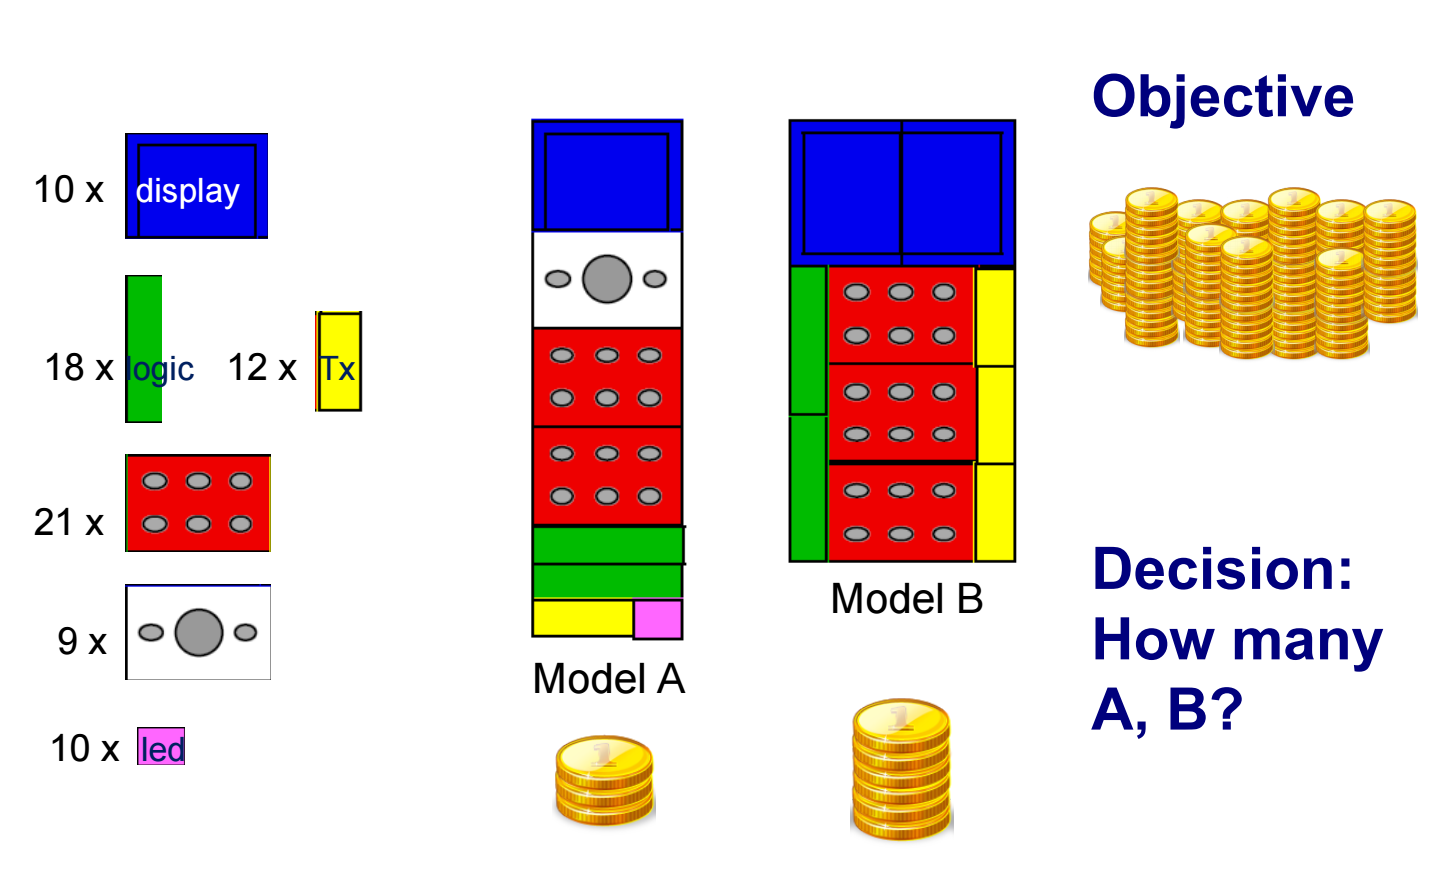
\includegraphics[width=0.7\textwidth]{images/l1-telefono.png}
\end{figure}

Per risolvere questo problema si possono usare varie strategie:

\begin{itemize}
	\item \textbf{Greedy}: scelgo di costruire il massimo numero di telefoni del modello con il prezzo più alto. Però non ho la garanzia che la soluzione trovata sia ottima.
	\item \textbf{Local search}: determino un certo numero di telefoni da produrre in modo da trovare una possibile soluzione sub-ottima per poi andare a modificare il numero di telefoni prodotti, cercando di migliorare il guadagno. Anche in questo caso non ho la garanzia che la soluzione trovata sia ottima.
	\item \textbf{Global search}: provo tutte le possibili combinazioni di telefoni che posso produrre, così facendo sono sicuro di trovare una soluzione ottima.
\end{itemize}


Un altro possibile problema è quello del contadino che possiede 12 ettari di terra dove può coltivare patate o pomodori, avendo a disposizione 70kg di semi di pomodoro, 18 tonnellate di tuberi di patate e 160 tonnellate di fertilizzante. Il contadino sa che un ettaro di campo coltivato a pomodori produce un guadagno di 3000 euro mentre uno di patate 5000. Per coltivare un ettaro a pomodori servono 7kg di semi e 10 tonnellate di fertilizzante, mentre un ettaro di patate richiede 3 tonnellate di tuberi e 20 di fertilizzante.

Questo problema è simile a quello del telefono, con la differenza che in questo caso gli ettari possono essere frazionati e quindi l'approccio combinatorio non può essere utilizzato.

L'idea è quindi quella di formulare un modello che descrive la soluzione ottima, anziché formulare un algoritmo che lo risolve.

Come prima cosa è necessario identificare le \textbf{variabili decisionali}, in questo caso $x_T$ e $x_P$ che rappresentano gli ettari coltivati. 
Poi si deve definire la \textbf{funzione obiettivo} che si vuole ottimizzare, in questo caso $\max 3000 x_T + 5000 x_P$.
Infine è necessario definire i \textbf{vincoli del problema} per modellare il consumo di risorse. In questo caso:

\begin{align*}
	x_T + x_P &\leq 12 \text{ vincolo sulla terra} \\
	7 x_T &\leq 70   \text{ vincolo sui semi di pomodoro} \\
	3 x_P &\leq 18 \text{ vincolo sui tuberi} \\
	10 x_T + 20 x_P &\leq 160 \text{ vincolo sul fertilizzante} 
\end{align*}

Con questa formulazione del problema non dico niente riguardo la soluzione del problema, ma posso utilizzare il modello creato per trovarla utilizzando dei metodi matematici dato che l'insieme di vincoli può essere visto come un sistema di disequazioni.

Un primo approccio è quello di partire da un valore di partenza della funzione obiettivo, ad esempio 27000 e provare a migliorarlo utilizzando la discesa di gradiente, fino a trovare un punto del piano che corrisponde ad un valore ottimo.
Con questo approccio posso anche dire che la soluzione trovata è ottima, perché tutte le altre soluzioni migliori richiedono un maggior numero di risorse.

\begin{figure}[htbp]
	\centering
	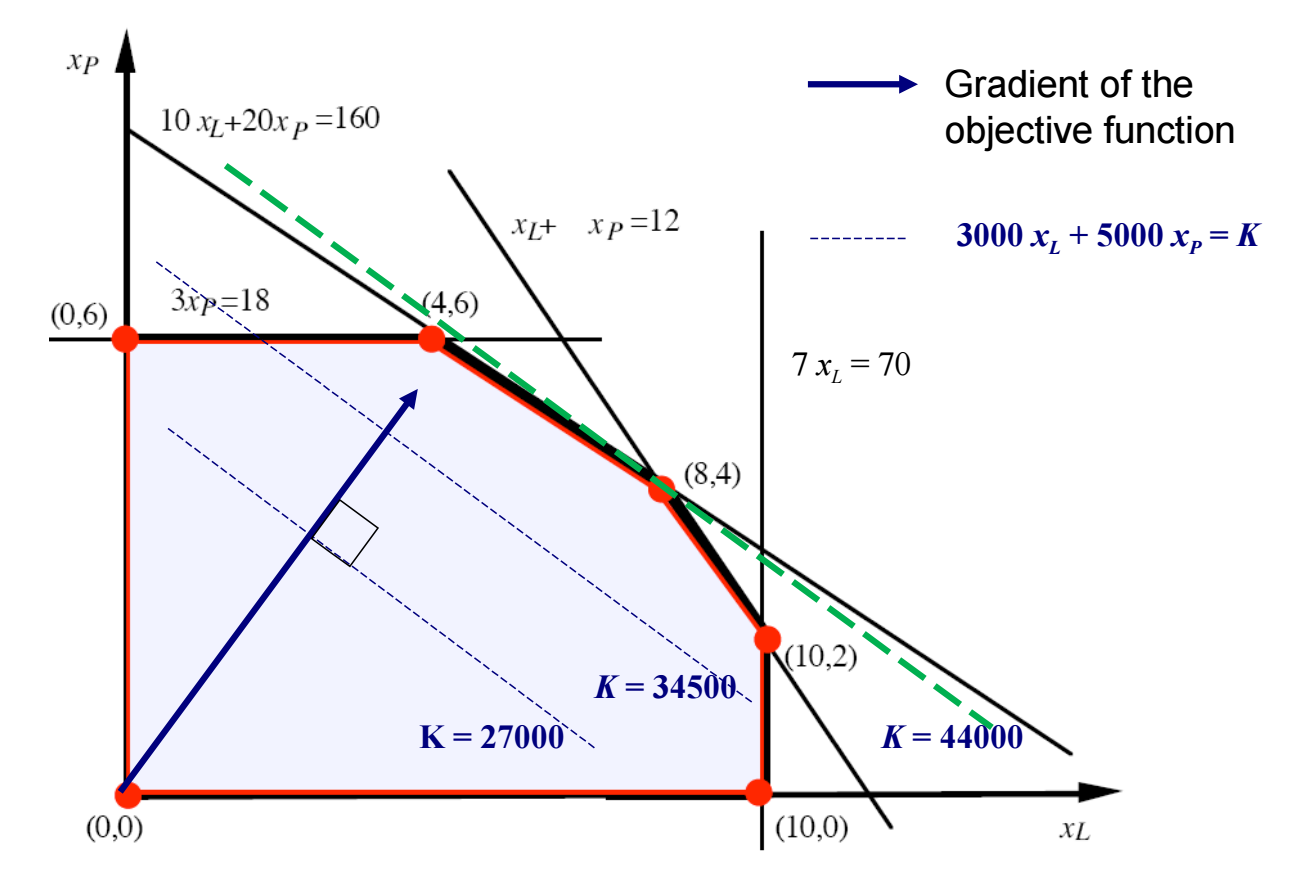
\includegraphics[width=0.5\textwidth]{images/l1-poligono.png}
\end{figure}


Tutto questo funziona perché sia i vincoli che la funzione obiettivo sono \textbf{lineari} e le variabili sono numeri reali. Questo tipo di modelli prende quindi il nome di \textbf{Linear Programming}.

Da notare che in questo caso la soluzione ottima è su un vertice intero, ma è un caso. Se le variabili utilizzate possono essere solo intere la situazione diventa più complessa perché è necessario effettuare delle approssimazioni.

\section{Approccio della ricerca operativa}

\begin{figure}[htbp]
	\centering
	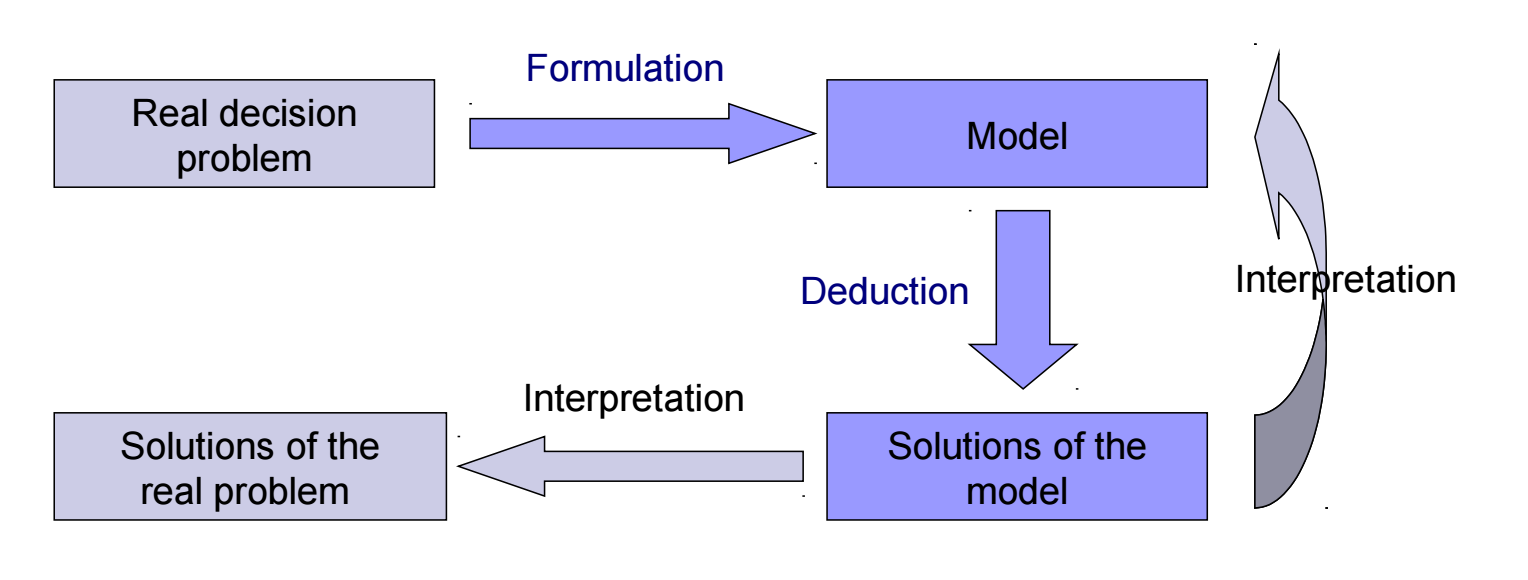
\includegraphics[width=0.7\textwidth]{images/l1-approccio.png}
\end{figure}

L'approccio precedentemente descritto è quello della ricerca operativa: si parte da un problema reale che viene formalizzato utilizzando un modello. Dal modello viene trovata una soluzione ottima per esso, la quale deve poi essere trasformata nella soluzione del problema reale.
Questo secondo passo può essere necessario perché nel modellare il problema può essere che sia stato necessario modificare alcuni vincoli, oppure utilizzare delle variabili reali anziché intere.

Si possono quindi definire due fasi: una di \textbf{formulazione} del modello e una di \textbf{deduzione} della soluzione, utilizzando alcuni algoritmi già definiti o personalizzati.

\section{Programma del corso}

\begin{enumerate}
	\item Ripasso e approfondimento delle tecniche di programmazione lineare e della dualità.
		\begin{itemize}
			\item Modelli LP, metodo del simplesso, teorema della dualità.
			\item Column generation technique per modelli LP grandi. Ovvero la creazione di modelli dinamici per evitare le limitazioni della memoria.
			\item Applicazioni: pianificazione della produzione, gestione del flusso di rete.
		\end{itemize}
	\item Metodi avanzati per la programmazione lineare intera mista (\textbf{MILP}).
		\begin{itemize}
			\item Formulazioni alternative, Branch \& Bound, Branch \& Cut.
			\item Applicazioni: Traveling Salesman Problem, localizzazione dei magazzini, set cover.
		\end{itemize}
	\item Meta euristiche per l'ottimizzazione combinatoria.
		\begin{itemize}
			\item Neighbourhood search e varianti.
			\item Algoritmi genetici.
		\end{itemize}
	\item Network optimization: modellazione dei problemi di ottimizzazione con i grafi. \textit{Potrebbe non essere affrontato.}
	\item \textbf{Laboratorio}:
		\begin{itemize}
			\item Online optimization server
			\item Optimization software and Algebraic modelling languages
			\item Optimization libraries (Cplex, Coin-OR, Scip)
		\end{itemize}
\end{enumerate}


\section{Informazioni pratiche}

Ci saranno dei laboratori nell'orario delle lezioni, verrà specificato nel sito quando ci saranno.

Non ci sono libri, vengono fornite le dispense dal professore e saranno in inglese.

Per ottenere il software che verrà utilizzato il laboratori è necessario registrarsi sul sito \url{http://www.math.unipd.it/userlist/subscribe/?idlist=277}, utilizzando la chiave \texttt{MeMoCO.16}. Per scaricare gratuitamente CPlex Optiumization Suite è necessario registrarsi alla IBM Academic Initiative.

L'esame è composto da:

\begin{itemize}
	\item Due esercitazioni di laboratorio, una sulla modellazione MILP e una sulle meta-euristiche, da consegnare qualche giorno prima dell'orale. Da fino a 10 punti.
	\item Esame orale che consiste nella discussione delle esercitazioni di laboratorio e delle domande teoriche sui contenuti del corso. Da fino a 20 punti. Forse si può fare in italiano.
	\item Progettino opzionale per ottenere un bonus da 2 a 6 punti. Il progetto riguarda la modellazione di un problema accordato con il docente e risolto utilizzando delle meta-euristiche o in modo esatto. Può essere fatto anche dopo lo scritto.
\end{itemize}



	% !TEX encoding = UTF-8
% !TEX program = pdflatex
% !TEX root = AALP.tex
% !TEX spellcheck = it-IT

% 6 Ottobre 2016

\chapter{Il mini linguaggio funzionale}

\section*{Testi di riferimento}

\begin{itemize}
	\item Types and Programming Languages (B. Pierce) 
	\item Practical Foundations for Programming Languages - Capitoli 1 e 2, consigliato leggerli prima della prossima lezione
\end{itemize}

\section{Teoria dei linguaggi di programmazione}

Si vuole descrivere il comportamento dei programmi in un modo preciso e formale, definendo una sintassi e una semantica.
Definire la sintassi è abbastanza semplice, la semantica è invece più complessa perché può avere varie sfumature:

\begin{itemize}
	\item \textbf{Semantica operazionale}: descrive come evolve la computazione del programma.
	\item \textbf{Semantica denotazionale}: descrive il programma in termini matematici, come una relazione tra l'input e l'output.
	\item \textbf{Semantica assiomatica}: descrive il programma utilizzando delle proprietà che sono vere per un certo programma, per poi utilizzarle per derivarne di nuove.
\end{itemize}

\noindent Noi ci concentreremo sulla semantica operazionale che viene verificata mediante tecniche di analisi statica sfruttando: sistemi di tipi, logiche temporali e interpretazione astratta.
Una volta fissato un sistema di tipi, questa verifica del programma può anche essere automatizzata.

\section{Linguaggi funzionali}

Studiare i tipi risulta più semplice sui linguaggi funzionali che su quelli imperativi.
Inoltre, lo stile di programmazione funzionale risulta più elegante perché è concentrato sul \textit{``what to do''} anziché \textit{``how to do''}.

\begin{lstlisting}[language=Java, caption=Confronto tra Java 5 e Java 8: nel secondo caso è subito chiaro l'intento del programmatore inoltre non vengono aggiunte variabili \textit{mutable}. Tuttavia l'esempio non usa le caratteristiche funzionali di Java8]
// Java 5
boolean found = false;
for(String city : cities){
	if (city.equals("Chicago")) {
		found=true;
		break;
	}
}
System.out.println("Found?" + found);
	
// Java 8
System.out.println("Found?" + cities.contains("Chicago"));
\end{lstlisting}

\begin{lstlisting}[language = Java, caption=Confronto tra Java 5 e Java 8: l'utlilizzo delle funzioni lambda rende il codice più conciso. Inoltre non vengono usate variabili mutabili e il codice è facilmente parallelizzabile.]
// Java 5
Collection<Person> people = ...;
int maxAge = -1;
for (Person p : people) {
	if (p.getGender() == MALE && p.getAge() > maxAge){
		maxAge = p.getAge();
	}
}

// Java 8
Collection<Person> people = ...;
final int maxAge = people.stream()
										      .filter(p -> p.getGender() == MALE)
										      .mapToInt(p -> p.getAge())
										      .max();
\end{lstlisting}

\noindent Tra le caratteristiche distintive dei linguaggi funzionali c'è l'\textbf{assenza degli assegnamenti}: ci sono delle variabili ma queste rappresentano dei valori e non delle aree di memoria modificabili. Vengono quindi solamente rappresentati dei valori immutabili.

Segue quindi che non ci sono side-effects: la chiamata di una funzione può essere sostituita con il suo risultato (\textbf{referential transparency}). Questo non è più valido se ad esempio la funzione stampa qualcosa a video e poi ritorna un risultato, pertanto se una funzione è pura, questa non può neanche produrre delle stampe a video.

Sembra una limitazione, ma in realtà così facendo si hanno vari vantaggi:
\begin{itemize}
	\item Il codice diventa più affidabile e più riusabile.
	\item Due funzioni che lavorano su dati diversi come \texttt{f(x)} e \texttt{g(y)} possono essere eseguite in parallelo senza problemi.
	\item Tutto ciò che entra ed esce dalla funzione può essere sottoposto a type check e quindi al compilatore basta solo il prototipo. Inoltre, se c'è un errore logico nella definizione della funzione è facile che questo si rifletta anche in un errore di tipo.
\end{itemize}

\noindent Un'altra caratteristica chiave è che le funzioni sono oggetti \textbf{first class}, ovvero sono a tutti gli effetti degli oggetti che possono essere passati come parametro ad altre funzioni. 
Le funzioni che prendono in input altre funzioni vengono chiamate funzioni \textbf{higher order}.
Ciò permette di scomporre un problema in sotto-problemi, utilizzare delle funzioni semplici per risolvere i sotto-problemi, per poi combinare le funzioni utilizzando delle funzioni higher-order.

\section{Sintassi del nostro linguaggi $\mathcal{L}$}

\begin{align*}
	x \in Var & &\\
	n \in Num & &\\
	Termini \: M, N &::= x &\text{ variabili} \\
								&|\: n \:|\: \text{true} \:|\: \text{false} &\text{ costanti intere e booleane} \\
								&|\: M + M \:|\: M - M &\text{ operazioni intere} \\
								&|\: \text{if} \: M \: \text{then} \: M \: \text{else} \: M &\text{ condizionale} \\
								&|\: \text{fn } x.M &\text{ dichiarazione di una funzione} \\
								&|\: M \: M &\text{ applicazione di una funzione}
\end{align*}

\noindent Un programma è quindi un termine chiuso \textit{M}, ovvero che non ha variabili libere e l'esecuzione del programma equivale a trovare il valore del termine \textit{M}.

Alcuni esempi di programmi:

\begin{align*}
3 + 2 &\\
\text{fn} \:  x.x &\:\text{// funzione identità} \\
\text{fn} \: x.3 &\: \text{// funzione costante 3} \\
\text{fn} \: x.x+1 &\: \text{// funzione successore} \\
\text{fn} \: x.x+1 \: 3 &\: \text{// funzione successore applicata al numero 3} \\
\text{fn} \: x.\text{fn} \: y . x+y &\: \text{// funzione somma con due argomenti (currificata)} \\
\text{fn} \: x. (\text{fn} \: y . x+y   + 2) &\: \text{// funzione che ritorna la funzione $2+x$} \\
\underbrace{\text{fn} \: x.\text{fn}\ y.(x\: y)}_{M} &\: \text{// funzione che applica un'altra funzione} \\
(M \: \text{fn} \: z.z) \: 5 &\: \text{// applicazione della funzione identità al numero 5} \\
\text{if} \: 2 \: \text{then} \: \text{fn}\: x.x+x \: \text{else} \: 0 &\: \text{// utilizzo del condizionale, è sinteticamente corretto ma non a livello di tipi}
\end{align*}

\noindent Il comportamento dei programmi dipende poi dalla semantica che viene attribuita alle istruzioni.

\subsection{Variabili libere}

C'è poi il concetto di variabile \textbf{libera} o \textbf{legata}.
La variabile $x$ nel termine $\text{fn } x.x$ è legata, perché viene dichiarata dal termine, infatti $\text{fn}$ è un \textit{binder}.

Nel termine $x+y$ le due variabili sono libere, perché non si riesce ad attribuirgli un valore. Per funzionare un programma non deve avere variabili libere.
Mentre nel termine $\text{fn }y. x\: y$ la variabile $x$ è libera mentre la $y$ è legata. Si ottiene così una \textbf{clojure}, ovvero una funzione che per essere calcolata deve ricevere dei valori per le variabili libere.

Ci sono poi le funzioni \textbf{alpha-equivalenti}, ovvero funzioni che calcolano la stessa cosa, ma che utilizzano variabili legate con nomi diversi. Es: $\text{fn }y.y+1$ e $\text{fn }x.x+1$.

Più formalmente si possono definire le variabili libere in modo induttivo.
Dato un termine $M$, le variabili libere di $M$ vengono indicate con $fv(M)$ e sono definite induttivamente come:

\begin{align*}
	fv(x) &= \{ x \} \\
	fv(n) =fv(\text{true}) = fv(\text{false}) &= \emptyset \\
	fv(M + N) = fv(M-N) &= fv(M) \cup fv(N) \\
	fv(\text{if } M_1 \text{ then } M_2 \text{ else }M_3) &= fv(M_1) \cup fv(M_2) \cup fv(M_3) \\
	fv(\text{fn }x.M) &= fv(M) \setminus \{x\} \\
	fv(M \: N) &= fv(M) \cup fv(N)
\end{align*}

\noindent Un termine senza variabili libere viene detto \textbf{chiuso} e i programmi sono definiti da dei termini chiusi.

\subsection{Sostituzione}

Definiamo ora l’operazione di sostituzione di una variabile con un termine, necessaria per la definizione della semantica del linguaggio. 
Indichiamo con $M \{x := N\}$ il termine $M$ in cui la variabile $x$ è stata sostituita con il termine $N$.
Nel seguito useremo una notazione compatta in cui \textit{c} varia nell’insieme delle costanti intere e booleane, mentre $op(M_i)_{i\in I}$ varia nell’insieme delle operazioni aritmetiche e booleane.

\begin{align*}
	x \{x := N\} &= N \\
	y \{x := N\} &= y \\
	c \{x := N\} &= c \\
	op(M_i)_{i \in I}\{x := N\}  &= op(M_i\{x := N\} )_{i \in I} \\
	(M_1 + M_2) \{ x:= N \} &= M_1\{x := N\} + M_2 \{x := N\} \\
	(\text{fn} \: x.M)\{x := N\} &= \text{fn }x.M \\
	(\text{fn} \: y.M)\{x := N\}  &= \text{fn }y.M\{x := N\} \text{ if } y \notin fv(N) \\
	(M_1 \: M_2) \{x := N\}  &= (M_1\{x := N\} \: M_2 \{x := N\} )
\end{align*}

\noindent Quando applico una sostituzione $M\{x := N\}$ devo stare atteno a sostituire solamente le occorrenze libere di $x$ ed è inoltre importante che i termini che vado ad aggiungere non vengano catturati da un altro binder.
Per evitare questo problema è necessario rinominare le variabili problematiche per alpha conversione.

Ad esempio $(\text{fn }x.x)\{x := 3\}$ \textbf{non} è $\text{fn }x.3 $ ma $\text{fn }x.x$ e allo stesso modo $(\text{fn }y.x+y)\{x := y\}$ \textbf{non} è $\text{fn }y.y+y$ ma $(\text{fn }x.x+z)\{x := y\} = \text{fn }z.y+z$.






	% !TEX encoding = UTF-8
% !TEX program = pdflatex
% !TEX root = InformationRetrieval.tex
% !TEX spellcheck = it-IT

% 6 Ottobre 2016

%\chapter{Rappresentazione dei documenti}
%\section{Analisi automatica del testo}

Tutto è iniziato quando George K. \textbf{Zipf}, uno studioso americano di linguistica ha formulato delle leggi empiriche che mettono in relazione la \textbf{frequenza di una parola} con la sua \textbf{forma} e \textbf{significato}. 
Solo in un secondo momento queste leggi sono state applicate all'indicizzazione dei documenti.

L'osservazione di partenza è stata quella che ci sono poche parole che sono veramente molto frequenti, come gli articoli, e che sono poco significative rispetto il contenuto informativo del documento. Ci sono poi tante parole poco frequenti, alcune delle quali sono fortemente correlate al contenuto informativo del documento. Il gioco è quindi quello di sfruttare al meglio tali parole.

Questo andamento può essere rappresentato graficamente, prima andando a contare le frequenze delle singole parole, per poi andare ad ordinarle da quella più frequente a quella meno frequente. La distribuzione così ottenuta è intera, ma può essere approssimata da un'iperbole.

Tipicamente in inglese:
\begin{itemize}
	\item Le due parole più frequenti sono \textit{the} e \textit{of}, mediamente sono il 10\% delle parole del documento.
	\item Le 6 parole più frequenti corrispondo a circa il 20\% delle occorrenze e le 50 parole più frequenti corrispondo a circa il 40\% dei testi. Questo deriva dal fatto che la lingua deve essere ridondante in modo che sia facile da capire.
	\item Considerando un'insieme di documenti molto ampio, circa la metà delle singole parole di quel campione compare una sola volta. Queste sono parole più significative dal punto di vista dell'informazione. Tuttavia è necessario tenere conto che in questo insieme di parole possono comparire anche gli errori di battitura.
\end{itemize}

\subsection{Legge di Zipf}

La legge di Zipf afferma che dato un campione di testi e calcolata la frequenza $f$ delle parole, una volta che si sono messe le parole in ordine decrescente di frequenza, cioè si sono ordinate le parole in base al ragno \textit{r}, la distribuzione che si ottiene ha un andamento assimilabile ad una iperbole e si ha che

$$
r \times f = k
$$

ovvero la distribuzione è data da $ f = \cfrac{k}{r}$.

Se anziché ragionare in termini di frequenza assoluta si passa a considerare quella relativa, ovvero la probabilità osservata di occorrenza della parola, la legge di Zipf può essere riscritta come 

$$
r \times P_r = c
$$

Dove $P_r$ è la probabilità di occorrenza della parola che occupa il rango $r$-esimo e $c$ è una costante ($c = 0.1$ per l'inglese).

Si ha che per la lingua inglese $c \approx 0,1$ e l'iperbole che si ottiene è riportata in figura \ref{fig:zipf}

\begin{figure}[htbp]
\centering
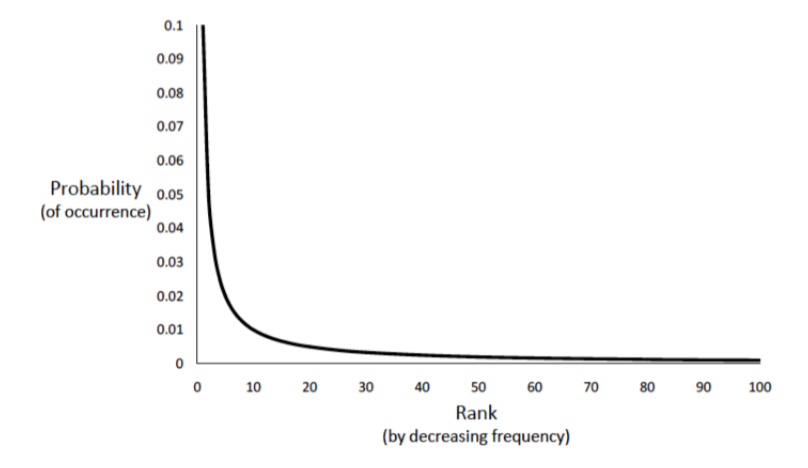
\includegraphics[width=0.55\linewidth]{images/l3-zipf}
\caption{Rango rispetto la probabilità di occorrenza assumendo valida la legge di Zipf con $c = 0.1$}\label{fig:zipf}
\end{figure}

\subsection{Indicazioni di H.P. Luhn}

L'idea per l'indicizzazione è quindi quella di definire due soglie di \textit{cut-off} per evitare di prendere in considerazione le parole troppo frequenti, perché poco significative, e quelle troppo poco, per limitare l'effetto degli errori di battitura.

Ogni parola ha un certo \textbf{resolving power}, ovvero una certa capacità di discriminare il contenuto del documento da quello degli altri e di caratterizzare il contenuto della collezione.

\begin{figure}[htbp]
	\centering
	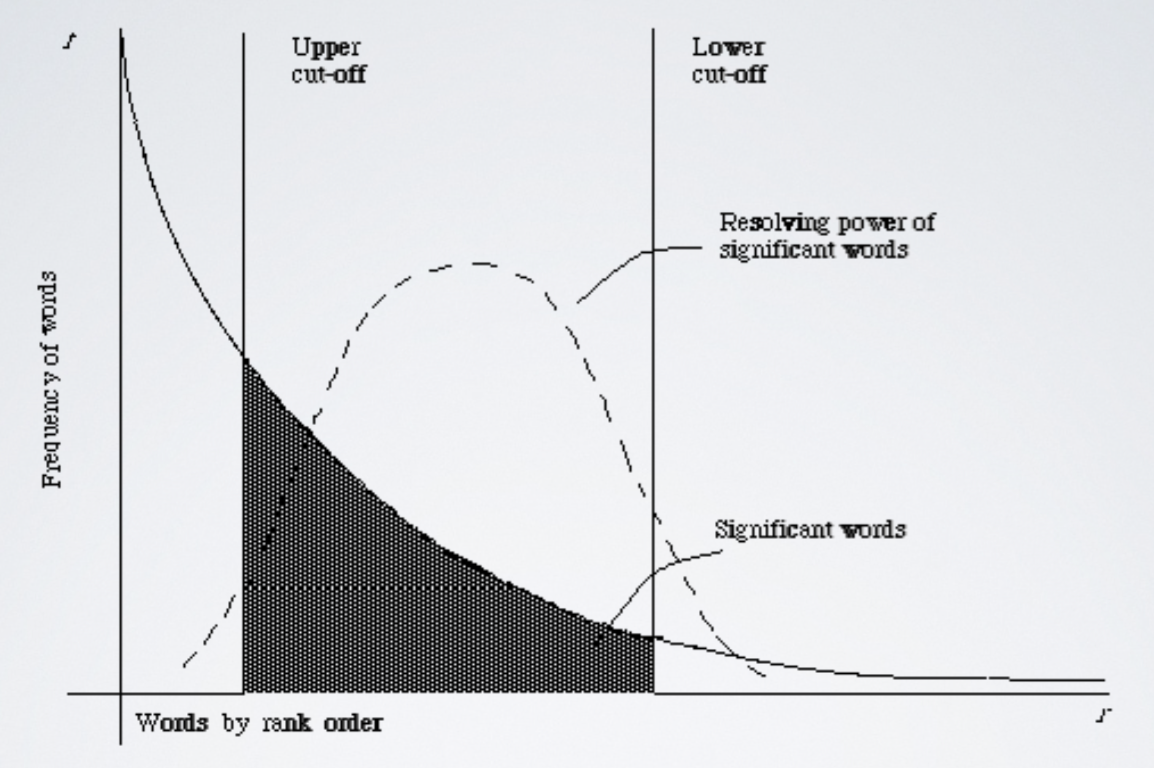
\includegraphics[width=0.55\linewidth]{images/l3-cutoff}
	\caption{Plot della curva $r \times f$ che evidenzia la posizione delle parole significative.}
\end{figure}

Questo vale per le collezioni generiche dei documenti, mentre se si parla di un argomento specifico si può dare maggiore peso a determinate parole. Ad esempio può capitare che se viene preso in esame un manuale di MySQL è ovvio che le parole ``MySQL'' e  ``table'' compariranno tante volte anche se non sono articoli.

C'è anche un altro discorso relativo alla forma plurale delle parole, che in conteggio di frequenza viene considerata come una parola diversa, quando in realtà può essere che abbia lo stesso valore informativo della forma singolare. In alcuni casi è quindi opportuno sommare le occorrenze della forma plurale e di quella singolare.

Si ha quindi che i passi per applicare le indicazioni di Luhn sono:

\begin{itemize}
	\item Si calcoli la frequenza di ogni descrittore in ogni documento della collezione di riferimento. C'è inoltre da scegliere come trattare le parti di contorno dei documenti come l'indice, la premessa, ecc. tali parti tipicamente non vengono considerate.
	\item Si calcoli la frequenza totale di ogni descrittore.
	\item Si ordino i descrittori per frequenza decrescente.
	\item Si scelga una soglia di \textit{upper cut-off} e si rimuovano dalla lista i descrittori con frequenza superiore alla soglia. In questo modo si rimuovono gli articoli, le preposizioni, ecc.
	\item Si scelga un'altra soglia di \textit{lower cut-off} e si rimuovano dalla lista i descrittori con frequenza inferiore al valore di soglia. In questo modo si rimuovono i descrittori ``rumore''  o che non apportano alcun contribuito alla descrizione del contenuto.
\end{itemize}

\noindent Entrambe le soglie possono essere calcolate in modo euristico.

Le parole che vengo eliminate dalle soglie di cut-off vengono nominate \textbf{stop word} e sono raccolte nella lista che prende il nome di \textbf{stop list}.


\textbf{{\color{Red} Possibile esercizio:}} Domande relative alle osservazioni proposte da Zipf e Luhn.

\section{Indicizzazione}

L'indicizzazione ha l'obiettivo di rappresentare il contenuto informativo di un documento e nel tempo questo processo ha preso una struttura a fasi.
Il documento viene rappresentato da dei descrittori che vengono utilizzati per la costruzione degli indici utili al reperimento dell'informazione.

Quindi l'indicizzazione fornisce automaticamente una rappresentazione più compatta e direttamente utilizzabile del contenuto informativo del documento. Gli indici sono utilizzati come surrogati del contenuto del documento durante la fase di reperimento.

L'indicizzazione può essere svolta:
\begin{itemize}
	\item manualmente
	\item in modo automatico
	\item in modo semi-automatico, quando è necessario intervenire all'interno del processo per prendere delle decisioni che non possono essere prese in modo automatico.
\end{itemize}

\noindent Tutti questi metodi funzionano estraendo direttamente dal documento le informazioni. Tuttavia possono essere estesi in modo che vengano presi in considerazione anche dei dizionari o delle meta-informazioni.

\begin{figure}[htbp]
	\centering
	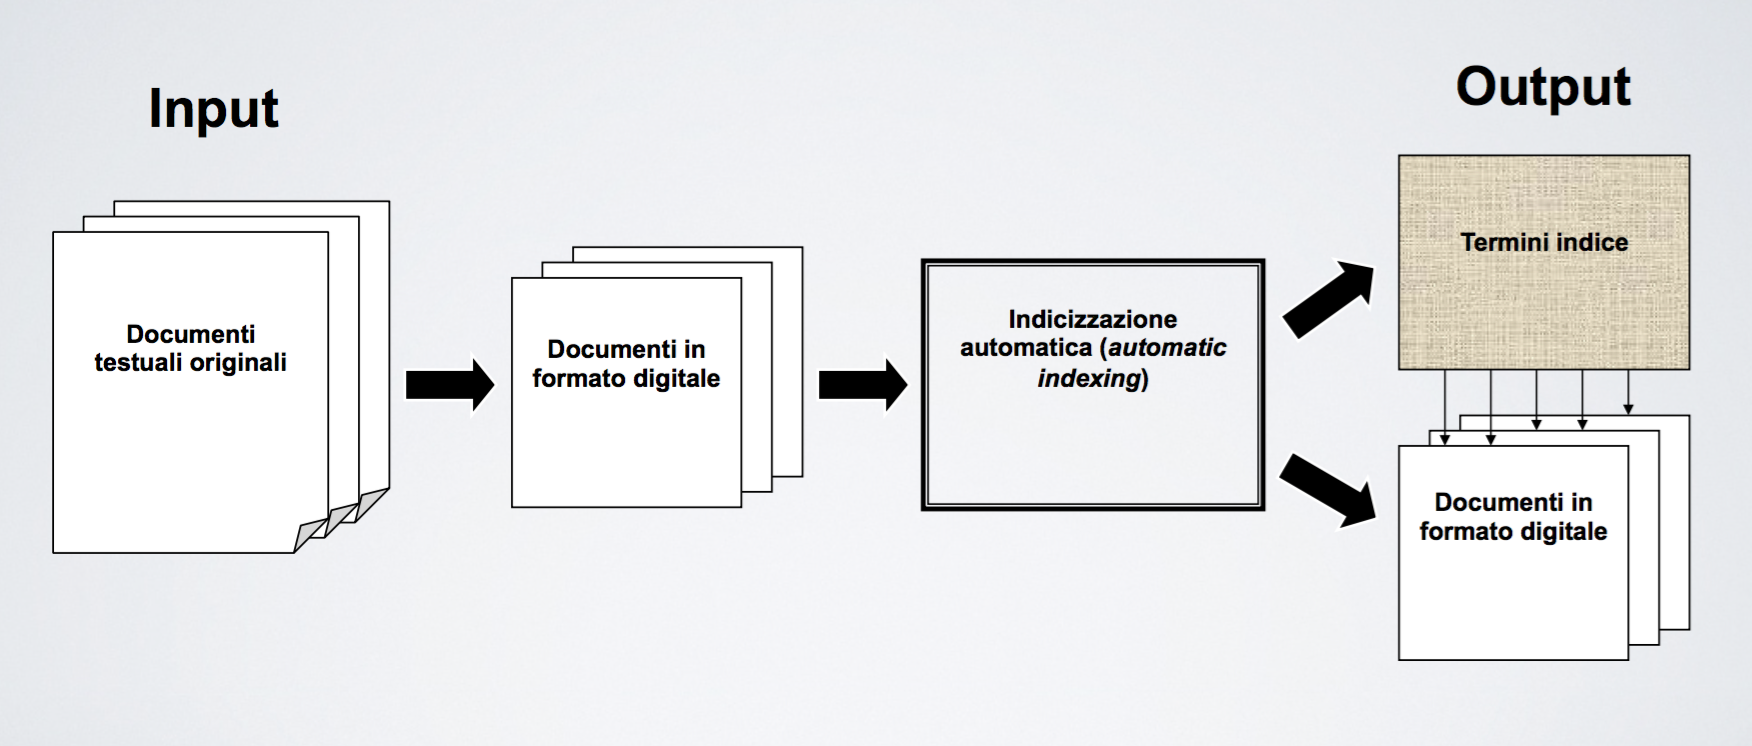
\includegraphics[width=0.7\linewidth]{images/l3-indicizzazione}
	\caption{Schema generale dell'indicizzazione}
\end{figure}

\subsection{Indicizzazione automatica dei testi}

L'indicizzazione automatica di un documento testuale è un processo che esamina automaticamente gli oggetti informativi (parole, frasi, didascalie, figure, ecc.) che compongono il documento e produce una lista di termini indice presenti nell'intera collezione dei documenti.

L'estrazione dei termini indice viene fatta da appositi algoritmi e, una volta estratti, questi vengono collegati ai diversi documenti che li contengono.
Così facendo durante il reperimento sarà sufficiente fare riferimento ai termini indice e non all'intera collezione.

\subsection{Attuazione dell'indicizzazione automatica}

L'indicizzazione automatica dei documenti testuali viene eseguita in più fasi, che devono essere attuate in sequenza:

\begin{enumerate}
	\item Analisi lessicale e selezione delle parole.
	\item Eventuale rimozione delle stop word.
	\item Riduzione delle parole originali alle rispettive radici (\textit{STEM}). Ad esempio le forme plurali vengono ridotte a quelle singolari.
	\item Composizione dei termini. Come ad esempio ``information retrieval''. Ovvero le parole vengono combinate tra loro quando si trovano ad una determinata distanza.
	\item Creazione dell'indice.
	\item Eventuale pesatura degli elementi dell'indice. 
\end{enumerate}

Alla fine di queste fasi l'indice sarà composto da parole, termini e frasi che noi riteniamo significative, assieme alle informazioni del peso che gli diamo e alla loro frequenza all'interno dei documenti.









	\chapter{Laboratorio}

\section{Un po' di cose su R}\label{un-po-di-cose-su-r}

\begin{itemize}
\item
  Tutti gli oggetti sono vettori
\item
  \texttt{ls()} per vedere le variabili disponibili
\item
  \texttt{x\ \textless{}-\ c(2,3,4,5)} crea un vettore con 1,2,3,4.
\item
  notazione \texttt{{[}1:20{]}} per un vettore con la successione da 1 a
  20
\item
  \texttt{xx\ \textless{}-\ seq(from=100,\ to=1)} crea sempre una
  sequenza di numeri, con parametro opzionale \texttt{by} per
  specificare lo step
\item
  \texttt{rep(2,5)} crea un vettore con 5 elementi uguali a 2
\item
  \texttt{a\ \textless{}-\ c(rep(2,3),4,5,rep(1,5))},
  \texttt{a\ =\ 2\ 2\ 2\ 4\ 5\ 1\ 1\ 1\ 1\ 1}
\item
  \texttt{2*x} esegue il prodotto scalare
\item
  \texttt{length(x)} per la lunghezza del vettore
\item
  \texttt{max(x)} e \texttt{min(x)}
\item
  \texttt{sum(x)} che ritorna un vettore di un solo elemento con la
  somma
\item
  \texttt{mean(x)}, \texttt{var(x)}, \texttt{range(x)}
\item
  \texttt{x{[}7{]}} per estrarre il settimo elemento di \texttt{x},
  l'indice credo parta da 1
\item
  \texttt{x{[}-4{]}} ritorna un vettore senza il quarto elemento
\item
  \texttt{x\ \textless{}-\ matrix(c(2,3,5,7,11,13),nrow\ =\ 3)} crea una
  matrice con gli elementi specificati e 3 righe. Alternativamente è
  possibile specificare anche il numero di colonne.
\item
  \texttt{x2\ \textless{}-\ scan("nome\ file",\ sep="")} con
  \texttt{sep} opzionale, per caricare il contenuto di un file in un
  vettore, per caricare una matrice
  \texttt{x2\ \textless{}-\ matrix(scan(...),\ ncol\ =\ 3,\ byrow=TRUE}.
\item
  \texttt{str(x)} specifica la struttura dell'oggetto
\item
  \texttt{dim(x)} ritorna la dimensione di una matrice, se invocato con
  un vettore ritorna \texttt{NULL}.
\item
  \texttt{x{[}18,{]}} per ottenere la 18-esima riga di una matrice
\item
  \textbf{Dataframe}: matrice le cui colonne possono avere formati
  diversi
\item
  \texttt{ciliegi\ \textless{}-\ read.table("nome\ file")}.
\item
  \texttt{names(ciliegi)} è il vettore con i nomi delle colonne del
  dataframe
\item
  \texttt{names(ciliegi)\ \textless{}-\ c("diametro",\ "altezza",\ "volume")}
  permette di impostare il nome delle colonne, può anche essere
  specificato come parametro opzionale \texttt{col.names} della
  funzione \texttt{read.table}.
\item
  \texttt{summary(ciliegi)} fornisce degli indicatori per ciascuna
  colonna
\item
  \textbf{Mediana}: elemento centrale di una distribuzione ordinata in
  senso crescente, \textbf{primo e terzo quartile}: generalizzazione
  della mediana, rispettivamente l'elemento che sta al 25 e 75 per cento
  della distribuzione. La differenza tra i due quartili da l'idea di
  quanto è variabile la distribuzione.
\item
  I dataframe possono essere acceduti anche con il nome della colonna
  \texttt{ciliegi\$volume}.
\item
  \textbf{attach di un file}: aggiungere al workspace un oggetto, ovvero
  \texttt{attach(ciliegi)} permette di accedere al nome della colonna
  direttamente utilizzando \texttt{volume}. Come complementare c'è il
  comando \texttt{detach}.
\item
  \texttt{hist(diametro)} crea l'istogramma per il diametro
\item
  \texttt{help(hist)} per avere l'help di una funzione
\item
  l'istrogramma che viene generato di default può contenere dei buchi,
  conviene quindi adattare il numero di colonne utilizzando il parametro
  \texttt{breaks}
\item
  \texttt{boxplot(diametro)} fornisce il box plot di un valore, è un
  grafico che rappresenta la mediana, i quartili e il 5 e 95\%. Risulta
  più espressivo dell'istogramma. L'ampiezza della scatola rappresenta
  la variabilità dei dati.
\item
  \texttt{ciliegi{[}altezza\textgreater{}80,{]}} prende tutti i ciliegi
  con altezza maggiore di 80.
\item
  \texttt{library(MASS)} permette di caricare la libreria MASS
\item
  \texttt{search()} permette di visualizzare la lista degli ottetti in
  cui R va a cercare quando deve eseguire un comando
\item
  Gli attributi qualitativi vengono trattati come tipo Factor
\item
  \texttt{table(painters\$School)} crea la tabella con le frequenze
  delle varie qualità
\item
  \texttt{barplot(..)} fa il plot delle barre per una variabile discreta
\item
  \texttt{pie(...)} fa il grafico a torta, anche se è sconsigliabile
  utilizzare un grafico a torta perché per l'occhio umano fa fatica a
  vedere la differenza tra gli angoli.
\item
  come scale colori si possono utilizzare \texttt{heat.colors(k)},
  \texttt{rainbow(k)}, \ldots{}
\item
  \texttt{plot(x,y)} disegna un diagramma di dispersione, il parametro
  \texttt{pch} specifica il tipo di carattere, \texttt{pch=16}
  rappresenta i pallini pieni, \texttt{col} specifica il colore da
  utilizzare, possono indicare \texttt{col=painter\$School} per far
  variare il colore in base al valore dell'attributo quantitativo
\end{itemize}

	% !TEX encoding = UTF-8
% !TEX TS-program = pdflatex
% !TEX root = ../apprendimento_automatico.tex
% !TEX spellcheck = it-IT
\section{Lezione 5 - VC-Dimension e VC-Confidence}\label{lezione-5-vc-dimension-e-vc-confidence}

\subsection{Esempi di spazi delle ipotesi}\label{esempi-di-spazi-delle-ipotesi}

Seguono alcuni esempi di spazi per le ipotesi nei problemi di
apprendimento supervisionato, cioè quei problemi in cui si vuole
stabilire se un elemento \emph{x} appartiene o meno ad una classe.

\subsubsection{Iperpiani in R2}\label{iperpiani-in-r2}

\textbf{Iperpiano}: dato uno spazio a \emph{n}-dimensioni, un iperpiano
per quello spazio è un sottospazio di dimensione \emph{n-1}. Ad esempio gli
iperpiani in $R^2$ sono tutte le rette del piano.

Lavorando in $R^2$ lo spazio delle istanze è definito come:

$$
X = \{x | x \in R^2\}.
$$

Mentre lo spazio delle ipotesi è dato dalle dicotomie indotte da iperpiani in $R^2$, cioè da tutte le possibili divisioni del piano.

$$
H = \{f_{(w,b)}(x) | f_{(w,b)}(x) = sign(w \times x + b), w \in R^2, b \in R\}
$$

Così facendo vengono prese in considerazione tutte le rette che dividono
$R^2$ in due parti in modo che da una parte l'ipotesi valga 1 e dall'altra
-1.

\subsubsection{Dischi in $R^2$}\label{dischi-in-r2}

Sempre in $R^2$ è possibile considerare come spazio delle ipotesi tutte le
dicotomie indotte da dischi in $R^2$ e centrati nell'origine.

$$
H = \{f_b(x) | f_b(x) = sign(||x||^2 - b), w \in R^2, b \in R\}
$$

Il che vuol dire che all'interno del disco le ipotesi valgono -1 mentre
al di fuori valgono 1.

\subsubsection{\texorpdfstring{Congiunzione di \emph{m} letterali positivi}{Congiunzione di m letterali positivi}}\label{congiunzione-di-m-letterali-positivi}

Lo spazio delle istanze questa volta è dato da tutte le stringhe di \emph{m} bits

$$
X = \{s | s \in \{0,1\}^m\}
$$

Lo spazio delle ipotesi è dato da tutte le sentenze logiche che
riguardano i letterali positivi $l_1$,$l_2$,\ldots{},$l_m$ ($l_i$ è vero se
l'\emph{i}-esimo bit è 1) e che contengono solo l'operatore $\wedge$.

$$
H = \{ f_{(i_1,\ldots,i_j}(s) | f_{(i_1,\ldots,i_j}(s) \text{ equivale a } l_{i_1} \wedge l_{i_2} \wedge \ldots \wedge l_{i_j}, \{i_1\ldots{}i_j\} \text{ sottoinsieme di }  \{1..m\}\}
$$

\subsection{Misurare la complessità dello spazio delle ipotesi}\label{misurare-la-complessituxe0-dello-spazio-delle-ipotesi}

Considerato un determinato spazio delle ipotesi \emph{H}, questo
contiene sempre:

\begin{itemize}
\item
  L'\textbf{ipotesi più specifica}: ipotesi più stretta e consistente con
  i dati, nell'esempio del disco è il disco più stretto in grado di
  contenere tutti i punti negativi.
\item
  L'\textbf{ipotesi più generale}: quella più grande e consistente con i
  dati, sempre nell'esempio del disco, è quello più grande
  possibile che non contiene punti positivi.
\end{itemize}

\textbf{Shattering}: (frammentazione), dato \emph{S} sottoinsieme dello
spazio delle istanze, si dice che \emph{S} è frammentato dallo spazio
delle ipotesi \emph{H} se:

$$ 
\forall S' \in S, \exists h \in H, \text{ tale che } \forall x \in S, h(x) = 1 \text{ se e solo se } x \in S'.
$$

Cioè \emph{H} realizza tutte le possibili dicotomie di \emph{S}.

\emph{H} frammenta un certo insieme \emph{S} se è possibile trovare un
iperpiano \emph{h} che raccoglie tutti i punti dell'insieme \emph{S}. Ovvero per
tutte le dicotomie di \emph{S} esiste un iperpiano che riesce a
realizzarle.

\subsubsection{VC (Vapnik-Chervonenkis) Dimension}\label{vc-vapnik-chervonenkis-dimension}

La VC-Dimension è la dimensione di uno spazio delle ipotesi \emph{H}
definito su uno spazio delle istanze \emph{X} ed è data dalla
cardinalità del sottoinsieme più grande frammentato da \emph{H}.

$$
VC(H) =
\begin{cases}
max_{S \subseteq X} |S|&\text{ tale che \emph{H} frammenta } S  \\
 \infty& \text{ se S non è limitato}
\end{cases}
$$


Ad esempio se nello spazio delle ipotesi dato dagli iperpiani su $R^2$ ho 2 punti, lo spazio delle istanze viene frammentato da
\emph{H}, perché posso sempre trovare una retta che riesce a realizzare
tutte le possibili dicotomie di due punti su un piano.
Se nello spazio delle istanze ho 3 punti, riesco comunque a realizzare
tutte le dicotomie.
Se nello spazio delle istanze ho 4 punti qualsiasi non si riesce a
trovare un iperpiano che realizza la dicotomia, quindi \emph{VC(H) =
3}.

Segue che, prendendo uno spazio delle ipotesi di cardinalità finita si
ha che:

$$
VC(H) \leq log_2(|H|)
$$

Questo perché per ogni \emph{S} frammentato da \emph{H}, abbiamo
$|H| \geq 2^{|S|}$,
cioè per ogni dicotomia in \emph{S} esiste un ipotesi in \emph{H} che la
realizza, ovvero devono essere disponibili in \emph{H} tante ipotesi
quanti sono le dicotomie in \emph{H}.

Scegliendo un \emph{S} tale che $|S| = VC(H)$, si
ottiene $|H| \geq 2^{|S|}$, prendendo
il logaritmo si trova quello che si stava cercando, ovvero $VC(H) \leq log_2(|H|)$.

\textbf{Dal libro}:

Se un dataset contiene \emph{N} elementi, questi \emph{N} elementi
possono essere etichettati con degli 0 e 1 in $2^N$ modi diversi.

Se per ognuno di questi modi è possibile trovare un ipotesi $h \in H$
che separa tutte le istanze negative da quelle positive allora si dice
che \emph{H} frammenta il dataset \emph{N}. 
Il che vuol dire che il dataset \emph{N} può essere appreso con un errore empirico nullo.

Il massimo numero di punti che possono essere frammentati da \emph{H} è
detto \emph{VC(H)} e fornisce una misura della capacità di \emph{H}.

\subsection{Bound sull'errore di generalizzazione}\label{sec:vcc}

Considerando un problema di apprendimento binario, con:

\begin{align*}
\text{Training set }S &= \{(x_i,y_i), \ldots (x_N, y_N)\} \\
\text{Spazio delle ipotesi } H &=\{h_\theta(x)\} 
\end{align*}

Supponendo di avere un algoritmo di apprendimento \emph{L} che
restituisce l'ipotesi $h_{\theta*}$ che minimizza l'errore empirico su
\emph{S} espresso come $errore_S(h_\theta(x))$.

È possibile derivare un bound (limite superiore) per l'errore ideale o
errore di generalizzazione, valido con probabilità \emph{(1 - $\sigma$)} con
$\sigma$ piccolo a piacere:

$$
errore_D(h_\theta(x)) \leq  errore_S(h_{\theta}(x)) + g(N, VC(H), \sigma)
$$

Il primo termine $errore_S(h_{\theta}(x))$ dipende dall'ipotesi restituita
dall'algoritmo di apprendimento \textit{L}.

Il secondo termine $g(N, VC(H), \sigma)$ non dipende da \emph{L}, ma dal
numero di esempi di training utilizzati (inversamente proporzionale),
dalla \emph{VC-dimension} (direttamente proporzionale) e dalla
confidenza, ovvero dal termine $\sigma$.

Questo termine viene anche chiamato \textbf{VC-confidence} e risulta essere monotono rispetto al rapporto
$\frac{VC(H)}{N}$.

\textbf{Morale della favola}: la VC-Dimension sovrastima con confidenza $\sigma$ l'errore ideale.

\subsection{Structural Risk Minimization (SRM)}\label{sec:srm}

Approccio per la scelta dello spazio delle ipotesi proposto da Vapnik
che cerca di trovare un compromesso tra l'errore empirico e la
VC-Confidence.

Si considerano spazi delle ipotesi sempre più piccoli $H_1 \subseteq H2 \subseteq \ldots \subseteq H_n$ tali che $ VC(H_1) \leq VC(H_2) \leq \ldots \leq VC(H_n)$

Si seleziona lo spazio delle ipotesi $H_i$ che ha il valore del bound
sull'errore di generalizzazione più piccolo. ovvero la VC-Dimension minore.

\begin{figure}[htbp]
\centering
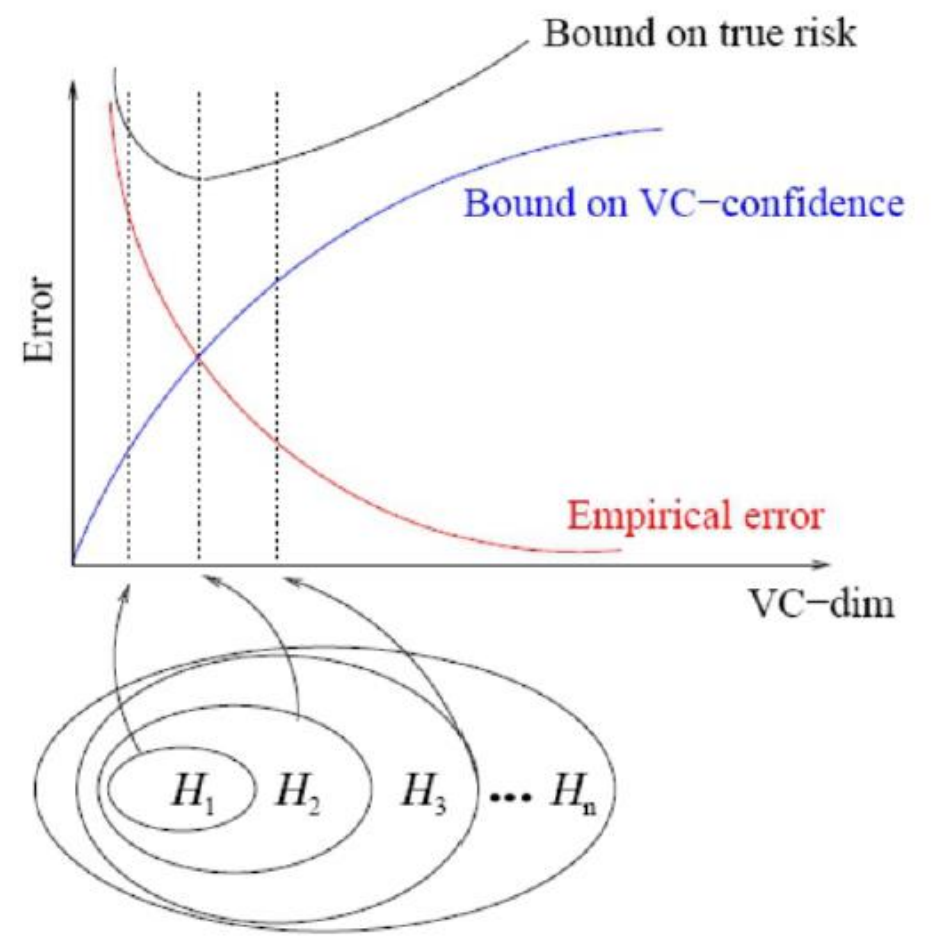
\includegraphics[width=0.5\textwidth]{./notes/immagini/l5-srm.png}
\caption{Structural Risk Minimization}
\end{figure}

	% !TEX encoding = UTF-8
% !TEX program = pdflatex
% !TEX root = AALP.tex
% !TEX spellcheck = it-IT

% 20 Ottobre 2016
% \section sistemi di tipi
% \subsubsection Teorema di Preservazione (Subject reduction)

% Dimostrazione del lemma di sostituzione (spostata al posto corretto in lezione5)

\subsubsection{Corollario di Subject-reduction}

\begin{center}
	Se $\emptyset \vdash M : T$ e $M \rightarrow^* M'$, allora $\emptyset \vdash M' : T$
\end{center}

\paragraph{Dimostrazione}

La dimostrazione viene fatta per induzione sul numero di passi che da $M$ portano ad $M'$.

Il caso base è quello con il cammino di lunghezza 0, ovvero quando $M = M'$ e la tesi è trivialmente vera.

Nel caso induttivo ho che $M \rightarrow^{*}_k M_1 \rightarrow M'$, pertanto per ipotesi induttiva ho che $\emptyset \vdash M_1 : T$. 

Ho poi che $M_1 \rightarrow M'$ e quindi posso applicare subject-reduction per ottenere che $\emptyset \vdash M' : T$.

\subsubsection{Teorema di Safety - Completo}

\begin{center}
	Se $\emptyset \vdash M : T $ e $M \rightarrow^* M'$ e $M' \not\rightarrow$, allora $M'$ è un valore.
\end{center}

\paragraph{Dimostrazione}

Alle due ipotesi posso applicare il corollario di subject-reduction, ottenendo che $\emptyset \vdash M' : T$.

Per il teorema di progressione ho poi che $M'$ è un valore oppure $M'$ fa un passo e va in $M''$, ma per ipotesi $M'$ non fa un passo e quindi $M'$ è per forza un valore.

\subsection{Esercizio sul typing}

Da notare che nel contesto iniziale non servono giudizi di tipo perché tutte le variabili che compaiono sono all'interno delle funzioni e che, non essendoci informazioni sui tipi, questi sono ignoti e pertanto è necessario fare anche inferenza durante la risoluzione dell'albero.

\begin{prooftree}	
	
	% App-1
	\AxiomC{$\checkmark$ $\textbf{\textit{T}} = \textbf{\textit{T}}_1 \rightarrow \textit{\textbf{T}}_3$}
	\LeftLabel{(\textsc{Var})}
	\UnaryInfC{$y : T, x : T' \vdash y : T_1 \rightarrow T_3$}
	
	% App-2
	\AxiomC{*}
	\LeftLabel{\textsc{(If)}}
	\UnaryInfC{$y : \textbf{\textit{T}}_1\rightarrow \textbf{\textit{T}}_3, x:T' \vdash \text{if true then }x \text{ else }y \: x : T_1$}
	\LeftLabel{\textsc{(App)}}
	\BinaryInfC{$y : T, x: T' \vdash y \: (\text{if true then }x \text{ else }y \: x) : \: T_3$}
	
	\LeftLabel{\textsc{(Fun)}}
	\UnaryInfC{$y : T \vdash \fn x : \textbf{\textit{T'}} . (y \: (\text{if true then }x \text{ else }y \: x)) : \textbf{\textit{T}}_2 = \textbf{\textit{T'}} \rightarrow \textbf{\textit{T}}_3$}
	
	\LeftLabel{\textsc{(Fun)}}
	\UnaryInfC{$\emptyset \vdash \fn y : \textbf{\textit{T}} . \fn x : T' . (y \: (\text{if true then }x \text{ else }x \: y)) : \textbf{\textit{T}} \rightarrow \textbf{\textit{T}}_2$} % T' \rightarrow ?
\end{prooftree}

\noindent Dal ramo sinistro di \textsc{(App)} riesco a chiudere con $T = T_1 \rightarrow T_3$ e quindi riporto l'informazione anche sul ramo destro.
La derivazione continua applicando \textsc{(IfThenElse)} e con $\Gamma = y:T_1 \rightarrow T_3, x:T'$:

\begin{prooftree}
	%if 1
	\AxiomC{$\checkmark$}
	\LeftLabel{\textsc{(True)}}
	\UnaryInfC{$\Gamma \vdash \true : \Bool$}
	
	%if 2
	\AxiomC{$\checkmark$  $\textbf{\textit{T}}_1 = \textbf{\textit{T'}}$}
	\LeftLabel{\textsc{(Var)}}
	\UnaryInfC{$y: T_1 \rightarrow T_3, x:T' \vdash x : T_1$}
	
	%if 3
	\AxiomC{**}
	\LeftLabel{\textsc{(App)}}
	\UnaryInfC{$y : \textbf{\textit{T'}} \rightarrow T_3, x:T' \vdash y \: x : \textbf{\textit{T'}}$}
	% per quello che ho scoperto 
	\UnaryInfC{$y : T_1 \rightarrow T_3, x:T' \vdash y \: x : T_1$}
	\LeftLabel{\textsc{(If)}}
	\TrinaryInfC{(*)$\Gamma \vdash \text{if true then }x \text{ else }y \: x : T_1$}
\end{prooftree}

\noindent Dal ramo centrale della regola \textsc{(IfThenElse)} scopro che $T_1 = T'$ e quindi aggiorno il ramo destro e il contesto, che ora è  $\Gamma = y:T' \rightarrow T_3, x:T'$.

\begin{prooftree}
	\AxiomC{$\checkmark$}
	\LeftLabel{\textsc{(Var)}}
	\UnaryInfC{$y:T' \rightarrow T_3 , x:T' \vdash y : T_4 \rightarrow T'$}
	
	\AxiomC{$\checkmark$}
	\LeftLabel{\textsc{(Var)}}
	\UnaryInfC{$y : T' \rightarrow T_3 , x :T'\vdash x : T_4$}
	
	\LeftLabel{\textsc{(App)}}
	\BinaryInfC{(**)$\Gamma \vdash y \: x : T'$}
\end{prooftree}

\noindent Da quest'ultimo albero trovo che $T' = T_4 = T_3$. Andando a sostituire il tutto trovo che:

\begin{itemize}
	\item $y : T' \rightarrow T'$
	\item $x : T'$
	\item $T_2 = T' \rightarrow T_3 = T' \rightarrow T'$
	\item $T = T_1 \rightarrow T_3 = T' \rightarrow T'$
	\item Il tipo del programma è quindi $(T' \rightarrow T') \rightarrow (T' \rightarrow T')$
\end{itemize}

\chapter{Estensioni del linguaggio funzionale}

\section{Unit}

Nei linguaggi funzionali, ogni funzione deve ritornare sempre un valore, tuttavia può capitare che delle funzioni non debbano ritornare un valore. In questo caso viene ritornato il tipo \text{Unit} che può assumere l'\textbf{unico} \textbf{valore} \texttt{()} o \text{unit}.

Ad esempio la funzione \texttt{print} in Scala ritorna un valore di questo tipo:

\begin{lstlisting}[language=Scala]
def print( x: Any) : Unit = {...}
\end{lstlisting}

\noindent allo stesso modo anche l'assegnamento in Scala ritorna un valore \text{Unit} mentre in C/C++ viene solitamente ritornato il valore assegnato (per concatenare le operazioni di assegnamento).

Aggiungere \text{Unit} al linguaggio vuol dire estendere la definizione:

\begin{align*}
	M &::= \ldots \: | \: \text{unit} \: | \: \ldots \\
	v &::= \ldots \: | \: \text{unit} \: | \: \ldots \\
	T &::= \ldots \: | \: \text{Unit} \: | \: \ldots 
\end{align*}

\noindent e allo stesso modo serve una regola di tipo:

\begin{prooftree}
	\AxiomC{}
	\LL{Unit}
	\UnaryInfC{$\Gamma \vdash \text{unit : Unit}$}
\end{prooftree}

\noindent La killer-feature del tipo \text{Unit} è la possibilità di implementare il call-by-name utilizzando il call-by-value.

Ad esempio, tornano alle nostre asserzioni in Scala

\begin{lstlisting}[language=Scala, caption=Version ``standard'' delle asserzioni]
var assEnabled = true
...
def assert(pred : Bool) = 
	if (assEnabled && !pred)
		throw Exc
...

assert(saldoConto() > 0)
\end{lstlisting}


\noindent possiamo utilizzare \text{Unit} per far funzionare il codice precedente come se fosse call-by-name ma senza specificarlo:

\begin{lstlisting}[language=Scala, caption=Version ``standard'' delle asserzioni]
var assEnabled = true
...
def assert(pred : Unit => Bool) = 
	if (assEnabled && pred() == false) /** l'invocazione con () passa Unit*/
		throw Exc
...
assert(fn x:Unit . (saldoConto() > 0) ) /** pseudo scala */
assert( () =>  (saldoConto() > 0) ) /** sintassi corretta (la funzione anonima non ha parametri) */
\end{lstlisting}

\noindent In questo caso con la sintassi call-by-value viene calcolato il valore del parametro, ma in questo caso il parametro è una funzione che è già un valore.
Quindi, se le asserzioni sono disabilitate, alla chiamata della funzione \texttt{assert} non viene chiamata la funzione \texttt{saldoConto()} perché la funzione è già un valore.

Per riportare la stessa cosa nel nostro linguaggio funzionale con il call-by-value:

$$
\fn x:T.M \: N \rightsquigarrow \: \big(\fn y : \text{Unit} \rightarrow T . M\{x := y \: \text{unit}\} \big) \:\:  \big(\fn z : \text{Unit} . N \big)
$$

\subsection{Implementazione del while}

Vogliamo definire una funzione che si comporta come il while in Scala.

\begin{lstlisting}[language=Scala, caption=I parametri devono essere dichiarati come call-by-name oppure  ]
def WHILE(cond : =>Bool , command : =>Unit ) : Unit = 
	if (cond == false ) () /** In scala il return è opzionale, () è il valore di Unit*/
	else {
		command
		WHILE(cond, command)
	}

/** Uso della funzione */
var a = 0
WHILE(a < 4 , {print(a); a=a+1})
\end{lstlisting}

\noindent Dato che sono in call-by-value i parametri vengono valutati prima di invocare per la prima volta il while, quindi o li passo per by-name oppure li passo utilizzando una funzione. 
Questo perché sia il codice del corpo che la condizione devono poi essere rieseguiti (valutati) nelle successive iterazioni. 



	\chapter{Il modello lineare nei parametri}

\textbf{Problema di riferimento:} come il prezzo influenza il consumo di
gas? Si hanno a disposizione le informazioni relative alla domanda di
gas e al prezzo dello stesso per 20 città in Texas.

Si vuole riuscire a capire se c'è una correlazione tra le due cose.

\begin{figure}[htbp]
	\centering
	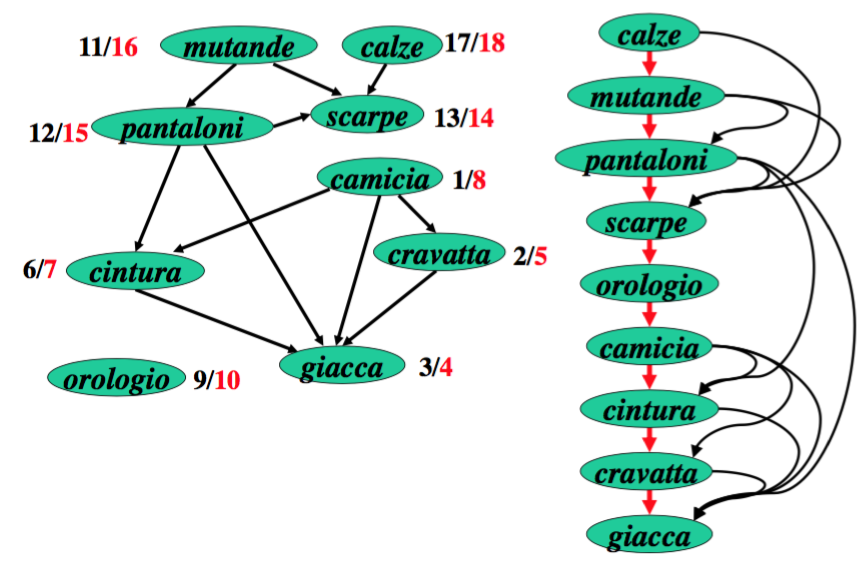
\includegraphics[width=.5\textwidth]{./notes/immagini/l7-fig1.png}
\end{figure}

\section{Un primo modello lineare}\label{un-primo-modello-lineare}

Ipotizzando che ci sia una relazione lineare è possibile utilizzare il
modello del capitolo precedente:

$$
y = \alpha + \beta x + \epsilon
$$

$$
\hat{\beta} = \frac{\cov(X,Y)}{\var(X)} \qquad \hat{\alpha} = \bar{y} - \hat{\beta}\bar{x}
$$

Utilizzando l'ambiente R si ottengono delle informazioni relative all
modello ottenuto:

\begin{verbatim}
lm(formula = gas ~ prezzo)
Residuals:
    Min      1Q  Median      3Q     Max
-40.625 -10.719  -1.136  14.073  38.292
Coefficients:
            Estimate Std. Error t value Pr(>|t|)
(Intercept)  138.561     13.552  10.225 6.34e-09 ***
prezzo        -1.104      0.202  -5.467 3.42e-05 ***
---
Signif. codes:  0 ‘***’ 0.001 ‘**’ 0.01 ‘*’ 0.05 ‘.’ 0.1 ‘ ’ 1
Residual standard error: 20.86 on 18 degrees of freedom
Multiple R-Squared: 0.6241,     Adjusted R-squared: 0.6033
F-statistic: 29.89 on 1 and 18 DF,  p-value: 3.417e-05
\end{verbatim}

Dai dati si può notare che l'indice $ R^2 $ è uguale a 0.62, il che indica un buon andamento lineare.
Inoltre come \textit{p-value} si ottiene un valore molto basso, il che porta a rifiutare l'ipotesi nulla.

Tracciando però i grafici dei residui è possibile osservare c'è una componente indipendente che non è lineare.

\begin{figure}[htbp]
	\centering
	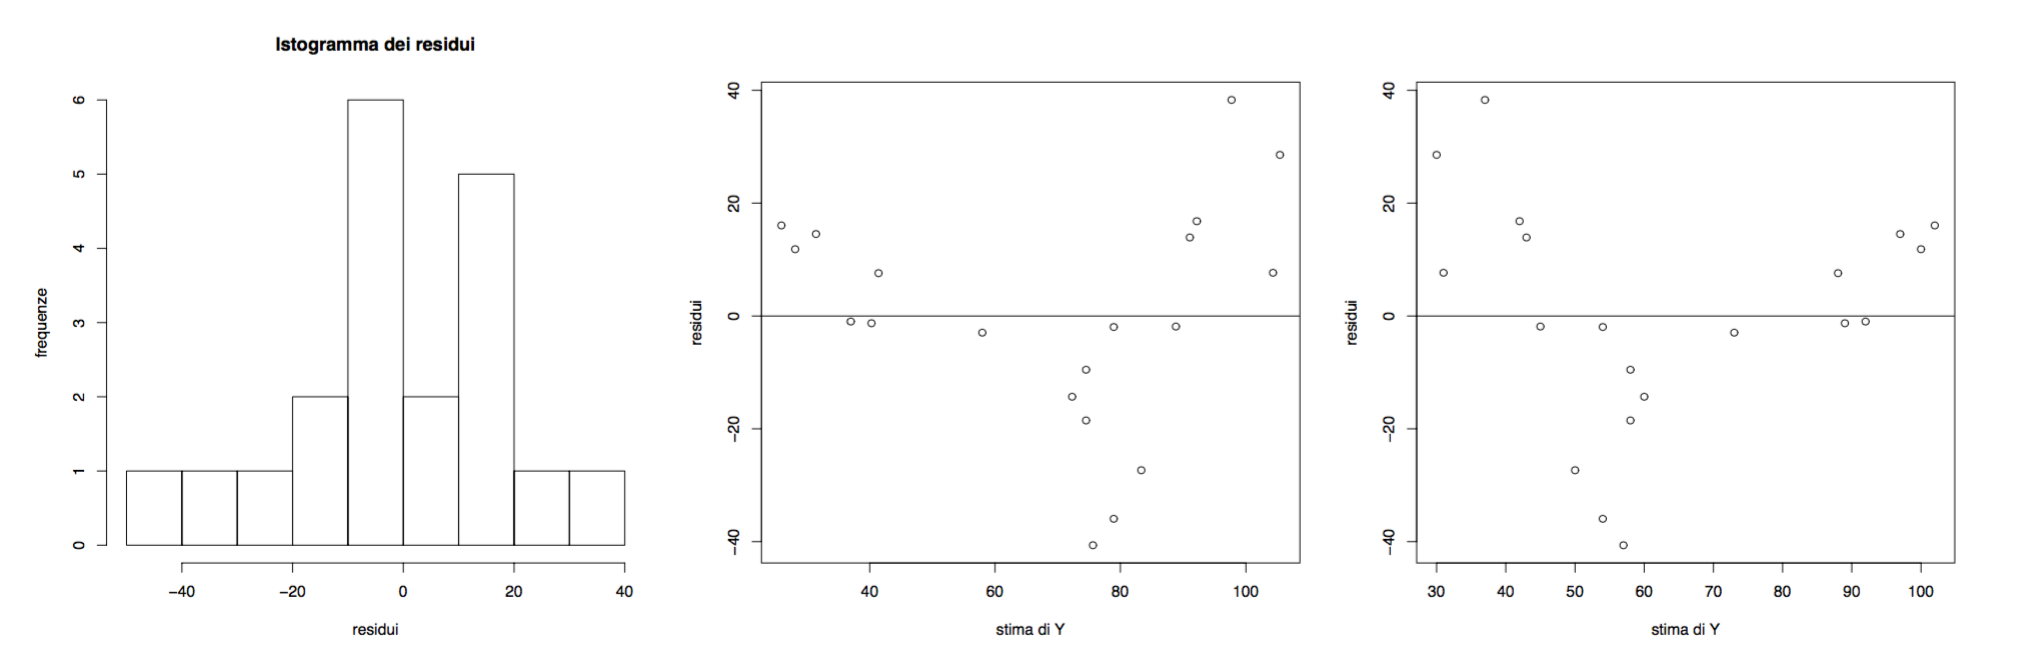
\includegraphics[width=1\textwidth]{./notes/immagini/l7-fig2.png}
	\caption{Tracciamento dei residui per il primo modello. \`{E} possibile notare la presenza di indipendente.}
\end{figure}

\section{Considerazioni sul problema e un secondo modello}\label{considerazioni-sul-problema-e-un-secondo-modello}

Considerando il problema modellato è possibile fare alcune osservazioni:

\begin{itemize}
	\item il consumatore potrebbe destinare solamente un determinato budget $ \kappa $ per l'acquisto del gas, ovvero $ x \cdot y = \kappa $.
	\item è ragionevole pensare che il consumatore debba consumare una quantità minima di gas $ \gamma $
	\item essendo il mercato del gas regolamentato, c'è un prezzo minimo di $ 7 $ centesimi al metro cubo sotto il quale non è possibile vendere il gas.
\end{itemize}

Tenendo in considerazione quanto elencato si arriva ad avere l'equazione:

$$
(x-7)(y-\gamma) = \kappa
$$

la quale può essere riscritta in un modo più simile a quella del modello lineare

$$
y = \gamma + \kappa \cdot \frac{1}{x-7}
$$

e sostituendo la variabile \textit{x} con $ z = \frac{1}{x-7} $, si ottiene proprio la stessa equazione la quale permette di calcolare la retta ai minimi quadrati.

Questo è possibile perché quello che finora è stato chiamato modello lineare è un caso particolare dei \textbf{modelli lineari nei parametri}. Ovvero la limitazione data dalla linearità non riguarda le variabili, ma riguarda solamente i \textbf{parametri} del modello.

Quando viene utilizzato il metodo dei minimi quadrati con questi modelli è necessario tenere in considerazione le trasformazioni che vengono fatte alle variabili, perché i valori calcolati ai minimi quadrati riguardano le variabili trasformate e non quelle di partenza, è necessario quindi \textbf{scalare} in modo opportuno i valori\footnote{Se viene scalata solamente la $ x $ non c'è questo problema perché i minimi quadrati considerano solamente le distanze rispetto l'asse $ y $.}.

La formulazione più generale del modello lineare è quindi

$$
g(y) = \alpha + \beta h(x) + \epsilon
$$

Il modello ottenuto per la nuova formulazione è:
\begin{verbatim}
lm(formula = gas ~ I(1/(prezzo - 7)))
Residuals:
Min    1Q  Median  3Q    Max
-29.617 -4.574 2.394 7.800 30.917
Coefficients:
Estimate Std. Error t value Pr(>|t|) 
(Intercept) 3.918 8.376 0.468 0.646
I(1/(prezzo - 7)) 3034.938 357.037 8.500 1.02e-07 *** 
---
Signif. codes: 0 ‘***’ 0.001 ‘**’ 0.01 ‘*’ 0.05 ‘.’ 0.1 ‘ ’ 1
Residual standard error: 15.19 on 18 degrees of freedom 
Multiple R-Squared: 0.8006, Adjusted R-squared: 0.7895 
F-statistic: 72.26 on 1 and 18 DF, p-value: 1.022e-07
\end{verbatim}

ovvero la retta

$$
y = 3.918 + 3034.938 \cdot \frac{1}{x-7}
$$

\begin{figure}[htbp]
	\centering
	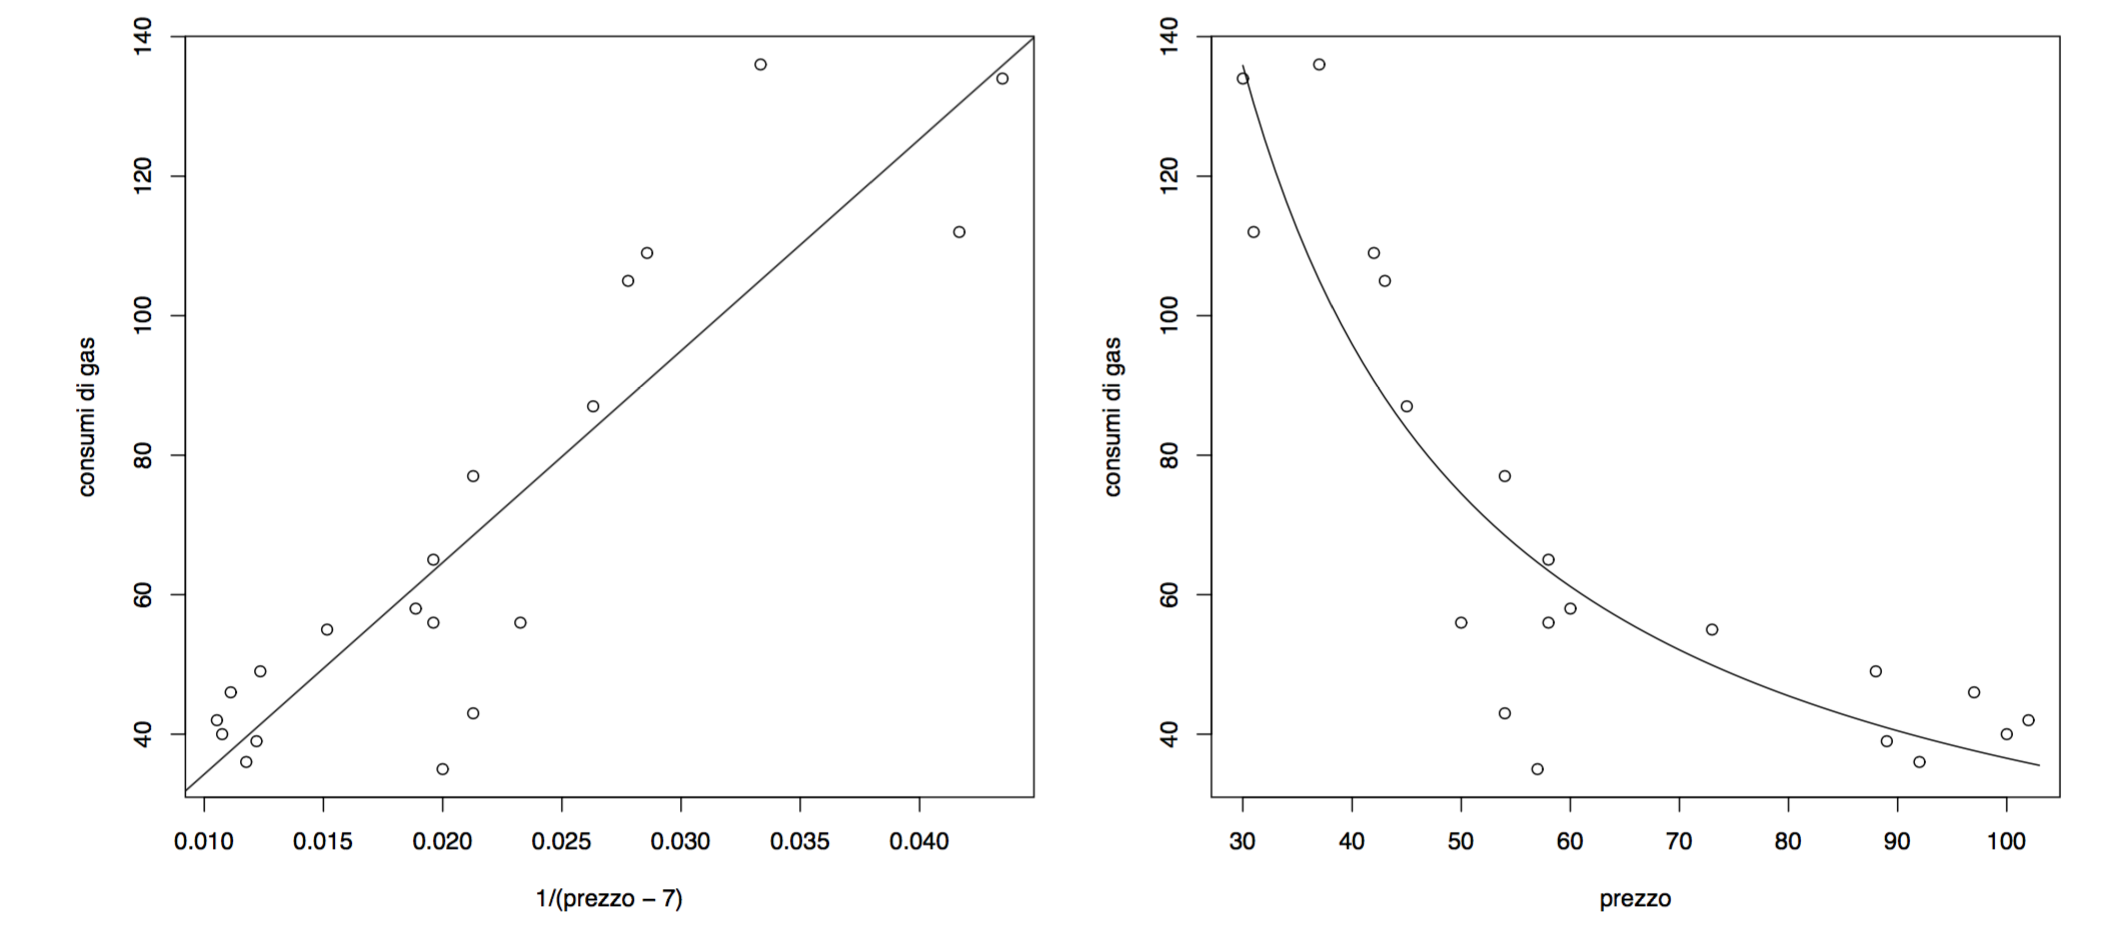
\includegraphics[width=1.1\textwidth]{./notes/immagini/l7-fig3.png}
	\caption{A destra la retta rispetto $ z $. A sinistra il modello lineare tracciato rispetto $ x $.}
\end{figure}

Dai dati del nuovo modello è possibile osservare che la varianza residua (\texttt{Residual standard error} elevato al quadrato) è passata da circa 391 a circa 207, ovvero il quadrato degli errori di previsione è stato ridotto di quasi il $ 50\% $.
Lo stesso effetto può essere visto utilizzando $ R^2 $ che da 0.6241 passa a 0.8006.

\begin{figure}[htbp]
	\centering
	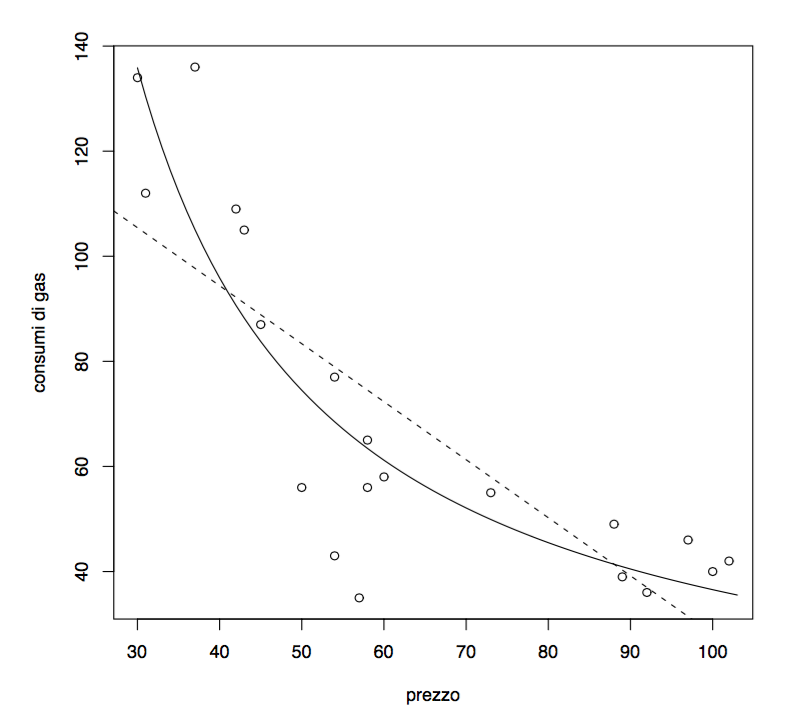
\includegraphics[width=.6\textwidth]{./notes/immagini/l7-fig4.png}
	\caption{Confronto grafico tra i due modelli.}
\end{figure}

\FloatBarrier
\section{Modello lineare con trasformate}\label{modello-lineare-con-trasformate}

\textit{Cambia il dataset di riferimento}, si vuole controllare se il reddito nazionale influisce sulla speranza di vita media dello stato. 

\begin{figure}[htbp]
	\centering
	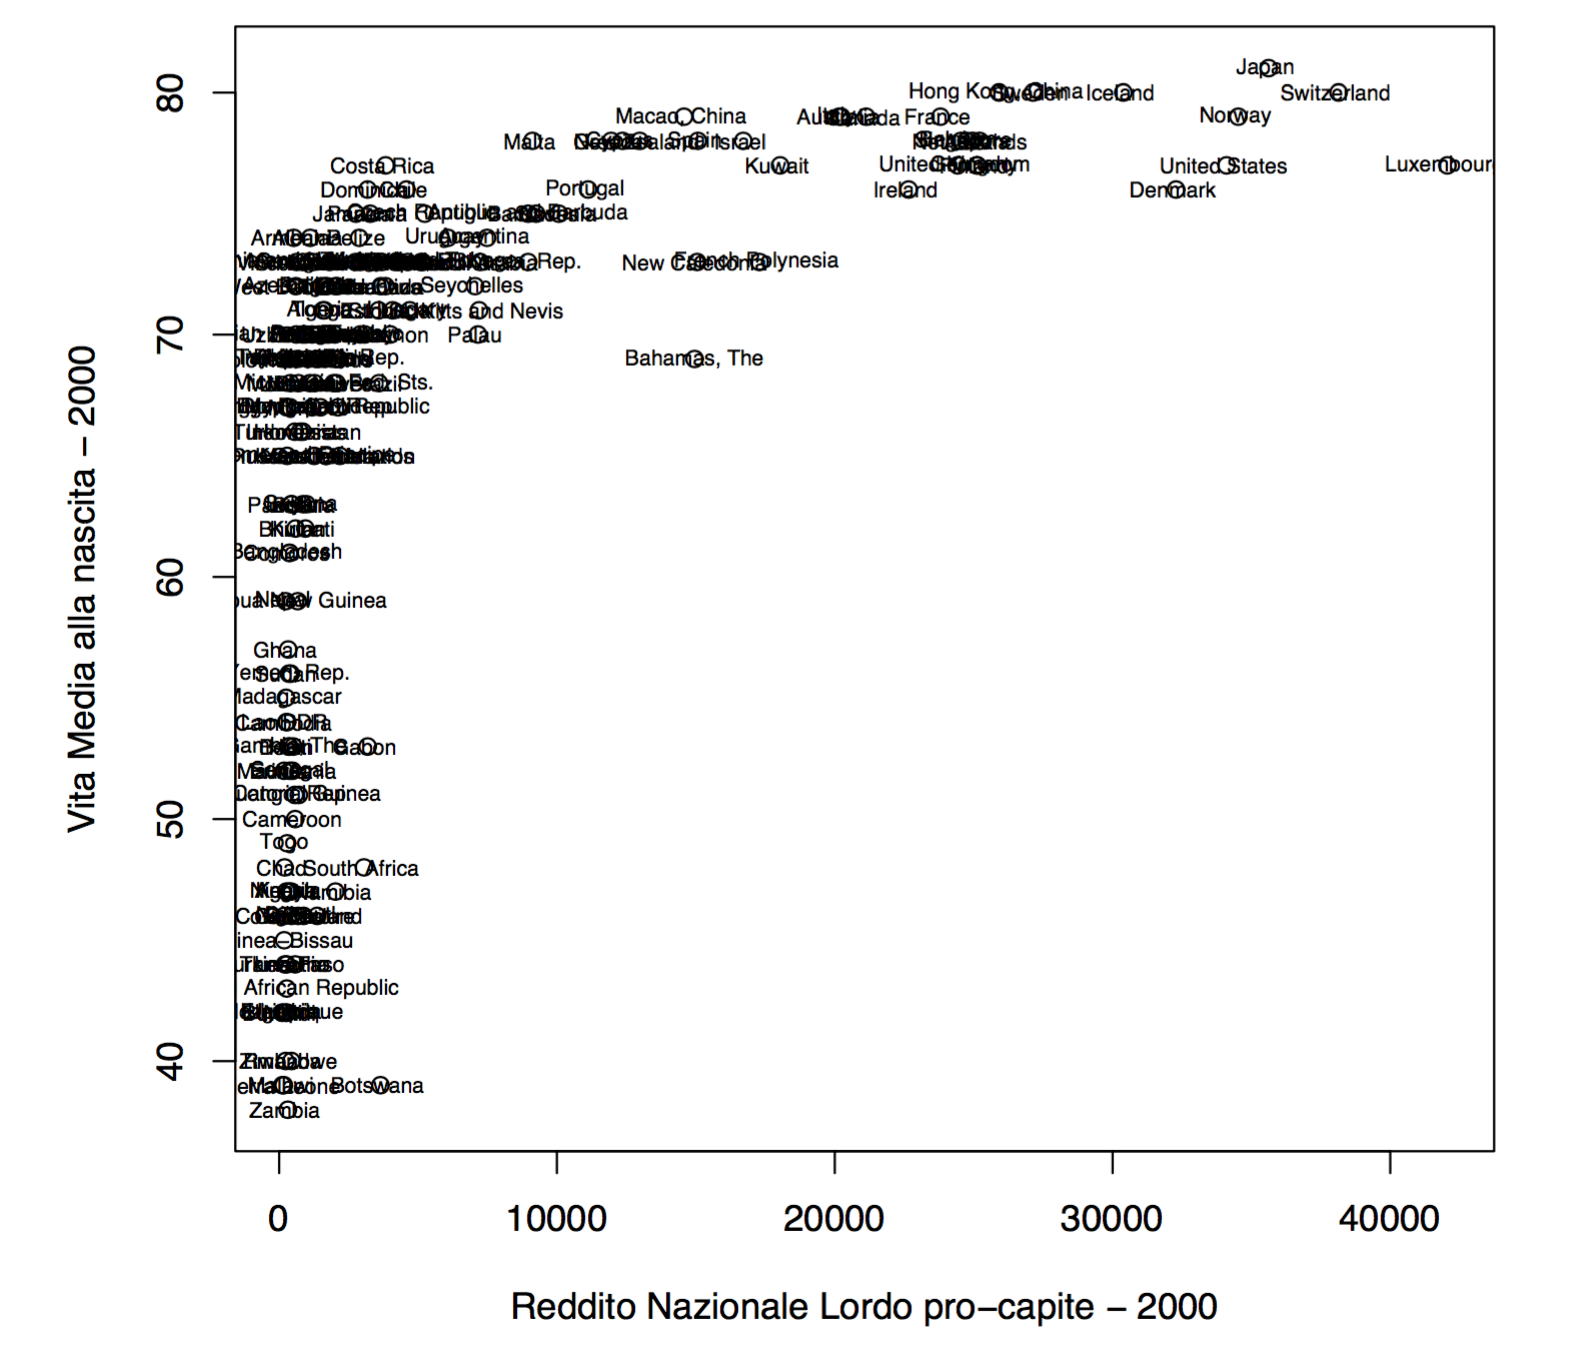
\includegraphics[width=.7\textwidth]{./notes/immagini/l7-fig5.png}
	\caption{Dataset - GNI - ELF}
\end{figure}

La prima cosa da fare è osservare come si comporta il modello lineare senza trasformazioni:

\begin{verbatim}
	lm(formula = elf ~ GNIpc)
	Residuals:
	Min    1Q  Median  3Q    Max
	-24.924 -7.512 4.119 7.431 12.948
	Coefficients:
	Estimate Std. Error t value Pr(>|t|)
	(Intercept) 6.133e+01 8.967e-01 68.390 < 2e-16 ***
	GNIpc 7.115e-04 8.230e-05 8.645 3.76e-15 ***
	---
	Signif. codes: 0 ‘***’ 0.001 ‘**’ 0.01 ‘*’ 0.05 ‘.’ 0.1 ‘ ’ 1
	Residual standard error: 9.903 on 171 degrees of freedom 
	Multiple R-Squared: 0.3041, Adjusted R-squared: 0.3 
	F-statistic: 74.73 on 1 and 171 DF, p-value: 3.757e-15
\end{verbatim}

Si può notare come l'indice $ R^2 $ sia molto basso (0.3041), ma risulta essere molto significativo perché, per il \textit{p-value} ottenuto sia ha che è improbabile che valga l'ipotesi nulla.

Tracciando il modello e il grafico dei residui è possibile notare che
\begin{itemize}
	\item La retta ottenuta non curva abbastanza e quindi non si adatta bene ai dati
	\item Il modello prevede una vita media che può essere maggiore di 90 anni, il che è abbastanza improbabile.
\end{itemize}

\begin{figure}[htbp]
	\centering
	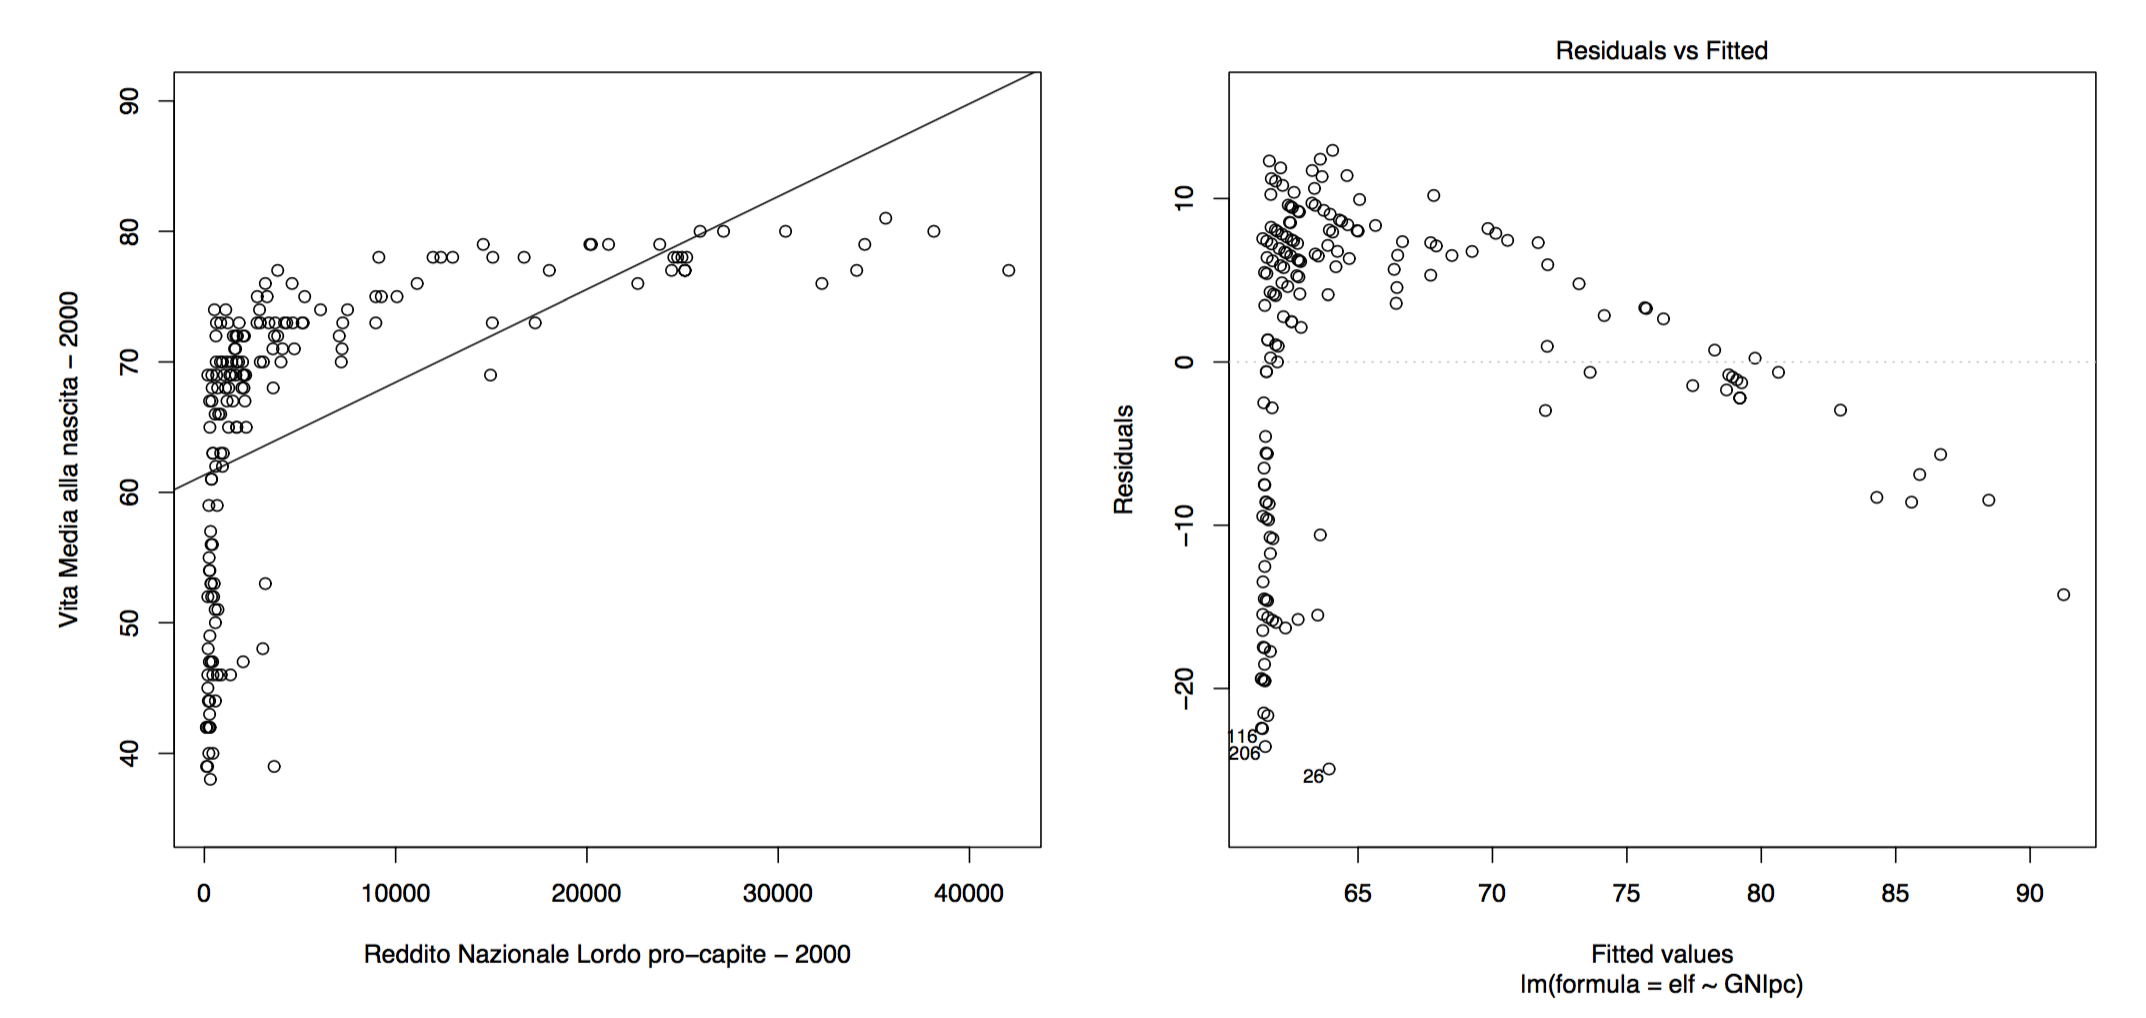
\includegraphics[width=.9\textwidth]{./notes/immagini/l7-fig6.png}
	\caption{Primo modello e residui ottenuti}
\end{figure}

Per adattare meglio la curva è possibile utilizzare la scala logaritmica per l'asse delle \textit{x}. In questo modo, al crescere del reddito viene dato via via meno peso.
Inoltre, rappresentando graficamente questa trasformazioni si ottiene una nuvola di punti più simile ad una retta.

\begin{figure}[htbp]
	\centering
	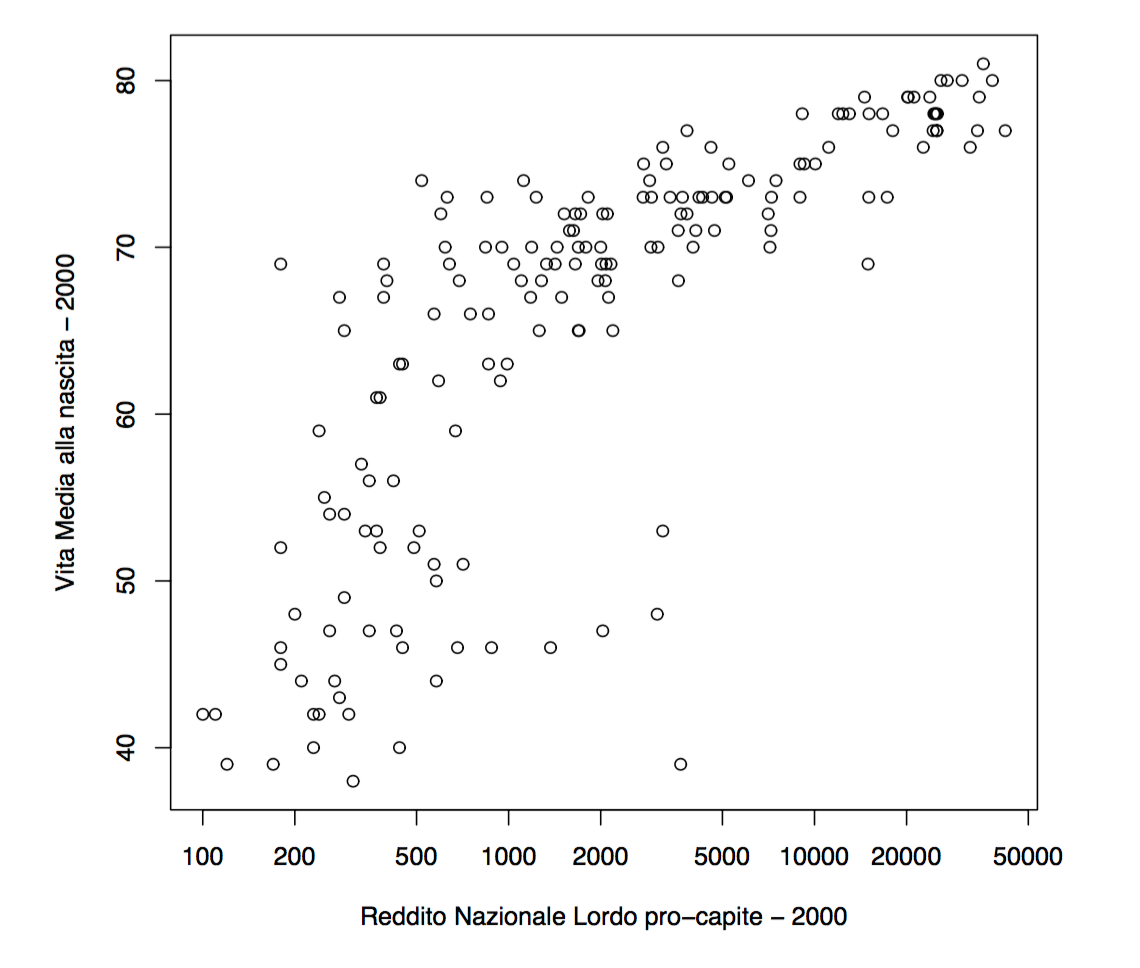
\includegraphics[width=.6\textwidth]{./notes/immagini/l7-fig7.png}
	\caption{Grafico che utilizza la scala logaritmica per i valori delle $ x $. L'asse è comunque etichettato con i valori originali.}
\end{figure}

Il modello diventa quindi

$$
(\text{vita media alla nascita}) = \alpha + \beta \log(\text{reddito nazionale pro capite})
$$

\begin{verbatim}
lm(formula = elf ~ I(logGDP), data = elf.data)
Residuals:
Min     1Q   Median   3Q     Max
-29.6591 -2.9511 0.7906 5.1050 17.4844
Coefficients:
Estimate Std. Error t value Pr(>|t|)
(Intercept) 22.6701 2.8447 7.969 2.02e-13 *** 
I(logGDP) 5.6767 0.3677 15.438 < 2e-16 ***
---
Signif. codes: 0 ‘***’ 0.001 ‘**’ 0.01 ‘*’ 0.05 ‘.’ 0.1 ‘ ’ 1
Residual standard error: 7.674 on 174 degrees of freedom 
Multiple R-Squared: 0.578, Adjusted R-squared: 0.5756 
F-statistic: 238.3 on 1 and 174 DF, p-value: < 2.2e-16
\end{verbatim}

Con questo secondo modello si ottiene un indice $ R^2 $ doppio rispetto al precedente e questo può essere osservato anche nella rappresentazione grafica del nuovo modello.

\begin{figure}[htbp]
	\centering
	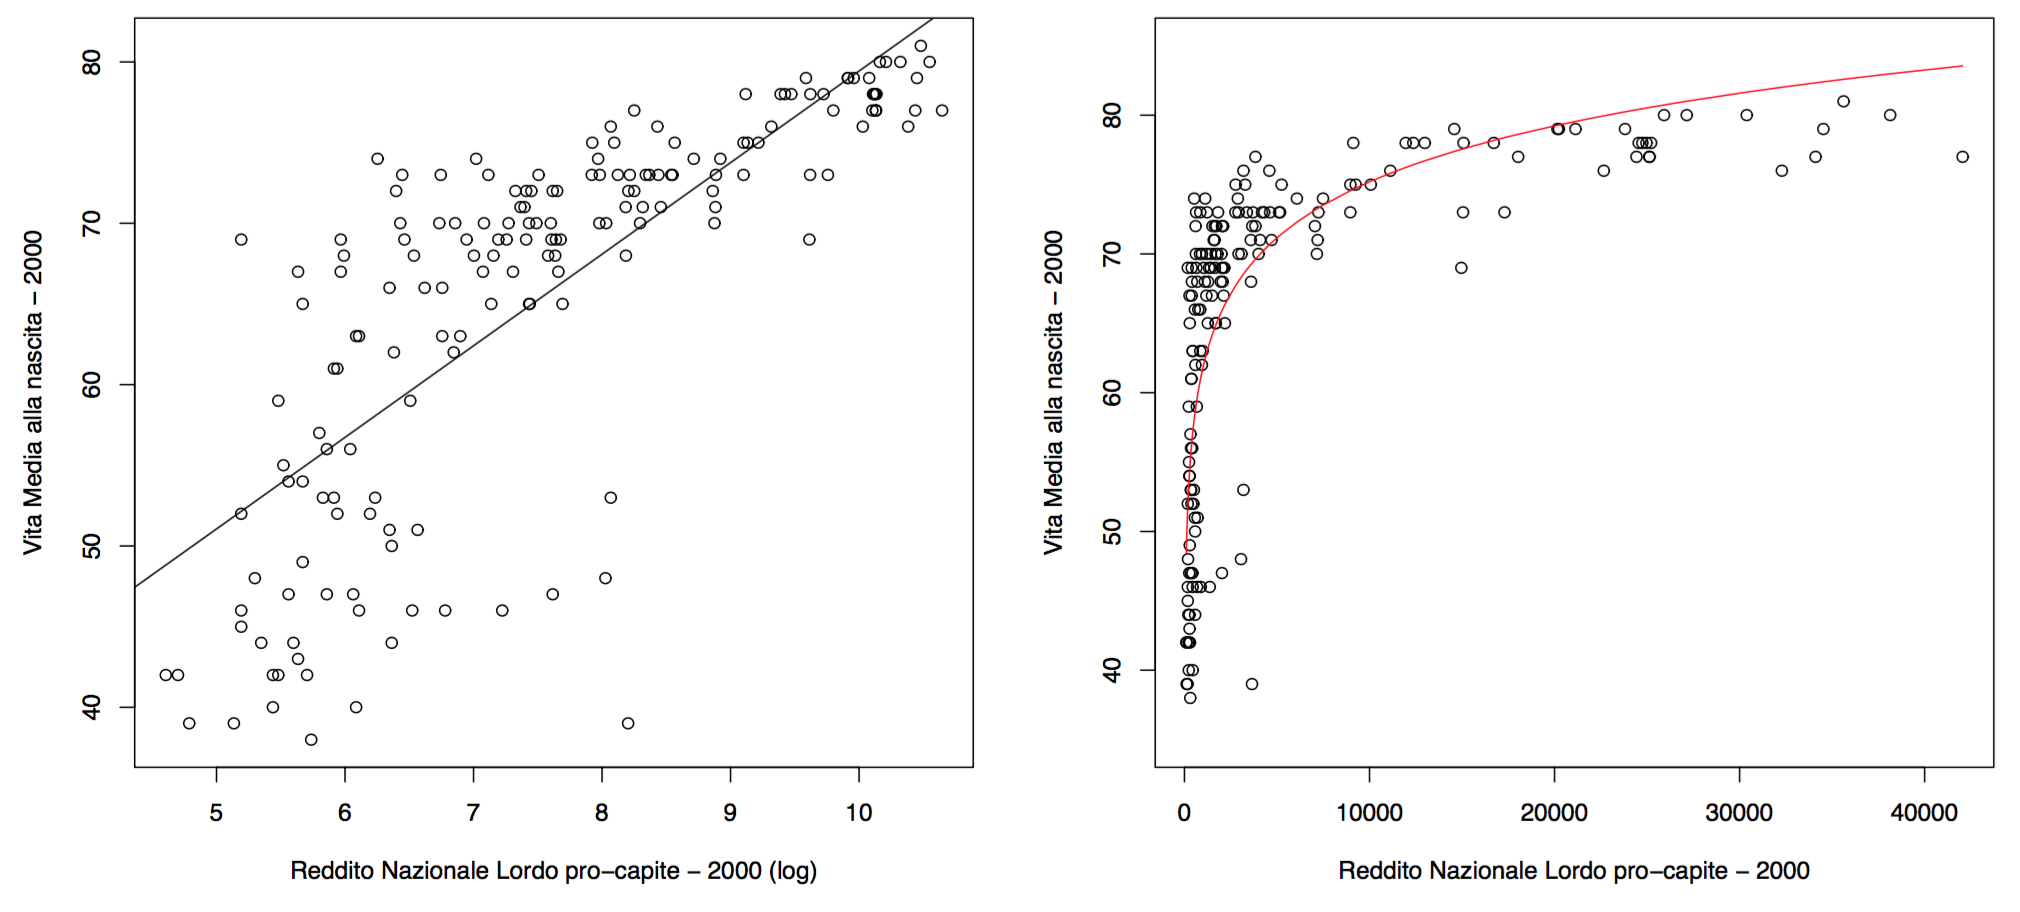
\includegraphics[width=.9\textwidth]{./notes/immagini/l7-fig8.png}
	\caption{Secondo modello: a sinistra con la scala logaritmica, a destra normale.}
\end{figure}

C'è però ancora un problema che riguarda i valori estremi che non vengono approssimati bene dalla curva e lo si può notare anche dai residui.

\begin{figure}[htbp]
	\centering
	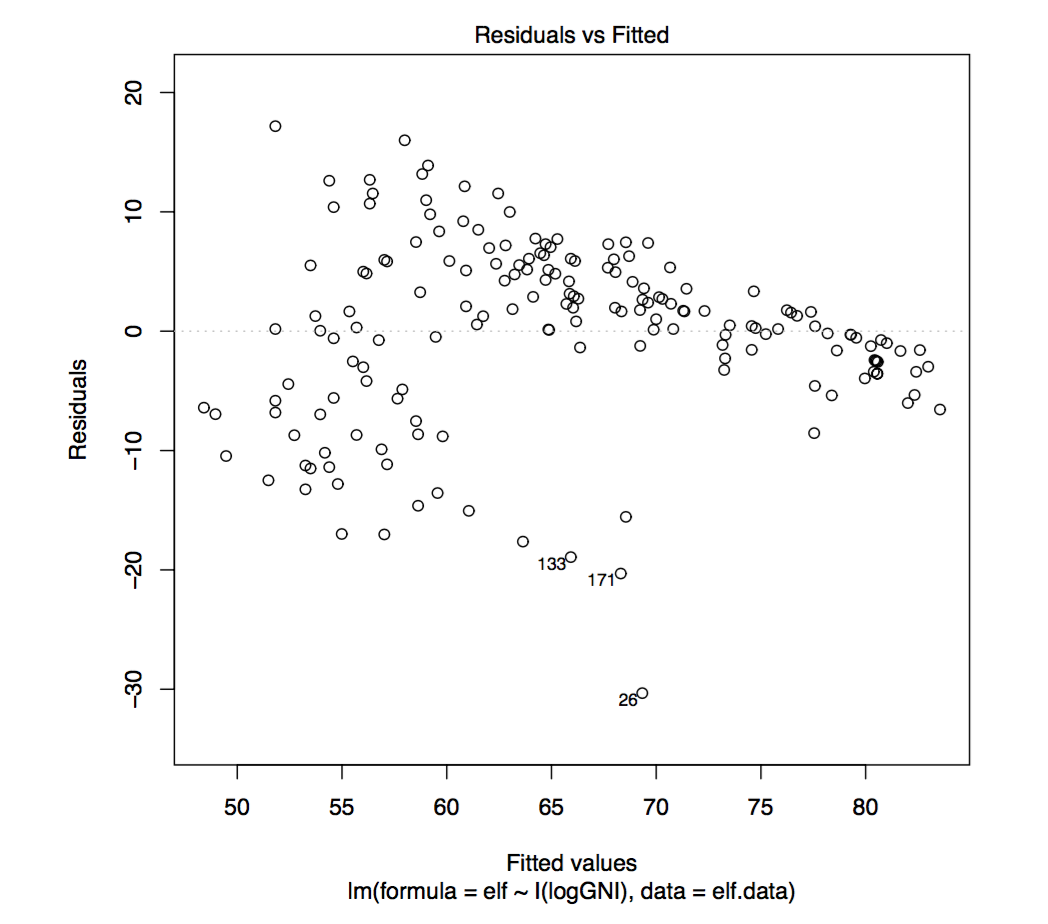
\includegraphics[width=.6\textwidth]{./notes/immagini/l7-fig9.png}
	\caption{Residui per il secondo modello }
\end{figure}

Un'ulteriore modifica può essere quella di trasformare anche la variabile risposta, elevandola alla quinta, in modo da dare maggior peso ai valori maggiori.

Il modello ottenuto è quindi dato da

$$
(\text{vita media alla nascita})^5 = \alpha + \beta \log(\text{reddito nazionale pro capite}) + \epsilon
$$

Da notare che con questa formulazione le ipotesi sugli errori (media nulla, varianza costante, distribuzione normale, ecc.) \textbf{devono valere per gli errori su scala trasformata}.

Una volta calcolato il modello si ottiene

\begin{verbatim}
lm(formula = elf.5 ~ logGNI, data = elf.data)
Residuals:
Min        1Q        Median    3Q       Max
-1.801e+09 -2.817e+08 7.965e+06 3.036e+08 1.334e+09
Coefficients:
Estimate Std. Error t value Pr(>|t|) 
(Intercept) -2.345e+09 1.832e+08 -12.80 <2e-16 *** 
logGNI 5.164e+08 2.376e+07 21.73 <2e-16 ***
---
Signif. codes: 0 ‘***’ 0.001 ‘**’ 0.01 ‘*’ 0.05 ‘.’ 0.1 ‘ ’ 1
Residual standard error: 4.89e+08 on 171 degrees of freedom 
Multiple R-Squared: 0.7341, Adjusted R-squared: 0.7326 
F-statistic: 472.2 on 1 and 171 DF, p-value: < 2.2e-16
\end{verbatim}

\begin{figure}[htbp]
	\centering
	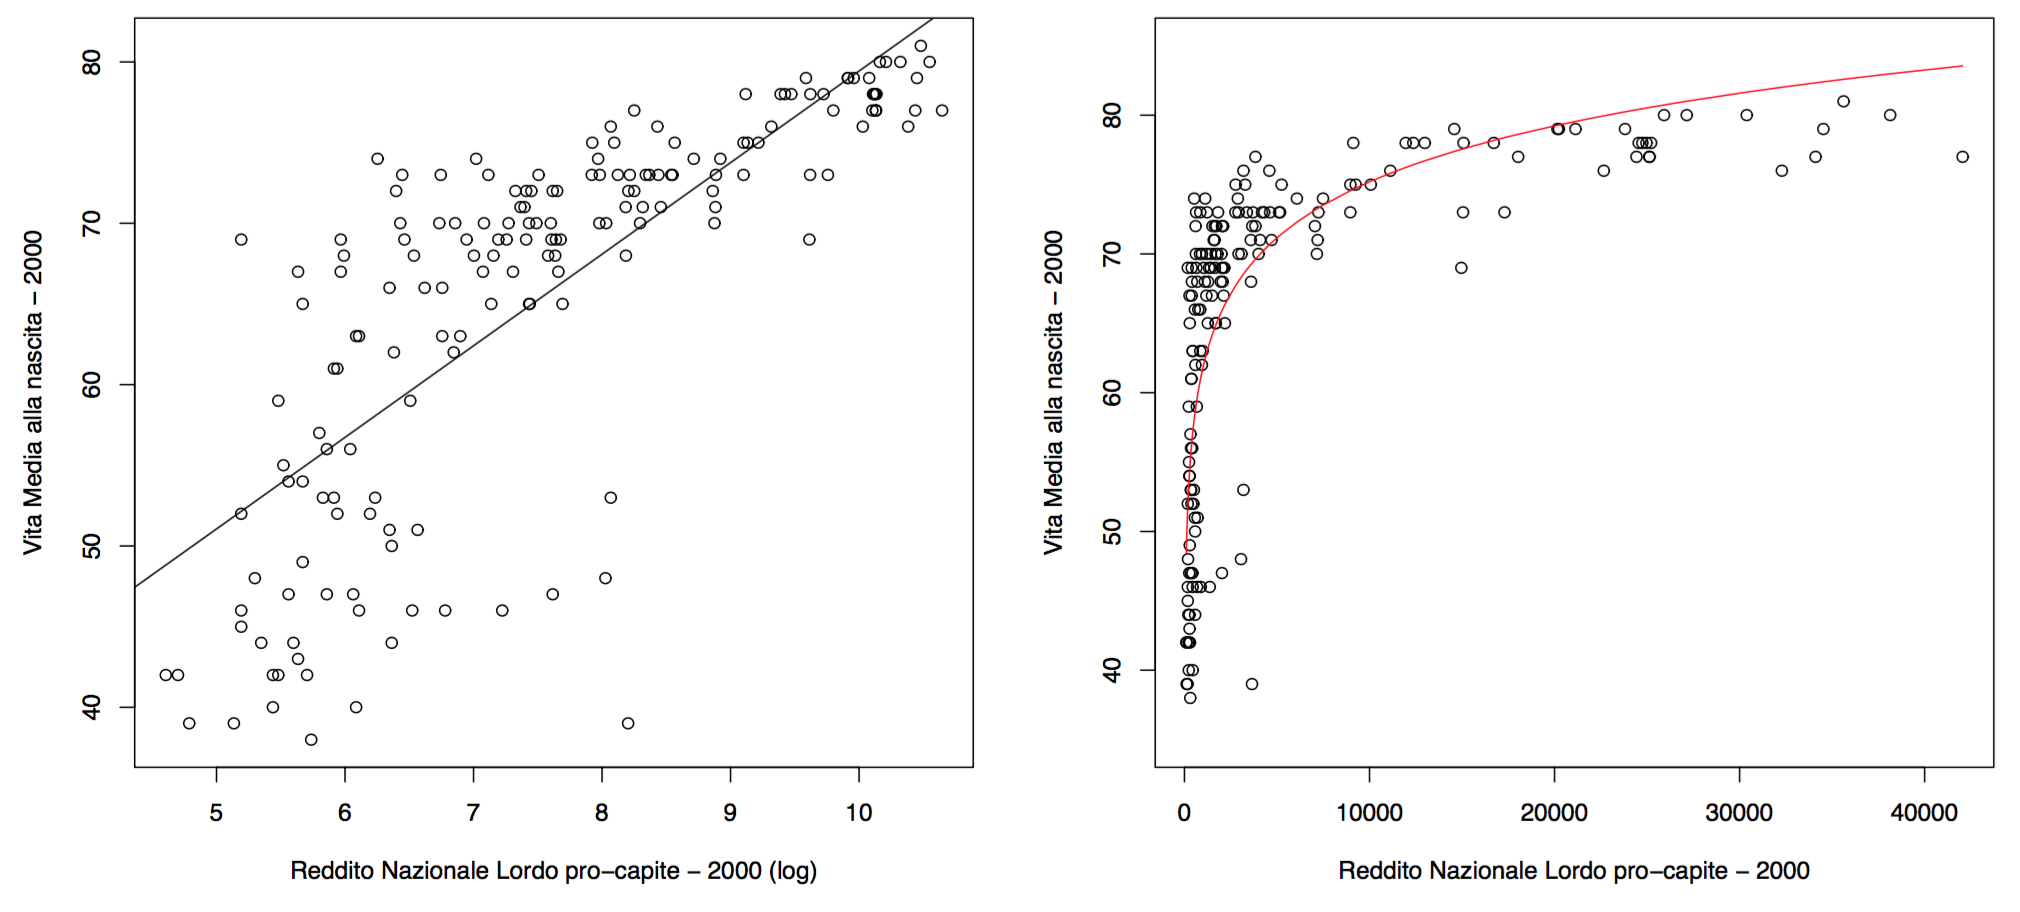
\includegraphics[width=.9\textwidth]{./notes/immagini/l7-fig8.png}
	\caption{Terzo modello: a sinistra con la scala originale e a destra i residui.}
\end{figure}

L'indice $ R^2 $ ottenuto fa riferimento ai residui calcolati sulla scala trasformata, quindi per avere un'indice di adattamento dei dati è possibile utilizzare la media dei quadrati dei residui per la variabile originale:

$$
\frac{1}{n}\sum\limits_{i=1}^n \bigg[ \big(\text{vita media alla nascita}\big)_i - \sqrt[5]{\big(\alpha + \beta \log(\text{reddito nazionale pro capite})_i\big)}\bigg]^2
$$

Calcolando questo valore si ottiene 55.08, mentre con il secondo modello si aveva la varianza dei residui pari a 58.89. Si ottiene quindi una riduzione del $ 6\% $ del quadrato degli errori di previsione.










	% !TEX encoding = UTF-8
% !TEX program = pdflatex
% !TEX root = AALP.tex
% !TEX spellcheck = it-IT

% 27 Ottobre 2016
%\section{Estensioni del nostro linguaggio}
%\subsection{Record}
% \subsubsection{L'oggetto conto}

\section{Tipi variante}

Se i record possono essere visti come tipi congiunzione, che combinano più tipi, i tipi variante possono essere visti come disgiunzione.

Ad esempio possiamo pensare ad un contatto in una rubrica che può avere un indirizzo fisico o virtuale:

$$
< \text{fisico}: \underbrace{\{ \text{nome : String}, \text{indirizzo: String} \}}_{T_{fisico}} , \: \text{virtuale}: \underbrace{\{ \text{login : String}, \text{email : String} \}}_{T_{virt}} >= T_{ind}
$$

\noindent Un esempio di valore che ha questo tipo è:

$$
< \text{fisico} = \{ \text{nome = ``pippo''}, \text{indirizzo =  ``Via rosa''} \} >
$$

\noindent L'utilità di questi tipi si ha con l'operatore di pattern matching.
Ad esempio in Scala è possibile definire delle funzione generiche che lavorano sui tipi variante:

\begin{lstlisting}[language=Scala, caption=Utilizzo del pattern matching in Scala]
def getName(a : Tind) : String = a match{
	case <fisico = x> => x.nome
	case <virtuale = x> => x.login
	/** case <l = x> => ... da errore di compilazione! */
	/** allo stesso modo viene segnalato se il pattern non copre tutte le possibili etichette */
}

def getAll(a : List[Tind] ) : List[String] = {
	var l = new List[String]
	for (x <- a) l.add(getName(x))
}
\end{lstlisting}

\noindent Per inserire nel nostro linguaggio questi valori servono dei nuovi termini:

$$
M ::= < l = M > \vbar M \text{ match } \{\text{case }l_i = x_i => M_i \:^{i = 1\ldots n}\} \vbar \ldots
$$

\noindent Da notare che la $x_i$ che viene utilizzata nel \text{match} lega le eventuali occorrenze all'interno di $M_i$.

$$
<l_1 = 3> \text{ match } \{\text{case } l_1 = x => x+1, \ldots \} \rightarrow 3+1
$$

\noindent Più formalmente:

\begin{itemize}
	\item $fv(<l =M>) = fv(M)$
	\item $fv( M \text{ match } \{\text{case }l_i = x_i => M_i \:^{i = 1\ldots n}\}) = fv(M) \cup \bigcup_{i = 1 \ldots n}\bigg( fv(M_i) \setminus \{x_i\} \bigg) $
\end{itemize}


\noindent Servono inoltre dei nuovi valori finali e dei tipi:

$$
v ::= <l = v> \vbar \ldots \qquad T ::= < l_i : T_i \:^{i = 1 \ldots n}>
$$

\noindent La semantica operazionale viene espressa con 3 nuove regole:

\begin{itemize}
	\item Riduzione del termine interno
	\begin{prooftree}
		\AxiomC{$M \rightarrow M'$}
		\LL{Variant}
		\UnaryInfC{$<l = M> \rightarrow <l = M'>$}
	\end{prooftree}
	\item Avanzamento in un match:
	\begin{prooftree}
		\AxiomC{$M \rightarrow M'$}
		\LL{Red-Match}
		\UnaryInfC{$M \text{ match } \{\text{case } l_i = x_i => M_i \:^{i = 1 \ldots n}\} \to M' \text{ match } \{\text{case } l_i = x_i => M_i \:^{i = 1 \ldots n}\}$}
	\end{prooftree}
	\item Assioma per il match effettivo
	\begin{prooftree}
		\AxiomC{$j \in \{1 \ldots n\}$}
		\LL{Match}
		\UnaryInfC{$<l_j = v> \text{ match } \{\text{case } l_i = x_i => M_i \:^{i = 1 \ldots n}\} \rightarrow M_j\{x_j = v\}$}
	\end{prooftree}
\end{itemize}

\noindent Servono inoltre delle regole di tipo, una per l'invariante e l'altra per il match.

\begin{prooftree}
	\AxiomC{$ \Gamma \vdash M: T_j $}
	\AxiomC{$ j \in \{1 \ldots n \} $}
	\LL{Type-Variant}
	\BinaryInfC{$\Gamma \vdash <l_j = M> : <l_i : T_i \:^{i=1\ldots n}>$}
\end{prooftree}

\noindent Con questa regola posso assegnare ad un valore infiniti tipi, l'importante è che in questi infiniti tipi ci sia l'etichetta $l_j$ in modo da avere la garanzia di riuscire ad effettuare il pattern matching.

\begin{prooftree}
	\AxiomC{$\Gamma \vdash M : < l_i : T_i  \:^{i=1\ldots n}>$}
	\AxiomC{$\Gamma, x_i : T_i \vdash M_i : T \:\: \forall \: i = 1 \ldots n $}
	\LL{Type-Match}
	\BinaryInfC{$\Gamma \vdash M \text{ match }\{\text{case }l_i = x_i => M_i \:^{i=1\ldots n}\} : T$}
\end{prooftree}

\noindent Perché un match sia ben tipato è necessario che il termine $M$ sia un valore di tipo variante e che tutti i ``rami'' del match siano termini con lo stesso tipo, aggiungendo anche al contesto la sostituzione che viene effettuata quando viene applicato il match.

Se nel pattern matching ho come premessa della regola $\Gamma \vdash M : < l_i : T_i  \:^{i=1\ldots m}>$ con $m \geq n$ c'è un problema perché possono capitare delle etichette che il costrutto \text{match} non riesce a gestire. Se invece $m \leq n$ non ci sono problemi. Ma anche in questo caso, dato che ho a disposizione infiniti tipi, conviene forzare $m = n$.

Anche se non sembra questi tipi sono presenti nella maggior parte dei linguaggi main stream, solo che questi vengono nascosti da dello zucchero sintattico. Ad esempio le liste possono essere viste come un tipo variante in quanto sono o una lista vuota o la concatenazione di un elemento e un'altra lista.

$$
\text{List} = < \text{nil : Unit}, \text{cons} : (\Nat * \text{List}) >
$$

\noindent Si tratta di un tipo ricorsivo che non è supportato nella nostra grammatica, ma in altre grammatiche è possibile gestirlo.

I valori per questo tipo sono:

$$
<\text{nil } = \text{unit}>  \quad <\text{cons} = (5, <\text{nil } = \text{unit}>)>
$$

\noindent Un altro caso d'uso dei valori variante è l'analisi delle dereferenziazioni dei valori null.
Ad esempio in Java possiamo definire una variabile e assegnarle null:

\begin{lstlisting}[language=Java]
C c = null;

C find(List<C> l, C a) { ... } // se non trova ritorna null

C c = find(list, s);
// c può essere null, quindi devo controllare
// se non controllo potrei finire in un NullPointerException, anche perché il compilatore non controlla questo tipo di eccezioni
if (c != null) print(c.info());
else print("non trovato");
\end{lstlisting}

\noindent Questo approccio non è dei migliori, perché dovrebbe utilizzare le eccezioni personalizzate, ma si è visto che nessuno le usa. Con C\# si sono invece inventati i tipi \texttt{Nullable} che possono avere anche come valore \texttt{Null}, anche per i tipi primitivi.

Un'altra idea è stata quella di introdurre i tipi \texttt{!}: una classe di tipo \texttt{C!} non può assumere come valore null, in modo da sfruttare di più l'analisi statica.

Linguaggio che vai, soluzione che trovi. Altri linguaggi utilizzano i così detti \textbf{null objects}:

\begin{lstlisting}[language=Java]
class C {
	...
	String info() {...}
	...
}
class NullC extends C {
	...
	String info() {}
}
\end{lstlisting}

\noindent Così facendo c'è un metodo definito da chiamare anche sul valore null, in modo da evitare la NullPointerExcpetion.

Scala e Java8 (e Swift) implementano un'ulteriore versione, gli \textbf{option type}, ovvero un tipo variante che prevede due possibilità: c'è l'oggetto oppure non c'è.
La definizione di questo tipo è la seguente:

$$
Option[C] = < \text{none} : \text{Unit}, \text{some} : C >
$$

\noindent Il codice di prima può essere quindi riscritto come

\begin{lstlisting}[language=Scala]
...
def find(l : List[C], s : String) : Option[C] = {
	for(x <- l) 
		if (x.info() == s) return Some(x)
	return None 
}
...
find(l, "pippo") match {
	case Some(x) => print(x.info())
	case None => print("non trovato")
}
\end{lstlisting}

\noindent Si può notare come questa versione del codice è più espressiva e si riesce subito a capire che la funzione \texttt{find} può non trovare l'elemento cercato.



	% !TEX encoding = UTF-8
% !TEX TS-program = pdflatex
% !TEX root = computabilità e algoritmi.tex
% !TEX spellcheck = it-IT
\section{Composizione generalizzata}\label{composizione-generalizzata}

$$f: \mathbb{N}^k \rightarrow \mathbb{N},\: g_1,\ldots g_n : \mathbb{N}^k \rightarrow \mathbb{N}$$

La loro composizione $h: \mathbb{N}^k \rightarrow \mathbb{N}$ è data da: 

$$
h(\vec{x}) = f(g_1(\vec{x}), \ldots, g_n(\vec{x}))
$$

La funzione $h(\vec{x})\downarrow$ (è definita) se tutte le
$g_i \downarrow y_i, f(y_1,\ldots,y_n) \downarrow$.

L'approccio utilizzato nella valutazione delle funzioni è quello
\textbf{eager}, ovvero vengono valutati prima tutti i parametri.

Ad esempio: $\underline{0} : \mathbb{N} \rightarrow \mathbb{N},\: \underline{0}(x) = 0$ e $d(x) = \uparrow,\: \underline{0}(d(1))$ è
$\uparrow$ perché prima è necessario valutare i parametri.

\subsection{Calcolabilità della funzione
composta}\label{calcolabilituxe0-della-funzione-composta}

Se $f: \mathbb{N}^n \rightarrow \mathbb{N}, g_1\ldots g_n : \mathbb{N}^k \rightarrow \mathbb{N} \in \mathcal{C}$, allora anche $h: \mathbb{N}^k \rightarrow \mathbb{N}$ è calcolabile in $\mathcal{C}$.

\subsubsection{Dimostrazione}\label{dimostrazione}

Siano $F,G_1, \ldots{}, G_n$ programmi URM in forma normale per
le relative funzioni.

L'input della funzione \emph{h} avrà nei primi \emph{k} registri i
valori di input, è necessario quindi andare a copiarli in una locazione
di memoria che non viene usata dai vari programmi, ovvero dalla
locazione \emph{m+1}, con $m = max\{\rho(F), \rho(G_1), \ldots \rho(G_N), k,n\}$.

I risultati parziali dei programmi vengono poi memorizzati a partire
dalla locazione \emph{m + k +1} per poi essere utilizzati da \emph{F}

Il programma risultante è:

\begin{lstlisting}[language=URM]
T([1 ... k],[m+1 ... m+k])
G1[m+1 ... m+k -> m+k+1]
...
Gn[m+1 ... m+k -> m+k+n]
F[m+k+1 ... m+k+n -> 1]
\end{lstlisting}

\subsubsection{Esempio - Somma di due numeri}\label{esempio}

A partire dalla funzione $sum(x_1, x_2) = x_1+x_2$ è possibile andare a ottenere la funzione

$$f(x_1, x_2, x_3) = x_1 + x_2 +x_3$$

componendo la funzione \textit{sum} con se stessa:

$$f(x_1, x_2, x_3) = sum(sum(x_1,x_2),x_3)$$

Tuttavia, strettamente parlando, le $g_i$ non hanno la stessa
arietà, pertanto sono necessari dei piccoli aggiustamenti:

$$f(x_1, x_2, x_3) = sum(sum(U_1^{3}(\vec{x}),U_2^3(\vec{x}))), U_3^3(\vec{x}))$$

\section{Ricorsione Primitiva}\label{ricorsione-primitiva}

\begin{align*}
	fact(0) &= 1 \\
	fact(n+1) &= (n+1)fact(n)
\end{align*}

\begin{align*}
	fib(0) &= 1 \\
	fib(1) &= 1 \\
	fib(n+2) &= fib(n+1) + fib(n)
\end{align*}

Date $f: \mathbb{N}^k \rightarrow \mathbb{N}$ e $g:\mathbb{N}^{k+2} \rightarrow \mathbb{N}$, la funzione per ricorsione primitiva $h: \mathbb{N}^{k+1} \rightarrow \mathbb{N}$ è definita come

\begin{align*}
	h(\vec{x}, 0) &= f(x) \\
	h(\vec{x}, y+1) &= g(\vec{x}, y, h(\vec{x},y))
\end{align*}

Così facendo viene definita \emph{h} utilizzando \emph{h} e
concettualmente è corretto, tuttavia è necessario dimostrare formalmente
l'esistenza e l'unicità di \emph{h}.

Questo lo si fa considerando l'operatore $\Phi$:

\begin{align*}
	\Phi : (\mathbb{N}^k \rightarrow \mathbb{N}) &\rightarrow (\mathbb{N}^k \rightarrow \mathbb{N}) \\
	\Phi(h)(\vec{x}, 0) &= f(\vec{x}) \\
	\Phi(h)(\vec{x}, y+1) &= g(\vec{x}, y, h(\vec{x},y))
\end{align*}

tale che $\Phi(h) = h$, ovvero tale che viene raggiunto un punto
fisso. Ciò sarebbe da dimostrare, ma questo va oltre l'obiettivo del corso, quindi viene dato per buono.

In altre parole, se \emph{h} rispetta lo schema precedentemente definito, allora esiste ed è unica.

Assumendo quindi che la ricorsione primitiva di una funzione calcolabili
è calcolabile, è possibile definire varie operazioni senza scrivere
esplicitamente il programma per calcolarle:

Ad esempio la funzione somma può essere definita in modo ricorsivo:

$$
	x+y = h(x,y) =\begin{cases}
	x+0 = x &\Rightarrow f(x) = x \\
	x+(y+1) = (x+y) + 1 &\Rightarrow g(x,y,z) = succ(z)
	\end{cases}
$$

In modo simile possono essere anche definiti il prodotto e l'esponenziale:

$$
x \cdot y = h(x,y) =\begin{cases}
x \cdot 0 = 0 &\Rightarrow f(x) = 0 \\
x \cdot (y+1) = (x \cdot y) + x &\Rightarrow g(x,y,z) = z+x
\end{cases}
$$

$$
x^y = h(x,y) =\begin{cases}
x^0 = 1 &\Rightarrow f(x) = 1 \\
x^{(y+1)} = (x^y) \cdot x &\Rightarrow g(x,y,z) = z \cdot x
\end{cases}
$$

\subsection{Calcolabilità della Ricorsione Primitiva}\label{calcolabilituxe0-della-ricorsione-primitiva}

Siano $f:\mathbb{N}^k \rightarrow \mathbb{N}$ e $g:\mathbb{N}^{k+2} \rightarrow \mathbb{N} \in \mathcal{C}$ allora anche \emph{h} definita per
ricorsione primitiva è in $\mathcal{C}$. Ovvero quello che è stato assunto precedentemente.

\subsubsection{Dimostrazione}\label{dimostrazione-1}

Siano \emph{F} e \emph{G} i programmi che calcolano \emph{f} e \emph{g}.

Il programma che calcola \emph{h} verrà invocato con il vettore \emph{x}
nelle prime \emph{k} locazioni e con \emph{y} nella locazione
\emph{k+1}.

Come prima cosa è necessario trasferire i dati di input in una zona di
memoria non utilizzata dai programmi \emph{F} e \emph{G}, ovvero
\emph{m+1}, dove $m = max\{\rho(F), \rho(G), k+2\}$.

Dopodiché è necessario effettuare un'interazione su un contatore
\emph{i} che parte da 0, fino a quando non viene raggiunto \emph{y}.

\begin{verbatim}
h(vec(x), 0) = f(vec(x)) -- i=0 -- i==y? NO
h(vec(x), 1) = g(vec(x), 0, h(vec(x),0)) -- i=1 -- i==y? NO
...
h(vec(x), i+1) = g(vec(x), i, h(vec(x),i)) -- i=n -- i==y? SI -> fine
\end{verbatim}

ovvero il programma per \emph{h} sarà:

\begin{lstlisting}[language=URM]
T([1..k], [m+1 ... m+k]) // copia x
T(k+1, m+k+3) //copia y
F[m+1 ... m+k -> m+k+2]
J(m+k+3, m+k+1, END) #LOOP
G[m+1 ... m+k+2 -> m+k+2] // h(vec(x),i+1)
S(m+k+1) //i++
J(1,1,LOOP)
T(m+k+2,1) #END
\end{lstlisting}

Se \emph{f} e \emph{g} sono funzioni parziali quanto dimostrato richiede
maggiori precisazioni, ma a noi basta sapere che se durante il calcolo
troviamo qualche funzione non definita, anche \emph{h} non è definita.

\subsection{Funzioni totali definite ricorsivamente}\label{osservazione-senza-titolo}

Le funzioni definite a parte da funzioni totali mediante composizione o
ricorsione sono anche loro totali.

La dimostrazione per le funzioni mediante composizione è vera per
definizione, l'altra è lasciata per esercizio (si fa per induzione).

\todo[inline]{todo}

\subsection{Esercizio - Libreria di funzioni calcolabili}\label{esercizio---libreria-di-funzioni-calcolabili}

\begin{itemize}
\item
  somma \emph{x+y}
\item
  prodotto $x \cdot y$
\item
  esponenziale $x^y$
\item
  fattoriale \emph{fact(x)}
\end{itemize}

Sguardo d'insieme: vogliamo trovare un programma URM in grado di
simulare un altro programma URM, le operazioni numeriche sono
interessanti perché il programma in input verrà rappresentato come un
numero.

\subsubsection{Predecessore}\label{predecessore}

$$ \text{pred}(x) = \begin{cases}x \dotminus 1 = 0, \:& \text{ se } x=0\\
x-1, \:& \text{ se } x > 0\end{cases}$$

Può essere calcolata ricorsivamente con

\begin{align*}
	0 \dotminus 1 &= 0 \\
	(y+1) \dotminus 1 &= y
\end{align*}

\subsubsection{Sottrazione tra numeri naturali}\label{sottrazione-tra-numeri-naturali}

$$x \dotminus y =\begin{cases}
0,\:& \text{se } x \leq y\\
x-y, \:& \text{altrimenti}
\end{cases}$$

Può essere calcolata ricorsivamente con:

\begin{align*}
x \dotminus 0 &= x \\
x\dotminus (y+1) &= (x \dotminus y) \dotminus 1
\end{align*}

\subsubsection{Segno}\label{segno}

$$sg(x) =\begin{cases}
0,\:& \text{se } x = 0\\
1, \:& \text{altrimenti}
\end{cases}$$

Può essere calcolata ricorsivamente con:

\begin{align*}
sg(0) &= 0 \\
sg(y+1) &= 1
\end{align*}

In modo simile può essere definito anche $\overline{sg}$.

\subsubsection{Valore assoluto della differenza}\label{valore-assoluto-della-differenza}

$$|x - y|=\begin{cases}
x-y,\:& \text{se } x \leq y\\
y-x, \:& \text{altrimenti}
\end{cases}$$

Può essere calcolata in modo composizionale con:

$$|x - y| = (x \dotminus y) + (y \dotminus x)$$


\subsubsection{Minimo}\label{minimo}

$$ \min (x,y) =\begin{cases}
x,\:& \text{se } x \leq y\\
y, \:& \text{altrimenti}
\end{cases}$$

Può essere calcolata con:

$$\min(x,y) = x \dotminus (x \dotminus y)$$

Questo perché se \emph{x} è il minimo, $x\dotminus y$ è 0.

\subsubsection{Resto della divisione intera}\label{resto-della-divisione-intera}

$$\text{rm}(x,y) =\begin{cases}
y \mod x,\:& \text{se } x \neq y\\
y, \:& \text{altrimenti}
\end{cases}$$


Può essere calcolato ricorsivamente come:

\begin{align*}
\text{rm}(x,0) &= 0 \\
\text{rm}(x, y+1) &= \begin{cases}\text{rm}(x+y) +1, \:& \text{ se rm}(x+y) +1 \neq x\\
0, \:& \text{ altrimenti} \end{cases}
\end{align*}

L'\emph{if} può essere espresso in modo algebrico utilizzando la
funzione \emph{sg}, ottenendo:

$$\text{rm}(x, y+1) = (sg(x \dotminus \text{rm}(x,y) \dotminus 1))(\text{rm}(x,y)+1)$$

\subsubsection{Esercizio - Divisione intera}\label{esercizio---divisione-intera}

$$\text{qt}(x,y) =\begin{cases}
\floor[\Big]{\frac{y}{x}},\:& \text{se } x \neq y\\
y, \:& \text{altrimenti}
\end{cases}$$

\todo[inline]{todo}

\subsubsection{Esercizio - Definizione per casi}\label{esercizio---definzione-per-casi}

$f_1 \ldots f_n : \mathbb{N}^k \rightarrow \mathbb{N}$ totali e calcolabili e
$Q_1, \ldots, Q_n \subseteq \mathbb{N}^k$ decidibili e tali che per ogni $\vec{x}$ solo un predicato è vero.

Definire $f(x) = f_1(x) \text{ se } Q_1(x) \ldots f_n(x) \text{ se } Q_n(x)$

\todo[inline]{todo}
 % Modello probabilistico
	% !TEX encoding = UTF-8
% !TEX TS-program = pdflatex
% !TEX root = computabilità e algoritmi.tex
% !TEX spellcheck = it-IT
\chapter{Algoritmi su stringhe}\label{algoritmi-su-stringhe}

\section{Il problema del matching esatto}\label{il-problema-del-matching-esatto}

Si ha un pattern \emph{P} di lunghezza \emph{m} e un testo \emph{T} in
cui cercare il pattern di lunghezza $n \geq m$.

Un esempio di problema è la ricerca del pattern \emph{P = aba} in
\emph{T=bbabaxababay}. In questo caso ci sono 3 occorrenze del pattern,
che si sovrappongono tra loro.

Risolvere questo problema in modo efficiente è di importanza chiave dal
momento che tutti i motori di ricerca si basano sul pattern matching
esatto o approssimato. Un altro campo in cui è utile il pattern matching
è nella bioinformatica, infatti, il DNA umano può essere visto come una
stringa di 4 miliardi di caratteri.

\subsection{Notazione utilizzata}\label{notazione-utilizzata}

Una stringa è composta da un insieme $\Sigma$ di simboli
distinguibili e che prendono il nome di \textbf{caratteri dell'alfabeto}.

L'alfabeto, ovvero l'insieme di simboli, può essere finito oppure
infinito ed è dotato di un ordine totale tra i vari simboli.

Una successione finita dei caratteri dell'alfabeto prende il nome di
\textbf{stringa} e i caratteri che la compongono vengono indicizzati a
partire da 1.

$$
X = x_1 \ldots x_n
$$

$|X|$ indica la lunghezza di una stringa e nel
caso questa sia 0, la stringa è vuota e viene rappresentata con
$\epsilon$.

Due stringhe possono essere concatenate tra loro:

$$
X \cdot Y = x_1\ldots x_ny_1\ldots y_m
$$

e $\epsilon$ è l'elemento neutro per la concatenazione, dal momento
che la concatenazione della stringa vuota ad un'altra stringa è uguale
alla stringa di partenza.

La concatenazione multipla della stessa stringa viene indicata con
l'esponenziale:

$$
X^k = \underbrace{X \cdot \ldots \cdot X}_{k}
$$

Una \textbf{sottostringa} di una stringa \emph{X} è una stringa
\emph{Y}, tale che
$X = Z \cdot Y \cdot W$ per
qualche \emph{Z, W}.

Ogni terna \emph{(Z,Y,W)} prende il nome di \textbf{occorrenza} di
\emph{Y} in \emph{X} e si dice che la stringa \emph{Y} \textbf{occorre}
in \emph{X} nella posizione $i = |Z| + 1$.
In particolare si ha:

$$
X = Z \cdot Y \cdot W = X[1,i-1]X[i,j]X[j+1,n]
$$

Se la stringa $Z = \epsilon$, \emph{Y} prende il nome di
\textbf{prefisso}, mentre se $W=\epsilon$, \emph{Y} prende il nome
di \textbf{suffisso}.

Se la stringa \emph{Y} è sia prefisso che suffisso di \emph{X}, allora
\emph{Y} è un \textbf{bordo} della stringa \emph{X} e si ha che

$$
Y = X[1,m] = X[n-m+1,n]
$$

Prefissi, suffissi, bordi e sottostringhe vengono detti \textbf{propri}
se sono $\neq \epsilon$ e $\neq X$, altrimenti vengono detti
\textbf{degeneri}.

\subsubsection{Periodo}\label{periodo}

Se \emph{Y} è un bordo di \emph{X} allora esistono \emph{Z} e \emph{W}
tali che $X = Z \cdot Y = Y \cdot W$ con
$|Z| =|W| = p = n - m$.
\emph{p} prende il nome di \textbf{periodo} della stringa \emph{X}.

Un periodo si dice \textbf{proprio} se $0 < p <n$.

\paragraph{Lemma - Periodi e Bordi}\label{lemma---origine-del-periodo}

Il nome periodo deriva dal fatto che se $X = x_1x_2\ldots x_n$ ha
come bordo \emph{Y} di lunghezza \emph{m}. Allora $x_i = x_{i+p}$ per
ogni \emph{i} tale che $1 \leq i \leq n-p$. 
Viceversa se $x_i = x_{i+p}$, per ogni \emph{i} tale che $1 \leq i \leq n - p$ allora
$Y = X[1,n-p]$ è un bordo di \emph{X}.

\subparagraph{Dimostrazione}\label{dimostrazione}

Per definizione di bordo, \emph{Y} è un bordo di \emph{Z} se e solo se

$$
Y = X[1,m]=X[n-m+1,n]
$$

Ma $X[1,m] = X[n-m+1,n]$ se e solo se sono uguali i corrispondenti caratteri $x_i$ e $x_{i+n-m}$ per $i = 1, \ldots, m$, ma questo è come dire $x_i = x_{i+p} \forall i \: = 1,\ldots, n-p $ con $p  = n-m$. 

Pertanto, segue che la stringa \textit{X} di lunghezza \textit{n} ha un bordo \textit{Y} se e solo se \textit{p = n-m} è un periodo delle stringa.

Una stringa \emph{X} viene detta \textbf{periodica} se
$0 \leq 2p \leq n$ ovvero se c'è un bordo di lunghezza
$m  < n \leq 2m$.

\paragraph{Lemma - Concatenazione di stringhe periodiche}\label{lemma---concatenazione-di-stringhe-periodiche}

Siano \emph{X} e \emph{Y} due stringhe con periodo \emph{p} tali che $X = \alpha\gamma$ e $Y = \gamma\beta$ con $|\gamma| \geq p$.

La stringa $Z = \alpha\gamma\beta$ ha anch'essa periodo \emph{p}.

\begin{figure}[htbp]
\centering
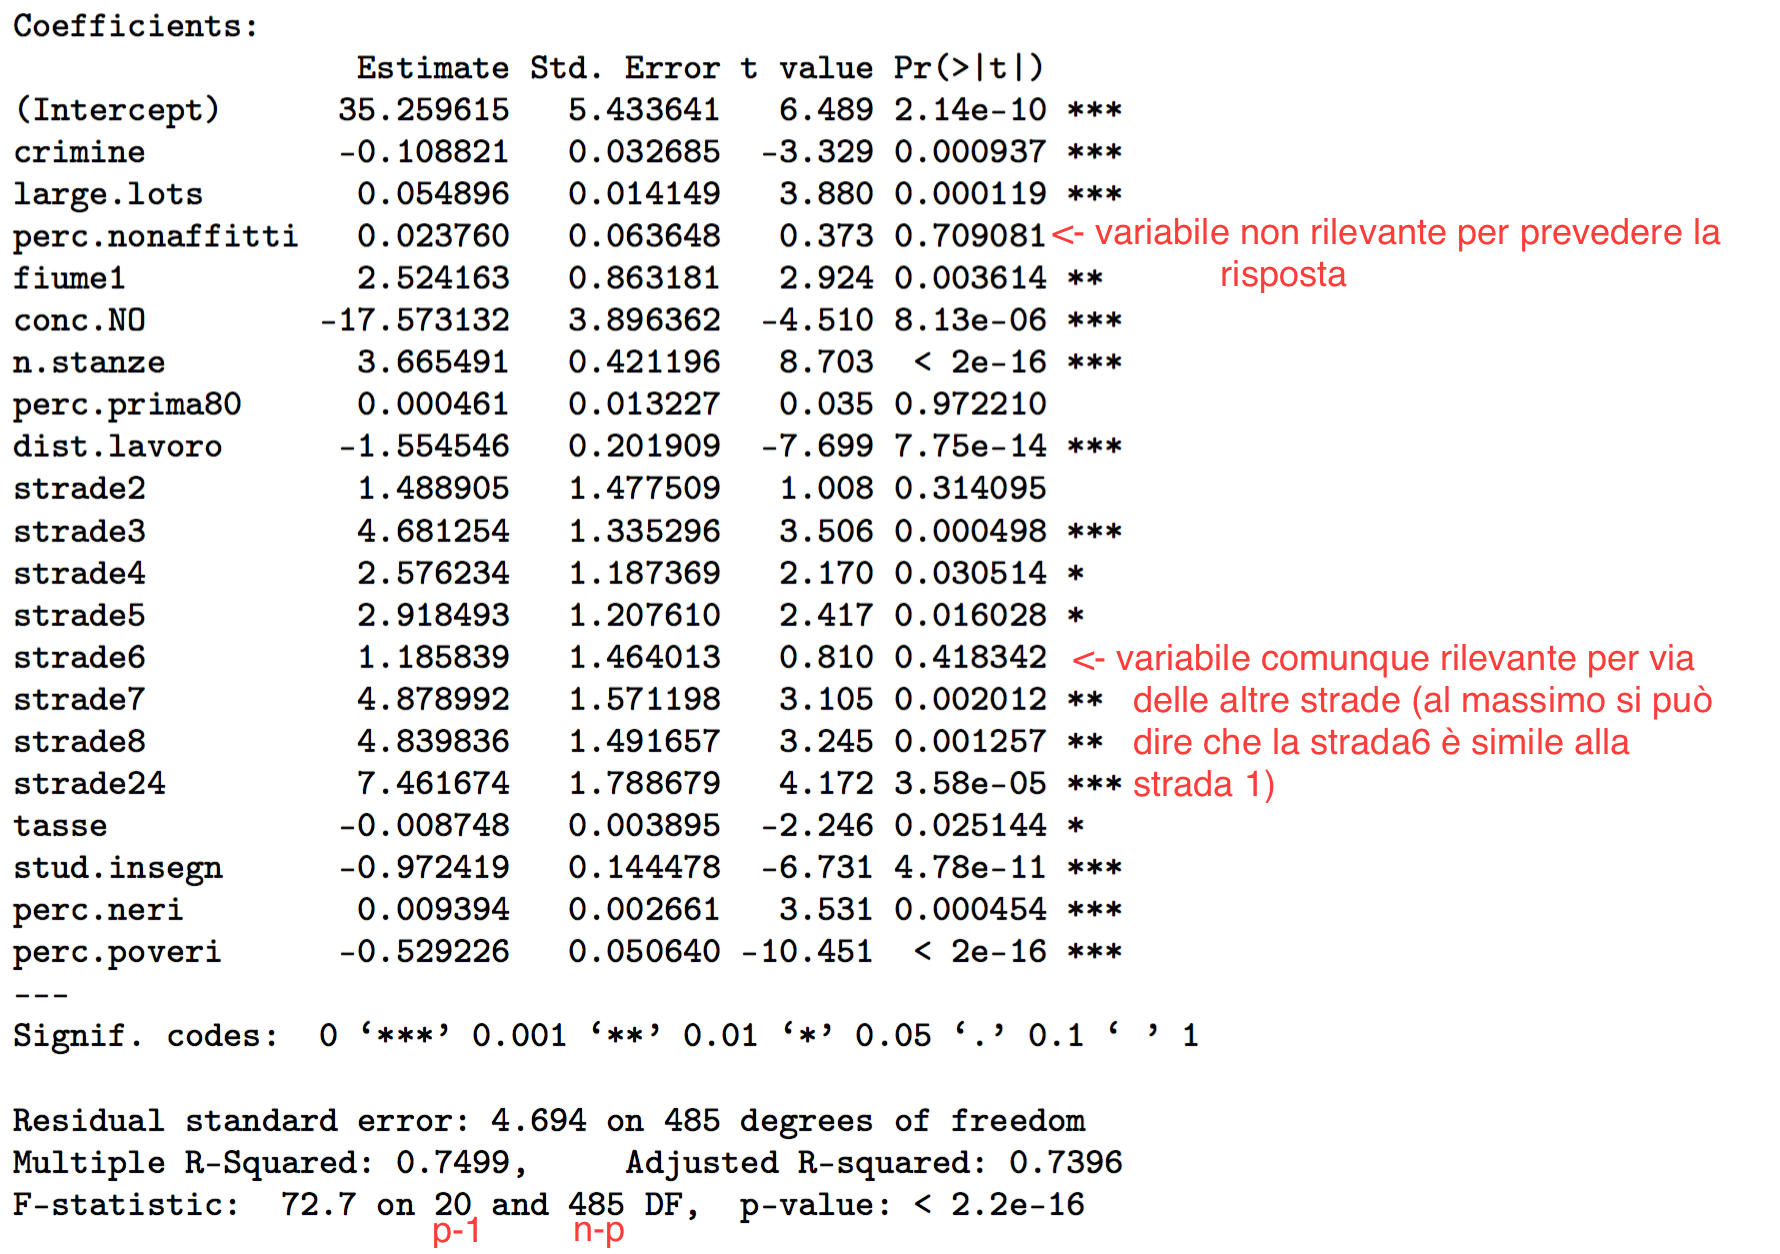
\includegraphics[width=.7\textwidth]{./notes/immagini/l10-fig1.png}
\end{figure}

\subparagraph{Dimostrazione}\label{dimostrazione-1}

Siano $ z_i $ e $ z_{i+p} $ dure caratteri di \textit{Z} a distanza \textit{p}. Siccome $ |\gamma|  \geq p$, i due caratteri possono essere appartenenti solamente o a \textit{X} o a \textit{Y} e mai ad entrambe le stringhe contemporaneamente. 
Pertanto dal momento che sia \textit{X} sia \textit{Y} hanno periodo \textit{p}, i due caratteri devono essere per forza uguali.

Da questo segue il lemma di periodicità che afferma che due periodi distinti \emph{p} e \emph{q} non possono coesistere troppo a lungo in
una stessa stringa senza che la stringa abbia anche periodo \emph{MCD(p,q)}.

\paragraph{Lemma - Lemma di periodicità}\label{lemma---lemma-di-periodicituxe0}

Sia \emph{X} una stringa di lunghezza \emph{n} con due periodi \emph{p}
e \emph{q} non entrambi nulli.

Se $n \geq p + q - MCD(p,q)$ allora la stringa \emph{X} ha anche periodo \emph{MCD(p,q)}.

\begin{figure}[htbp]
\centering
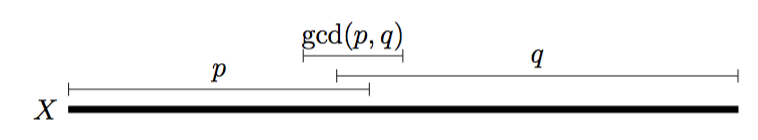
\includegraphics[width=.7\textwidth]{./notes/immagini/l10-fig2.png}
\caption{}
\end{figure}

\subparagraph{Dimostrazione}\label{dimostrazione-2}

Supponendo che $p \leq q$, la dimostrazione viene fatta per induzione su $p+q$.

$(p+q = 1)$ 

Se \emph{p=0} oppure \emph{p=q=0} allora \emph{MCD(p,q) = q} e dunque
\emph{X} ha periodo \emph{MCD(p,q)} perché ha periodo \emph{q}.

$(p+q > 1)$

Se \emph{p=0} o \emph{p=q} vale ancora il caso base.

Se $1 \leq p < q$, si ha che la stringa \emph{X} ha bordi $\alpha$ e $\beta$ di lunghezza \emph{n-p} e \emph{n-q}, questo per il primo lemma dimostrato.

\begin{figure}[htbp]
\centering
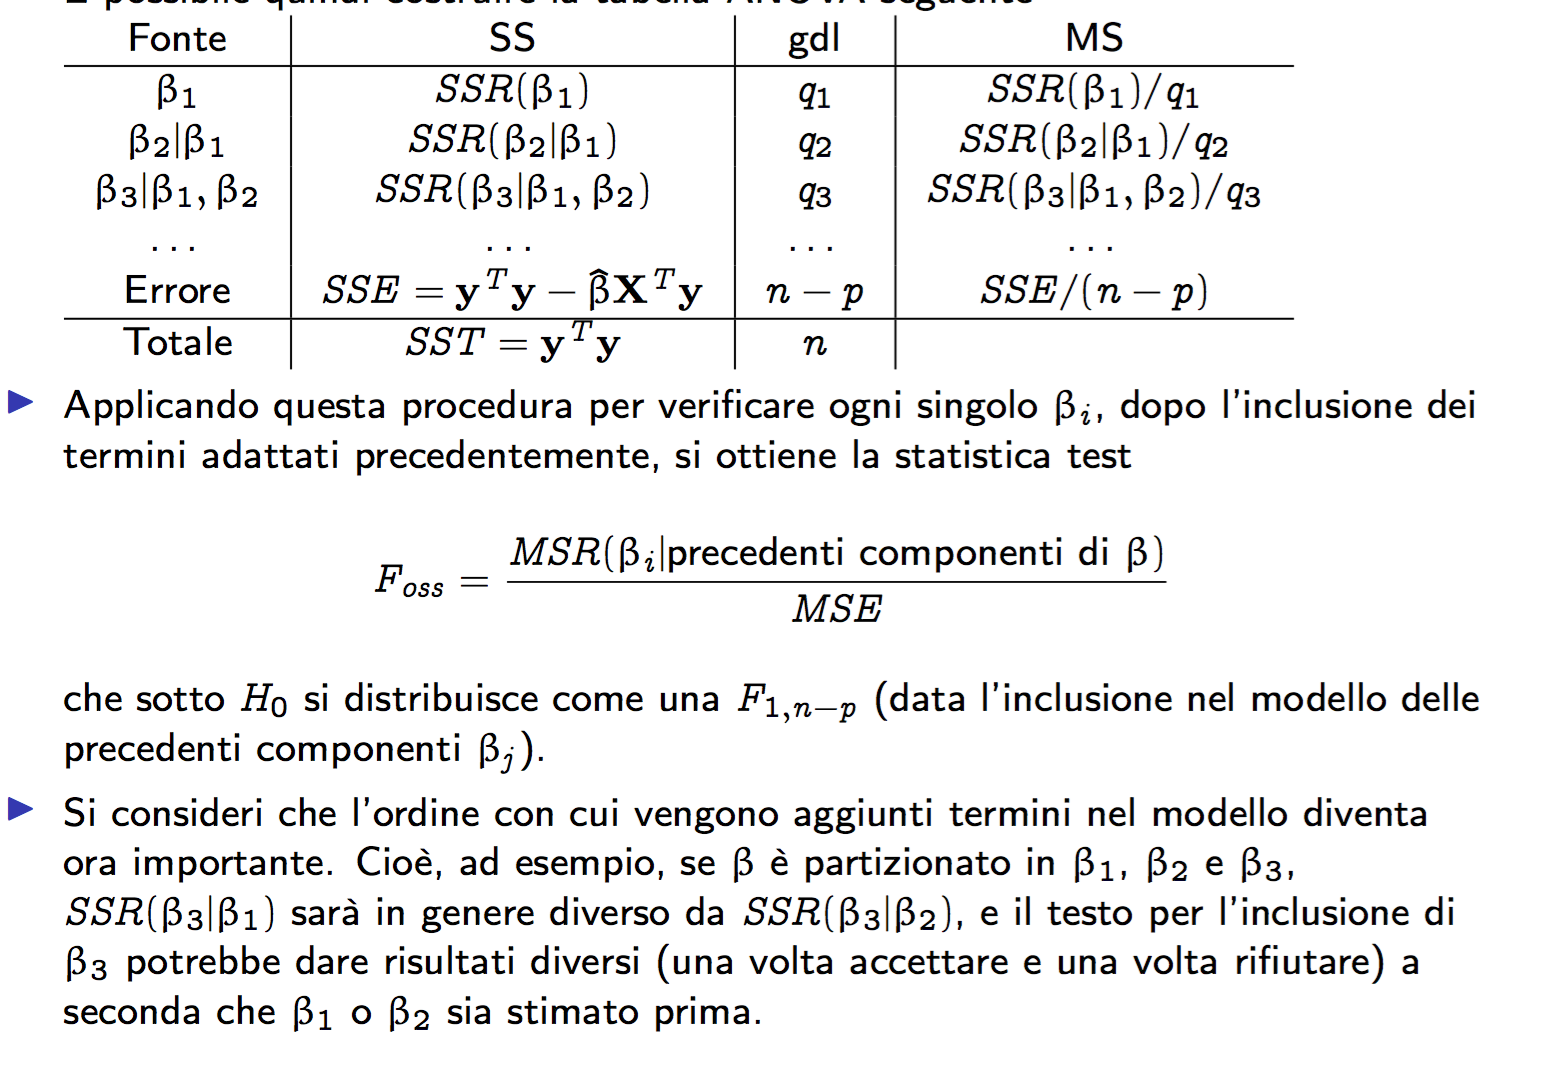
\includegraphics[width=.7\textwidth]{./notes/immagini/l10-fig3.png}
\caption{In verde la stringa $\alpha$ che si ripete con periodo
\emph{p}. In blu la stringa $\beta$ che si ripete con periodo
\emph{q}}
\end{figure}

La stringa $\beta$ essendo bordo di \emph{X} è anche bordo di $\alpha$ dal momento che $\alpha$ è un bordo di \emph{X}, pertanto $\alpha$ ha periodo $r = |\alpha| - |\beta| = q -p$.

Si ha che $p+r < p + q$, quindi è possibile applicare l'ipotesi induttiva, e che \emph{MCD(p,r) = MCD(p,q)}:

\begin{align*}
|\alpha| &\geq p+r-MCD(p,q)\\
 n - p &\geq q - MCD(p,q) 
\end{align*}

$ \alpha $ ha quindi come periodo sia \textit{r} (a causa di $ \beta $), sia \textit{p} (perché è una sottostringa di \textit{X}, la quale ha periodo \textit{p}) e per ipotesi induttiva ha anche periodo $MCD(p,r)$ che per come è definito \textit{r} è uguale a $MCD(p,q)$.

Considerando inoltre che:

\begin{align*}
	2|\alpha| &= (n-p) + (n-p) \\
					 &\geq q - MCD(p,q) + (n-p) \\
					 &\geq n
\end{align*}

perché $ p < q $ per ipotesi e $ MCD(p,q) \leq q - p $ per le proprietà del massimo comun divisore.

Questo implica che il prefisso $ \alpha $ di \textit{X} e il suffisso $ \alpha $ di \textit{X} coprono tutto \textit{X} e pertanto le due stringhe devono sovrapporsi\footnote{Non è possibile applicare il lemma della concatenazione perché non si sa di quanto queste stringhe si sovrappongono.} oppure $ X = \alpha\alpha $.

Presi quindi due caratteri $ x_i $ e $ x_j $ della stringa \textit{X}, tali che $ j - i = MCD(p,q) $ può succedere che i due caratteri appartengano alla stessa $ \alpha $ e quindi siano uguali, perché $ \alpha $ ha periodo $ r = MCD(p,q) $ oppure che $x_i \in \alpha_{(prefisso)} \text{ e } x_j \in \alpha_{(suffisso)} $.

\begin{figure}[htbp]
	\centering
	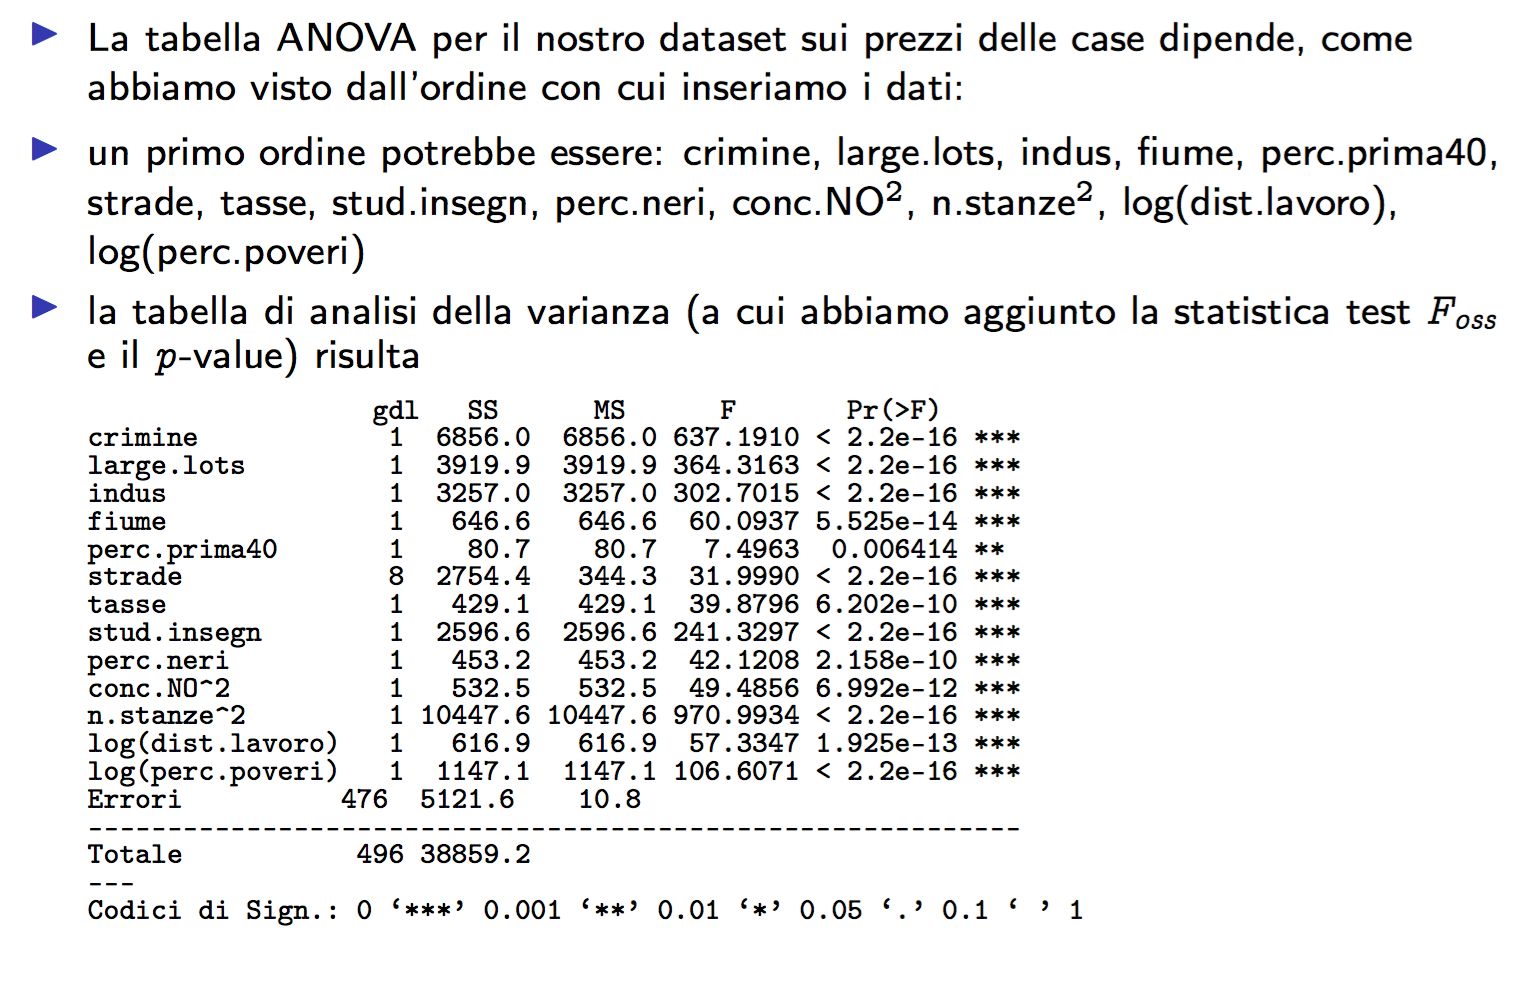
\includegraphics[width=.7\textwidth]{./notes/immagini/l10-fig4.png}
\end{figure}


In questo caso si ha che $ j > n - |\alpha| = p $ e quindi $ j - p \geq 1$. Si può quindi considerare il carattere $ x_{j-p} = x_j$ per via del periodo \textit{p} di $ X $ e che risulta appartenere a $ \alpha_{(prefisso)} $ perché $ p \geq MCD(p,q) $.

La distanza tra $ x_{j-p} \text{ e } x_i$ è $p - MCD(p,q)$, che per definizione è un multiplo di \textit{MCD(p,q)}, pertanto si ha che $ x_{j-p} \text{ e } x_i$ appartengono ad $ \alpha_{(prefisso)} $ che ha periodo \textit{MCD(p,q)}, pertanto $ x_{j-p} = x_i = x_j $ e di conseguenza \textit{X} ha periodo \textit{MCD(p,q)}.


	\textbf{Sottostringa}: serie di caratteri vicini

\textbf{Sottosequenza}: serie di caratteri non necessariamente vicini.

\section{Pattern matching di base}\label{pattern-matching-di-base}

Effettua il pattern matching esatto, cercando la sotto stringa \emph{P}
dentro la stringa \emph{T}.

\begin{breakablealgorithm}
	\caption{Ingenuo: Pattern matching ingenuo}
	\begin{algorithmic}[1]
	\Function{Ingenuo}{$ (P,T) $}
	\State $  $ \Comment{\textit{T} ha lunghezza \textit{n} e \textit{P} ha lunghezza $ m \leq n $}
	\For{$ i = 1 \: \text{to} n-m+1 $}
		\State $ j \gets 1 $
		\While{$ j \leq m \:\text{and} \:P[j] = T[i+j-1] $}
	        \State $ j \gets j + 1 $
	    \EndWhile
	    \If{$ j > m $}
	        \State Segnala l'occorrenza del pattern
	    \EndIf
	\EndFor
	\EndFunction
\end{algorithmic}
\end{breakablealgorithm}

\subsection{Utilizzo della sentinella}\label{utilizzo-della-sentinella}

La prima modifica che si può fare all'algoritmo per migliorarne
l'efficienza è quello di ridurre il test del \texttt{while}, rimuovendo
il controllo sulla lunghezza del pattern, riducendo così le operazioni
da 3 a 2.

Questo viene fatto aggiungendo una sentinella alla fine del pattern,
ovvero viene aggiunto al pattern un carattere che non compare
nell'alfabeto della stringa.

Perché questo funzioni è necessario aggiungere un carattere diverso
dalla sentinella anche alla fine di \emph{T} per permettere il match del
pattern anche quando questo è un suffisso della stringa.

\begin{breakablealgorithm}
	\caption{Ingenuo: Pattern matching ingenuo}
	\begin{algorithmic}[1]
		\Function{Ingenuo-2}{$ (P,T) $}
        \State //\textit{T} ha lunghezza \textit{n} e \textit{P} ha lunghezza $ m \leq n $
        \State $ P[m+1] \gets \$ $
        \State $ T[n+1] \gets @$
        \For{$ i = 1 \: \text{to } n-m+1 $}
	        \State $ j \gets 1 $
	        \While{$ P[j] = T[i+j-1] $}
		        \State $ j \gets j + 1 $
	        \EndWhile
	        \If{$ j > m $}
		        \State Segnala l'occorrenza del pattern
	        \EndIf
        \EndFor
        \EndFunction
\end{algorithmic}
\end{breakablealgorithm}

Nel caso non sia possibile modificare il testo si può togliere il
\texttt{+1} del ciclo \texttt{for} e sostituirlo con un \texttt{if} che
verifica l'uguaglianza dell'ultimo carattere.

D'ora in avanti assumeremo la presenza dei due caratteri sentinella.

\subsection{Riduzione del numero di confronti}\label{riduzione-del-numero-di-confronti}

Se il pattern contiene delle sottostringhe uguali, è possibile ridurre
il numero di controlli.

Ad esempio nel caso sotto riportato, l'algoritmo \textsc{Ingenuo}
effettua 20 confronti.

\begin{figure}[htbp]
\centering
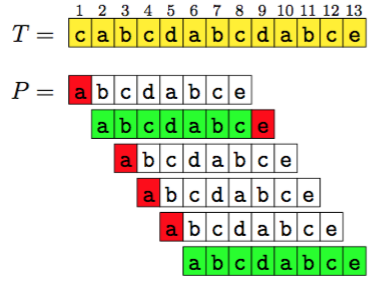
\includegraphics[width = .4\textwidth]{./notes/immagini/l11-fig1.png}
\end{figure}

Ovvero è possibile evitare il confronto tra l'inizio del pattern e il
terzo carattere del testo, perché si sa già che il terzo carattere del
testo è uguale al secondo carattere del pattern, il quale è diverso dal
primo carattere del pattern. Lo stesso ragionamento vale anche per i due
confronti successivi.

Ma si può fare di più, perché il pattern ha una sottostringa uguale al
suo prefisso, ovvero i caratteri 7-8-9 della del testo sono uguali ad
una sottostringa del pattern che coincide con il prefisso del pattern e
dal momento che questo è già questa uguaglianza è già stata verificata,
si possono ridurre ulteriormente i confronti.

\begin{figure}[htbp]
\centering
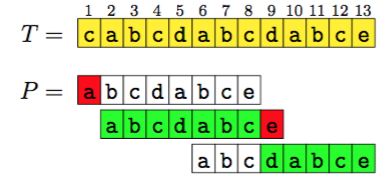
\includegraphics[width = .4\textwidth]{./notes/immagini/l11-fig2.png}
\end{figure}

Per poter applicare queste osservazioni ad un algoritmo è necessario
effettuare delle pre-elaborazioni delle stringhe.

\subsection{Pre-elaborazione fondamentale}\label{pre-elaborazione-fondamentale}

Data una stringa \emph{S} di lunghezza \emph{n}, la funzione
$\pi_i^S$ calcola la lunghezza del prefisso di \emph{S} più lungo
che occorre nella posizione \emph{i} di \emph{S}.

Quindi $\pi_i^S$ è il massimo \emph{h} tale che

$$
S[1,h] = S[i, i+h-1]
$$

Ad esempio:

\begin{figure}[htbp]
\centering
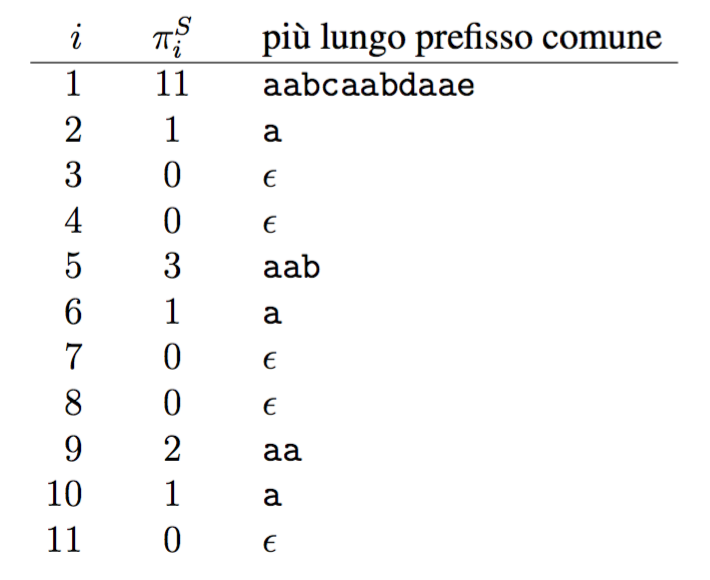
\includegraphics[width = .4\textwidth]{./notes/immagini/l11-fig3-bis.png}
\caption{$\pi_i$ per \textit{S=}\texttt{aabcaabdaae}.}
\end{figure}

Da notare che $Y = S[i, i+\pi_i -1]$ per definizione è un occorrenza in \textit{S} della stringa $S[1, \pi_i -1]$, pertanto si ha che \textit{Y} è un bordo della stringa $S[1, i +\pi_i -1]$. 
Per la relazione tra prefisso e bordo si ha quindi che $S[1, i +\pi_i -1]$ ha periodo $p = i -1$.

Si ha inoltre che la stringa $S[1, i +\pi_i -1]$ è il più lungo prefisso di \textit{S} con periodo $p= i-1$.

Questo perché se $i = 1$, si ha che il prefisso \textit{Y} coincide con \textit{S} e $p=0$, ottenendo periodo e bordo degeneri.

Se invece $ i \geq 2 $ si ha che, se $i + \pi_i -1 = n $, \textit{Y} è anche un suffisso di \textit{S}, pertanto non possono esserci altri prefissi con periodo $p = i -1$ più lunghi perché è la stringa \textit{S} è terminata.
Oppure se $i + \pi_i -1 \neq n $ vuol dire che il carattere $ S[\pi_i + 1] $ è diverso dal carattere $ S[i+\pi_i] $ per definizione di $ \pi_i $ e quindi non può esistere un prefisso $ S[1, \pi_i +1] $ con periodo $p = i -1$ perché $ S[\pi_i  + 1 + p] = S[\pi_i + i] $ che per ipotesi è diverso da $ S[\pi_i +1] $.

Le varie sottostringhe $ S[i, i + \pi_i -1 ] $ non sono necessariamente disgiunte ma possono sovrapporsi.

\subsubsection{Estremi massimi}

Fissato un $ i \geq 2 $, si ottengono varie stringhe $ S[j, j + \pi_j -1] $ con $ 2 \leq j \leq i $.

Tra tutte queste stringhe è possibile identificare la stringa che ha come valore dell' \textbf{estremo destro massimo}:

$$
r_i = \max \{ j + \pi_j -1 | \: 2 \leq j \leq i\}
$$

L'estremo sinistro associato viene indicato con 

$$
l_i = \arg\max\limits_{j} \{ j + \pi_j -1 | \: 2 \leq j \leq i\}
$$

Nel caso ci siano più sottostringhe con lo stesso estremo destro, viene scelto come estremo sinistro uno a caso tra quelli possibili.

La stringa $ S[l_i, r_i] $ risulta quindi essere la sottostringa di \textit{S} più lunga che è anche un prefisso e che inizia prima dell'indice \textit{i}.

\begin{figure}[htbp]
	\centering
	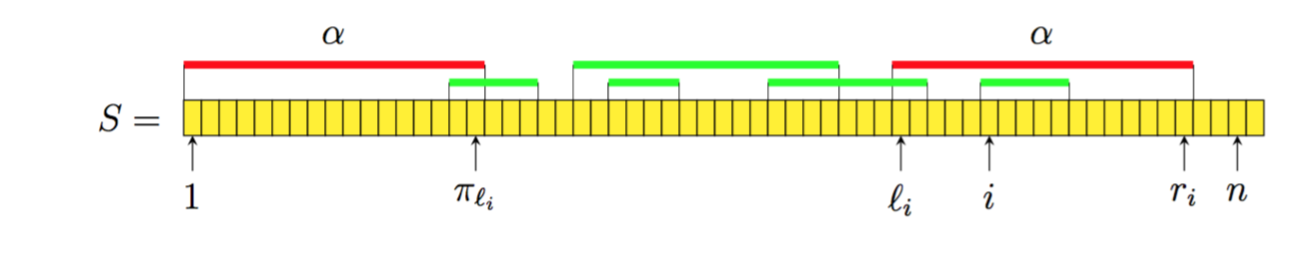
\includegraphics[width = .9\textwidth]{./notes/immagini/l11-fig4-bis.png}
	\caption{Alcune occorrenze di prefissi di \textit{S} che iniziano tra le posizioni \textit{2} e \textit{i}. L'occorrenza che termina più a destra è evidenziata in rosso.}
\end{figure}

Si ha quindi che $ S[1,r_i] $ è il più lungo prefisso di \textit{S} con periodo $ 1 \leq p < i $ e che la stringa $ S[l_i, r_i] $ è la sottostringa di \textit{S} che termina più a destra tra tutte quelle che sono uguali ad un prefisso di \textit{S}.

Ad esempio se 

$$
S = \text{\texttt{aabaabcadaabaabce}}
$$

il massimo destro con $ 2 \leq j \leq 15 $ è $ r_{15} = 10 + \pi_{10} -1 = 16$, perché $ \pi_{10} = 7$, e $ l_{15} = 10 $ che è la posizione in cui inizia la sottostringa \texttt{aabaabc}.

\subsection{Pre-elaborazione fondamentale in tempo lineare}\label{preambolazione-fondamentale-in-tempo-lineare}

Seguendo l'approccio di definizione il tempo richiesto è
$O(n^2)$, ma è possibile scendere a $O(n)$.

Supponiamo che \emph{S} termini con un carattere diverso da tutti gli
altri che compaiono nella stringa. Questo non è un problema perché si
può sempre aggiungere una sentinella.

L'algoritmo calcola $\pi_1 = n$ e poi calcola i valori $\pi_i, r_i, l_i$ per $i = 2,\ldots, n$, basandosi su un'array $ pref[1\ldots n] $ il quale conterrà i vari $ \pi_i $ e due variabili, \textit{r} e \textit{l}, le quali andranno a memorizzare gli estremi massimi tra gli indici precedente calcolati.

Come prima cosa viene effettuato il calcolo di $ \pi_2 $ confrontando da sinistra a destra i caratteri di $S[2,n]$, cosi facendo si ha che $ r = \pi_2 +1 $ e $l = 2$.

Assumendo induttivamente di aver calcolato $ \pi_j $ per ogni $ j = 2, \ldots, i-1$, si ha che $ r = r_{i-1} = \pi_{i-1} +1 $ e $ l = l_{i-1} $.

Durante il calcolo di $ \pi_i $ possono verificarsi 2 casi:

\begin{enumerate}
	\item $ i > r $: non si hanno informazioni riguardo ai caratteri che seguono \textit{i}, quindi viene effettuato il calcolo di $ \pi_i $ normalmente, andando ad effettuare i confronti da sinistra a destra tra $ S[i,n] $ e \textit{S}. Il valore di $ \pi_i $ è allora uguale alla lunghezza \textit{h} del massimo prefisso comune e $ r = i  + \pi_i +1 $ e $ l= i $.
	\item $ i \leq r$: il carattere \textit{S[i]} è contenuto nella sottostringa $ \alpha = S[l,r] $ la quale è anche prefisso di \textit{S}. Si ha quindi che il carattere \textit{S[i]} compare anche nella posizione $ i' = i - l +1 $ di \textit{S} e per lo stesso motivo la stringa $ \beta = S[i,r] $ compare anche in $ S[i', \pi_l] $.
	\begin{figure}[htbp]
		\centering
		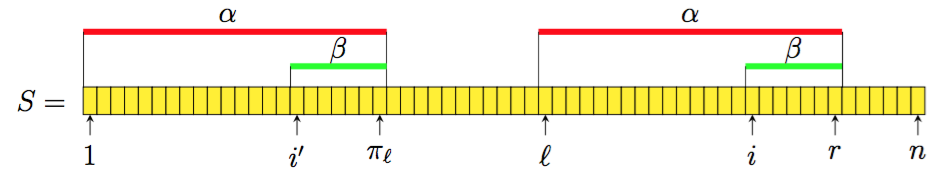
\includegraphics[width = .8\textwidth]{./notes/immagini/l11-fig3.png}
	\end{figure}
	In \textit{i'} occorrerà un prefisso $ \gamma $ di \textit{S} di lunghezza $ \pi_{i'} $, che può anche essere degenere.
	Questo prefisso occorrerà a partire dalle posizioni \textit{1} e \textit{i'} e potrà essere contenuto o contenere la sottostringa $ \beta $.
	Ne segue che \textit{S} e \textit{S[i,n]} hanno un prefisso in comune di lunghezza uguale al minimo tra $ \pi_{i'} $ e $ |\beta| = r - i +1 $.
	\begin{enumerate}
		\item $ \pi_{i'} < |\beta| $: il prefisso che inizia in \textit{i} ha la stessa lunghezza di quello che inizia in \textit{i'}, ed avendo già calcolato la lunghezza di quel prefisso si ha che $ \pi_i = \pi_{i'} $ senza effettuare alcun confronto.
		\begin{figure}[htbp]
			\centering
			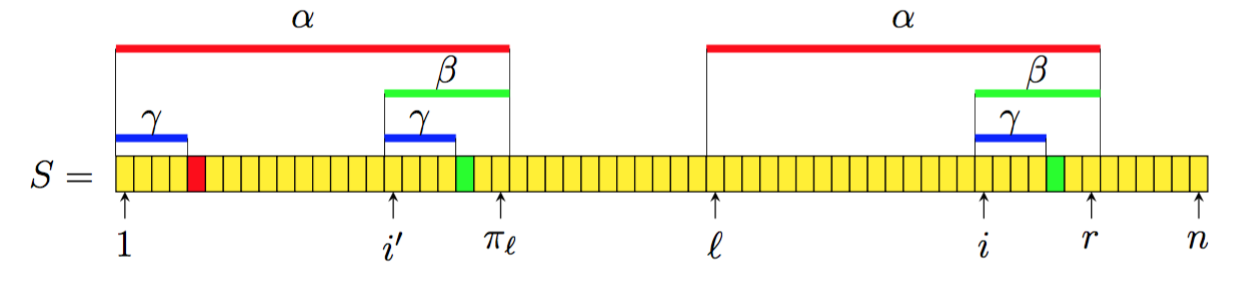
\includegraphics[width = .8\textwidth]{./notes/immagini/l11-fig5.png}
		\end{figure}
		\item $ \pi_{i'} \geq |\beta|$: l'intera sottostringa $ \beta = S[i,r] $ deve essere un prefisso di \textit{S} e quindi $\pi_i \geq |\beta| = r - i +1$. L'algoritmo calcola quindi la lunghezza \textit{h} del massimo prefisso comune tra \textit{S} e \textit{S[i,n]} a partire dai caratteri $ |\beta| + 1 $ e $ i + |\beta| $, fino a che non trova un mismatch. A questo punto vengono posti $ \pi_i =h,\: r= i + \pi_i -i \: \text{e} \: l = i $.
	\end{enumerate}
	
\end{enumerate}

\begin{breakablealgorithm}
	\caption{Prefisso: Preelaborazione del prefisso in tempo lineare}
	\begin{algorithmic}[1]
		\Function{Prefisso}{$ S $}
		    \State // S stringa di lunghezza n > 1 con sentinella alla fine
		    \State $ pref[1] \gets n $  \Comment{$ \pi_i, \pi_1 = n$}
		    \State $ h \gets 0 $
		    \While{$ S[1+h] = S[2+h] $}\Comment{Calcola $\pi_2$}
		        \State $ h = h +1 $
		    \EndWhile
		    \State $ pref[2] \gets h $
		    \State  $ l \gets 2 $
		    \State $ r \gets 2 + h - 1$
		    \For{$ i = 3 \: \text{to} \: n $}
			    \If{$ r < i $} \Comment{Caso 1}
			        \State $ h \gets 0$
		            \While{$ S[1+h] = S[i+h]$}
		                \State $ h \gets h + 1 $
		            \EndWhile
		            \State $ pref[i] \gets h$
		            \State $ l \gets i $
		            \State $ r \gets i + h -1 $
		        \Else \Comment{Caso 2}
				    \If{$pref[i-l+1] < r - i +1$} \Comment{Caso 2a}
		                \State $pref[i] \gets pref[i - l +1]$
		            \Else \Comment{Caso 2b}
		               \State $h \gets r - i +1$
		                \While{$S[1+h] = S[i +h]$}
		                    \State $ h \gets h +1 $
		                \EndWhile
		                \State $pref[i] \gets h$
		                \State $l \gets i$
		                \State $ r \gets i +h -i$
			         \EndIf
		          \EndIf
		    \EndFor
		    \State \Return $ pref $
		   \EndFunction
	\end{algorithmic}
\end{breakablealgorithm}

La correttezza dell'algoritmo deriva da quanto detto prima

\paragraph{Complessità}\label{complessituxe0}

Se non viene presa in considerazione la complessità dei cicli
\texttt{while} si ha che la complessità è data da \emph{O(n)}.

I cicli \texttt{while} terminano quando viene trovato un mismatch e al
massimo vengono trovati \emph{n-1} mismatch (1 dal \texttt{while}
esterno, $n-2$ dai \texttt{while} dentro il ciclo \texttt{for}).

Ad ogni confronto con successo, il carattere destro ($S[i+h]$)
viene spostato a destra di 1 e, una volta terminato il \texttt{while}, questo viene posto a $r = i + h - 1$, ovvero risulta essere il carattere alla posizione $S[r+1]$.

All'iterazione successiva il ciclo \texttt{while} inizia con carattere destro $S[i]$ se $i > r$\footnote{Viene quindi sposto a destra perché $ i \geq r+1 $} altrimenti inizia con $S[i + h]$ con $h = r - i + 1$. In entrambi i casi il carattere destro non si sposta mai a sinistra durante l'esecuzione dell'algoritmo. 
Pertanto vengono eseguiti al più $n-1$ confronti con successo. +
Si ottiene quindi una complessità per i \texttt{while} di $O(2n-2)$.

La complessità totale dell'algoritmo è data da $O(n) +\textit{ Complessità while }= O(n) + O(2n-2) = O(n)$.

\subsubsection{Matching esatto in tempo lineare}\label{matching-esatto-in-tempo-lineare}

Per effettuare il pattern matching in tempo $O(m+n)$ del pattern \emph{P} in \emph{T} è possibile utilizzare una versione leggermente modifica della funzione prefisso sulla stringa \emph{S = P\$T}, dove \$ è un simbolo che non è presente nelle due stringhe.

Questo viene fatto calcolando $ \pi_i^S $ per $ i = 2, \ldots n + m +1 $.
Siccome \$ non compare in nessuna delle due stringhe, si ha che $ \pi_i \leq m \: \forall \: i $ perché per ipotesi la sottostringa \textit{P\$} non può comparire all'interno di \textit{T}.
Inoltre, $ \forall \: i \geq m +1 : \pi_i = m $ si ha che $i - m - 1$ identifica l'inizio di un'occorrenza di \textit{P} in \textit{T}, perché $ \pi_i = m $ indica la presenza di prefisso di lunghezza \textit{m} a partire dalla posizione \textit{i}, ma la sottostringa prefissa di lunghezza \textit{m} coincide per costruzione con \textit{P}, quindi \textit{i} indica l'inizio di un'occorrenza del pattern \textit{P} nella stringa \textit{P\$T}.

Dal momento che il prefisso viene calcolato in tempo lineare rispetto la lunghezza della stringa, si ottiene una funzione di pattern matching con complessità lineare.

Altre caratteristiche di questo algoritmo sono:
\begin{itemize}
	\item il \textbf{consumo lineare di memoria} rispetto la lunghezza del pattern $ O(m) $, perché è possibile evitare di tenere in memoria tutti $ \pi_i $ con $ i >m $ perché tutti i valori \textit{i'} del caso 2 faranno sempre riferimento ai $ \pi_i \: \text{con}\: i \leq m $
	\item che non è necessario conoscere tutto l'alfabeto, basta avere la possibilità di confrontare i caratteri.
\end{itemize}

\subsubsection{Esercizio - Identificare una rotazione}

Date due stringhe \textit{X} ed \textit{Y} di uguale lunghezza \textit{n}, determinare in tempo lineare \textit{O(n)}, se \textit{Y} è una rotazione circolare di \textit{X}.
Ovvero se è possibile identificare due stringhe $ \alpha $ e $ \beta $ tali che $ X = \alpha\beta $ e $ Y = \beta\alpha $.

\paragraph{Soluzione}

Si concatenano le stringhe in modo da formare $ S = Y\$XX $, se eseguendo la preelaborazione trovo un prefisso di lunghezza \textit{n} a partire dal $n+1$ vuol dire che \textit{Y} compare tra le due \textit{X} e quindi le due stringhe sono la rotazione di una stessa stringa.

\subsubsection{Esercizio - Massima sottostringa comune}

Date due stringhe \textit{X} e \textit{Y} di lunghezza \textit{m} e \textit{n} calcolare, in tempo lineare, il più lungo suffisso di \textit{X} che è anche prefisso di \textit{Y}. 
Ovvero la sottostringa $ \gamma $ di lunghezza massima tale che $ X = \alpha\gamma \: \text{e} \: Y = \gamma\alpha$.

\paragraph{Soluzione}

L'idea è quella di concatenare due stringhe in modo da formare $ S= Y\$X $, dove \$ è un carattere che non compare in nessuna delle due stringhe, per poi effettuare la preelaborazione.

Se $ \pi_2^S = 0$ non c'è nessuna sottostringa uguale al prefisso di \textit{Y}, quindi $ \gamma = \epsilon $, altrimenti se  $ 0 < \pi_2^S = k \leq m$ si ha che c'è un'occorrenza all'interno di \textit{S} del prefisso di \textit{Y} lunga \textit{k}, ma non si ha alcuna garanzia che questa sia un suffisso per \textit{X}.

Se  $ \pi_{n+m+1-k}^S = k$ si ha che a partire dal carattere $ n+m+1-k $ c'è un match di una sottostringa di lunghezza \textit{k} che per costruzione è anche suffisso di \textit{X}, pertanto $ \gamma = Y[1,k] $, altrimenti la sottostringa precedentemente identifica si trova o all'interno di \textit{Y} o all'interno di \textit{X}, pertanto $ \gamma = \epsilon $.

\todo[inline]{Quasi corretto, bisogna andare a vedere i $ \pi_j $ per trovare il suffisso più lungo che è anche prefisso.}



	\subsection{Verifica delle false occorrenze}\label{verifica-delle-false-occorrenze}

Il metodo di Rabin-Karp può trovare delle false occorrenze anche se la probabilità che queste compaiano è molto bassa .

L'algoritmo di Mathukrishnan serve per verificare se ci sono o meno delle false occorrenze in tempo \emph{O(n)}.

L'algoritmo prende in input la lista delle posizioni in cui c'è un'occorrenza vera o meno e identifica una falsa occorrenza utilizzando la distanza tra queste due posizioni.

Siano $ pos_{i-1} $ e $ pos_{i} $ due occorrenze consecutive segnalate dall'algoritmo di Karp e sia $ d = pos_{i} - pos_{i-1}$ la distanza tra queste.

Se $ d \leq m/2 $\footnote{Perché una stringa sia periodica, questa deve avere un periodo $ 0 \leq 2d \leq m $.} ed entrambe sono occorrenze effettive, il pattern \textit{P} ha un bordo di lunghezza $ m -d $ e quindi $ d  $ è un periodo sia del pattern, che della stringa $ T[pos_{i-1}, pos_{i} +m -1] $.

Inoltre, se \textit{P} avesse anche un periodo proprio $ p < d $ la porzione di testo $ T[pos_{i-1}, pos_{i} +m -1] $ dovrebbe avere anche essa il periodo $ p $ e quindi dovrebbe esserci un'occorrenza del pattern anche a partire da $ pos_{i-1} + p$, ma siccome non c'è questa occorrenza, la stringa non può avere periodo $ p $, quindi $ d $ è il più piccolo periodo proprio di $ P $.

L'algoritmo suddivide quindi le possibili occorrenze in \textbf{corse}, ovvero una sequenza di possibili occorrenze tali che $ pos_{i} - pos_{i-1} \leq m/2  $.

Se la corsa è composta da una sola posizione, l'algoritmo verifica direttamente se c'è un'occorrenza del pattern, confrontando il pattern con la stringa.

Se invece la cosa contiene più elementi $ pos_s, pos_{s+1}, \ldots, pos_{t} $, l'algoritmo verifica direttamente le prime due occorrenze $pos_{s}$ e $ pos_{s+1} $, se c'è una falsa occorrenza l'algoritmo termina, altrimenti la distanza $ d = pos_{s} - pos_{s+1} $ è il più piccolo periodo del pattern \textit{P} e quindi se per qualche $ i = s+2, \ldots, t  $ si ha che $ pos_i - pos_{i-1} \neq d $, l'algoritmo termina segnalando una falsa occorrenza.

Questo è corretto perché se $ pos_i - pos_{i-1} < d $, $ d $ non sarebbe il periodo minimo mentre se $ pos_i - pos_{i-1} > d $, c'è una falsa occorrenza perché dovrebbe esserci anche un'occorrenza intermedia.

Se l'algoritmo trova che tutte le distanze sono uguali a $ d $ deve soltanto controllare che la parte $ T[pos_s +m, pos_t + m -1] $ abbia effettivamente periodo $ d $ e questo viene fatto in tempo proporzionale alla lunghezza, confrontando tra loro i caratteri.


\begin{breakablealgorithm}
\caption{\textsc{MathukrishnanTest}: verifica della presenza di false occorrenze}
\begin{algorithmic}[1]
\Function{MathukrishnanTest}{$P,T,pos,k$}
	\If{$ k = 0 $}
		\State \Return false
	\EndIf
	\State $ j \gets 1 $
	\While{$ P[j] = T[pos[1] + j -1] $}
		\State $ j \gets j+1 $
	\EndWhile
	\If{$ j \leq m $} \Comment{è una falsa occorrenza}
		\State \Return True
	\EndIf
	\State $ i \gets 2 $
	\While{$ i \leq k $}
		\State $ j \gets 1 $
		\While{$ P[j] = T[pos[i] + j -1] $}
			\State $ j \gets j+1 $
		\EndWhile
		\If{$ j \leq m $} \Comment{è una falsa occorrenza}
			\State \Return True
		\EndIf
		\If{$ pos[i] - pos[i-1] \leq m/2$}
			\State $ s \gets i -1 $
			\State $ p \gets pos[s+1] - pos[s] $
			\While{$ i+1 \leq k \textbf{ and  } pos[i+1] - pos[i] = p$}
				\State $ i \gets i+1 $
			\EndWhile
			\If{$ i+1 \leq k \textbf{ and  } pos[i+1] - pos[i] \neq p$}
				\State \Return True
			\EndIf
		\EndIf
		\For{$ j \gets pos[s] +m +p \textbf{ to } pos[i] +m -1 $}\Comment{tutte le posizioni della corsa sono a distanza corretta, controllo se la porzione di testo ha periodo $p $}
			\If{$ T[j] \neq T[j-p] $}
				\State \Return True
			\EndIf
		\EndFor
	\EndWhile
\EndFunction
\end{algorithmic}
\end{breakablealgorithm}

\subsubsection{Complessità}\label{complessituxe0}

Per ogni corsa si hanno al massimo $pos_t - pos_s - d$ caratteri da verificare, se il risultato è negativo viene segnalata una falsa occorrenza e l'algoritmo termina, altrimenti passa alla corsa successiva.

Durante la verifica di una corsa, ogni carattere del testo viene confrontato al massimo 2 volte con i caratteri del pattern più 1 volta con il carattere successivo del testo.

Dal momento che le corse distinte non si sovrappongono, si ha che vengono fatti al massimo \emph{O(3n)} confronti, che portano ad una complessità di \emph{O(n)}.

\section{Alberi dei suffissi}\label{alberi-dei-suffissi}

L'albero dei suffissi permette di evidenziare maggiormente la struttura interna di una stringa, permettendo così di risolvere in tempo lineare il pattern matching esatto, così come altri problemi di pattern matching più complesso.

Con il pattern matching esatto è possibile effettuare una pre-elaborazione del testo in \emph{O(n)} dopo la quale è possibile verificare in tempo \emph{O(m)} la presenza del pattern, rendendo questi algoritmi adatti ai problemi che hanno un testo fisso che deve essere matchato con più pattern distinti.

L'\textbf{albero dei suffissi} per una stringa \emph{S} di lunghezza \emph{n} è costituito da:

\begin{itemize}
\item  \emph{n} foglie numerate da 1 ad \emph{n}.
\item  Ogni nodo interno, eventualmente esclusa la radice, ha almeno due figli.
\item  Ogni arco è etichettato con una sottostringa di \emph{S}.
\item  Due archi uscenti dallo stesso nodo non possono avere etichette che iniziano con lo stesso carattere.
\item  La concatenazione delle etichette lungo il cammino dalla radice alla foglia etichettata \emph{i} è il suffisso $S[i,n]$ di lunghezza $ n-i+1 $
\end{itemize}

\begin{figure}[htbp]
\centering
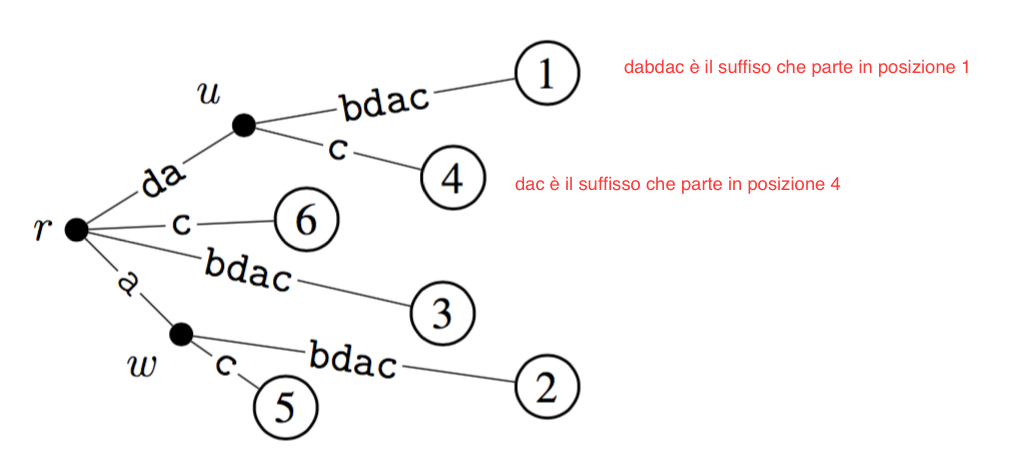
\includegraphics[width=.7\textwidth]{./notes/immagini/l19-fig1.png}
\caption{Albero dei suffissi della stringa $ S = dabdac $}
\end{figure}

Da notare che non sempre è possibile costruire l'albero dei suffusi, perché se un suffisso è anche prefisso di un altro suffisso, il cammino relativo a quel suffisso termina in un nodo interno dell'albero, violandone la definizione. 
Per evitare questo problema è necessario aggiungere un carattere sentinella alla fine della stringa. Assumeremo che questa ci sia sempre.

Nell'esempio \emph{S=dabdac} è \emph{c} che fa da sentinella, se non ci fosse non sarebbe possibile costruire l'albero.

L'\textbf{etichetta di un cammino} è la concatenazione delle etichette degli archi del cammino, mentre l'etichetta di un nodo \emph{u} è data dall'etichetta del cammino dalla radice al nodo.

Se l'etichetta di un arco $ (u,v) $ tra due nodi interni ha lunghezza \textit{k} maggiore di 1, l'arco è in realtà diviso in \textit{k} parti, una per ogni carattere dell'etichetta, mediante $ k-1 $ \textbf{nodi impliciti} le cui etichette sono la concatenazione dell'etichetta di \textit{u} con i caratteri dell'etichetta dell'arco $ (u,v) $ che precedono il nodo stesso.

\subsection{Matching esatto con l'albero dei suffissi}\label{matching-esatto-con-lalbero-dei-suffissi}

\begin{enumerate}
	\item Costruisci l'albero dei suffissi \textit{A} per il testo \textit{T}.
	\item Confronta i caratteri del pattern \textit{P} con i caratteri dell'unico cammino in \textit{A} individuato da essi. Questo cammino è unico perché tutti gli archi uscenti di un nodo sono associati a caratteri distinti. Seguendo questo cammino si possono verificare due casi:
	\begin{enumerate}
		\item Si esauriscono i caratteri del pattern e si passa al passo successivo
		\item Ci sono ancora dei caratteri del pattern ma non è possibile proseguire il cammino, in questo caso non ci sono occorrenze del pattern nel testo e l'algoritmo può terminare.
	\end{enumerate}
	\item Se si arriva alla fine del pattern, allora questo è uguale all'etichetta del nodo \textit{u} a cui si è arrivati, indipendentemente dal fatto che \textit{u} sia un nodo implicito o meno. Il pattern \textit{P} è quindi prefisso di tutti i suffissi associati alle foglie del sotto-albero radicato in \textit{u}. Le posizioni d'inizio di questi suffissi sono quindi tutte e sole le posizioni in cui \textit{P} occorre in \textit{T} e dal momento che queste posizioni sono memorizzate nelle foglie del sotto-albero, è sufficiente esplorarlo fino alle foglie per risalire alle posizioni di occorrenza del pattern.
\end{enumerate}

\subsubsection{Complessità del matching esatto}\label{complessituxe0-del-matching-esatto}

C'è una complessità \emph{O(n)} per la costruzione dell'albero (che per il momento non è stata vista).

Durante il secondo passo, per ogni carattere del pattern viene fatto
\begin{itemize}
	\item Un confronto se l'algoritmo sta analizzando un nodo implicito (c'è un solo arco uscente)
	\item Al più tanti confronti quanti sono i caratteri dell'alfabeto se è un nodo esplicito (al massimo ci sono tanti archi uscenti quanti sono i caratteri dell'alfabeto).
\end{itemize}

In ogni caso il numero di confronti è minore o uguale di una costante e quindi il passo 2 ha complessità $ O(m) $.

Il terzo passo richiede tempo proporzionale al numero di nodi del sotto-albero radicato in \textit{u}.
Se nel testo ci sono \textit{k} occorrenze del pattern, questo sotto-albero ha esattamente \textit{k} foglie e siccome ogni nodo interno ha almeno due archi uscenti, il numero di nodi interni è $ \leq k-1 $, quindi il terzo passo richiede $ O(k) $.

Siccome $ k \leq n $, il tempo totale richiesto è $ O(n+m) $, come per gli altri algoritmi, con la differenza che il carico di lavoro è sbilanciato verso la preelaborazione e non verso la ricerca (risulta più conveniente cercare più pattern nello stesso testo).

\subsection{L'algoritmo naive per la costruzione dell'albero} \label{lalgoritmo-naive-per-la-costruzione-dellalbero}

L'albero dei suffissi per la stringa $S[1,n]$ viene costruito a partire dal suffisso più lungo della stringa \textit{S}, ovvero tutta la stringa, per poi aggiungere gli altri suffissi $S[i,n]$ con $i = 2, \ldots, n+1$. 

Con $A_i$ viene indicato l'albero intermedio che contiene tutti i suffissi che iniziano nelle posizioni da 1 a \emph{i}.

L'albero $A_1$ contiene solamente un unico arco etichettato con $S[1,n]\$$ che congiunge la radice e il nodo \emph{1}.

Ogni albero $A_{i+1}$ viene costruito nel seguente modo:

\begin{enumerate}
	\item Partendo dalla radice di $ A_i $ viene cercato il più lungo cammino che raggiunge un nodo la cui etichetta è prefisso del suffisso $ S[i+1,n]\$ $ da aggiungere.
	
	Il cammino che si ottiene è unico in quanto ogni nodo implicito ha un solo arco uscente e tutti gli archi uscenti da uno stesso nodo esplicito sono associati a caratteri diversi.
	Inoltre, la ricerca deve terminare prima della fine del suffisso $ S[i+1,n]\$ $ perché la sentinella assicura che il suffisso non sia prefisso di nessuno dei prefissi più lunghi inseriti precedentemente nell'albero.
	
	\item Se il nodo in cui termina la ricerca è implicito, questo viene sostituito da un nodo esplicito, spezzando l'arco che lo contiene in due archi e l'etichetta in due etichette.
	
	\item A questo punto il nodo \textit{u} sul quale è terminata la ricerca è un nodo esplicito con etichetta $ S[i+1,j] $ tale che nell'albero non ci sia un nodo con etichetta $ S[i+1,j+1] $ e quindi tutti gli archi uscenti hanno etichette che iniziano con un carattere diverso da $ S[j+1] $.
	
	Viene quindi aggiunto un nuovo arco uscente da \textit{u} a $ i+1 $ con etichetta $ S[j+1,n]\$ $ che congiunge \textit{u} con la foglia numerata $ i+1 $.
	
	A questo punto l'albero ottenuto contiene un unico cammino dalla radice alla foglia $ i+1 $ la cui etichetta è il suffisso $ S[i+1,n]\$ $, ovvero l'albero ottenuto è $ A_{i+1} $
\end{enumerate}

\subsubsection{Complessità dell'algoritmo}\label{complessituxe0-dellalgoritmo}

Quando devo aggiungere un suffisso vengono passati al più tutti caratteri del suffisso e non appena viene trovato un carattere diverso, vengono aggiunti tanti nodi quanti sono i caratteri del suffisso restanti, ottenendo così una complessità $ O(n) $.
Dal momento che una stringa di lunghezza \textit{n} ha \textit{n} suffissi distinti, la complessità totale dell'algoritmo è $ O(n^2) $, dove $ n^2 $ è moltiplicato per una costante pari alla cardinalità dell'alfabeto.

\subsection{Algoritmo di Ukkonen}\label{algoritmo-di-ukkonen}

Questo algoritmo costruisce l'albero dei suffissi un carattere alla volta, partendo dall'inizio della stringa.

Così facendo viene persa la condizione che un suffisso non possa essere un prefisso dell'albero, per questo si dice che l'algoritmo crea una successione di \textbf{alberi dei suffissi impliciti}.

Un albero dei suffissi implicito è un albero simile a quello normale, con la differenza che viene rimossa la condizione che il cammino relativo ad ogni suffisso della stringa \textit{S} termini in una foglia e viene preso in considerazione anche il suffisso nullo.

\begin{figure}[htbp]
	\centering
	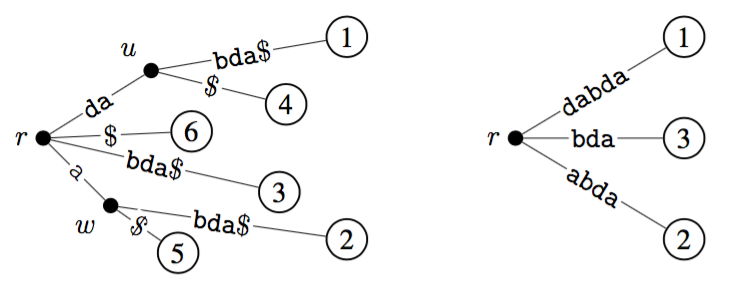
\includegraphics[width=.7\textwidth]{./notes/immagini/l19-fig2.png}
	\caption{Albero dei suffissi normale e implicito per la stringa $ S = dabda $.}
\end{figure}

L'algoritmo di Ukkonen costruisce un albero dei suffissi implicito $ I_i $ per ogni prefisso $ S[1,i] $ della stringa $ S\$ $ di lunghezza $ n+1 $ e incrementando \textit{i} finché non arriva a costruire $ I_{n+1} $. Siccome $ S[1,n+1] = S\$ $, l'albero dei suffissi implicito $ I_{n+1} $ coincide con l'albero dei suffissi \textit{A}, perché nessun suffisso della strina $ S\$ $ è prefisso di un altro suffisso.

\begin{breakablealgorithm}
	\caption{Ukkonen: Descrizione generale dell'algoritmo }
	\begin{algorithmic}[1]
		\Function{Ukkonen}{$S$}
			\State $ S \gets S\$ $ \Comment{Aggiunge la sentinella a $ S $}
			\State ``Costruisci $ I_0 $ ''
			\For{$ i = 0 \textbf{ to } n $}
				\For{$ j = 1 \textbf{ to } i+1 $}
					\State ``Cerca la fine del cammino relativo al suffisso $ S[j,i] $ in $ I_i $''
					\State ``Se necessario estendi il cammino con il carattere $S[i+1] $ in modo che il suffisso $ S[j,i] $ diventi un suffisso di $ S[1,i+1] $''
				\EndFor
			\EndFor
		\EndFunction
	\end{algorithmic}
\end{breakablealgorithm}

La costruzione di $ I_0 $ è banale in quanto contiene solo la radice e nessun arco uscente, perché la stringa $ S[1,0] $ ha come suffisso solamente $ \epsilon $.

Per costruire $ I_{i+1} $ è necessario modificare tutti i suffissi $ S[j,i] $ di $ S[1,i] $ nei suffissi $ S[j,i+1] $ di $ S[1,i+1] $.
Durante questa modifica possono verificarsi 3 casi:

\begin{enumerate}
	\item Il cammino etichettato $ S[j,i] $ termina in una foglia numerata $ j $. In questo caso il nuovo carattere $ S[i+1] $ viene aggiunto all'etichetta dell'ultimo arco del cammino (viene messo un nuovo nodo implicito).
	\item Il cammino etichettato $ S[j,i] $ termina in nodo interno \textit{u}, ma nessun cammino che parte da \textit{u} inizia con $ S[i+1] $. In questo caso viene creata una foglia etichettata $ j $ connessa al nodo \textit{u} con un arco etichettato $ S[i+1] $. Se \textit{u} è un nodo implicito, viene sostituito con un nodo esplicito, spezzando l'arco esistente.
	\item Il cammino etichettato $ S[j,i] $ termina in nodo interno \textit{u} e almeno un cammino che parte da \textit{u} è etichettato con $ S[i+1] $. In questo caso il suffisso $ S[j,i+1] $ è già presente nell'albero e non occorre fare niente.
\end{enumerate}

Dopo aver esteso tutti i suffissi di $ S[1,i] $ l'albero contiene tutti i suffissi di $ S[1,i+1] $, compreso il suffisso nullo che è sempre rappresentato.

\begin{figure}[htbp]
	\centering
	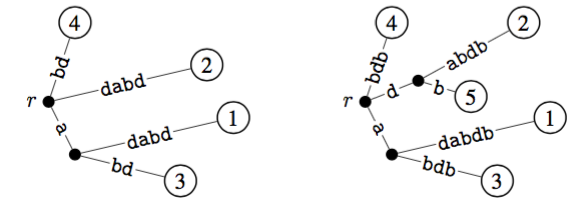
\includegraphics[width=.7\textwidth]{./notes/immagini/l19-fig3.png}
	\caption{Estensione dell'albero dei suffissi implicito per la stringa $ adabd $ quando si aggiunge alla stringa il carattere $ b $. I primi 4 suffissi vengono estesi con il caso 1, il quinto viene esteso con il caso 2 e il suffisso nullo viene esteso per il caso 3.}
\end{figure}

Tuttavia con questa implementazione si riesce a calcolare in $ O(i^2) $ l'albero $ I_{i+1} $ a partire da $ I_i $, portando ad una complessità totale di $ O(n^3) $ che è peggiore di quella dell'algoritmo naive.
 % Modello BM25
	% !TEX encoding = UTF-8
% !TEX TS-program = pdflatex
% !TEX root = computabilità e algoritmi.tex
% !TEX spellcheck = it-IT
\paragraph{Soluzione}\label{soluzione-esercizio}

La funzione \emph{f(x)} viene definita per casi e dal momento che i vari
predicati sono decidibili ed esaustivi, quindi almeno uno dei casi è
vero.

$$
f(\vec{x}) = f_1(\vec{x}))\cdot \mathcal{X}_{Q_1} + \ldots +	 f_m(\vec{x}))\cdot \mathcal{X}_{Q_m}
$$

Quando un caso è vero, viene calcolata la funzione associata, che è
totale. Se questa funzione non fosse totale, potrebbe essere che il
predicato vero su un certo \emph{x}, ma che la funzione su
quell'\emph{x} non sia definita e quindi neanche \emph{f(x)}
risulterebbe definita, perdendo così la totalità.

La calcolabilità deriva dal fatto che la definizione per casi viene
fatta con una serie di \emph{if} che è dimostrato essere calcolabile e
le funzioni $\mathcal{X}_{Q_i}$ sono calcolabili, perché i predicati sono
decidibili.

\subsubsection{Algebra della decidibilità}\label{algebra-della-decibilituxe0}

I predicati decidibili sono chiusi rispetto negazione, congiunzione e
disgiunzione.

Ovvero se \textit{Q} e \textit{Q'} sono due predicati in $\mathbb{N}^k$ decidibili allora anche:

\begin{enumerate}
\item $\neg Q(\vec(x))$
\item $ Q(\vec{x}) \wedge Q'(\vec{x})$
\item $ Q(\vec{x}) \vee Q'(\vec{x}) $
\end{enumerate}

Questo perché le relative funzioni che li calcolano possono essere definite come:

\begin{enumerate}
	\item $ \mathcal{X_{\neg Q}}(\vec{x}) = \overline{sg}( \mathcal{X_{Q}}(\vec{x})) $
	\item $ \mathcal{X_{Q \wedge Q'}}(\vec{x})= \mathcal{X_{Q}}(\vec{x}) \cdot \mathcal{X_{Q'}}(\vec{x})$
	\item $ \mathcal{X_{Q \vee Q'}}(\vec{x})= sg(\mathcal{X_{Q}}(\vec{x}) + \mathcal{X_{Q'}}(\vec{x}))$
\end{enumerate}

Tutte le funzioni così definite sono calcolabili perché ottenute da composizioni di funzioni calcolabili.

\subsubsection{Somma e prodotto dei valori di una funzione}

Data una funzione totale e $ f : \mathbb{N}^{k+1} \rightarrow  \mathbb{N}$ totale e calcolabile, è possibile definire le due funzioni che effettuano la somma e il prodotto dei primi \textit{y} valori della funzione.

\begin{align*}
	s(\vec{x}, y) &= \sum_{z < y} f(\vec{x},z) \\
	p(\vec{x}, y) &= \prod_{z < y} f(\vec{x},z) 
\end{align*}

Entrambe le funzioni sono calcolabili e totali perché possono essere definite induttivamente (ricorsivamente) a partire da delle funzioni calcolabili.

\begin{align*}
s(\vec{x}, y) &= \begin{cases} \sum_{z < 0}f(\vec{x},z) = 0, &\text{ se $ y = 0 $} \\
\sum_{z < y+1}f(\vec{x},z) = \sum_{z < y}f(\vec{x},z) + f(\vec{x},z), &\text{ altrimenti}
\end{cases} \\
p(\vec{x}, y) &=  \begin{cases} \prod_{z < 0}f(\vec{x},z) = 1, &\text{ se $ y = 0 $} \\
\prod_{z < y+1}f(\vec{x},z) = \prod_{z < y}f(\vec{x},z) \cdot f(\vec{x},z) &\text{ altrimenti}
\end{cases}
\end{align*}

La totalità deriva dal fatto che \textit{f} è totale.

\subsubsection{Quantificazione limitata}

Combinando algebra della decidibilità e quanto detto nel paragrafo precedente è possibile la decidibilità di $ \forall $ e $ \exists $.

Dato un predicato $ Q(\vec{x},z) $ per calcolare se $ \forall z < y, Q(\vec{x},z) $ è possibile utilizzare la funzione:

$$
\mathcal{X}_{Q_\forall} = \prod_{z < y} \mathcal{X}_Q(\vec{x},z)
$$

In modo simile è possibile calcolare $ \exists z < y, Q(\vec{x},z) $:

$$
\mathcal{X}_{Q_\exists} = sg(\sum_{z < y} \mathcal{X}_Q(\vec{x},z))
$$

Trattandosi della composizione di funzioni calcolabili e totali, le funzioni così ottenute sono a loro volta calcolabili e totali.

\section{Minimalizzazione limitata}

Data una funzione $ f(\vec{x},z) : \mathbb{N}^{k+1} \rightarrow \mathbb{N}$ calcolabile e totale è possibile definire una funzione 

$$
h(\vec{x},y) = \mu z< y | f(\vec{x},z) = 0
$$

$ h $ è ancora una funzione $ \mathbb{N}^{k+1} \rightarrow \mathbb{N} $ e viene calcolata come il minimo valore di \textit{z} minore di \textit{y} e tale che $ f(\vec{x},z) $ sia uguale a 0 (tipicamente l'uguale a 0 viene omesso). 

La definizione più precisa è:

$$
h(\vec{x}, y) = \mu z < y . f(\vec{x},z) = \begin{cases}
\text{minimo $ z < y $ tale che $f(\vec{x},z) = 0$ se questo esiste} \\
y, \text{altrimenti}
\end{cases}
$$

Per come è definita, questa funzione risulta essere \textbf{totale} e \textbf{calcolabile}.
Intuitivamente è calcolabile perché si tratta di calcolare \textit{f} per vari valori, serve però una dimostrazione più formale, fatta per ricorsione primitiva.

\begin{align*}
	h(\vec{x}, 0) &= 0\\
	h(\vec{x}, y+1) &= 	\begin{cases}
										h(\vec{x},y) < y, &\text{\textit{f} si annulla su un valore minore di \textit{y}, viene resituito $ h(\vec{x},y) $}\\
										h(\vec{x},y) = y, &\text{per tutti i valori di minori \textit{y} non c'è uno 0 } \begin{cases}
										\text{se } f(\vec{x},y) = 0 \rightarrow y \\ 
										\text{se } f(\vec{x},y) \neq 0 \rightarrow y+1
										\end{cases}
										\end{cases}
\end{align*}

La seconda parte può essere facilmente tradotta nell'espressione

$$
(y \dotminus h(\vec{x},y)) \cdot (h(\vec{x},y)) + \overline{sg}(y \dotminus h(\vec{x},y)) \cdot (y + sg(f(\vec{x},y)))
$$

Dal momento che la funzione \textit{h} può essere definita per ricorsione primitiva e per composizione di funzioni calcolabili, anche lei è calcolabile.

\subsection{Funzioni calcolabili per ricorsione limitata}

Utilizzando la ricorsione limitata è possibile dimostrare la calcolabilità di varie funzioni.

\subsubsection{Numero di divisori di $x$}

\begin{align*}
	D(x) &= \text{\# divisori di } x \\
			&= \sum_{y \leq x}(\overline{sg}(rm(y,x))) 
\end{align*}

Dove \textit{rm} è la funzione resto, precedentemente dimostrata calcolabile.

\subsubsection{Numeri primi}

Dimostrare la calcolabilità dei funzioni che lavorano con i numeri primi è importante perché torneranno utili in futuro.

\begin{align*}
	Pr(x) &= \text{``$x$ è primo ''} \\
			 &= \overline{sg}(|D(x) - 2|)
\end{align*}

\begin{align*}
	P_x &= \text{``$x$-esimo numero primo, per convezione: ''} P_0 = 0, P_1 = 2, \ldots \\
	&= \begin{cases}
	P_0 = 0& \\
	P_{x+1} = \mu z \leq (P_x! + 1) \: | Pr(z) \cdot \underbrace{\overline{sg}(P_x +1 \dotminus z)}_{1 \text{ se } z > P_x  } \dotminus 1| &
	\end{cases}
\end{align*}

\begin{align*}
	(x)_y 	&= \text{esponente di  } P_y \text{ nella decomposizione di } y \\
			   &= \text{max } z \: P_{y}^z \text{ divide } x \rightarrow \mu z \leq x \text{ tale che } P_{y}^{z+1} \text{ non divide } x \\
			   &= \mu z \leq x \: \overline{sg}(rm(P_{y}^{z+1},x))
\end{align*}

\subsubsection{Esercizio - mcm, MCD, radice di x}

Dimostrare che sono calcolabili:

\begin{itemize}
	\item $ floor(\sqrt{x}) $
	\item $mcm(x,y))$
	\item $MCD(x,y)$
\end{itemize}


\section{Codifica di coppie}

La funzione di \textit{fibonacci} non può essere definita per ricorsione primitiva, perché il passo induttivo richiede una coppia di valori precedenti.

\`{E} però possibile definire una funzione $\prod : \mathbb{N} \times \mathbb{N} \rightarrow \mathbb{N}$ che codifica il valore di una coppia in un unico numero:

$$
\prod (x,y) = 2^x(2y+1) \dotminus 1
$$

Questa funzione risulta essere biunivoca perché è possibile definire l'inversa:

$$
\prod^{-1}(x) = ((n+1)_1, \frac{1}{2}(\frac{n+1}{(n+1)_1})-1)
$$

La funzione inversa è effettiva, perché è definita in termini di componenti calcolabili, anche se la definizione di funzione calcolabile non è stata vista per funzioni $\mathbb{N} \rightarrow \mathbb{N} \times \mathbb{N}$.

Utilizzando la funzione accoppiamento, è possibile definire la funzione \textit{fib} per ricorsione primitiva:

\begin{align*}
	g(x) &= \prod(fib(x), fib(x+1)) \\
	g(0) &= \prod(fib(0), fib(1)) = \prod(1,1) = 5 \\
	g(x+1) &= \prod(fib(x+1), fib(x+2)) \\
				 &= \prod(fib(x+1, fib(x)+fib(x+1)) \\
				 &= \prod(\prod_2(g(x)),\prod(\prod_1(g(x))+\prod_2(g(x)))\\		 
\end{align*}

Dove $\prod_1$ e $\prod_2$ sono rispettivamente le funzioni per il calcolo del primo e del secondo elemento della coppia.

Così facendo è stata dimostrata la calcolabilità di \textit{g} per ricorsione primitiva, ma $fib(x) = \prod_1(g(x))$ e di conseguenza \textit{fib} è calcolabile per composizione di funzioni calcolabili.

\section{Minimalizzazione illimtata}

Data $ f : \mathbb{N}^{k+1} \rightarrow \mathbb{N} $, si vuole definire $ h : \mathbb{N}^k \rightarrow \mathbb{N} $ tale che calcoli il minimo \textit{z} che azzera la funzione \textit{f}, ovvero:

$$
h(\vec{x}) = \mu z.f(\vec{x},z)
$$

Ci sono però dei problemi se $ f(\vec{x}, z) $ è sempre diversa da zero, perché in questo caso $ h $ è $ \uparrow $.

Un altro problema si ha se la funzione è indefinita per un valore $ z' $ minore dello $ z $ che azzera la funzione. Anche in questo caso si ha che $ h $ è $ \uparrow $.

$$
h(\vec{x}) = \mu z.f(\vec{x},z) = \begin{cases}
\text{minimo \textit{z} tale che } f(\vec{x},z) = 0 \text{ se esiste e se } \forall z' < z, f(\vec{x},z')\downarrow \neq 0 \\
\uparrow \text{ altrimenti}
\end{cases}
$$

Alternativamente, definendo $ Z_{f, \vec{x}} = \{z | f(\vec{x},z) = 0 \wedge \forall z' < z f(\vec{x},z') \downarrow \} $, si ha che \textit{h} è definita come

$$
h(\vec{x}) = \begin{cases}
\min Z_{f,\vec{x}} \text{ se } Z_{f,\vec{x}} \neq \emptyset \\
\uparrow \text{ altrimenti}
\end{cases}
$$

\subsection{Esercizi}

\subsubsection{Esercizio - Radice quadrata}
Dimostrare la calcolabilità di 

$$
f(x) = \begin{cases}
\sqrt{x} \text{ se \textit{x} è un quadrato} \\
\uparrow \text{ altrimenti}
\end{cases}
$$

\paragraph{Soluzione}

L'idea è quella di trovare un \textit{y} che elevato al quadrato è uguale a \textit{x}: $ y^2 - x = 0 $.

Si ha quindi che

$$ 
f(x) = \mu y.|y^2-x|
$$

ed è calcolabile perché minimizza illimitatamente una composizione di funzione calcolabile.

\subsubsection{Esercizio teorico}

Dimostrare che se $ f : \mathbb{N} \rightarrow \mathbb{N} $ è iniettiva, calcolabile e totale, anche la sua inversa è calcolabile.

\paragraph{Soluzione}

$$
f^{-1}(x) = \begin{cases}
y, &\text{ tale che } f(y) = x \\
\uparrow, &\text{ altrimenti}  
\end{cases}
$$

$$ 
f^{-1}(x) = \mu y.|f(y)-x|
$$

Perché l'uguaglianza sia rispettata è necessario che \textit{f} sia totale, dal momento che se per un certo \textit{y}, \textit{f} non è definita il programma che la calcola non termina, rendendo indefinita anche $ f^{-1} $.

C'è un barbatrucco per gestire anche la non totalità di \textit{f}, ovvero quello di eseguire contemporaneamente il calcolo per ogni \textit{y}, eseguendo tot passi alla volta per ognuno dei calcoli (\textit{dovrebbe essere dimostrato in futuro}).

Dal momento che \textit{f} è calcolabile si ha che anche l'inversa è calcolabile per minimizzazione illimitata di una composizione di funzioni calcolabili.

L'iniettività\footnote{Una funzione $ f: X\rightarrow Y $ si dice iniettiva se due elementi distinti del dominio hanno immagini distinte, ovvero $a_1\neq a_2$ implica $f(a_1)\neq f(a_2)$.} garantisce che il valore trovato sia quello corretto.


\subsubsection{Esercizio - Divisione}

$$
f(x,y) = \begin{cases}
\frac{x}{y}, &\text{ se } y \neq 0 \text{ e \textit{x} divisibile per \textit{y}}\\
\uparrow, &\text{altrimenti} 
\end{cases}
$$

\paragraph{Soluzione}

$$
f(x,y) = \mu k. |x \dotminus y\cdot k|
$$

C'è però un problema, perché la funzione così definita risulta calcolabile se \textit{x} e \textit{y} sono uguali a 0.

$$
f(x,y) = \mu k.(|x - y\cdot k| + \underbrace{\overline{sg}(y)}_{\text{vale 1 se \textit{y} è uguale a 0}})
$$

Così facendo se $ y=0 $ la minimalizzazione non converge.

Questo porta ad un discorso un po' più ampio sulla possibilità di aggiustare una funzione che si comporta quasi come un'altra funzione (§\ref{hotfix}).

	\section{Lezione 13 - Support Vector Machine}\label{lezione-13---support-vector-machine}

Nelle precedenti puntate:

\begin{itemize}
\item
  Sappiamo che un iperpiano in uno spazio di dimensione \textit{m} ha VC
  dimension \textit{m+1}.
\item
  Si può aggiungere un vincolo di classificazione relativo al margine.
\item
  Per ottenere l'iperpiano con margine ottimo è necessario considerare
  l'ipotesi che minimizza la norma di \emph{w}.
\item
  Il tutto si fa con un polinomio di Lagrange e il suo duale.
\end{itemize}

\subsection{Dati non separabili linearmente}\label{dati-non-separabili-linearmente}

Tutto quello visto finora funziona se i dati sono linearmente
separabili.

Nel caso questi non lo siano è necessario permettere che alcuni vincoli possano essere violati e per fare ciò vengono introdotte delle nuove variabili $\xi_i \geq 0$, una per ogni vincolo (ovvero per ogni esempio del training set), tale che:

$$ y_i (\vec{w} \cdot \vec{x}_i + b) \geq 1 - \xi_i $$

Queste nuove variabili rappresentano la distanza dell'esempio \textit{i}-esimo dal margine.

\begin{figure}[htbp]
\centering
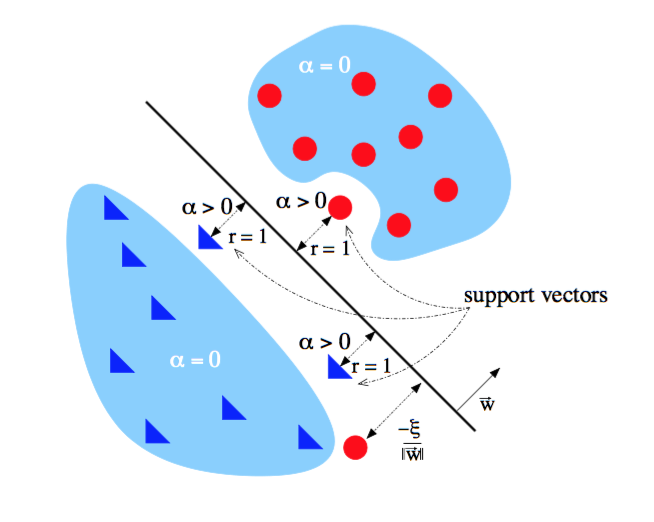
\includegraphics[width = 0.6\textwidth]{./notes/immagini/l13-non-linear.png}
\caption{SVM con dati non linearmente separabili.}
\end{figure}

L'idea è quindi quella di andare a sommare alla funzione costo la sommatoria di tutti i $\xi_i$ dei vari esempi presenti nel training set, moltiplicata per un coefficiente di penalizzazione \textit{C} che rappresenta un iper-parametro dell'algoritmo di apprendimento, da ottimizzare con le tecniche di model selection.

La nuova formula da minimizzare diventa:

$$ \frac{1}{2}||\vec{w}||^2 + C \sum\limits_{i=1}^n \xi_i $$

In pratica vengono penalizzati (aumentato il costo) gli esempi che non rispettano il margine.

La minimizzazione avviene considerano il problema duale, che risulta essere definito come:

$$max_\alpha \sum\limits_{i=1}^n \alpha_i - \frac{1}{2}\sum\limits_{i,j = 1}^n y_i y_j \alpha_i \alpha_j (\vec{x}_i \cdot \vec{x}_j)$$

$$ \text{s.t.: } \forall i \in \{1, \ldots, n\} : 0 \leq \alpha_i \leq C \text{ e } \sum\limits_{i=1}^n y_i \alpha_i = 0$$

Da notare che le $\xi_i$ sono variabili del problema primale e che quindi non compaiono nel problema duale.

Questa strategia per esempi non linearmente separabili non sempre
garantisce buone prestazioni perché un iper-piano può solo rappresentare
dicotomie dello spazio delle istanze.

Per questo motivo, quando gli esempi non sono linearmente separabili su
usa una strategia divisa in due passi:

\begin{enumerate}
\item
  Si mappano i dati di ingresso (input space) in uno spazio a dimensione
  molto superiore (feature space). Quindi a partire dalle feature degli
  elementi dell'input space vengono creati nuovi esempi nel feature
  space che utilizza combinazioni non lineari delle feature del primo
  spazio.
\item
  Si calcola poi l'iper-piano ottimo per il nuovo spazio usando la
  formulazione precedente (che prende il nome di variabili slack).
\end{enumerate}

Perché dovrei farlo?

\begin{enumerate}
\item
  Perché il \textbf{teorema sulla separabilità di Cover} afferma che un problema di classificazione complesso, formulato
  attraverso una trasformazione non lineare dei dati in uno spazio ad
  alta dimensionalità, ha maggiore probabilità di essere linearmente
  separabile che in uno spazio a bassa dimensionalità.
\item
  Perché l'iper-piano ottimo minimizza la VC-Dimension e quindi la
  capacità di generalizzazione migliora.
\end{enumerate}

Viene quindi utilizzata una trasformazione $\varphi(\cdot)$ non lineare, da applicare ai dati originari del problema $\{(\vec{x}_i, y_i)\}_1^n$ tale che:

$$ \forall i \: \vec{x}_i \in R^m, \varphi(\vec{x}_i) = \vec{Z}, \vec{Z} \in R^M, M \gg m $$

Il vettore ottenuto può essere rappresentato come $\vec{\varphi}(\vec{x}) = [ \varphi_1(\vec{x}), \ldots , \varphi_M(\vec{x}) ] $.

Con questa notazione è possibile andare a definire l'iper-piano nel nuovo spazio con:

$$ \sum\limits_{j=1}^M w_j \varphi_j(\vec{x}) + b = 0$$

che se si considera il termine noto $b = w_0$ e si aggiunge $\varphi_0(\vec{x}) = 1$, risulta essere

$$ \sum\limits_{j=0}^M w_j \varphi_j(\vec{x}) = \vec{w} \cdot \vec{\varphi}(\vec{x}) = 0$$

Andando a sostituire il $\vec{w}$ dell'equazione precedente con $ \vec{w} = \sum\limits_{k=1}^n j_k \alpha_k \vec{\varphi}(\vec{x}_k)$ si ottiene:

$$ \sum\limits_{k=1}^n j_k \alpha_k \varphi(\vec{x_k}) \cdot \varphi(\vec{x}) = 0 $$

Con il termine $\varphi(\vec{x}_k) \cdot \varphi(\vec{x})$ rappresenta il prodotto scalare tra un vettore del training set $\vec{x}_k$ e il vettore in input $\vec{x}$ calcolato nello spazio $R^M$.

\subsection{Funzioni Kernel}\label{funzioni-kernel}

Lo spazio di dimensione superiore serve solo per calcolare il prodotto scalare tra i due vettori, si può quindi definire una funzione $K(\cdot, \cdot)$ che prende il nome di kernel e che calcola il prodotto scalare dei due vettori senza passare esplicitamente nello spazio di dimensione superiore.

$$ K(\vec{x}_k, \vec{x}) = \varphi(\vec{x}_k) \cdot \varphi(\vec{x})$$

Assumendo di avere una di queste funzioni, l'iper-piano risulta essere:

$$\sum\limits_{k=1}^n  y_k \alpha_k K(\vec{x}_k, \vec{x}) = 0$$

Per il teorema di Mercer esistono delle funzioni di questo tipo, ma è necessario che soddisfino determinate condizioni.

Alcune di queste sono:

\begin{itemize}
\item \textbf{Polinomiale di grado \textit{p}}: $K(\vec{x},\vec{y}) = (\vec{x} \cdot \vec{y} +1) ^p$
\item \textbf{RBF}: $ K(\vec{x},\vec{y}) = exp(-\frac{1}{2\sigma^2}||\vec{x}-\vec{y}||^2)$
\end{itemize}

La formulazione duale del problema risulta quindi essere:

$$max_\alpha \sum\limits_{i=1}^n \alpha_i - \frac{1}{2}\sum\limits_{i,j = 1}^n y_i y_j \alpha_i \alpha_j K(\vec{x}_i ,\vec{x}_j)$$

$$ \text{s.t.: } \forall i \in \{1, \ldots, n\} : 0 \leq \alpha_i \leq C \text{ e } \sum\limits_{i=1}^n y_i \alpha_i = 0$$

Per fare la classificazione viene utilizzato il \textbf{segno} della funzione:

\begin{align*}
f(\vec{u})  &= \sum\limits_{i = 1}^n y_i  \alpha_i  K(\vec{x}_i,  \vec{u}) + b
\end{align*}

\subsection{Regressione}\label{regressione}

Quando si considera il problema di approssimazione di funzioni a valori
reali (regressione) si utilizza l'$\epsilon$-tubo: output che differiscono dai
valori di target per più di $\epsilon$ in valore assoluto vengono penalizzati
linearmente, altrimenti non vengono considerati errori. In pratica
aggiungo un intervallo di tolleranza al iper-piano che partiziona lo
spazio.

\begin{figure}[htbp]
\centering
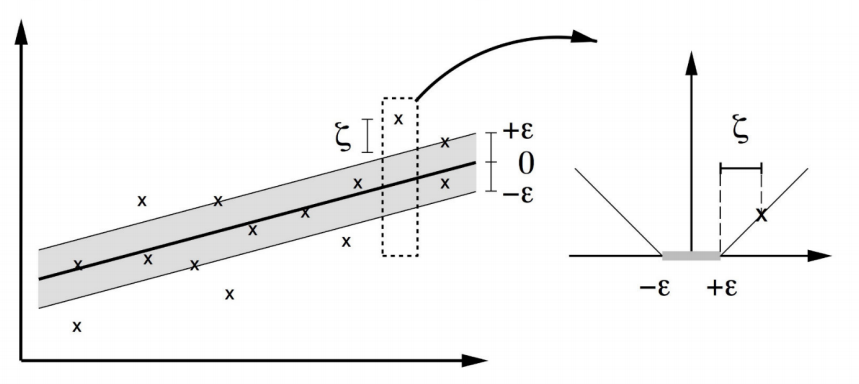
\includegraphics[width = 0.8\textwidth]{./notes/immagini/l13-primale-duale.png}
\caption{Regressione in forma primale (a sinistra) e duale (a destra)}
\end{figure}

\todo[inline]{Mancano formule (ultime due slide) http://www.math.unipd.it/\~{}aiolli/corsi/1516/aa/SVM.pdf}
	% !TEX encoding = UTF-8
% !TEX program = pdflatex
% !TEX root = MEMOC.tex
% !TEX spellcheck = it-IT

% 15 Dicembre 2016

\todo[inline]{Da recuperare}
	\section{Lezione 15 - Apprendimento Bayesiano}\label{lezione-15---apprendimento-bayesiano}

Si tratta di algoritmi di apprendimento basati sulla probabilità e sul
teorema di Bayes che effettuano la classificazione utilizzando l'ipotesi che
più probabilmente approssima la funzione target, scegliendola da un'insieme di funzioni $H$.

\subsection{Scelta delle ipotesi}\label{scelta-delle-ipotesi}

Tutto si basa sulla formula di Bayes.

$$
P(h | D) = \frac{P(D|h)P(h)}{P(D)}
$$

Dove:

\begin{itemize}
\item $P(h)$ è la probabilità a priori che l'ipotesi \textit{h} sia corretta e rispecchia la conoscenza a priori che si ha sul dominio;
\item $P(D)$ è la probabilità a priori che vengano osservati i dati \textit{D};
\item $P(h|D)$ è la probabilità che l'ipotesi \textit{h} sia corretta per i dati \textit{D};
\item $P(D|h)$ è la probabilità che i dati \textit{D} vengano classificati correttamente da \textit{h} \end{itemize}

L'obiettivo è quello di massimizzare \emph{P(h\textbar{}D)}, sapendo
\emph{P(D\textbar{}h)} che viene fornito dal supervisore e \emph{P(h)}
che viene appresa.

Nel massimizzare si può tralasciare il termine \emph{P(D)} dal momento
che è sempre costante.

$$
h_{MAP} = argmax_{h \in H} P(D|h)P(h)
$$

$H_{MAP}$ prende il nome di \textbf{ipotesi massima a posteriori}.

Si può inoltre assumere che tutte le ipotesi \emph{h} abbiano la stessa probabilità a priori, e nel mondo reale questa assunzione è tipicamente corretta, il
problema di massimizzazione diventa:

$$
h_{ML} = argmax_{h \in H} P(D|h)
$$

In questo caso si sceglie l'ipotesi di \textbf{maximum likelihood}

A pagina 158 del Mitchel c'è un esempio che mette in evidenza come le
probabilità a priori influenzino il risultato.

\subsection{Brute Force MAP Learning (interpretazione Find-S)}\label{brute-force-map-learning-interpretazione-find-s}

L'apprendimento dell'ipotesi massima avviene adattando l'algoritmo Find-S per l'apprendimento di concetti.

Si assumono fissate le istanze $x_1, \ldots, x_n$ e \textit{D} essere l'insieme dei valori desiderati $D = \{ c(x_1), \ldots, c(x_n)\}$.

Considerando inoltre tutte le ipotesi equiprobabili: $P(h) = \frac{1}{|H|}$, si ha che:

$$
P(D|h) = 
	\begin{cases}
		1,& \text{ se \textit{h} è consistente con \textit{D}} \\
		0,& \text{ altrimenti }
	\end{cases}
$$

L'algoritmo di apprendimento risulta quindi essere:

\begin{enumerate}
\item Per ogni potesi $h \in H$ calcola $P(h|D)$;
\item Scegli l'ipotesi che massimizza $P(h|D)$.
\end{enumerate}

Se i dati di apprendimento sono senza rumore e se la funzione target è contenuta nello spazio delle ipotesi \textit{H}, è possibile calcolare \emph{P(h\textbar{}D)} applicando la regola di Bayes, in particolare:

$$
P(h|D) = 
	\begin{cases}
		\frac{1}{|VS_{H,D}|},& \text{ se \textit{h} è consistente con \textit{D}} \\
		0,& \text{ altrimenti }
	\end{cases}
$$

Quindi se tutte le ipotesi \emph{h} sono equiprobabili, allora qualsiasi
ipotesi presente in \emph{H} va bene con probabilità $\frac{1}{VS_{H,D}}$, dove $VS_{H,D}$ è un sottoinsieme di \textit{H} consistente con \textit{D}.

Con questa definizione, tutte le ipotesi consistenti hanno probabilità $\frac{1}{VS_{H,D}}$ e tutte quelle non consistenti hanno probabilità \textit{0}, pertanto tutte le ipotesi consistenti possono essere delle $h_{MAP}$.

Segue anche che l'algoritmo Find-S ritorna sempre $h_{MAP}$ anche se non vengono utilizzate esplicitamente le probabilità.

Se vengono cambiate le probabilità in modo che la probabilità di
un'ipotesi più specifica sia più alta si ottiene che
\emph{P(h\textbar{}D) = P(h)}.

\subsection{Apprendimento di una funzione (ML)}\label{apprendimento-di-una-funzione-ml}

Si vuole apprendere una funzione $f$ a valori reali, utilizzando come esempi di apprendimento $(x_i, d_i)$ dove il valore target $d_i$ può contenere del rumore:

$$
d_i = f(x_i) + e_i
$$

dove $e_i$ è l'errore che segue una probabilità gaussiana con media 0 di
cui non si conosce la varianza.

Però si vuole valutare l'errore come se al posto di \emph{f} (che è sconosciuta) ci fosse \emph{h}

$$
e_i = d_i - h(x_i)
$$

La probabilità di $P(d_i | h)$, cioè che l'ipotesi \emph{h}
classifichi correttamente $d_i$ segue la distribuzione guassiana di
$e_i$.

Dalla definzione di ipotesi \textit{maximum likelihood} si ottiene che l'ipotesi $h_{ML}$ è anche quella che minimizza il quadrato degli errori:

\begin{align*}
h_{ML} &= argmax_{h \in H} P(D|h) \\
				&=  argmax_{h \in H} \prod\limits_{i=1}^m P(d_i|h) \\
				&= *\textit{gauassia di } e_i \textit{, logaritmi e altra math-magic*}\\
				&= arg min_{h \in H} \sum\limits_{i = 1}^m (d_i - h(x_i))^2
\end{align*}

Quindi per trovare l'ipotesi \textbf{maximum likelihood} è necessario
minimizzare l'errore quadratico, sotto l'ipotesi che la probabilità di
ogni ipotesi è uniforme e assumendo che i dati di apprendimento $d_i$ contengano del rumore che segue la distribuzione guassiana con media 0.

L'ipotesi \textit{MAP} coincide con l'ipotesi \textit{ML} solo se tutte le ipotesi hanno probabilità uniforme.

C'è anche da tenere in considerazione che questo approccio assume del rumore solamente nei dati $d_i$ e non dei vari $x_i$.

\subsection{Ipotesi MDL}

La scelta di questa ipotesi segue il principio del rasoio di Occam:``\textit{scegli la spiegazione più semplice per i dati osservati}'', ovvero sceglie l'ipotesi:

$$
h_{MDL} = argmin_{h \in H} L_{C_1}(h) + L_{C_2}(D|H)
$$

dove $L_C(x)$ è la lunghezza della descrizione di \textit{x} nella codifica \textit{C}.

Ad esempio, sfruttando la teoria dell'informazione è possibile utilizzare:

\begin{itemize}
\item $L_{C_1}(h) = - log_2(P(h))$
\item $L_{C_2}(D|h) = - log_2(P(D|h))$
\end{itemize}

Con questa codifica si ottiene che

\begin{align*}
h_{MDL} 	&= argmin_{h \in H} L_{C_1}(h) + L_{C_2}(D|H) \\
				&= argmin_{h \in H} - log_2(P(h)) - log_2(P(D|h)) \\
				&= argmax_{h \in H} P(D|h)P(h) \\
				&= h_{MAP}
\end{align*}

Ovvero che \textit{MDL} coincide con \textit{MAP}.

L'idea alla base di questo approccio è quella di effettuare un trade-off tra la complessità dell'ipotesi e il numero di errori commessi. L'ipotesi \textit{MDL} commette più errori sui dati di apprendimento a causa della sua brevità, ma ciò può essere visto come una limitazione dell'overfitting.

\subsection{Classificazione}\label{classificazione}

Finora abbiamo cercato l'ipotesi più probabile per i dati \emph{D}
($h_{MAP}$), ma dato un nuovo esempio, qual'è la classificazione più
probabile? Non sempre l'idea migliore è quella di calcolare $h_{MAP}(x)$.

Supponiamo di avere 3 ipotesi tali che: \emph{P($h_1$\textbar{}D)=0.4},\emph{P($h_2$\textbar{}D)=0.3},
\emph{P($h_3$\textbar{}D)=0.3} e che data una nuova istanza \emph{x} può si ottiene \emph{$h_1$(x) = (+)} e \emph{$h_2$(x) = $h_3$(x) = (-)}. 

In questo caso $h_{MAP}$, ovvero $h_1$, fornisce come classificazione $(+)$, anche se la classificazione più probabile è $(-)$.

Il \textbf{classificatore ottimo di Bayes} si basa su questo principio e classifica una nuova istanza $x$ con l'etichetta:

$$
v_x = argmax_{v_j \in V} \sum\limits_{h_i \in H} P(v_j | h_i)P(h_i | D)
$$

Dove:

\begin{enumerate}
\item $V$ è l'insieme di tutte le possibili classi
\item $
P(v_j | h_i) = 
	\begin{cases}
		1,& \text{ se } h_i(x) = v_j \\
		0,& \text{ altrimenti }
	\end{cases}
$
\end{enumerate}

Utilizzando lo stesso spazio delle ipotesi e la stessa conoscenza a priori, nessun altro classificatore riesce a superare il classificatore ottimo di Bayes.

Tuttavia, ad ogni classificazione è necessario calcolare la classificazione effettuata da ogni ipotesi $h_i$ e questo può essere computazionalmente oneroso al crescere del numero di ipotesi.

\subsection{Classificatore di Gibbs}\label{classificazione-di-gibbs}

Un'alternativa sub-ottima al classificatore di Bayes è data dall'algoritmo di Gibbs:

\begin{enumerate}
\item Sceglie un'ipotesi $h$ a caso, secondo $P(h|D)$,
\item utilizza l'ipotesi scelta per classificare l'istanza.
\end{enumerate}

Il classificatore così ottenuto è semplice da calcolare e funziona sorprendentemente bene dal momento che l'errore medio che compie è minore del doppio dell'errore effettuato dal classificatore ottimo:

$$
E[errore_{Gibbs}] \leq 2E[errore_{BayesOttimo}]
$$

Sempre assumendo probabilità a priori uniforme per tutte le ipotesi del version space.
	\subsubsection{Calcolabilità della minimalizzazione}\label{calcolabitliuxe0-della-minimalizzazione}

Se $ f : \mathbb{N}^{k+1} \rightarrow \mathbb{N} $ è in $ \mathcal{C} $, allora anche
$\mu y.f(\vec{x},y)$ è in $ \mathcal{C} $.

\paragraph{Dimostrazione}\label{dimostrazione}

Sia  $ f : \mathbb{N}^{k+1} \rightarrow \mathbb{N} $ in $ \mathcal{C} $ e sia \textit{P} il programma in
forma normale che calcola \textit{f}.

L'idea è quella di eseguire \emph{P} incrementando via via un contatore e, quando viene trovato un valore del contatore che azzera la funzione, questo viene ritornato.

\begin{verbatim}
 1       k         m+1          m+k|m+k+1|m+k+2|
|\vec{x} | .....  |x_1|x_2|....|x_k|  0  |  0  |
\end{verbatim}

Sia $m = \max{\rho(P), k }$, il programma che calcola la minimalizzazione illimitata è:

\begin{lstlisting}[language=URM]
T([1..k], [m+1..m+k]) //Copio l'input
P[m+1, ..., m+k+1 -> 1]
J(1, m+k+2, END) #LOOP
S(m+k+1)
J(1,1,LOOP)
#END
\end{lstlisting}

Dal momento che è possibile trovare un programma che calcola la
minimalizzazione illimitata, questa è calcolabile.

\subsubsection{Hot-fix delle funzioni} \label{hotfix}
Data una funzione  $ f : \mathbb{N} \rightarrow \mathbb{N} $ tale che esiste  $ g : \mathbb{N} \rightarrow \mathbb{N} $ calcolabile e tale che

$$
\Delta = \{ x | f(x) \neq g(x) \}
$$

e finito.

Allora \emph{f} è calcolabile e può essere modificata in modo da
coincidere con \emph{g}.

\subsubsection{Funzioni finite}\label{funizioni-finite}

\textbf{Funzione finita} $ \Theta: \mathbb{N}^{k} \rightarrow \mathbb{N}  $è una funzione
finita quando è definita come:

$$
\Theta(\vec{x}) = \begin{cases}
y_1, &\text{ se } \vec{x} = \vec{x}_1 \\
y_2, &\text{ se } \vec{x} = \vec{x}_2 \\ 
\cdots \\
y_n, &\text{ se } \vec{x} = \vec{x}_n \\
\uparrow, &\text{ altrimenti}
\end{cases}
$$

Tutte le funzioni di questo tipo sono calcolabili

\paragraph{Dimostrazione}\label{dimostrazione-1}

(per semplicità è ridotta a funzione unarie)

\begin{align*}
\Theta &= \begin{cases}
y_1, &\text{ se } x = x_1 \\
y_2, &\text{ se } x = x_2 \\ 
\cdots \\
y_n, &\text{ se } x = x_n \\
\uparrow, &\text{ altrimenti}
\end{cases} \\
&= y_1 \cdot \overline{sg}(|x - x_1|) + \cdots + y_n \cdot \overline{sg}(|x - x_n|) +  \underbrace{\mu z.\prod\limits_{i=1}^{n}|x - x_i|}_{\text{funzione indipendente da } z}
\end{align*}

La minimalizzazione su \emph{z} è calcolabile ma risulta indefinita, perché non è possibile minimizzarla rispetto a \emph{z}, quindi anche la funzione $ \Theta $ risulta essere indefinita se tutti i valori sono diversi da $ x_1 \ldots x_n $.

\section{Tesi di Church}\label{tesi-di-church}

Ogni funzione è calcolabile tramite un procedimento effettivo se e solo
se è URM calcolabile.

Church non ha proprio detto questo, perché non c'era URM quando è stata
enunciata e ha utilizzato un modello alternativo: le funzioni parziali
ricorsive $ \mathcal{R} $ (G\"{o}edel).

La classe $ \mathcal{R} $ delle \textbf{funzioni parziali ricorsive} è la \textbf{minima} classe di funzioni che contiene:

\begin{enumerate}[(a)]
\item  zero: $ z(\vec{x}) = 0 $ per ogni \textit{x}
\item  successore: $ S(x) = x+1 $
\item  proiezioni: $ U_{i}^k (x_1 \ldots x_k) = x_i $
\end{enumerate}

ed è chiusa rispetto:

\begin{enumerate}
\item
  composizione generalizzata
\item
  ricorsione primitiva
\item
  minimalizzazione illimitata.
\end{enumerate}

Una classe di funzioni \emph{X} è \textbf{ricca} se contiene le funzioni
di base ed è chiusa rispetto alle 3 operazioni classiche.

C'è almeno una classe ricca, perché anche la classe ``tutte le
funzioni'' è ricca, anche se ha poco senso considerarla.

Si vuole quindi che $ \mathcal{R} $ sia contenuta in \emph{X} ricca e che anche
$ \mathcal{R} $ sia ricca.

Questo è possibile perché l'intersezione di due classi ricche è
ovviamente anch'essa ricca.

$ \mathcal{R} $ può essere definita come l'intersezione di tutte le classi di
funzioni ricche.

$$
\mathcal{R} = \bigcap_{X \text{ ricca}} X
$$

anche se precedentemente $ \mathcal{R} $ è stata definita come

$$
\mathcal{R} = \{ (a), (b), (c) \text{ con tutte le funzioni che si ottengono da queste utilizzando } 1,2,3 \}
$$

È dimostrabile che le due definizioni sono equivalenti, anche se non lo
dimostriamo.

Si può anche definire la classe $ \mathcal{PR} $ delle \textbf{funzioni
primitive ricorsive}: la minima classe che contiene solamente le funzioni
di base chiusa rispetto la composizione e la ricorsione primitiva.
Ovviamente $ \mathcal{PR} $ è più piccola di $ \mathcal{R} $.

\subsection{$ \mathcal{C} $ = $ \mathcal{R} $}\label{c-figa-r-figa}

È già stato dimostrato che $ \mathcal{C} $ è una classe ricca, quindi sicuramente
$ \mathcal{R} \subseteq \mathcal{C} $.

Resta da dimostrare che $ \mathcal{C} \subseteq \mathcal{R} $.

Sia \textit{f} in $ \mathcal{C} $, ovvero esiste un programma \emph{P} in forma normale
che la calcola $f = f_p^{(k)}$.

\begin{verbatim}
P= I_1 ... I_s

|x_1 ... x_k| 0 ... 0
\end{verbatim}

Supponiamo di avere le funzioni:

$$
C_{p}^1(\vec{x},y) = \begin{cases}
\text{contenuto di R1 dopo \textit{t} passi del programma se non è terminato} \\
\text{altrimenti ritorna il valore finale del registro}
\end{cases} 
$$

$$
J_p(\vec{x},t) = \begin{cases}
\text{la prossima istruzione da eseguire all'istante \textit{t} di } P(\vec{x}) \text{ se non è terminato}\\
0 \text{ altrimenti }
\end{cases}
$$

Si ha che entrambe le funzioni sono del tipo $\mathbb{N}^{k+1} \rightarrow \mathbb{N} $
e totali.

Se $f(x)\downarrow$ allora \emph{P} termina su $\vec{x}$ in un qualche
numero di passi

$$
t_0 = \mu t.J_p(\vec{x}, t)
$$

e

$$
f(\vec{x}) = C_{p}^1(\vec{x}, t_0) =  C_{p}^1(\vec{x}, \mu t.J_p(\vec{x}, t))
$$

Se invece $f(\vec{x})\uparrow$ si ha che

$$
\mu t.J_p(\vec{x}, t) = \uparrow
$$

e

$$
f(\vec{x}) = C_{p}^1(\vec{x}, t_0) =  C_{p}^1(\vec{x}, \mu t.J_p(\vec{x}, t))
$$

Ovvero la combinazione di queste funzioni riesce a descrivere un programma URM.

Resta da dimostrare che queste due funzioni sono contenute in $ \mathcal{R} $ e pertanto, dato che \textit{f} è la combinazione di queste funzioni, anche \textit{f} è in $ \mathcal{R} $.

	\section{Lezione 17 - Clustering}\label{lezione-17---clustering}

Il clustering è il processo che partiziona un'insieme di oggetti in
sottogruppi in modo che gli oggetti di questi gruppi siano simili tra
loro.

Questa tipologia di apprendimento prende il nome di
\textbf{apprendimento non supervisionato} dal momento che  non c'è un supervisore che fornisce delle etichette per i dati di apprendimento.

\subsection{Il problema del clustering}\label{il-problema-del-clustering}

Tipicamente è composto da:

\begin{itemize}
\item
  Un insieme di esempi, detti anche documenti $D = \{d_1, \ldots , d_n\}$
\item
  Una misura di similarità o distanza, decisa da noi
\item
  Un criterio di partizionamento
\item
  Un numero desiderato di cluster \emph{K}.
\end{itemize}

L'algoritmo di clustering calcola quindi una funzione di assegnamento $\gamma$
che prende un elemento di \emph{D} e lo assegna ad un gruppo
$\{1, \ldots , K\}$, in modo che non ci siano cluster vuoti, secondo un certo criterio, come la misura di similarità.

\subsection{Problemi del clustering}\label{problemi-del-clustering}

Come rappresentare i dati? Anche in questo caso è necessario utilizzare
una rappresentazione nel vector space, normalizzando i dati. Inoltre, la
rappresentazione influisce sulla misura di similarità.

Serve poi una notazione per la similarità/distanza.

C'è anche il problema di quanti cluster fare, se stabilirlo a priori o
sceglierlo in base ai dati, evitando i casi triviali con cluster troppo
grandi o troppo piccoli.

\subsection{Funzione obiettivo}\label{funzione-obiettivo}

Tipicamente l'obiettivo di un problema di clustering è quello di
ottimizzare una funzione, definendo così un problema di ricerca tra i
possibili assegnamenti.

Questi stati sono tanti, $\frac{K^N}{K!}$. Il \emph{K!} serve per togliere i
cluster equivalenti, cioè quando la divisione degli elementi è identica
ma cambia ``l'etichetta'' dei cluster a cui sono assegnati.

Tra l'altro ci sono dei problemi con i minimi locali per la funzione
obiettivo, possono essercene tanti e possono impedire di raggiungere un
minimo ottimo.

\subsection{Valutazione di un clustering}\label{valutazione-di-un-clustering}

Ci sono dei \textbf{criteri interni} che vanno a misurare la similarità
tra oggetti della stessa classe (\textbf{intra-class}) e tra oggetti di
classi diversi (\textbf{inter-class}), un buon clustering cerca quindi
di massimizzare l'intra-class e di minimizzare l'inter-class.

La qualità misurata inoltre dipende da come vengono rappresentati i dati
e dalla misura di similarità adottata.

Ci sono poi i \textbf{criteri esterni} che misurano la capacità dell'algoritmo nel trovare dei pattern tra i dati, ad esempio confrontando i cluster prodotti rispetto ad un partizionamento noto che prende  il nome di \textbf{ground truth}.

Si assume quindi che i documenti possano essere partizionati in \emph{C}
classi che rappresentano la ground truth e che l'algoritmo di clustering
produca \emph{K} cluster, $\omega_1, \ldots, \omega_K$, ognuno contenente
$n_i$ documenti.

La misura più semplice prende il nome di \textbf{purity} e rappresenta
il rapporto medio tra i vari cluster che c'è tra la classe nominante $\pi_i$in
quel cluster e la dimensione del cluster $\omega_i$.

Altre misure si basano sull'entropia.

\begin{figure}[htbp]
\centering
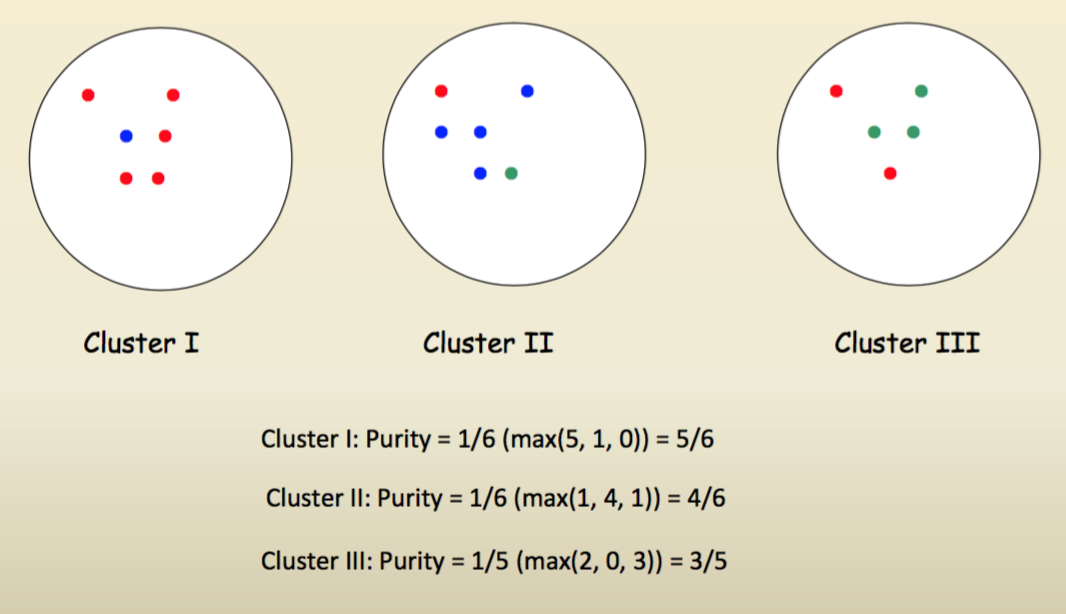
\includegraphics[width=\textwidth]{./notes/immagini/l17-purity.png}
\caption{Purity calcolata su 3 cluster}
\end{figure}

Nell'esempio il numero di cluster coincide con il numero di etichette ed è
una cosa voluta, ma il gioco funziona anche con un numero diverso di
cluster.

Questo perché le etichette note a priori vengono utilizzate solamente per valutare il clustering e non per effettuare l'apprendimento.

\subsubsection{Rand Index}\label{rand-index}

È una misura di similarità tra cluster, definita come il rapporto tra il
numero di elementi che hanno la stessa classe ground e si trovano nello
stesso cluster e con classi diverse in cluster diversi, sul numero
totale di elementi.

In altre parole è il rapporto tra il numero di elementi che si trovano nel cluster corretto e il numero totale di elementi.

\begin{figure}[htbp]
\centering
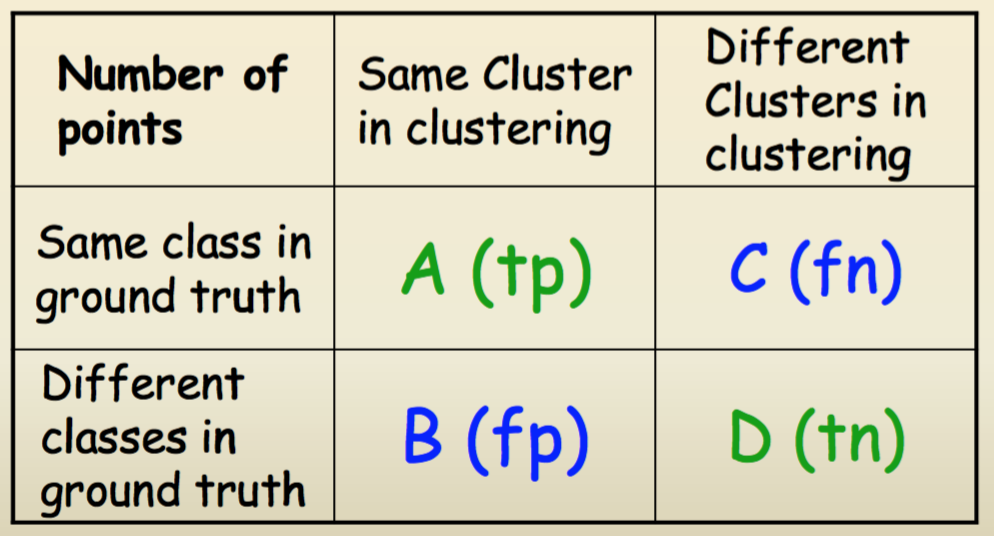
\includegraphics[width=0.6\textwidth]{./notes/immagini/l17-rand-index.png}
\caption{Elementi necessari per il Rand Index}
\end{figure}

Per calcolare il Rand Index, viene creata una tabella di contingenza, valutando per ogni coppia di
punti, se hanno etichette diverse e se sono nello stesso cluster.

Probabilmente, ma non ne sono sicuro, i numeri della tabella corrispondo
alle coppie che rispondo a quella categoria.

In questo modo ci si riconduce all'accuracy:

$$
RI =\frac{A + D}{A+B+C+D}
$$

Allo stesso modo si possono calcolare \textbf{precision} e
\textbf{recall} (§\ref{sec:pre-rec})

$$
P = \frac{A}{A+B} \qquad R = \frac{A}{A+C}
$$

\subsection{Algoritmi di Clustering}\label{algoritmi-di-clustering}

Ci sono due tipologie di algoritmi:

\begin{itemize}
\item
  \textbf{partitional}: che partono da un partizionamento casuale e
  cercano di migliorarlo iterativamente (K-means clustering, Model based
  clustering)
\item
  \textbf{hierarchical}: che vanno a definire un clustering come un
  albero in cui la radice contiene tutti gli esempi e man mano che si
  scende questi vengono partizionati. Si può usare un approccio
  \textbf{agglomerative} che costruisce l'albero in modo bottom-up
  (permettendo di fissare un numero di cluster), o \textbf{divisive} che
  funziona in top-down, applicando K-means sulla radice e poi
  ricorsivamente su ogni figlio, arrivando fino alla foglie che
  consistono in cluster di un solo elemento.
\end{itemize}

\subsection{K-means}\label{k-means}

Questo algoritmo appartiene alla categoria degli algoritmi di
partizionamento, ovvero vengono partizionati gli \emph{n} documenti in
\emph{K} cluster, cercando di trovare un partizionamento ottimo secondo
un determinato criterio.

Gli elementi da clusterizzare sono dei vettori con numeri reali e come
criterio di partizionamento si utilizza la distanza vettoriale tra gli
esempi e il centro del cluster.

Si cerca quindi di creare dei cluster che minimizzano il raggio della
iper-sfera che contiene gli esempi e che ha come centro $c$. (cluster \textbf{centroidi})

La formula da minimizzare è la seguente:

$$
\vec{\mu}(c) = \frac{1}{|c|}\sum_{\vec{x} \in c} \vec{x}
$$

\subsubsection{Algoritmo}\label{algoritmo}

\begin{enumerate}
\item
  Si posizionano K punti a caso nello spazio degli oggetti da
  clusterizzare, questi punti rappresentano i centroidi dei cluster.
\item
  Si assegna ogni oggetto al centroide più vicino.
\item
  Una volta completato l'assegnamento si ricalcola la posizione di tutti
  i centroidi utilizzano la media dei valori di tutti gli oggetti che
  sono finiti nel cluster.
\item
  Si ripetono i passi 2 e 3 finché non si spostano più i centrodi, ovvero finché non si raggiunge un punto fisso.
\end{enumerate}

L'iper-parametro $K$ dell'algoritmo è tipicamente soggetto a dei vincoli noti a priori oppure è da ottimizzare, ovvero trovare il numero \textit{corretto} di cluster in cui si dividono i dati.

\subsection{Approcci gerarchici agglomerativi}\label{approcci-gerarchici-agglormerativi}

\textbf{quelli divisi utilizzano ricorsivamente k-means}

Costruiscono un dendogramma a partire dagli oggetti, che vengono
agglomerati tra loro quando vengono trovati simili. Si ripete il
procedimento finché tutti gli oggetti non vengono agglomerati in un
unico cluster.

Si parte quindi da \textit{N} cluster, uno per ogni esempio e si agglomerano via
via finché non si ottiene un unico cluster.

Ad ogni iterazione l'algoritmo può essere interrotto per evitare di
ottenere un unico cluster.

Le linee verticale di un dendogramma rappresentano un cluster, mentre
quelle orizzontali rappresentano un punto di \textbf{merge} ovvero
quando la similarità di due cluster è tale che vengono uniti in un unico
cluster.

\begin{figure}[htbp]
\centering
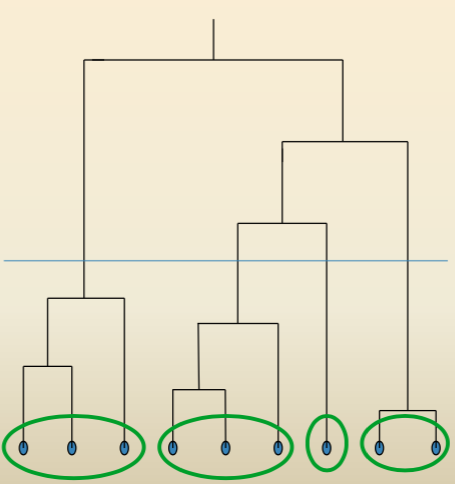
\includegraphics[width=.5\textwidth]{./notes/immagini/l17-clustering.png}
\caption{Esempio di un dendogramma}
\end{figure}

In base alla misura di similarità l'operazione può essere
\textbf{monotona} o meno, cioè se $s_1, \ldots, s_{k-1}$ sono
combinazioni di similarità associate a delle operazioni di merge, allora
$s_1 \geq s_2 \geq \ldots \geq s_{k-1}$

La non monotonicità, ovvero l'aumento della similarità in una serie di merge, contraddice l'assunzione fondamentale che cluster con pochi elementi sono più coerenti di cluster con tanti elementi\footnote{\url{http://nlp.stanford.edu/IR-book/html/htmledition/centroid-clustering-1.html}}.

\subsubsection{HAC - Hierarchical agglormerative
Clustering}\label{hac---hierarchical-agglormerative-clustering}

Prima viene creato un cluster per ogni esempio, dopodiché viene eseguito
via via il merge del \textbf{closest pair}, ovvero dei due cluster più
simili, fino a che non rimane un unico cluster. Lo storico dei merge
crea il dendogramma.

Come criteri di similarità tra i due cluster è possibile utilizzare:

\begin{itemize}
	\item la distanza euclidea: $||a-b||^2$, più è bassa, più simili sono i cluster
	\item la similarità coseno: $\frac{A \cdot B}{||A|| \cdot ||B||}$ che tende a 1 se i due esempi sono simili e a 0 se sono diversi.
	\item distanza di Manhattan: $\sum_i|a_i - b_i|$, più è bassa, più simili sono i cluster
\end{itemize}

Una volta scelta la misura di similarità, questa può essere calcolata per una coppia di cluster in vari modi:

\begin{itemize}
\item
  \textbf{single link}: viene calcolata la similiarità tra tutti gli elementi dei due cluster e viene scelto il valore massimo.
\item
  \textbf{complete link}: viene calcolata la similarità tra tutti gli elementi dei due cluster e viene scelto il valore minimo
\item
  \textbf{centroid link}: viene utilizzata la similarità tra i due centroidi dei due cluster
\item
  \textbf{average link}: viene calcolata la similarità tra tutti gli elementi dei due cluster e ne viene fatta la media.
\end{itemize}

Single, complete e average link garantiscono la monotonicità, mentre utilizzando centroid link alcune operazioni di merge potrebbero essere non monotone, ad esempio quando è necessario fare il merge di 3 cluster equidistanti tra loro.

Una volta calcolata la similarità tra tutti i cluster viene scelto il closest pair e viene fatto il merge.

\paragraph{Esempio - Distanza euclidea}

Scegliendo come misura la distanza euclidea, si ottiene che \textbf{minore è la distanza, più simili sono i cluster}. Pertanto i vari modi per calcolarle la similarità diventano:

\begin{itemize}
	\item
	\textbf{single link}: distanza tra i due punti più vicini dei due cluster
	\item
	\textbf{complete link}: distanza tra i due punti più lontani dei due cluster
	\item
	\textbf{centroid link}: distanza tra i centroidi dei due cluster
	\item
	\textbf{average link}: distanza media tra tutti i punti dei due cluster
\end{itemize}

\paragraph{Esempio - Similarità coseno}

Scegliendo come misura la similarità coseno, si ottiene che \textbf{maggiore è il valore, più simili sono i cluster}. Pertanto i vari modi per calcolarle la similarità diventano:

\begin{itemize}
	\item
	\textbf{single link}: similarità coseno tra i due punti più simili dei due cluster, ovvero che hanno similarità coseno più vicina ad 1.
	\item
	\textbf{complete link}: similarità cosento tra i due punti più diversi dei due cluster, ovvero che hanno similarità coseno più vicina a 0.
	\item
	\textbf{centroid link}: similarità coseno tra i due centroidi dei cluster
	\item
	\textbf{average link}: similarità media tra tutti gli elementi dei 
\end{itemize}

\begin{figure}[htbp]
\centering
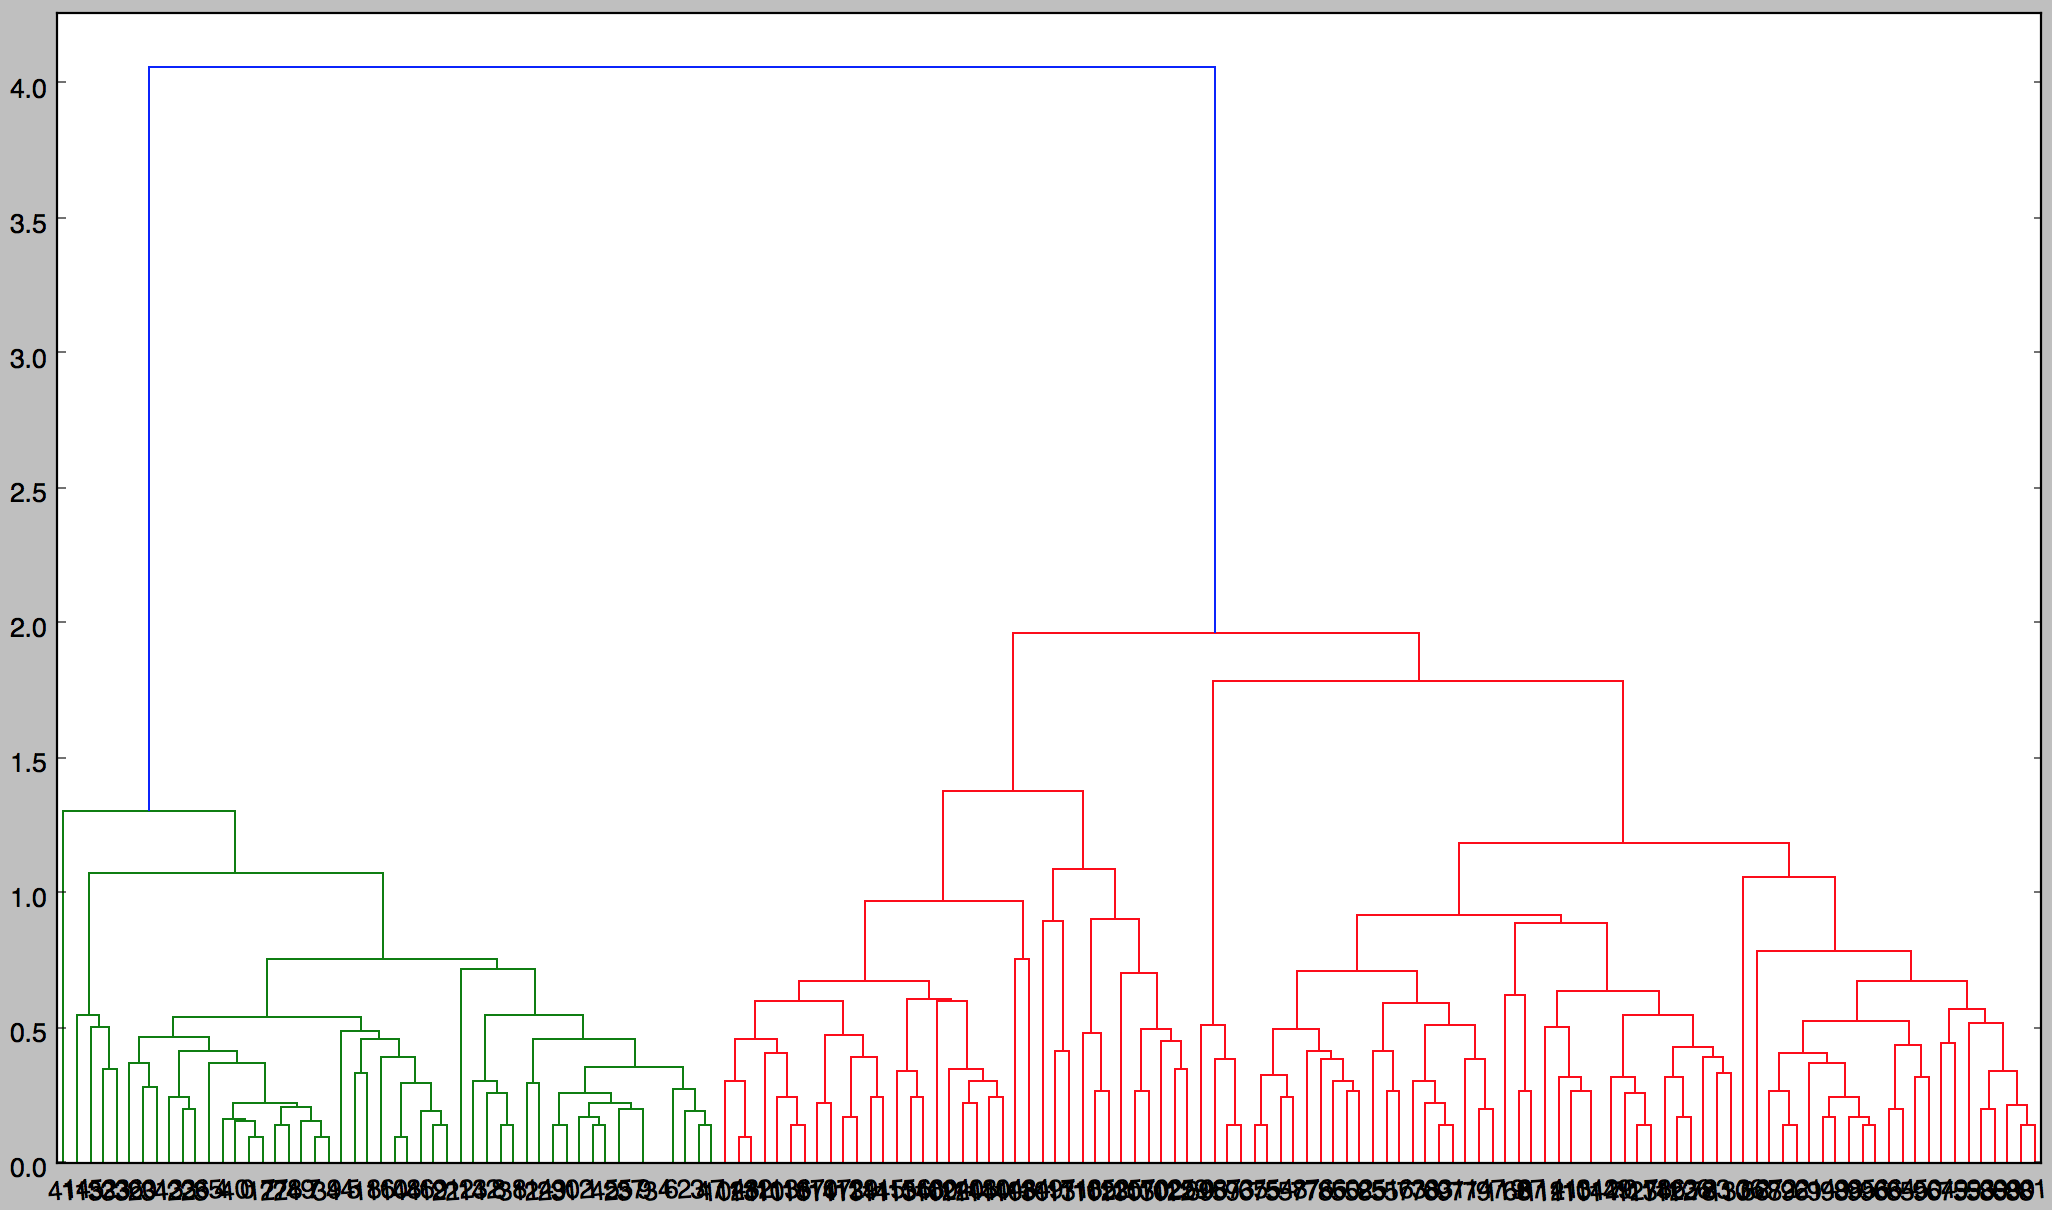
\includegraphics[width=\textwidth]{./notes/immagini/l17-dendogram-cluster.png}
\caption{Esempio di clustering ottenuto con HAC}
\end{figure}

Sia single link che complete link garantiscono la monotonia, tuttavia
con single link si tendono a creare dei cluster che sono delle
\emph{catene}, ovvero si ottengono dei dendogrammi sbilanciati, mentre
il complete link tende a dare dei cluster sferici e più compatti, se
però ci sono degli esempi \textbf{outliers}\todo{Da verificare}, ovvero che escono dalla
distribuzione.

Il centroid link è carino ma non garantisce la monotonia.

\begin{figure}[htbp]
\centering
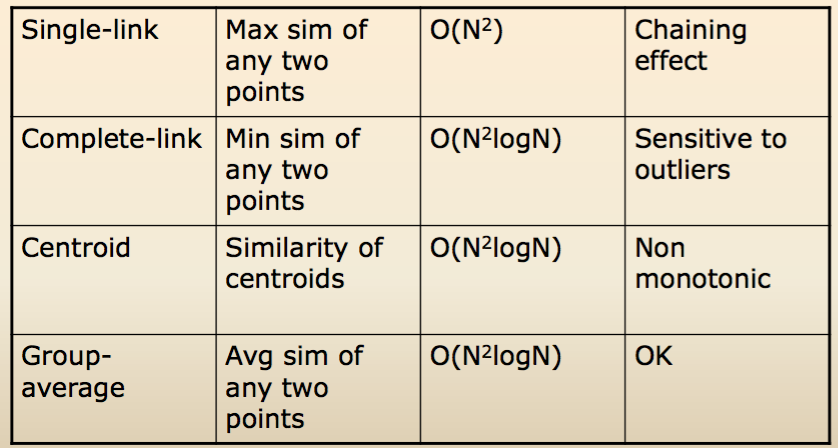
\includegraphics[width=\textwidth]{./notes/immagini/l17-riassunto.png}
\caption{Tabella riassuntiva, le complessità della tabella indicano quante operazioni servono per
	scegliere il closest pair}
\end{figure}

	% !TEX encoding = UTF-8
% !TEX TS-program = pdflatex
% !TEX root = computabilità e algoritmi.tex
% !TEX spellcheck = it-IT
\chapter{Programmi generici - Lezione 18}

\section{Enumerazione dei programmi}

\textbf{Enumerazione delle funzioni calcolabili}: Un insieme \textit{X} è numerabile se esiste una funzione $ f : \mathbb{N} \rightarrow X $ suriettiva tale che $ \underbrace{f(0), f(1), f(2), \ldots}_{\mathbb{N}} $.


\subsection{Enumerazioni di supporto}
Per poter enumerare e quindi codificare dei programmi è necessario prima definire alcune funzioni biunivoche di supporto:

\begin{enumerate}
	\item $ \Pi : \mathbb{N}^2 \rightarrow \mathbb{N}$
	\item $ \nu : \mathbb{N}^3 \rightarrow \mathbb{N}$
	\item $ \tau : \bigcup\limits_{k \geq 1}\mathbb{N}^k \rightarrow \mathbb{N}$
\end{enumerate}

\subsubsection{$1. \: \Pi $}

Già osservata precedentemente, ovvero è la codifica delle coppie:

\begin{align*}
\Pi(x, y) &= 2^x(2y + 1) - 1\\
\Pi^{-1}(n) &= (\Pi_1(n), \Pi_2(n))
\end{align*}

\subsubsection{$2. \: \nu $}

$\nu $ può essere definita utilizzando $ \Pi $:

\begin{align*}
\nu(x_1, x_2, x_3) &= \Pi(\Pi(x_1,x_2), x_3) \\
\nu'(n) &= (v_1(n), v_2(n), v_3(n)) \\
\nu_1(n) &= \Pi_1(Pi_1(n))
\end{align*}

\subsubsection{$3. \: \tau $}

$ \tau $ può essere definita come $ (x_1, \ldots, x_k) \rightsquigarrow \prod\limits_{i=1}^{k} P_{i}^{x_i} -1$ ma questa funzione non è iniettiva:

\begin{align*}
(2,1) &= 2^2 \cdot 3^1 -1 \\
(2,1,0) &= 2^2 \cdot 3^1  \cdot 5^0 -1
\end{align*}

pertanto è necessario utilizzare

$$
\tau(x_1, \ldots, x_k) \rightsquigarrow \prod\limits_{i=1}^{k-1} P_{i}^{x_i} \cdot P_{k}^{x_{k+1}} - 2
$$

Per decodificare un numero \textit{n} è necessario prima calcolare la lunghezza della decodifica:

$$
l(n) = \max k.P_k \text{ divide } (n+2) \text{ con } k \leq n
$$

Anche se si tratta di una massimizzazione illimitata è possibile dimostrare che è calcolabile sfruttando la minimalizzazione illimitata, e quindi $ l(n) \in \mathcal{PR} $.

$$
a(n,i) = \begin{cases}
(n+2)_i &\text{ se } i < l(n)\\
(n+2)_i -1 &\text{ se } i = l(n)
\end{cases}
$$

l'inversa di $ \tau $ può essere definita come:

$$
\tau^{-1}(n) = \Big(a\big(n,1\big), a\big(n,2\big), \ldots, a\big(n,l(n)\big)\Big)
$$

\subsection{Enumerazione dei programmi}

Grazie alle funzioni precedentemente definite è possibile definire delle codifiche biunivoche che permettono di codificare con un numero sia una singola istruzione URM, sia un qualsiasi programma URM in $ \mathcal{P} $.

$$
\beta : \text{Ist URM} \rightarrow \mathbb{N} \quad \text{e} \quad \gamma : \mathcal{P} \rightarrow \mathbb{N}
$$

\subsubsection{$ \beta : \text{Ist URM} \rightarrow \mathbb{N} $}

\begin{align*}
Z(n) &\rightarrow 4\cdot(n-1) \\
S(n) &\rightarrow 4\cdot(n-1)+1 \\ 
T(m,n) &\rightarrow 4\cdot\big(\Pi(m-1,n-1)\big)+2 \\
J(m,n,t) &\rightarrow 4\cdot\big(\tau(m-1,n-1,t-1)\big)+3
\end{align*}

I vari $ -1 $ servono perché i registri URM partono da 1, mentre la codifica deve partire da 0, altrimenti non sarebbe biunivoca.

La moltiplicazione per 4 serve per ``\textit{fare spazio}'' nella codifica in modo da continuare ad avere una funzione biunivoca. Allo stesso scopo servono anche le somme finali.

per fare l'inversa di $ \beta $ basta calcolare $ r = rm(4,n) $ e $ q = qt(4,n) $:

$$
\beta^{-1} \begin{cases}
Z(q+1) &\text{ se } r=0 \\
S(q+1) &\text{ se } r=1 \\
T\big(\Pi_1(q)+1, \Pi_2(q)+1\big) &\text{ se } r=2 \\
J\big(a(q,1)+1,a(q,2)+1,a(q,3)+1\big)&\text{ se } r=3
\end{cases}
$$
\todo{Verificare J}

In questo modo si ha una codifica per le istruzioni che permette di trasformare una sequenza di istruzioni in una sequenza di numeri

\subsubsection{$ \gamma : \mathcal{P} \rightarrow \mathbb{N} $}

$$
\gamma(P) = \tau\big(\beta(I_1), \beta(I_2), \ldots\big)
$$

inversa con:

$$
\gamma^{-1}(n) = \tau^{-1}(n) = \Big(a\big(n,1\big), a\big(n,2\big), \ldots, a\big(n,l(n)\big)\Big)
$$

\section{Verso il programma 33 e la sua funzione}

Con quanto a disposizione si può parlare del programma 33, ottenuto decodificando il numero 33.

Prima di continuare serve della notazione aggiuntiva:

Dato $ P \in \mathcal{P} $, $ \gamma(P) $ indica il codice di \textit{P} e prende il nome di \textbf{G\"odel number}.

Dato \textit{n}, $ \gamma^{-1}(n) $ rappresenta il programma codificato nel numero \textit{n}, tale programma viene indicato con $ P_n $.

Un esempio è dato da:
\begin{lstlisting}[language=URM]
P:
T(1,2) 		--> 4Pi(1-1, 2-1) +2= 10
S(2)		  --> 4(2-1) = 4
T(2,1)   	--> 4Pi(2-1,1-1) +2= 6
\end{lstlisting}

\begin{align*}
\gamma(P) &= \tau(10,4,6)\\
&= 2^10 + 3^4 + 5^{6+1} -2\\
&= 19.439.999.998
\end{align*}

\begin{lstlisting}[language=URM]
P':
S(1)		--> 2
\end{lstlisting}

$$
\gamma(P’) = \tau(P) = 2
$$

I numeri $ 19.439.999.998 $ e $ 2 $ rappresentano due programmi che calcolano la stessa funzione successore.

Si può fare anche l'operazione inversa:

\begin{verbatim}
100
gamma^{-1}(100)  100+2
= 2^1 + 3^1 + 17 ^1
P1^1 P2^1 P3^0 P4^0 P5^0 P6^0 P7^1
1 -> S(1)
1 -> S(1)
0 -> Z(1)
0 -> Z(1)
0 -> Z(1)
0 -> Z(1)
1 -> S(1)
\end{verbatim}

Il numero $ 100 $ rappresenta quindi il programma che calcola la constante 1.

Dal momento che è possibile codificare i programmi in un numero, viene indotta anche un'enumerazione sulle funzioni calcolate da questi programmi:

Fissata $ \gamma : \mathcal{P} \rightarrow \mathbb{N} $, si ha:

$$
\phi_{n}^{(k)} = f_{P_n}^{(k)}
$$

ovvero $ \phi_{n}^{(k)} $ è la funzione di \textit{k} argomenti calcolata da $ P_n = \gamma^{-1}(n) $.
Per questa funzione è possibile definire anche 

$$
W_{n}^{(k)} = dom(\phi_{n}^{(k)}) \subseteq \mathbb{N}^k = \{\vec{x}\: | \: \vec{x} \in \mathbb{N}^k \text{ tale che } \phi_{n}^{(k)}(\vec{x}) \downarrow\}
$$

$$
E_{n}^{(k)} = cod(\phi_{n}^{(k)}) = \{y\:|\: \exists\vec{x} \: \phi_{n}^{(k)}(\vec{x}) = y  \}
$$

Ad esempio:

\begin{align*}
P: S(1) &\rightarrow \gamma(P) = 2 \\
\phi_{2}^{(1)}(x) &= x+1 \\
W_{2}^{(1)} &= \mathbb{N} \\
E_{2}^{(1)} &= \mathbb{N} - \{0\} \\
\end{align*}

Inoltre, si può definire una sorta di funzione di ordine superiore che, una volta fissato un $ k \geq 1$, associa un numero $ \mathbb{N} $ ad una funzione in $ \mathcal{C}^{(k)} : n \rightarrow  \phi_{n}^{(k)}$. Questa funzione è suriettiva perché data $ f \in \mathcal{C}^{(k)} $ esiste un programma \textit{P} che calcola $ f = f_{P}^{(k)} = \phi_{\gamma(P)}^{(k)} $ .
Questa funzioni non è iniettiva perché una stessa funzione può essere calcolata da più programmi.

Quindi 

$$
|\: \mathcal{C}^{(k)}\:| =  |\: \mathbb{N}\:| \leq |\: \mathcal{C}\:| = |\: \bigcup\limits_{k \geq 1} \mathcal{C}^{(k)} \:| = |\: \mathbb{N}\: |
$$
\todo{Verificare}

ovvero esistono delle funzioni che non sono calcolabili.














	

\subsection{Miglioramento dell'efficienza con i Suffix Link}

Un primo miglioramento lo si ottiene utilizzando i \textbf{suffix link}, ovvero un collegamento tra due nodi espliciti dell'albero \textit{u} e $ s(u) $ tali che l'etichetta di $ u $ sia $ x\alpha $ e l'etichetta di $ s(u) $ sia $ \alpha $, in altre parole c'è un suffix link se l'etichetta di $ u $ è uguale all'etichetta di $ s(u) $ preceduta da un carattere qualsiasi (Fig \ref{asdasdasd2}).

\begin{figure}[htbp]
	\centering
	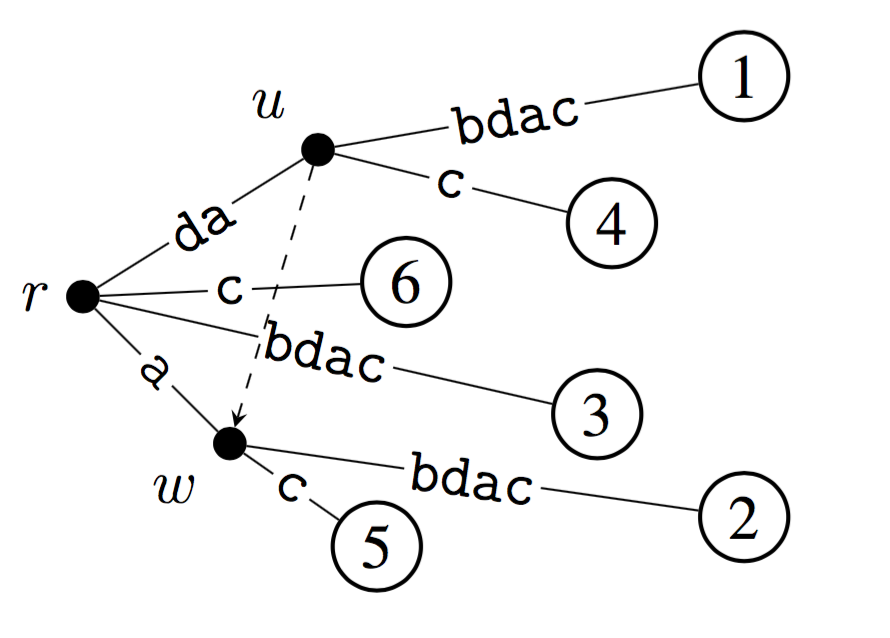
\includegraphics[width=.4\textwidth]{./notes/immagini/l22-fig1.png}
	\caption{In questo caso $\alpha=a$ e $x=d$}\label{asdasdasd2}
\end{figure}

Così facendo durante la costruzione dell'albero, quando viene esteso il cammino ad una foglia, posso tornare indietro fino a che non trovo un nodo esplicito con un suffix link e posso riprendere la costruzione dell'albero a partire dal nodo collegato.

Per ogni albero implicito $ I_i $, ogni nodo esplicito ha un suffix link uscente (\textbf{Lemma 5.4}), perché se durante la fase \textit{i}-esima per estendere il suffisso $ S[j,i] $, viene creato un nuovo nodo non foglia con etichetta $ x\alpha $ ($x\alpha$ prefisso di $ S[j,i] $) allora:

\begin{itemize}
	\item o nell'albero corrente esiste già un nodo interno esplicito con etichetta $\alpha$. Ad esempio perché la stringa $\alpha$ è un prefisso del suffisso $S[j+1, i-1]$ precedentemente inserito nell'albero.
	\item oppure tale nodo verrà creato immediatamente dopo con l'estensione del suffisso successivo $ S[j+1,i] $.
	
	Questo perché un nuovo nodo interno esplicito \textit{v} con etichetta $ S[j,i] = x\alpha $ viene creato soltanto se il suffisso $ S[j,i] $ viene esteso con il caso 2, quando nell'albero corrente il cammino $ S[j,i] $ termina in un nodo interno implicito e tale cammino continua con un carattere \textit{c} diverso da $S[i+1]$.
	Quindi nell'albero corrente c'è anche il cammino di etichetta $S[j+1,i] = \alpha$ che ha una continuazione che inizia con il carattere \textit{c}.
\end{itemize}

Dunque il nodo $ w $ con etichetta $ S[j+1, i]  = \alpha$ è un nodo interno che può essere esplicito o implicito. Se è esplicito $w = s(v)$ altrimenti, il cammino di etichetta $ S[j+1, i] = \alpha $ che termina nel nodo \textit{w} può continuare solo con \textit{c} e quindi nel passo successivo l'estensione del suffisso $ S[j+1,i] $ sostituisce il nodo implicito con un nodo esplicito per cui $s(v) = w$.

Inoltre (\textbf{Corollario 5.5}), nell'algoritmo di Ukkonen, ogni nodo interno esplicito creato durante l'estensione di un suffisso ha sicuramente un suffix link da esso uscente dopo che sia stato esteso anche un il suffisso successivo.

Questo si dimostra per induzione. Per $ I_0 $ la cosa è banalmente vera perché è presente solo un nodo interno esplicito e la radice non viene creata estendendo un suffisso.

Supponendo quindi che al termine della fase $(i-1)$-esima ci siano tutti i suffix link, per il lemma precedente, se viene creato un nuovo nodo \textit{v} estendendo $ S[j,i] $, il nodo $ s(v) $ viene trovato o creato durante l'estensione del suffisso successivo $ S[j+1,i] $. Siccome l'estensione dell'ultimo suffisso $ S[i+1,i] $ non aggiunge nodi interni, alla fine della fase $ i $-esima, tutti i nodi interni espliciti hanno il loro suffix link.

In altre parole, in ogni albero dei suffissi impliciti $ I_i $, se un nodo interno esplicito ha etichetta di cammino $ x\alpha $ esiste anche un nodo interno esplicito di etichetta $\alpha$.

\subsubsection{Costruzione dell'albero utilizzando i suffix link}

Nella fase di costruzione dell'albero $ I_{i+1} $ (fase $ i $-esima), l'algoritmo di Ukkonen cerca i nodi in cui terminano i suffissi $ S[j,i] $ per estenderli con il carattere $ S[i+1] $ (Nella fase $i$-esima viene esteso l'albero implicito $I_i$ per ottenere l'albero implicito $I_{i+1}$).

Il cammino relativo al suffisso $ S[1,i] $ sarà sempre presente e terminerà ogni volta in una foglia numerata, quindi questo può essere aggiornato sempre in tempo costante utilizzando il caso 1 e memorizzando un puntatore alla foglia.

Supponiamo di dover estendere un suffisso successivo $ S[j,i] $, uguale a quello precedente $ S[j-1,i] $ privato del primo carattere ($S[j-1,i] = x\alpha, S[j,i]= \alpha$, con $\alpha$ eventualmente nulla).

Sia \textit{v} l'ultimo nodo esplicito del cammino $ S[j-1,i] $, \textit{v} può essere la radice oppure un nodo interno di $ I_i $.

A questo punto, l'algoritmo per estendere il suffisso $ S[j,i] $ deve cercare nell'albero corrente il nodo con etichetta $ S[j,i] $.

Se \textit{v} è la radice, l'algoritmo si comporta come la versione ingenua e cerca il nodo a partire da essa.
Se invece \textit{v} è un nodo interno, per il corollario precedente, \textit{v} ha un suffix link $ s(v) $ e dato che l'etichetta di \textit{v} è un prefisso di $ x\alpha $, l'etichetta di $ s(v) $ è un prefisso di $\alpha$ e quindi per cercare il nodo con etichetta $ \alpha $ è possibile partire da $ s(v) $.

Più in dettaglio, l'estensione del suffisso $ S[j,i] $ avviene come segue:

\begin{enumerate}
	\item Sia $\beta$ l'etichetta del nodo $ s(v) $ e $ S[j,i] = \alpha = \beta\gamma $
	\item Per trovare la fine di $ S[j,i] = \alpha $ si parte da dove finisce $ S[j-1,i] = x\beta\gamma $ e si torna indietro al nodo \textit{v}.
	\item Si segue il suffix link per arrivare a $s(v)$ che ha $\beta$ come etichetta
	\item Si scende il cammino etichettato $\gamma$
	\item Alla fine di questo cammino c'è il nodo con etichetta $\alpha$, che può essere esteso con uno dei 3 casi.
\end{enumerate}

Come esempio vedi la figura \ref{sadefe2}

\begin{figure}[htbp]
	\centering
	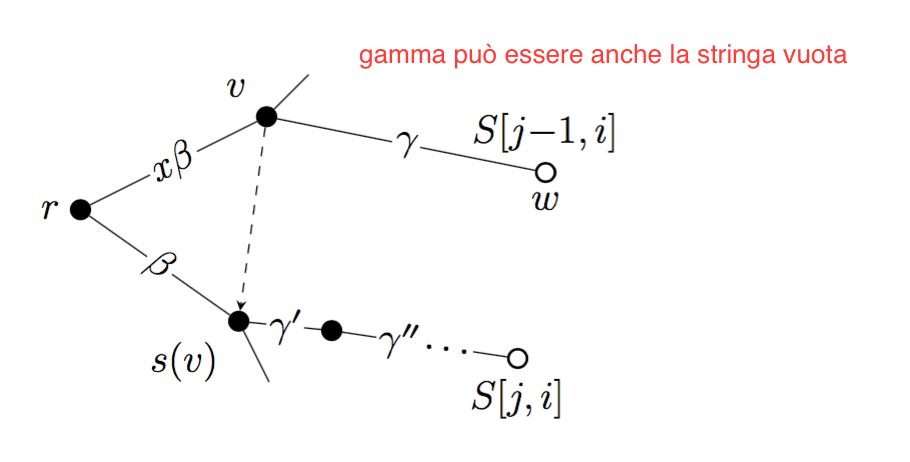
\includegraphics[width=.7\textwidth]{./notes/immagini/l22-fig3.png}
	\caption{La ricerca del suffisso $ S[j,i] $. Si risale, dal nodo con etichetta $ S[j-1,i] = x\alpha = x\beta\gamma $, per al più un arco $\gamma$ fino al nodo $ v $ di etichetta $ x\beta $; ci si muove quindi in $ s(v) $ utilizzando il suffix link e infine si scende il cammino cercando l'arco etichettato $\gamma = \gamma'\gamma''$ per arrivare al nodo di etichetta $ S[j,i] = \beta\gamma =\alpha$.}\label{sadefe2}
\end{figure}

Combinando il tutto l'algoritmo per l'estensione di un suffisso diventa:

\begin{enumerate}
	\item Partendo dal nodo $ w $ dove termina il suffisso $ S[j,i] $ e risalendo verso la radice, cerca il primo nodo esplicito \textit{v} che o ha un suffix link oppure è la radice. Per i corollari precedenti richiede di risalire al massimo di un solo arco.
	
	Sia $\gamma$ l'etichetta, eventualmente nulla, del cammino dal nodo \textit{v} al nodo \textit{w}.
	
	\item Se \textit{v} non è la radice spostati su  $s(v)$ usando il suffix link e quindi discendi seguendo il cammino individuato dalla stringa $ \gamma $.
	
	Se \textit{v} è la radice segui il cammino individuato dalla stringa $ S[j+1,i] $ come per l'algoritmo ingenuo.
	
	\item Estendi il suffisso $ S[j+1,i] $ usando il caso appropriato.
	
	\item Se il nodo \textit{w} è un nodo interno esplicito creato durante l'estensione del suffisso precedente $S[j,i]$ (usando il caso 2), per il lemma 5.4 la stringa $ S[j+1,i] $ deve terminare in un nodo $ s(w) $ esplicito dopo l'estensione di $ S[j+1,i] $. In questo caso metti un suffix link da $ w $ a $ s(w) $
\end{enumerate}

Inoltre, mantenendo un puntatore alla foglia relativa al suffisso più lungo $ S=[1,i] $, la prima estensione della fase \textit{i}-esima non richiede alcuna ricerca e può essere fatta direttamente con il caso 1.

Nonostante ciò la complessità asintotica nel caso pessimo, con una stringa composta da tutti caratteri diversi, non migliora e risulta essere $ O(n^3) $.

\subsubsection{Skip - count}

Durante il secondo passo l'algoritmo discende dal nodo $s(v)$ al cammino di etichetta $\gamma$ e se questo viene fatto normalmente richiede un tempo proporzionale alla lunghezza di $\gamma$.

Sia $g = |\gamma|$ la lunghezza della stringa $\gamma$. Sappiamo che esiste un cammino etichettato con $\gamma$, che può essere anche nullo.

Se $g = 0$, il nodo $s(v)$ è proprio il nodo d'interesse, altrimenti, siccome tutti gli archi uscenti da $s(v)$ hanno etichette che iniziano con caratteri distinti, la scelta dell'arco lungo cui scendere richiede soltanto il confronto con il primo carattere di $\gamma$.

Sia $b$ la lunghezza dell'arco $\beta$ prescelto, tale lunghezza può essere memorizzata assieme all'etichetta.

\begin{itemize}
\item Se $b \leq g$ l'algoritmo non deve controllare nessun altro carattere di $\beta$, perché $\beta$ è certamente uguale al prefisso di $\gamma$ di lunghezza $b$, ossia $\gamma = \beta\gamma'$. L'algoritmo si sposta quindi direttamente sul nodo finale dell'arco prescelto per continuare la ricerca del cammino etichettato $\gamma'$.
\item Se $b > g$ il cammino etichettato $\gamma$ termina nel nodo implicito $g$-esimo di tale arco.
\end{itemize}

Assumendo quindi costante la dimensione dell'alfabeto, ogni spostamento da un nodo esplicito ad un altro nodo lungo il cammino etichettato $\gamma$ richiede un tempo costante.

Il \textbf{livello} $l(v)$ di un nodo esplicito \textit{v} è definito come il numero di archi del cammino dalla radice a \textit{v} o, equivalentemente, come il numero di nodi espliciti che precedono \textit{v} in tale cammino.

Si ha quindi che durante l'esecuzione dell'algoritmo di Ukkonen, viene attraversato un suffix link da $v$ a $s(v)$, vale il \textbf{Lemma 5.7}:

$$
l\big(s(v)\big) \geq l\big(v\big) -1
$$

Questo perché ogni nodo esplicito che precede \textit{v}, esclusa la radice, ha un suffix link che punta ad un nodo che precede $s(v)$. Infatti se l'etichetta del cammino di $v$ è $x\beta$, prefisso del suffisso precedente $S[j,i]$, l'etichetta di cammino di $s(v)$ è $\beta$, prefisso del suffisso $S[j+1,i]$.

Usando quindi lo skip/count, ogni fase dell'algoritmo di Ukkonen richiede tempo $O(n)$.

Infatti, nella fase $i$-esima vengono effettuate $i+1$ estensioni. In ogni estensione l'algoritmo risale al più di un solo arco per trovare il nodo con suffix link, attraversa il suffix link, discende un certo numero di archi e quindi applica uno dei tre casi per l'estensione del suffisso ed eventualmente aggiunge un suffix link. Tutte queste operazioni possono essere fatte in tempo costante, tranne la discesa che dipende dal numero di archi percorsi.

Consideriamo come varia il livello corrente $l$ durante una fase, ossia il livello dell'ultimo nodo esplicito visitato dall'algoritmo.
L'estensione del primo suffisso non modifica $l$ perché applica il caso 1 sul suffisso più lungo.

Ad ogni estensione successiva, \textit{l} diminuisce al più di una unità nella risalita, diminuisce al più di una unità attraversando il suffix link ed aumenta di una unità ogni volta che si discende un arco. Quindi durante l'intera fase \textit{l} può diminuire al più $2i$ volte.

Siccome $l$ rimane sempre $\leq i$, ogni arco ha un'etichetta di almeno un carattere e le etichette sono lunghe al massimo $i$), esso non può aumentare più di $3i$ volte e quindi il numero totale di archi discesi in tutta la fase è al più $3i = O(n)$.

Ricapitolando:
\begin{itemize}
	\item Estendere un suffisso con uno dei 3 casi viene fatto in tempo costante, l'importante è trovare cammino dell'albero da estendere
	\item Utilizzando il suffix-link e lo skip/count ogni fase, l'estensione dell'albero dei suffissi $I_i$ per la stringa $S[1,i]$ nell'albero dei suffissi $I_{i+1}$ per la stringa $S[1,i+1]$, può essere fatta in $O(n)$, questo perché entrambi gli accorgimenti velocizzano la ricerca dei cammini e il numero di archi discesi durante la fase è al massimo $3i = O(n)$.
	\item Per ottenere l'albero dei suffissi per la stringa sono necessarie $n$ fasi.
\end{itemize}

In tutto si ha una complessità di $O(n^2)$.

\subsubsection{Il problema dello spazio}

Al momento l'albero dei suffissi può richiedere uno spazio $O(n^2)$ e ovviamente non può essere costruito in $O(n)$.

Questa occupazione in spazio deriva dal fatto che, anche se i nodi dell'albero non possono essere più di $2n-1$, la somma delle lunghezze delle etichette può richiedere $O(n^2)$. I nodi dell'albero sono le $n$ foglie ed al più $n-1$ nodi interni (perché ogni nodo ha almeno due figli). Nel caso di una stringa con tutti i caratteri distinti, l'albero dei suffissi è costituito soltanto dalla radice e dalle $n$ foglie e la somma delle lunghezze delle etichette è $\sum_{i=1}^n i = O(n^2)$.

La soluzione è quindi quella di rappresentare l'etichetta di un arco con una coppia di indici $(p,q)$ tale che l'etichetta sia $\beta = S[p,q]$, resta inoltre possibile calcolare la lunghezza per effettuare lo skip count con $b = q -p+1$.

Utilizzando le coppie di indici lo spazio richiesto per memorizzare un'etichetta diventa costante.

\subsubsection{Limitazione delle fasi}

Si può osservare che non appena in una fase viene applicato il caso 3, questo viene applicato anche a tutte le successive estensioni della stessa fase.

Questo perché, se viene applicato il caso 3 per l'estensione del suffisso $S[j,i]$ significa che il suffisso $S[j,i+1]$ è già presente nell'albero corrente e quindi sono presenti anche tutti i suffissi successivi da $S[j+1,i+1]$ ad $S[i+1,i+1]$.
Ovvero quando viene applicato il caso 3 vuol dire che all'interno dell'albero è già stato inserito il suffisso $S[j',i+1]$ che ha come prefisso $S[j,i+1]$ per $j' < j$.

Si ha quindi che non appena viene applicato il caso 3, la fase di estensione dell'albero può terminare.

Inoltre, se ad un certo punto dell'algoritmo di Ukkonen viene creata una foglia etichettata \textit{j} per inserire il suffisso $S[j,i+1]$ (caso 2) tale foglia rimane una foglia in tutti i successivi alberi costruiti dall'algoritmo, questo perché l'algoritmo non estende mai un cammino oltre la foglia che lo termina. Quindi tutte le estensioni successive del suffisso associato a tale foglia verranno sempre fatte applicando il caso 1.

L'esecuzione di una fase dell'algoritmo quindi procede sempre secondo un determinato schema:

\begin{enumerate}
	\item La foglia 1 viene costruita nella fase 1, quindi ogni fase inizia con un'estensione che usa il caso 1.
	\item Vengono poi eseguite delle estensioni che usano i casi 1 e 2
	\item Termina non appena viene eseguito il primo caso 3.
\end{enumerate}

Sia $j_{i-1}$ l'ultima estensione che usa i casi 1 o 2 nella fase $(i-1)$-esima. Siccome ogni applicazione del caso 2 crea una nuova foglia, alle prime $j_{i-1}$ estensione della fase successiva si applica il caso 1, per quanto precedentemente osservato.

Dunque per la fase successiva si avrà $j_i \geq j_{i-1}$ e questo ci suggerisce di cercare un trucco che faccia evitare, nella fase successiva, le prime $j_{i-1}$ estensioni che utilizzano il caso 1.

Si può osservare che il caso 1 si limita ad aggiungere all'etichetta dell'arco che termina nella foglia di etichetta $S[j,i]$ il carattere $S[i+1]$.
Quando viene creata una foglia con il caso 2 nella fase $i$-esima all'arco che termina nella foglia viene assegnato solamente il carattere $S[i+1]$ come etichetta. 
Da quel momento in poi l'etichetta verrà via via allungata di un carattere per ogni fase, fino a diventare $S[i+1,n]$.

Si può quindi assegnare, alla creazione della foglia come caso 2, l'etichetta $S[i+1,n]$, sempre se la stringa è nota a priori. Se questo non lo è come coppia che identifica l'etichetta è possibile utilizzare il valore $(i+1,e)$.

Così facendo le prime $j_{i-1}$ estensioni nella fase $i$-esima, non richiedono alcuna operazione e possono essere saltate, iniziando all'estensione $(j_{i-1}+1)$-esima. La fase $i$-esima inizia quindi con l'estensione $j = i_{j-1}+1$ e termina con la prima estensione che usa il caso 3 oppure quando tutti i suffissi sono stati estesi (in questo caso si ha $j = i+2$).

Il valore per la fase successiva risulta essere $j_i = j-1$, ovvero l'ultima posizione che non è stata estesa con il caso 3.

\begin{figure}[htbp]
	\centering
	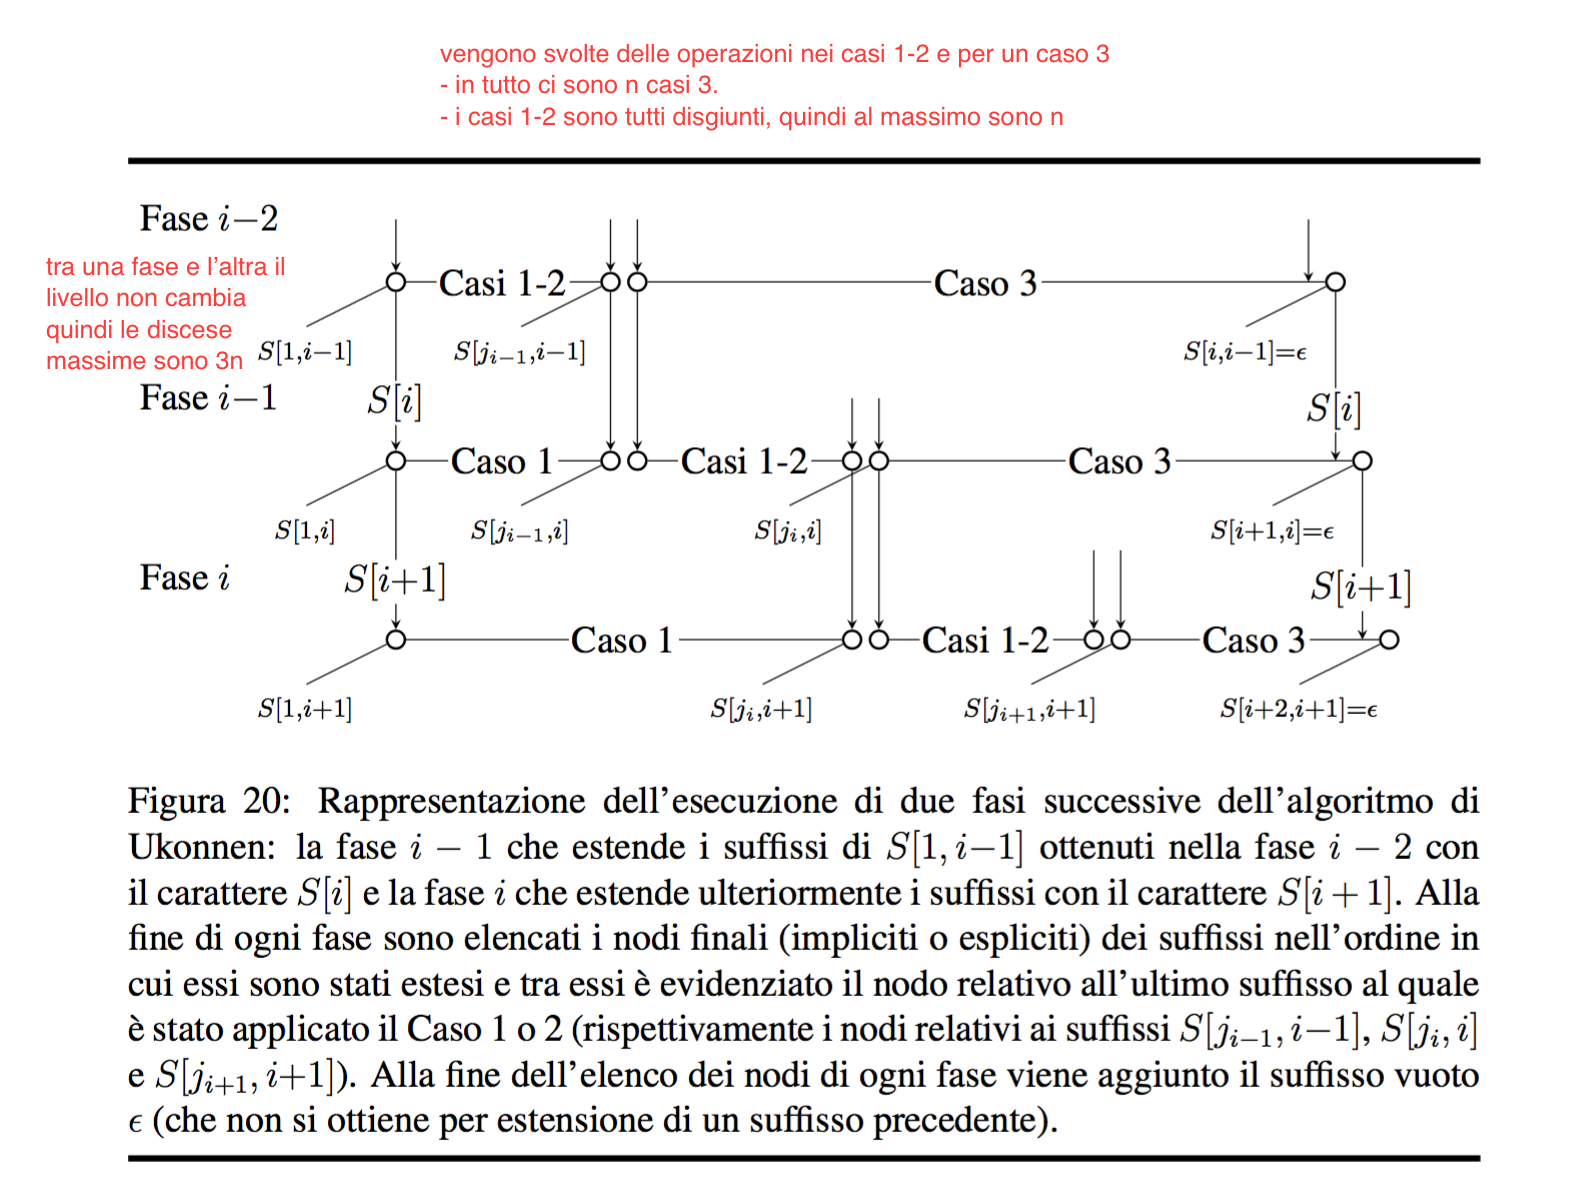
\includegraphics[width=.9\textwidth]{./notes/immagini/l22-fig8.png}
\end{figure}

\paragraph{Dimostrazione del tempo di esecuzione costante}

Se $S[j*, i-1]$ è l'ultimo suffisso esteso nella fase $(i-1)$-esima, la fase $i$-esima inizia con l'estensione del suffisso $S[j*,i]$. Dunque soltanto il suffisso $j*$-esimo viene esteso sia nella fase $(i-1)$-esima che nella fase $i$-esima.

Siccome gli indici $j$ dei suffissi sono tutti minori o uguali ad $n$ e le fasi sono $n$, in totale vengono eseguite al più $2n$ estensioni durante tutta l'esecuzione dell'algoritmo, con ogni estensione che richiede un tempo costante più un tempo proporzionale al numero di archi discesi nella ricerca di $\gamma$, che è un $O(n)$.

Siccome la fase $i$-esima inizia con il suffisso $j*$-esimo in cui è avvenuta l'ultima estensione della fase precedente, il livello corrente non cambia passando da una fase alla successiva (anche nel caso in cui $j_{i-1}=i$, il livello corrente quando si è esteso l'ultimo suffisso $S[i,i-1] = \epsilon$ nella fase $(i-1)$-esima era 0, uguale al livello corrente quando si estende il primo suffisso $S[i+1,i] = \epsilon$ nella fase $i$-esima).

Dunque il fatto che il livello corrente non diminuisca mai più di due volte vale sia all'interno di una singola fase che per tutto l'algoritmo e siccome il livello rimane sempre compreso tra 0 e $n$, il numero di archi discesi durante tutta l'esecuzione dell'algoritmo deve essere minore o uguale a $3n$.

Questo perché nella stessa fase, per quanto precedentemente dimostrato, il livello diminuisce al più di due volte e tra una fase e l'altra il livello non cambia.

Siccome durante tutta l'esecuzione dell'algoritmo vengono eseguite al più $2n$ estensioni ciascuna delle quali richiede un tempo costante più un tempo proporzionale agli archi discesi e il numero totale di archi discesi è minore o uguale a $3n$ si può concludere che l'algoritmo richiede un tempo $O(n)$. Questo perché nelle $2n$ estensioni vengono discesi al massimo $3n$ archi, si ha quindi come complessità $O(2n)+ O(3n) = O(n)$.

Se la lunghezza della stringa non è nota a priori, una volta completata l'esecuzione è necessario andare a correggere le etichette delle foglie.

L'algoritmo di Ukkonen quindi, costruisce on-line l'albero dei suffissi di una stringa di lunghezza $n$ in $O(n)$.
	% !TEX encoding = UTF-8
% !TEX program = pdflatex
% !TEX root = InformationRetrieval.tex
% !TEX spellcheck = it-IT

\section{Search Engine Optimization}

Il linguaggio HTML non è stato pensato per i motori di ricerca e per farci reperimento dell'informazione. Tutto è iniziato per trovare un modo di rappresentare dei documenti che funzionasse anche per non informatici.

\subsection{Ranking delle pagine}

Il \textbf{ranking statico} viene definito nel momento dell'indicizzazione effettuando l'analisi del contenuto e dei link presenti nella pagina web.

Questo dipende dall'uso dei link e dalla struttura della pagina, la quale deve riflettere la qualità, l'autorevolezza e la popolarità di una pagina web. 
Migliore è la qualità della pagina, maggiore è il rank statico calcolato dal motore per la pagina.

Da notare che se un motore di ricerca fornisce tra i primi risultati una pagina autorevole non implica che è un motore che funziona bene.

Il \textbf{ranking dinamico} viene calcolato combinando la query con il ranking statico delle pagine. Vengono quindi presi in considerazione alcuni fattori che dipendono dalla query come la presenza dei termini e le loro prossimità.
Le modalità di ranking statico e dinamico variano da motore a motore.
Tuttavia, anche se ci sono vari algoritmi, ci sono due comportamenti tipici:

\begin{itemize}
	\item \textbf{Testo delle ancore}: l’efficacia del reperimento può essere aumentata sfruttando il testo delle ancore
	\item \textbf{Novità} o \textbf{Novelty}: piuttosto che restituire tante pagine di uno stesso sito, viene fornita solo quella principale. In modo da fornire dei risultati che sono il più vari possibili.
\end{itemize}

\subsection{SEO}

L'idea è quella di aumentare il ranking delle pagine in modo che il proprio sito finisca tra i primi risultati del motore di ricerca.
Infatti, un buon posizionamento permette una maggiore visibilità e sperabilmente aumenta il traffico in entrata del sito.
Ovviamente un prerequisito fondamentale è quello che la pagina web sia indicizzata dai principali motori di ricerca.

Tipicamente gli aspetti SEO sono strettamente legati alla qualità del sito web. Maggiore è la qualità, maggiore è la probabilità che il sito sia ben posizionato in una ranking list.

La qualità del sito dipende:

\begin{itemize}
	\item dai contenuti che devono essere buoni e scritti correttamente.
	\item dalla frequenza di aggiornamento del sito, che deve essere specificata sia nei meta-tag, che sotto forma di data presente negli articoli.
	\item dalla manutenzione della pagina. \`E strettamente legato all'aggiornamento.
	\item dal codice, che deve essere pulito e ben formato. Non devono essere presenti parti di codice ridondanti e il codice deve essere scritta con una sintassi corretta.
	\item dall'autorevolezza della pagina, la quale dipende dai link che ci sono in entrata verso il sito.
\end{itemize}

Ovviamente essere visti da un motore di ricerca permette di essere visti da molte persone e quindi produce valore per le attività commerciali.

Da notare che \textbf{nessuna} pratica di SEO ha un'efficacia garantita.
Questo perché tutte le tecniche di SEO sfruttano un approccio empirico che interpreta in modo approssimato il comportamento dei motori di ricerca e cerca di mettere in atto delle azioni che possano essere utilizzate opportunamente da questi.

Quindi noi possiamo solamente cercare di migliorare il sito e i suoi contenuti, nella speranza che i motori di ricerca ci ritengano autorevoli, senza nessuna certezza, questo perché i motori di ricerca utilizzano molti criteri per stabilire il rank di una pagina.

Alcune caratteristiche che vengono giudicate positivamente dai motori di ricerca sono:

\begin{itemize}
	\item Presenza di uno o più termini della query nel tag \texttt{<title>} della pagina.
	\item Presenza di un termine della query nel \texttt{<body>}.
	\item Utilizzo del tag \texttt{<strong>} attorno ad un termine della query.
	\item Presenza di un termine di ricerca in un elemento \texttt{<heading>} o \texttt{<a>}. Un ancora in uscita con un termine della query viene ben vista, perché il ragionamento è quello del ``\textit{l'autore non manderebbe mai via l'utente dal suo sito se l'informazione non è molto importante, quindi il contenuto della pagina che contiene l'ancora deve essere ben fatto}''.
	\item Autorevolezza dei link che puntano verso la nostra pagina. Può essere determinata utilizzando delle liste di domini ritenuti autorevoli.
	\item Velocità di caricamento del tipo. Ad esempio, le immagini devono essere delle dimensione corrette, in modo che il loro caricamento sia veloce. Lo stesso vale per tutti gli altri file multimediali.
\end{itemize}

Queste caratteristiche sono state derivate dallo studio della letteratura, anche se limitata, e da prove pratiche.

Altri aspetti che invece vengono considerati negativamente sono:

\begin{itemize}
	\item La presenza dei trattini (hypens) nell'URL. Non si sa bene il perché.
	\item Lunghezza dell'URL. Se l'URL è lungo, vuol dire che si sta andando in profondità del sito e quindi il contenuto è stato messo in disparte, appunto perché è in profondità.
	\item Lunghezza del tag \texttt{<title>}, non deve essere né troppo lungo, né troppo corto.
	\item Quantità di pubblicità presente nella pagina. Se ce n'è troppa la pagina viene penalizzata.
	\item Numero di immagini e video. Non solo la pesantezza, ma anche lo spazio che occupano sullo schermo.
\end{itemize}

Ci sono poi altri aspetti che influenzano il ranking. Questi si dividono in due categorie:

\begin{itemize}
	\item \textbf{On the page}: sono quelli sotto il controllo dell'autore della pagina, come il contenuto, la struttura HTML e l'architettura del sito.
	\item \textbf{Off the page}: sono fattori esterni non direttamente controllabili, come la qualità dei link che puntano al nostro sito, l'autorevolezza dei contenuti e la reputazione social.
\end{itemize}

\subsubsection{On the page}

Uno dei fattori più importanti è il contenuto della pagina, il quale deve essere originale. 
I contenuti copiati, in parte o del tutto, influiscono negativamente sul ranking e contribuiscono a far diminuire l'autorevolezza e la credibilità di un sito. Il contenuto dovrebbe essere \textbf{unico}, \textbf{diverso} e \textbf{utile}.

\begin{figure}[htbp]
	\centering
	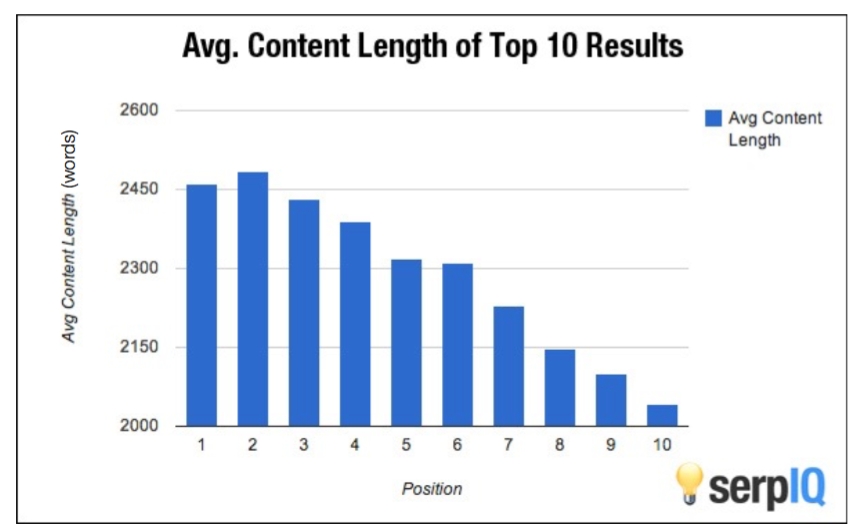
\includegraphics[width = 0.5\textwidth]{images/l23-fig-1}
	\caption{Contenuti lunghi e approfonditi sono in genere preferiti}
\end{figure}

Alcuni motori di ricerca calcolano il livello di leggibilità dei siti web, dove un alto livello di leggibilità (basso valore per il motore) indica un sito con contenuti ``\textit{facili e adatti alle masse}'' mentre un basso livello di leggibilità indica ``\textit{contenuti più complessi e elitari}''.
Non è chiaro cosa sia preferibile, ma il ranking può essere categorizzato in base a questo indice.

Anche la presenza \textbf{parole chiave} relative all'argomento del sito all'interno del contenuto è importante.

\paragraph{Title} Il tag \texttt{<title>} gioca un ruolo molto importante, sia a livello di ranking, sia perché viene mostrato tra i risultati della ricerca che vengono forniti all'utente.
\`E quindi buona norma utilizzare dei titoli correlati all'argomento della pagina, che contengano delle parole chiavi e non troppo lunghi. All'interno del titolo può anche comparire il brand del sito.

\paragraph{Meta-tag}Anche i meta-tag della sezione \texttt{head} sono molto utilizzati dai motori di ricerca e vengono utilizzati per popolare gli snippet presenti nella pagina dei risultati.
Non c'è la certezza, ma sembra che vengano apprezzati dai motori di ricerca.

\paragraph{Dimensione e immagini} La dimensione in byte della pagina gioca un ruolo fondamentale, perché viene presa sia in considerazione dai motori di ricerca che dagli utenti del sito, è quindi importante che ci sia un equilibrio tra testo e immagini.
La presenza delle immagini deve essere anche limitata perché i crawler raccolgono solo una parte della pagina, e se la parte della pagina comprende tante immagini, queste non forniscono informazioni utili.
\`E inoltre sconsigliato utilizzare delle immagini come testi per i link.

\paragraph{Struttura della pagina} I crawler preferiscono le pagine poco profonde, con una struttura semplice perché risultano più semplici da indicizzare. \`E quindi sconsigliato utilizzare le tabelle HTML ed è incentivato l'uso dei \texttt{<div>} opportunamente stilati con i CSS.
Tutto lo stile della pagina dovrebbe essere contenuto in un file CSS seprato, sia per una questione di separazione della presentazione dal contenuto, sia perché questo alleggerisce le dimensioni della pagina.
\`E inoltre importante prestare attenzione alla \textbf{site crawlability} della pagina, ovvero i contenuti dovrebbero essere facilmente accessibili dal crawler, quindi attenzione al JavaScript che potrebbe nascondere delle informazioni e niente Adobe Flash.
Sempre per facilitare il lavoro del crawler è utile specificare nel file \texttt{robot.txt} quali pagine non indicizzare, questo perché il tempo del crawler sul sito è limitato ed è meglio che eviti di sprecarlo su pagine inutili. L'utilizzo di una sitemap può agevolare ulteriormente il crawler.

\paragraph{Contesto} Il contesto geografico, temporale, sociale in cui viene effettuata una ricerca viene preso in considerazione dai motori di ricerca. Quindi possono influire positivamente sul ranking i seguenti fattori:

\begin{itemize}
	\item Indicare la città o lo stato nel tag \texttt{<title>}
	\item Il fatto che la regione del dominio o l'indirizzo fisico del server coincida con la regione in cui è stata effettuata la ricerca.
	\item Presenza della città o stato nei tag di heading.
\end{itemize}

\subsubsection{Off the page}

Anche i social network influiscono sul ranking di una pagina, infatti se una pagina viene spesso condivisa, twittata, riceve like ed è attiva sui social, il suo ranking aumenta.

L'altro fattore off the page che influisce principalmente sul ranking è l'autorevolezza del sito, determinata dai contenuti, dalla reputazione dell'autore e dallo storico del dominio. Domini più vecchi sono preferiti in quanto sono resistiti nel tempo.


\subsubsection{Riferimenti utili}

\begin{itemize}
	\item \url{http://searchengineland.com/}
	\item \url{http://moz.com/search-ranking-factors/}
\end{itemize}









	% !TEX encoding = UTF-8
% !TEX program = pdflatex
% !TEX root = InformationRetrieval.tex
% !TEX spellcheck = it-IT

% 15 Dicembre 2016

\chapter{Anatomia e performance di un sistema di IR}

Nel nostro progetto noi non stiamo misurando lo stemmer di per se, ma stiamo misurando quanto lo stemmer migliora i risultati del sistema rispetto all'esecuzione senza stemming.

Si ha però che il sistema è composto da molti blocchi: tokenizzatore, stoplist, stemmer, modello e quindi non è semplice valutare il singolo componente, perché le prestazioni del sistema possono essere influenzate dagli altri componenti o dai parametri con i quali sono configurati.

Le misure nell'IR sono quindi misure end-to-end che considerano la totalità del sistema. Per valutare un singolo componente stabilisco quindi una pipeline di componenti e vario solamente quello che voglio misurare.

\section{Grid@CLEF}

L'idea è quindi quella di sviluppare un sistema di testing che funzioni con più lingue (MLIA: Multilingual Information Access) per capire come migliorare le performance dei singoli componenti.

Questo si può ottenere conducendo una serie di griglie di esperimenti, sistematici e ripetibili, su diversi linguaggi e con diversi componenti, effettuando uno sforzo comunitario per valutare sia i singoli componenti che la loro interazione con gli altri.

Per implementare questo sistema è stata sviluppata una soluzione asincrona, basata su una produzione di dump intermedi XML, da scambiare tra i vari gruppi di ricerca. Ad esempio quelli che lavoro su un tokenizzatore, possono fornire i loro output ad un gruppo di ricerca che lavora agli stemmer per il tedesco.
Ci sono stati dei problemi implementativi però qualcosa si è riuscito a fare.

\begin{figure}[htbp]
	\centering
	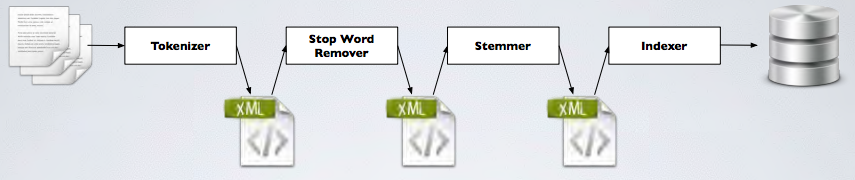
\includegraphics[width=0.5\textwidth]{images/l20-fig-1}
	\caption{Utilizzo dei file XML condivisi dai vari gruppi di ricerca.}
\end{figure} 

Mancava però una metodologia per analizzare i risultati di questi esperimenti.

Nel 2015 alla conferenza SIGIR-RIGOR si è iniziato ad invitare gli sviluppatori di motori open-source a fornire delle baseline di valutazione per i loro sistemi in un ambiente comune.
L'idea era quella di creare questo ambiente comune dove chi volesse valutare una nuova tecnica fosse in grado di utilizzare un motore di ricerca già esistente per il confronto/implementazione. Questo ambiente doveva essere anche aperto in modo che fosse possibile capire se durante i test i sistemi utilizzati fossero stati configurati nella maniera corretta.
Si voleva quindi fornire una baseline da utilizzare come riferimento per i nuovi metodi e allo stesso modo la baseline era in un certo senso certificata perché era nota a tutti e quindi se qualcuno ha presentato dei nuovi modelli comparandoli con una baseline è possibile capire se la baseline di riferimento è sufficientemente buona e quindi i risultati sono concreti, oppure se è stata scelta una baseline pessima e quindi i risultati sembrano migliori di quanto lo sono in realtà.

Ma anche in questo caso mancava una sistema di analisi dei dati.

\begin{figure}[htbp]
	\centering
	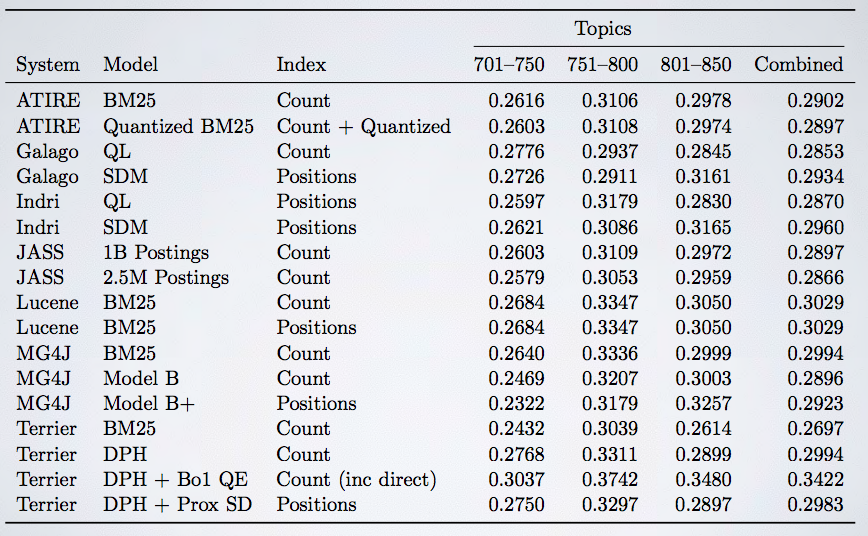
\includegraphics[width=0.5\textwidth]{images/l20-fig-2}
	\caption{Alcuni risultati (Mean Avarage Precision) ottenuti su TREC con il metodo proposto da RIGOR.}
\end{figure} 

\section{Valutazione delle performance - General Linear Mixed Model}

Posso combinare i dati dell'esecuzione dei vari sistemi della griglia in una matrice in cui le righe rappresentano i topic e le colonne sono i vari sistemi. Il valore delle cella è dato dall'average precision del sistema sul dato topic.
La matrice poi può essere plottata in una heat map (figura \ref{fig:heatmap}), in modo che sia più comprensibile.

\begin{figure}[htbp]
	\centering
	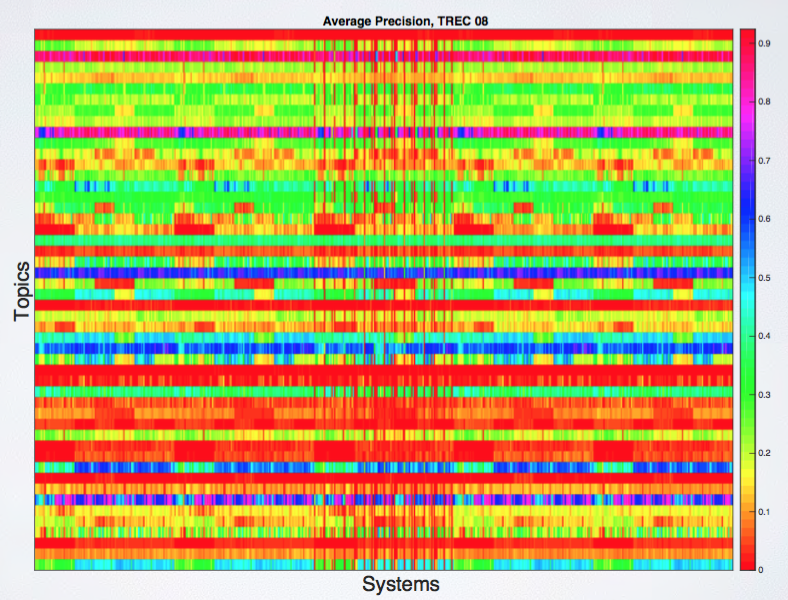
\includegraphics[width=0.5\textwidth]{images/l20-fig-3}
	\caption{Rappresentazione mediante heatmap della matrice. Nelle righe ci sono i topic mentre nelle colonne i vari sistemi.}\label{fig:heatmap}
\end{figure} 

Dalla figura \ref{fig:heatmap} si può notare che la variazione nella precisione è maggiore al variare dei topic, ovvero sistemi diversi tendono ad avere prestazioni simili sullo stesso topic.
Questo perché le performance del sistema dipendo sia dalla struttura del sistema, che dalla difficoltà del topic.

Pertanto si è pensato di modellare questa variazione della precisione con un \textbf{General Linear Mixed Model}, il quale spiega la variazione della variabile dipendente $Y$ nei termini della variabile indipendente, in questo caso il modello e di una varianza residua non controllata, che modella gli errori.

La scelta di questo modello è stata fatta perché gestisce variabili sia continue che categoriche (\textit{general}) che sono tra loro in combinazione lineare (\textit{linear}) e che dipendono da fattori sia fissi che casuali (\textit{mixed}).

Nel nostro caso lavoriamo con variabili di tipo categorico, perché anche se la MAP è un valore continuo a noi interessa la combinazione topic-sistema che è discreta.

Dobbiamo poi tener conto che questo deve poi essere applicato a degli esperimenti che possono essere considerati come indipendenti o ripetuti. Negli esperimenti \textbf{indipendenti} ogni soggetto viene provato con un fattore, mentre in quelli \textbf{ripetuti} su ogni soggetto vengono provati su tutti i fattori. Noi siamo nel caso ripetuto perché lo stesso topic viene provato su tutti i sistemi a disposizione.

Gli esperimenti possono poi essere \textbf{fattoriali} se tutti i fattori sono provati da tutti i soggetti oppure \textbf{nested} se per ogni soggetto viene provato solo un sotto-insieme delle possibili combinazioni di fattori. Noi siamo nel caso fattoriale.

I nostri modelli sono quindi a fattori fissi perché i topic sono finiti, con misure ripetute e combinazioni fattoriali.

Possiamo quindi modellare l'average precision con:

$$
Y_{ij} = \underbrace{\mu_{\cdot \cdot} + \tau_i + \alpha_j}_{Modello} + \underbrace{\epsilon_{ij}}_{Errore}
$$

\noindent dove:
\begin{itemize}
	\item $Y_{ij}$ è la variabile dipendente che voglio andare a stimare, ovvero nel nostro caso, l'average precision.
	\item $\mu_{\cdot\cdot}$ è la media di tutte le average precision (generale) che funziona come valore base ($\beta_0$, il valore dell'intercetta).
	\item $\tau_i$ è l'effetto del topic $i$.
	\item $\alpha_j$ è l'effetto del sistema $j$.
	\item $\epsilon_{ij}$ l'errore, ovvero tutto quello che il nostro modello non considera.
\end{itemize}

Il tutto poi può essere raccolto nella seguente tabella.

\begin{table}[htbp]
	\centering
	\begin{tabular}{llllll}
		\cline{2-5}
		\multicolumn{1}{l|}{}  & \multicolumn{1}{l|}{$ A_1 $} & \multicolumn{1}{l|}{$ A_2 $} & \multicolumn{1}{l|}{$ \ldots $} & \multicolumn{1}{l|}{$ A_p $} &  \\ \cline{1-5}
		\multicolumn{1}{|l|}{$ T'_1 $} & \multicolumn{1}{l|}{$ Y_{11} $} & \multicolumn{1}{l|}{$ Y_{12} $} & \multicolumn{1}{l|}{$ \ldots $} & \multicolumn{1}{l|}{$ Y_{1p} $} & $\mu_{1\cdot}$ \\ \cline{1-5}
		\multicolumn{1}{|l|}{$ T'_2 $} & \multicolumn{1}{l|}{$ Y_{21} $} & \multicolumn{1}{l|}{$ Y_{22} $} & \multicolumn{1}{l|}{$ \ldots $} & \multicolumn{1}{l|}{$ Y_{2p} $} & $\mu_{2\cdot}$ \\ \cline{1-5}
		\multicolumn{1}{|l|}{$\vdots$} & \multicolumn{1}{l|}{$\vdots$} 	 & \multicolumn{1}{l|}{$\vdots$}   & \multicolumn{1}{l|}{$ Y_{ij}$}  & \multicolumn{1}{l|}{$\vdots$}   & $\mu_{i\cdot}$ \\ \cline{1-5}
		\multicolumn{1}{|l|}{$ T'_n $} & \multicolumn{1}{l|}{$ Y_{n1} $} & \multicolumn{1}{l|}{$ Y_{n2} $} & \multicolumn{1}{l|}{$ \ldots $} & \multicolumn{1}{l|}{$ Y_{np} $} & $\mu_{n\cdot}$ \\ \cline{1-5}
		                               &      $\mu_{\cdot1}$             & $\mu_{\cdot2}$                  & $\mu_{\cdot j}$                 &   $\mu_{\cdot p}$               & $\mu_{\cdot\cdot}$
	\end{tabular}
	\caption{La matrice precedentemente osservata, rappresentata secondo il nostro modello. Le righe rappresentano i soggetti degli esperimenti ripetuti, nel nostro caso i topics, mentre le colonne rappresentano i fattori, ovvero i sistemi di IR.}
	\label{my-label}
\end{table}

Ovviamente questo è solamente il modello, restano ancora da stimare i vari parametri del modello, per fare la validazione del modello.

\subsection{Stima dei parametri del modello}

Siamo quindi in una situazione nella quale riusciamo ad osservare la variabile dipendente $Y_{ij}$ con i nostri esperimenti e dobbiamo stimare i parametri del nostro modello.

Si ha quindi che la media totale $\mu_{\cdot \cdot}$ può essere stimata con la media aritmetica di tutte le celle della matrice, ovvero:

$$
\hat{\mu}_{\cdot \cdot} = \frac{1}{pn}\sum\limits_{j=1}^{p}\sum\limits_{i=1}^{n} Y_{ij}
$$

Per stimare i vari effetti dei singoli topic e dei singoli sistemi posso utilizzare le medie marginali, rimuovendo l'andamento generale dato da $\hat{\mu}_{\cdot \cdot}$.
Quindi:

\begin{align*}
	\hat{\mu}_{i\cdot} & \frac{1}{p}\sum\limits_{j=1}^{p} Y_{ij} \qquad \hat{\tau} = \hat{\mu}_{i\cdot} - \hat{\mu}_{\cdot\cdot} \\
	\hat{\mu}_{\cdot j} &= \frac{1}{n}\sum\limits_{i=1}^{n} Y_{ij} \qquad \hat{\alpha} = \hat{\mu}_{\cdot j} - \hat{\mu}_{\cdot\cdot}
\end{align*}

Possiamo quindi utilizzare il nostro modello stimato per effettuare la stima dell'average precision:

$$
\hat{Y}_{ij} = \hat{\mu}_{\cdot\cdot} + \hat{\tau}_i + \hat{\alpha}_j = \hat{\mu}_{i\cdot} + \hat{\mu}_{\cdot j} - \hat{\mu}_{\cdot\cdot}
$$

con il quale possono andare ad effettuare anche una stima dell'errore commesso dal modello:

$$
\hat{\epsilon}_{ij} = Y_{ij} - \hat{Y}_{ij} = Y_{ij} - (\hat{\mu}_{i\cdot} + \hat{\mu}_{\cdot j} - \hat{\mu}_{\cdot\cdot})
$$









	% !TEX encoding = UTF-8
% !TEX TS-program = pdflatex
% !TEX root = computabilità e algoritmi.tex
% !TEX spellcheck = it-IT

\chapter{Esercizi in preparazione al parziale}


\section{Teorema SMN}

\subsection{Esercizio 1}

Dimostrare che esiste $ S : \mathbb{N} \rightarrow \mathbb{N}$ tale che $|\: W_{S(x)}\:|  = 2 x$ e $ |\: E_{S(x)}\:| =x $

\subsubsection{Soluzione}

Si cerca una funzione $ f(x,y) $ che con $ x $ fissato abbia esattamente le caratteristiche richieste, ci pensa il teorema SMN a fare il resto.

\begin{align*}
f(x,y) &= \begin{cases}
y \dotminus x, &\text{ se } y < 2x \\
\uparrow, &\text{altrimenti}
\end{cases} \\
 &= y\dotminus x + \underbrace{\mu z. y +1 -2x}_{\text{fa divergere se } y \geq 2x}
\end{align*}

Questa funzione è calcolabile e quindi per il teorema SMN esiste $ S : \mathbb{N} \rightarrow \mathbb{N} $ tale che 

$$
\phi_{S(x)}(y) = f(x,y)
$$

e per costruzione $W_{S(x)} = [0,2x-1]$ e $ E_{S(x)} = [0,x-1] $.

\section{Calcolabilità delle funzioni}

\subsection{Esercizio 1}

Dimostrare che 

$$
f(x) = \begin{cases}
\phi_x(x) &\text{se} \phi_x(x)\downarrow \\
0 &\text{altrimenti}
\end{cases}
$$

non è calcolabile.

\subsubsection{Soluzione}

Non si può usare il \textit{trick} della diagonale, perché la funzione deve essere proprio uguale alla diagonale.

$$ h(x) = f(x)+1 = \begin{cases}
\phi_x(x)  + 1 &\text{se} \phi_x(x)\downarrow \\
1 &\text{altrimenti}
\end{cases}
 $$

Così facendo $ h \neq \phi_x(x) \forall x $ e pertanto non è calcolabile.

Ma $ h $ è il successore di $ f $, quindi $ f $ non può essere calcolabile, perché se così non fosse $ h(x) = f(x) +1 $ sarebbe calcolabile per composizione di funzioni calcolabili.ò

Da notare che questa cosa non vale in se e solo se:

$$ h(x) = f(x) +1 \text{ non calcolabile }\Rightarrow f(x)  \text{ non calcolabile } $$

ma \textbf{NON \`{E} VERO}

$$ f(x) \text{ non calcolabile } \Rightarrow f(x) = h(x) +1 \text{ non calcolabile }$$
%------------

\subsection{Esercizio 2}

Sia $ \mathbb{P} $ l'insieme dei numeri pari, dimostrare che la funzione caratteristica è primitiva ricorsiva.

$$
\mathcal{X}_\mathbb{P} = \begin{cases}
1 &\text{ se $ x $ è pari} \\
0 &\text{ altrimenti}
\end{cases}
$$

\subsubsection{Soluzione}

\begin{align*}
\mathcal{X}_\mathbb{P}(0) &= 1
\mathcal{X}_\mathbb{P}(x+1) &= \overline{sg}\big(\mathcal{X}_\mathbb{P}(x)\big)
\end{align*}

Dal momento che in un esercizio non sappiamo dell'esistenza del segno negato è necessario andare a mostrare che anche quella funzione è primitiva ricorsiva:

\begin{align*}
 \overline{sg}(0) &= 1 \\
  \overline{sg}(x+1) &= 0
\end{align*}


\subsection{Esercizio 3}

Dimostrare che la funzione $ half(x) = \lfloor\frac{x}{2}\rfloor $ è primitiva ricorsiva.

\subsubsection{Soluzione}

\begin{align*}
half(0) &= 0 \\
half(x+1) &= half(x) + rm_2(x)
\end{align*}

come prima bisogna dimostrare che $ rm_2 $ è ricorsiva primitiva

\begin{align*}
rm_2(x) &= 0
rm_2(x+1) &= \overline{sg}(rm_2(x))
\end{align*}

ma anche $ \overleftarrow{sg} $ è in $ \mathcal{PR} $

\begin{align*}
\overline{sg}(0) &= 1 \\
\overline{sg}(x+1) &= 0
\end{align*}

\section{Macchina URM}

\subsection{Esercizio 1}

Consideriamo la macchina $ \text{URM}^- $ che al posto dell'istruzione successore ha quella che effettua il predecessore.
Come sono in relazione le due classi? 

Ovvero:
 $$\mathcal{C}^- \text{ ? } \mathcal{C}$$
 
 \subsubsection{Soluzione}
 
 \`{E} chiaro che  $\mathcal{C}^- \subseteq \mathcal{C}$ perché la funzione predecessore può essere sostituita da un programma che calcola il predecessore.
 
 Per vedere \textbf{se}  $\mathcal{C}^- \supseteq \mathcal{C}$ bisogna provare a simulare il successore con un programma per la macchina $ \text{URM}^- $.

Ma dato un $ P \in \text{URM}^- $ qualsiasi $ P(\vec{x}) $ dopo $ n $ passi, $ \forall n $, tutti i registri $ r_i \leq \max x_i$.

Se $ n = 0 $ è ovvio perché i registri non cambiano.

Se $ n \rightarrow n+1 $, l'istruzione aggiunta può essere:
\begin{itemize}
	\item precessore ma il valore non aumenta
	\item zero azzera un registro
	\item il trasferimento non incrementa i valori
\end{itemize}

Dal momento che i registri di un programma in $ \text{URM}^- $ non aumentano mai, non è possibile implementare la funzione successore, quindi \textbf{non vale} la relazione $\mathcal{C}^- \supseteq \mathcal{C}$.


\subsection{Esercizio 2}
$ \text{URM}^S$ che non ha \texttt{S(n)} e \texttt{J(m,n,t)} ma ha \texttt{JS(m,n,t)} che prima fa il test e poi incrementa il registro $ m $.

\subsubsection{Soluzione}

$\mathcal{C}^S \subseteq \mathcal{C}$ perché un programma URM riesce ad emulare l'istruzione \texttt{JS}.

$\mathcal{C}^S \supseteq \mathcal{C}$ non vale, perché un programma $ \text{URM}^S$ non riesce a calcolare la funzione successore.


\section{Diagonalizzazione}

\subsection{Esercizio 1}

$ F_0 = \{f \: | \: \text{cod}(f) \subseteq \{0\} \text{ e parziali}\}$ è numerabile?

\subsubsection{Soluzione}

L'unica differenza tra queste funzioni è data dai domini che sono tanti quanti i numeri naturali.

Suppongo per assurdo che $ F_0 $ sia enumerabile, allora:

\begin{verbatim}
		f0	f1 f2
0      0   0   0
1      0   0
2
\end{verbatim}

considerando la diagonale, posso definire

$$
f(x) = \begin{cases}
0 &\text{se } f_x(x)\uparrow \\
\uparrow &\text{se } f_x(x)=0
\end{cases}
$$

$ f $ dovrebbe appartenere a $ F_0 $ ma per costruzione non compare nella enumerazione, quindi $ F_0 $ non è enumerabile.

\subsection{Esercizio 2}

$ f : \mathbb{N} \rightarrow \mathbb{N} $ totale e decrescente se $ \forall x,y \: x \leq y \Rightarrow f(y) \leq f(x) $.

$ F_d = \{ f : \mathbb{N} \rightarrow \mathbb{N} \: \ \: f \text{ totale e descrescente e } \text{cod}(f) \subseteq \{0,1\} \} $ è numerabile?

\subsubsection{Soluzione}

Le funzioni dell'insieme possono essere o costanti uguali a 0 o 1, oppure uguali a 1 fino ad un certo valore per poi diventare costanti a 0.

$$ \forall f \in F_d \: n(f)  = \text{sup}(\{x \: | \: f(x) = 1\})$$

$ n(f) $ è il punto in cui cambia il valore della funzione e caratterizza $ f $, ovvero

$$
\forall f_1, f_2 \in F_d \: n(f_1) = n(f_2) \Rightarrow f_1 = f_2
$$

quindi $ n : F_d \rightarrow \mathbb{N} \cup \{\infty\} $ è una funzione iniettiva e suriettiva, pertanto $ |\: F_d \:| = |\: \mathbb{N} \cup \{ \infty \} \:| $, ovvero $ F_d $ è numerabile.


\subsection{Esercizio 3}

Trovare $ f : \mathbb{N} \rightarrow \mathbb{N} $ totale e non calcolabile tale che $ f(x)  =x $ per infiniti $ x $.

\subsubsection{Soluzione}

$$
f(x) = \begin{cases}
x, &\text{ se $ x $ è pari} \\
\phi_{\frac{x-1}{2}}(x) +1, &\text{ se } \phi_{\frac{x-1}{2}}(x) \downarrow \\
0, &\text{ se } \phi_{\frac{x-1}{2}}(x) \uparrow 
\end{cases}
$$

\subsection{Esercizio 4}

Trovare una funzione $ f $ crescente, totale e non calcolabile.

\subsubsection{Soluzione}

$$
h(x) = \begin{cases}
\phi_x(x)+1, &\text{ se }\phi_x(x)\downarrow \\
0, &\text{ se } \phi_x(x) \uparrow
\end{cases}
$$

$ h $ è non calcolabile perché è definita sulla diagonale distorta.

$$
f(x) = \sum\limits_{y \leq x} h(y)
$$

Così definita $ f $ è:
\begin{itemize}
	\item totale
	\item crescente: $ f(x+1) = f(x) + h(x+1) \geq f(x) $
	\item $ \forall x $ se $ \phi_x(x) \downarrow \: f(x) = \sum\limits_{y \leq x} h(y) \geq h(x) = \phi_x(x) +1 \neq \phi_x(x) $ e se $ \phi_x(x) \uparrow $, $ h(x) = 0 \neq \phi_x(x) $, ovvero $ f $ non è calcolabile.
\end{itemize}

\subsection{Esercizio 5}

Può esistere $ f : \mathbb{N} \rightarrow \mathbb{N} $ non calcolabile tale che $ \forall g : \mathbb{N} \rightarrow \mathbb{N} $ non calcolabile $ f+g  $ è calcolabile?

$$
(f+g)(x) = f(x) + g(x)
$$

\subsubsection{Soluzione}

Non può esistere, perché per assurdo, sia $ f $ una funzione tale che $ (f+f) $ è calcolabile:

\begin{align*}
h(x) &= f(x) + f(x) \\
		&= 2 f(x)
\end{align*}

$h(x)$ è quindi calcolabile, però utilizzando questa funzione si può definire $ f(x) = qt(2, h(x)) $, dimostrando la calcolabilità di $ f $ che per ipotesi non è calcolabile.



	\appendix
	\chapter{Esami vecchi}
	% !TEX encoding = UTF-8
% !TEX program = pdflatex
% !TEX root = InformationRetrieval.tex
% !TEX spellcheck = it-IT

\section{Esame 2016-07-05}

\subsection{Domanda 1}

L'indicizzazione automatica dei documenti testuali si basa sulla capacità di discriminare il contenuto in funzione della frequenza dei termini, come indicato da Luhn. Si illustri questo concetto che sta alla base della rappresentazione dei contenuti della rappresentazione testuale.

\subsubsection{Soluzione}

Secondo Luhn è possibile individuare un sotto-insieme di parole limitato che compaiono molto frequentemente all'interno dei documenti della collezione e un sotto-insieme di parole molto più grande che contiene le parole che appaiono meno frequentemente.
Le parole di questo secondo sotto-insieme possono essere usate per discriminare il contenuto informativo dei documenti in cui compaiono, stando però attenti agli errori di battitura.

Zipf ha formalizzato la distribuzione di questi termini, fornendo un modello: come prima cosa è necessario calcolare tutte le occorrenze dei vari termini, per poi ordinarli per frequenza decrescente, assegnando rango massimo al termine più frequente. Così facendo si ha che

$$
r \times tf_r = k
$$

Luhn ha quindi proposto di determinare due soglie di cut-off e di rimuovere durante l'indicizzazione tutte le parole che hanno frequenza superiore alla soglia massima, per rimuovere le parole scarsamente informative, e tutte quelle con frequenza inferiore alla soglia minima per evitare gli errori di battitura. Viene quindi presa in considerazione solamente la "\textit{parte centrale}" dell'iperbole di Zipf, ovvero le parole che hanno un resolving power maggiore (capacità di discriminare il contenuto di un documento).

\subsection{Domanda 2}

Siano dati i seguenti documenti testuali

\begin{itemize}
	\item \textbf{D1}: Il codice sorgente esprime l'algoritmo del programma tradotto nel linguaggio di programmazione.
	\item \textbf{D2}: Un programma è un insieme di istruzioni che, una volta eseguite, produce soluzione per una data classe di problemi.
	\item \textbf{D3}: Con il termine istruzione in informatica si intende il comando impartito ad un esecutore utilizzando un linguaggio ad esso comprensibile
\end{itemize}

Si effettui la loro indicizzazione automatica creando l'indice dei descrittori. Si descriva una possibile strategia per la costruzione di una stop list corrispondente ai documenti forniti.

\subsubsection{Soluzione}

L'indicizzazione automatica è composta dalle seguenti fasi:
\begin{enumerate}
	\item Analisi lessicale/tokenizzazione
	\item Rimozione delle stop word
	\item Stemming
	\item Composizione dei termini
\end{enumerate}

\paragraph{Fase 1: Analisi lessicale}

Creo i token, considerando come separatore ``,``, ``.'',``''' e lo spazio, rimuovo i separatori e rendo tutto minuscolo.

\begin{itemize}
	\item \textbf{D1}: algoritmo codice del di esprime il l linguaggi nel programma programmazione sorgente
	\item \textbf{D2}: che classe data di di è eseguite insieme istruzioni problemi produce programma soluzione un un una una
	\item \textbf{D3}: ad ad comando comprensibile con esecutore esso il il impartito in informatica intende linguaggio si termine un un utilizzando  
\end{itemize}

\paragraph{Fase 2: rimozione delle stopword}

Come stop word è possibile considerare tutte le parole funzionali della lingua della collezione, in questo caso l'italiano, così come si possono applicare le indicazioni di Luhn, andando a scartare, e quindi considerare come stop word, le parole tanto frequenti e le parole poco frequenti.

In questo caso, tutte le parole sarebbero poco frequenti, quindi vengono rimosse solamente quelle funzionali.

\begin{itemize}
	\item \textbf{D1}: algoritmo codice esprime linguaggio programma programmazione sorgente
	\item \textbf{D2}: classe data eseguite insieme istruzioni problemi produce programma soluzione
	\item \textbf{D3}: comando comprensibile esecutore impartito informatica intende linguaggio termine utilizzando
\end{itemize}

\paragraph{Fase 3: Stemming} 

Lo stemming consiste nel ridurre i termini ad una radice comune, in modo da raggruppare le forme varianti di una parola in un unico termine. Ci sono vari modi di algoritmi di stemming, alcuni generici e altri specifici per una determinata lingua. In alternativa si possono usare dei dizionari creati da persone esperte. Durante questa fase bisogna stare attenti a non stemmare troppo o troppo poco.

Per motivi pratici, lo stemming viene fatto riducendo le parole tutte alla forma singolare, i verbi alla forma infinita e abbreviando sia ``programma'' che ``programmazione'' in ``programm''.

\begin{itemize}
	\item \textbf{D1}: algoritmo codice esprimere linguaggio programm programm sorgente
	\item \textbf{D2}: classe data eseguire insieme istruzione problema produrre programm soluzione
	\item \textbf{D3}: comando comprensibile esecutore impartire informatica intendere linguaggio termine utilizzare
\end{itemize}

\paragraph{Fase 4: Composizione dei termini}

In questa fase alcuni termini che hanno senso solo se compaiono in una determinata sequenza vengono composti tra loro, creando dei nuovi termini. Questa cosa è computazionalmente onerosa e pertanto raramente viene fatta. In questo caso non consideriamo questa fase

\paragraph{Fase 5: Creazione dell'indice}

L'indice può essere fatto considerando gli stem oppure i termini non stemmati e allo stesso modo può contenere un valore binario o con la frequenza con la quale gli stem compaiono nel documento.
In questo caso viene scelto di usare gli stem con la frequenza.
L'indice risultante è riportato in tabella \ref{ex:index}

\begin{table}[htpb]
	\centering
	\caption{Indice}
	\label{ex:index}
\begin{tabular}{c|c|c|c|c|c|c|c|}
	\cline{2-8}
	& \multicolumn{3}{c|}{\textbf{Documenti}} & \multicolumn{4}{c|}{\textbf{(cont'd)}}                     \\ \hline
	\multicolumn{1}{|c|}{\textbf{Termini}} & \textbf{D1} & \textbf{D2} & \textbf{D3} & \textbf{Termini} & \textbf{D1} & \textbf{D2} & \textbf{D3} \\ \hline
	\multicolumn{1}{|c|}{algoritmo}        & 1           & 0           & 0           & istruzione       & 0           & 1           & 0           \\ \hline
	\multicolumn{1}{|c|}{classe}           & 0           & 1           & 0           & intendere        & 0           & 0           & 1           \\ \hline
	\multicolumn{1}{|c|}{codice}           & 1           & 0           & 0           & linguaggio       & 1           & 0           & 1           \\ \hline
	\multicolumn{1}{|c|}{comando}          & 0           & 0           & 1           & problema         & 0           & 1           & 0           \\ \hline
	\multicolumn{1}{|c|}{comprensibile}    & 0           & 0           & 1           & produrre         & 0           & 1           & 0           \\ \hline
	\multicolumn{1}{|c|}{esecutore}        & 0           & 0           & 1           & programm         & 2           & 1           & 0           \\ \hline
	\multicolumn{1}{|c|}{eseguire}         & 0           & 1           & 0           & soluzione        & 0           & 1           & 0           \\ \hline
	\multicolumn{1}{|c|}{esprimere}        & 1           & 0           & 0           & sorgente         & 1           & 0           & 0           \\ \hline
	\multicolumn{1}{|c|}{impartire}        & 0           & 0           & 1           & termine          & 0           & 0           & 1           \\ \hline
	\multicolumn{1}{|c|}{informatica}      & 0           & 0           & 1           & utilizzare       & 0           & 0           & 1           \\ \hline
\end{tabular}
\end{table}

\subsection{Domanda 3}

Si considerino i due documenti

\begin{itemize}
	\item \textbf{D1} $(0.7, 0.2, 0.1, 0.5)$
	\item \textbf{D2} $(0.9, 0.4, 0.2, 0.2)$
\end{itemize}

Indicizzati da quattro termini dove i valori indicano i pesi associati ai termini.

Sia data la query $Q = (1.0, 1.2, 0.1, 0)$ indicizzata dagli stessi termini. Si calcolino le misure "coseno" per i due documenti.

\subsubsection{Soluzione}

\begin{align*}
S(D1, Q) &= \frac{
	\sum_j d_{ij}q_j
}{
	\sqrt{\sum_j d_{ij}^2}\sqrt{\sum_j q_{j}^2}
} \\
&= \frac{
	0.7\cdot 1.0 + 0.2 \cdot 1.2 + 0.1 \cdot 0.1 + 0.5 \cdot 0
}{
 \sqrt{(0.49 + 0.04 + 0.01 + 0.25)} \sqrt{(1 + 1.04 + 0.01 + 0)}
}\\
&= \frac{0.7 + 0.24 + 0.05}{\sqrt{0.79} \cdot \sqrt{2.05}} = \frac{0.99}{0.88 \cdot 1.43} = 0.7
\end{align*}

\begin{align*}
S(D1, Q) &= \frac{
	\sum_j d_{ij}q_j
}{
	\sqrt{\sum_j d_{ij}^2}\sqrt{\sum_j q_{j}^2}
} \\
&= \frac{
	0.9 + 0.48+ 0.02
}{
	\sqrt{0.81 + 0.16 + 0.04 + 0.04}\cdot 1.43
}\\
&= \frac{
	1.4
}{
	\sqrt{1.05}\cdot 1.43
} = \frac{1.4}{1.46} = 0.96
\end{align*}

\subsection{Domanda 4}

Si definisca cos'è un agente web; si descrivano i componenti e i compiti che svolge un web crawler.

\subsubsection{Soluzione}

Un agente web o crawler è un programma che ``esplora'' il web per scaricare le varie pagine (e/o contenuti multimediali) in modo che possano essere indicizzate da un sistema di information retrieval.
La ``navigazione'' del crawler parte da una lista di URL che prendere il nome di lista di seed e prosegue seguendo i link presenti nelle pagine visitate dal crawler.

Un crawler è composto da vari elementi:

\begin{itemize}
	\item \textbf{Coda di URL}: è una coda a priorità che contiene gli URL che il crawler deve ancora visitare. La priorità di un URL è dinamica in quanto si può scegliere di far aumentare la priorità di un URL se questo viene trovato su più pagine oppure se lo si vuole rivisitare più in fretta. Questo perché se una pagina che viene aggiornata frequentemente è tanto indietro nella coda, magari possono venire perse delle informazioni utili all'utente del sistema e pertanto viene fatta ``saltare la fila'' all'URL. L'implementazione di questa coda non è banale, perché gli URL sono delle stringhe e quindi occupano svariati byte in memoria e, date le dimensioni del web, la coda si popola molto velocemente.
	\item \textbf{DNS translator}: gli URL sono relativi ad un dominio, ma per poter contattare il server è necessario conoscere l'IP, serve quindi un componente che si occupa di dialogare con un DNS per tradurre il dominio in un IP. Dato che i DNS non sono pensati per rispondere ad alte velocità, è necessario configurare il crawler in modo che mandi richieste troppo velocemente, altrimenti si rischia di far le richieste del crawler come un tentativo di attacco DoS. Per velocizzare il processo si può mantenere una cache delle traduzioni, perché durante la visita di un sito, il dominio, pertanto il server con le pagine è sempre quello e quindi basta richiedere la traduzione dell'indirizzo una sola volta. \`E inoltre ragionevole pensare che nel breve periodo l'IP associato ad un dominio non cambi, quindi la cache può essere mantenuta per un certo periodo di tempo, solo che ogni tanto deve essere comunque aggiornata.
	\item \textbf{Robot-protocol interpreter}: tipicamente i server contengo un file \texttt{robot.txt} che definisce delle limitazioni per i crawler. Serve quindi un componente che sia in grado di interpretare il file. Ad esempio il file può ``vietare'' l'accesso a determinate aree del sito, oppure definire un intervallo temporale alle richieste delle pagine per evitare di intasare il server e rovinare l'esperienza degli utenti normali. Nessuno obbliga a rispettare tali norme, ma è fortemente consigliato, per evitare che il server blocchi l'IP del crawler.
	\item \textbf{Processatore delle pagine}: dopo aver tradotto l'url e interpretato il \texttt{robot.txt}, si può scaricare la pagina. Una volta che questa è scaricata viene passata al sistema di IR in modo che venga indicizzata. La pagina però deve essere anche esaminata dal crawler, in modo da identificare eventuali URL da reinserire in coda (oppure si può scegliere di non reinserirli, perché troppo profondi nella gerarchia del sito) . C'è da prestare attenzione anche all'eventuale meta tag \texttt{no-index} o alle ancore marcate come \texttt{no-follow}. Infine, la pagina potrebbe contenere del JavaScript (o altro) che reindirizza l'utente su un'altra pagina oppure che carica dinamicamente il contenuto via AJAX oppure che contiene frame html, c'è quindi la necessità che il crawler sia in grado di distinguere questi casi e, a scelta dello sviluppatore, di gestirli.
\end{itemize}

\subsection{Domanda 5}

\begin{enumerate}
	\item Si definiscano le misure 11-Point Average Precision e Average Precision e si descrivano le principali caratteristiche (vantaggi e svantaggi) delle due misure di efficacia.
	\item Si definisca il concetto di recall base.
	\item Si definiscano le misure di Precisione a cut-off 10 e di precisione alla recall base e se ne descrivano le principali differenze.
\end{enumerate}

\subsubsection{Soluzione}

\begin{enumerate}
	\item 11-Point AP è la media delle precisioni interpolate sugli 11 punti di recall. Ovvero sia $RP=\{0, 0.1, \ldots 1\}$ un insieme di valori di recall e $rp \in RP$ un punto dell'insieme. La precisione interpolata in quel punto di recall è definita come:
	$$
	IP_{rp} = \max\limits_{1 \leq r \leq N | rec@r \geq rp} prec@r
	$$
	
	ovvero come il massimo valore di precisione con cut-off al ragno $r$, tale che la recall al rango $r$ sia maggiore o uguale al valore del punto $rp$.
	
	L'11-pt AP è quindi definita come la media aritmetica dei vari valori di $IP_{rp}$ per $rp \in RP$.
	
	$$
	11AP = \frac{1}{11}\sum\limits_{rp \in RP} IP_{rp}
	$$
	
	L'average precision è invece la media alla recall-base di tutti i valori di precisione con cut-off a $r$, moltiplicati per il peso del giudizio di rilevanza binario del documento di rango $r$, ovvero:
	
	\begin{align*}
	AP &= \frac{1}{RB} \sum\limits_{r = 1}^{N} \tilde{\mathbf{r}}_t[r]\cdot prec@r \\
	&= \frac{1}{N} \sum\limits_{r = 1}^{N} \tilde{\mathbf{r}}_t[r]\cdot \frac{\sum\limits_{j = 1}^{r} \tilde{\mathbf{r}}_t[r]}{r}
	\end{align*}
	
	La prima misura nasce come versione quantitativa della curva richiamo-precisione e permette di confrontare due run distinte per uno stesso topic, pesando allo stesso tutti i valori di precisione interpolata.
	
	L'AP permette sempre di valutare due run diverse, con la differenza che viene dato maggior peso ai documenti rilevanti che si trovano alle posizioni più alte del rank. Questo perché se il rank è alto, la precisione a quel valore di rank sarà maggiore rispetto a quella in posizioni più basse.\todo{altro?}
	
	\item La recall base per un topic $t$ è il numero di documenti rilevanti presenti nella collezione. Formalmente, sia $REL$ un insieme di giudizi di rilevanza totalmente ordinato, $GT$ la ground-truth, allora $RB$ è una funzione tale che
	
	\begin{align*}
		RB:&T \to \mathbb{N} \\
			& t \to RB_t =  |\{ d \in D | min(REL) \prec GT(d, REL) \}|
	\end{align*}

	\item La precisione con cut-off a $k$ è la precisione calcolata sui primi $k$ elementi di rango massimo della run.
	
	$$
	prec@k = \frac{\sum\limits_{r = 1}^{k} \tilde{\mathbf{r}}_t}{k}
	$$
	
	$prec@10$ è quindi la precisione sui primi 10 documenti recuperati, mentre $prec@RB_t$ è la precisione considerando tanti documenti quanti ce ne sono nella recall base per quel dato topic.
	
	Entrambe le misure sono simili in quanto sono casi di $prec@k$, solo che la prima può essere migliore per confrontare sistemi di reperimento che lavorano in ambito web (tipicamente la SERP contiene 10 elementi), mentre la seconda è più generica e simile al richiamo: se $prec@RB_t$ è 1 vuol dire che ho trovato tutti i documenti rilevanti e li ho messi nelle prime posizioni della run (la run completa può comunque essere più lunga e avere documenti non rilevanti), se invece ho che la $prec$ normale è 1, vuol dire che il sistema ha trovato esattamente tutti i documenti rilevanti. \todo{c'è altro da dire?}
	
\end{enumerate}

	% !TEX encoding = UTF-8
% !TEX program = pdflatex
% !TEX root = InformationRetrieval.tex
% !TEX spellcheck = it-IT

\section{Esame 2016-09-06}

\subsection{Domanda 1}

Data una collezione testuale di 7 documenti

\begin{table}[htbp]
	\centering
	
	\begin{tabular}{c|c|c|c|}
		\cline{2-4}
		& \textbf{$t_1$}                                 & \textbf{$t_2$}                                 & \textbf{$t_3$}                                 \\ \hline
		\rowcolor[HTML]{EFEFEF} 
		\multicolumn{1}{|c|}{\cellcolor[HTML]{EFEFEF}{\color[HTML]{32CB00} $d_1$}} & {\color[HTML]{32CB00} 1}                      & {\color[HTML]{32CB00} 0}                      & {\color[HTML]{32CB00} 2}                      \\ \hline
		\rowcolor[HTML]{EFEFEF} 
		\multicolumn{1}{|c|}{\cellcolor[HTML]{EFEFEF}$d_2$}                        & 0                                             & 5                                             & 1                                             \\ \hline
		\rowcolor[HTML]{EFEFEF} 
		\multicolumn{1}{|c|}{\cellcolor[HTML]{EFEFEF}{\color[HTML]{32CB00} $d_3$}} & {\color[HTML]{32CB00} 2}                      & {\color[HTML]{32CB00} 0}                      & {\color[HTML]{32CB00} 2}                      \\ \hline
		\rowcolor[HTML]{EFEFEF} 
		\multicolumn{1}{|c|}{\cellcolor[HTML]{EFEFEF}$d_4$}                        & 0                                             & 3                                             & 1                                             \\ \hline
		\multicolumn{1}{|c|}{$d_5$}                                                & 3                                             & 0                                             & 1                                             \\ \hline
		\multicolumn{1}{|c|}{$d_6$}                                                & 2                                             & 2                                             & 0                                             \\ \hline
		\multicolumn{1}{|c|}{{\color[HTML]{32CB00} $d_7$}}                         & {\color[HTML]{32CB00} 3} & {\color[HTML]{32CB00} 2} & {\color[HTML]{32CB00} 1} \\ \hline
	\end{tabular}
\end{table}

Stimare i parametri del BIM utilizzando $d_1,d_2, d_3$ e $d_4$ come documenti di training. Sappiamo inoltre che per la query $\{t_2, t_3\}$ risultano rilevanti $d_1$, $d_3$ e $d_7$.

Calcolare:

\begin{enumerate}
	\item $p_i$ e $q_i$, tenendo conto che $N_R = N_{NR} = 2$
	\item $P(\rel | d,q)$ per i documenti di test utilizzando il classico $relevance \ weight = \log\bigg(\cfrac{p_i}{1-p_i} \cfrac{1- q_i}{q_i}\bigg)$
	\item la lista ordinata per rilevanza.
\end{enumerate}

\subsubsection{Soluzione}



%  \log(\frac{p_i+0.5}{1-p_i+0.5} \frac{1-q_i+0.5}{q_i+0.5}) 

\begin{enumerate}
	\item 
	$$
	\boxed{p_i = \frac{N_{t_iR} + \alpha_i}{N_R + \alpha_i + \beta_i}} \quad \text{e} \quad \boxed{q_i = \frac{N_{t_iNR} + \alpha_i}{N_{NR} + \alpha_i + \beta_i}}
	$$
	
	con $\alpha_i = \beta_i = 0.5$ che deriva da \ref{eq:smoothing}.
	\begin{itemize}
		\item $p_1 = \cfrac{N_{t_iR} + 0.5}{N_R + 0.5 + 0.5} =\cfrac{2 + 0.5}{2 + 0.5 + 0.5} = \cfrac{5}{6} \qquad q_1 = \cfrac{0 + 0.5}{2 + 0.5 + 0.5} = \cfrac{1}{6}$
		\item $p_2 = \cfrac{1}{6} \qquad q_2 = \cfrac{5}{6}$
		\item $p_3 = \cfrac{5}{6} \qquad q_3 = \cfrac{5}{6}$
	\end{itemize}
	\item In questo caso posso o usare i $p_i$ e $q_i$ precedentemente calcolati:
	
	$$P(\rel|d,q) \propto_q \sum_{i \in q \cap d}w_i = \sum_{i \in q \cap d}\log\bigg(\cfrac{p_i}{1-p_i} \cfrac{1- q_i}{q_i}\bigg)$$
	
	oppure utilizzare la formula \ref{eq:wrsj}.
	\begin{itemize}
		\item $P(\rel | d_5, q) \propto \log\bigg(\cfrac{p_3}{1-p_3}\cfrac{1-q_3}{q_3}\bigg) = \log\bigg(\cfrac{\frac{5}{6}}{1-\frac{5}{6}}\cfrac{1-\frac{5}{6}}{\frac{5}{6}}\bigg) = \log(1) = 0 $ Da notare che ha senso perché $t_3$ compare in tutti i documenti di training e quindi non è significativo.
		\item $P(\rel | d_6, q) \propto \log\bigg(\cfrac{p_2}{1-p_2}\cfrac{1-q_2}{q_2}\bigg) = \log\bigg(\cfrac{\frac{1}{6}}{1-\frac{1}{6}}\cfrac{1-\frac{5}{6}}{\frac{5}{6}}\bigg) = \log\bigg(\cfrac{1}{25}\bigg)$. 
		\item $P(\rel | d_7, q) \propto \log\bigg(\cfrac{p_3}{1-p_3}\cfrac{1-q_3}{q_3}\bigg) +\log\bigg(\cfrac{p_2}{1-p_2}\cfrac{1-q_2}{q_2}\bigg) = \log\bigg(\cfrac{1}{25}\bigg)+ \log(1)= \log\bigg(\cfrac{1}{25}\bigg)$
	\end{itemize}
	\item La lista ordinata è quindi $d_5, d_6, d_7$ e questo in qualche modo a senso, perché per le informazioni che ha a disposizione il modello, si ha che $t_3$ non discrimina perché è presente su tutti, $t_2$ compare solo sui non rilevanti e $t_1$ compare solo sui rilevanti. Quindi la presenza di $t_1$ aumenta lo score del documento, la presenza di $t_2$ lo abbassa e la presenza di $t_3$ non lo modifica. 
	Pertanto, siccome la query contiene solo $t_2$ e $t_3$ il ranking viene fatto senza considerare $t_1$ nel calcolo dello score. Quindi rank più alto viene dato a $d_5$, perché non contiene $t_2$ e poi seguono $d_6$ e $d_7$ che sono penalizzati per la presenza di $t_2$.
\end{enumerate}


\subsection{Domanda 2}

Quali sono le differenze più significative fra il reperimento delle informazioni su collezioni di documenti testuali disponibili localmente e per il reperimento web?

\subsubsection{Soluzione}

Le collezioni testuali sono più statiche, è difficile che una volta che un documento è stato indicizzato il suo contenuto cambi. Quindi l'indicizzazione di una collezione locale viene fatta una sola volta e ogni tanto si aggiorna l'indice. 
Si riesce inoltre ad avere un'idea precisa della dimensione della collezione e dell'autorevolezza dei documenti che contiene. 

Nel web i documenti sono le singole pagine, ce ne sono tante e possono cambiare molto rapidamente, è quindi necessario aggiornare in continuazione l'indice. Non è garantita l'autorevolezza della collezione e non è nota la dimensione della collezione, quindi è difficile stimare le risorse (tempo e spazio) necessarie per indicizzarla. Le pagine però sono strutturate con i tag html i quali possono essere usati per valorizzare in modo diverso i termini contenuti nella pagina.

Sempre in termini di risorse, nell'ambito Web è necessario tenere conto della banda necessaria e del tempo che serve per scaricare una pagina, la quale può trovarsi in un angolo remoto del modo. Dopo aver scaricato le pagine è necessario inoltre avere sufficiente spazio per tenerle tutte in memoria. Con i documenti testuali invece non c'è bisogno di tenere conto della banda, perché al massimo è una risorsa che viene utilizzata una tantum, solamente per recuperare la prima volta la collezione (assumendo che questa viene scaricata da Internet e non copiata a livello fisico)-

Un'altra differenza può essere dovuta al fatto che la collezione di documenti sia cartacea e che quindi deve essere digitalizzata prima di poter essere indicizzata, mentre con le pagine web si ha la certezza del formato digitale.

C'è poi da considerare che l'utente tipo è diverso ed ha esigenze informative diverse. L'utente che cerca su una collezione testuale potrebbe cercare un documento specifico, effettuare delle query lunghe e tipicamente potrebbe essere disposto ad analizzare con più calma i risultati della ricerca. Nel contesto web l'utente è più impaziente, meno informato e quindi effettua delle query più corte.

\subsection{Domanda 3}

Si considerino i due documenti $D1 = (0.7, 0.2, 0.1, 0.5)$ e $D2 = (0.9, 0.4, 0.2, 0.2)$ indicizzati da quattro termini dove i valori indicano i pesi associati ai termini. 
Sia data la query $Q = (1.0, 1.2, 0.1, 0)$ indicizzata dagli stessi termini. Calcolare la similarità coseno. 

\subsubsection{Soluzione}

Si considerino i due documenti

\begin{itemize}
	\item \textbf{D1} $(0.7, 0.2, 0.1, 0.5)$
	\item \textbf{D2} $(0.9, 0.4, 0.2, 0.2)$
\end{itemize}

Indicizzati da quattro termini dove i valori indicano i pesi associati ai termini.

Sia data la query $Q = (1.0, 1.2, 0.1, 0)$ indicizzata dagli stessi termini. Si calcolino le misure "coseno" per i due documenti.

\subsubsection{Soluzione}

\begin{align*}
S(D1, Q) &= \frac{
	\sum_j d_{ij}q_j
}{
	\sqrt{\sum_j d_{ij}^2}\sqrt{\sum_j q_{j}^2}
} \\
&= \frac{
	0.7\cdot 1.0 + 0.2 \cdot 1.2 + 0.1 \cdot 0.1 + 0.5 \cdot 0
}{
	\sqrt{(0.49 + 0.04 + 0.01 + 0.25)} \sqrt{(1 + 1.04 + 0.01 + 0)}
}\\
&= \frac{0.7 + 0.24 + 0.05}{\sqrt{0.79} \cdot \sqrt{2.05}} = \frac{0.99}{0.88 \cdot 1.43} = 0.7
\end{align*}

\begin{align*}
S(D1, Q) &= \frac{
	\sum_j d_{ij}q_j
}{
	\sqrt{\sum_j d_{ij}^2}\sqrt{\sum_j q_{j}^2}
} \\
&= \frac{
	0.9 + 0.48+ 0.02
}{
	\sqrt{0.81 + 0.16 + 0.04 + 0.04}\cdot 1.43
}\\
&= \frac{
	1.4
}{
	\sqrt{1.05}\cdot 1.43
} = \frac{1.4}{1.46} = 0.96
\end{align*}

\subsection{Domanda 4}

La rappresentazione automatica del contenuto di un documento testuale si può basare sulla legge di Zipf e sulla regola di Luhn per scegliere i descrittori migliori. Si illustri come si può effettuare la rappresentazione automatica del contenuto dei documenti testuali utilizzando i metodi indicati da Zipf e Luhn.

\subsubsection{Soluzione}

Zipf ha modellato la distribuzione della frequenza delle parole secondo

$$
r \times f_r = k
$$

ovvero, una volta ordinati i vari termini per frequenza decrescente, si può osservare che al decrescere del rango, la frequenza con cui appaiono i termini nei documenti diminuisce secondo un andamento iperbolico.

Luhn ha quindi osservato che questo andamento può essere utilizzato per discriminare i termini che hanno un resolving power maggiore, ovvero che caratterizzano maggiormente il contenuto informativo del documento. Secondo Luhn i termini di rango alto non sono utili per discriminare gli argomenti trattati nei documenti, perché probabilmente sono termini funzionali o generici che vanno bene in vari contesti. Sempre secondo Luhn,  i termini poco frequenti sono più utili, in quanto è facile che compaiano solo in alcuni documenti e che quindi li caratterizzino. Bisogna però stare attenti agli errori di battitura i quali rientrano in questa categoria, ma non sono utili per discriminare il contenuto del documento.

L'idea per l'indicizzazione automatica è quindi quella di ordinare i termini per la loro frequenza all'interno della collezione di documenti, per poi andare a scartare tutti quelli che hanno frequenza superiore ad una certa soglia ed inferiore ad un'altra soglia.

Così facendo vengono tenuti solamente i termini ``centrali'' dell'iperbole di Zipf, che sono quelli che secondo Luhn hanno un resolving power maggiore. 

\subsection{Domanda 5}

Nell'ambito del SEO si descrivano le principali differenze fra i segnali ``on the page'' e quelli ``off the page''

\subsubsection{Soluzione}

I segnali ``off the page'' sono i fattori che influenzano il ranking statico di una pagina web sui quali l'autore del sito web non ha un controllo diretto. Fanno parte di questa categoria i link entranti verso la pagina e l'autorevolezza/qualità di queste pagine, le referenze dai social network come i like su facebook, tweet, condivisioni, ecc.

I segnali ``on the page'' racchiudono invece i fattori che dipendono dalla struttura della pagina web e quindi possono essere controllati direttamente dall'autore della pagina.
Fanno parte di questa categoria:

\begin{itemize}
	\item Il contenuto della pagina: meglio se è originale e diverso da quello di altre pagine in rete. Meglio se è lungo.
	\item La presenza di contenuti multimediali: che deve essere limitata per rendere il caricamento della pagina veloce. Anche l'occupazione ``a video'' viene presa in considerazione. Inoltre, se una pagina è composta da solo immagini, può essere che il crawler/motore di ricerca non riescano ad estrarre informazioni relative al contenuto della pagina e quindi la reputino come poco interessante.
	\item Il testo delle ancore in uscita contenente delle keyword. Questo perché se l'autore della pagina decide di linkare una risorsa esterna è facile che quella risorsa sia utile e quindi se l'autore la linka, vuol dire che vuole fare una pagina di qualità.
	\item Il corretto utilizzo del tag title e dei tag strong/di heading: la presenza di una keyword in questi elementi aumenta il peso del termini.
	\item Il corretto utilizzo dei meta-tag per fornire informazioni aggiuntive, come la lingua, se indicizzare o meno la pagina e la data dell'ultimo aggiornamento.
	\item La struttura della pagina: la sintassi deve essere valida e facilmente analizzabile dal crawler, quindi con pochi tag innestati (no tabelle, a meno che non sia necessario) e uso limitato di JavaScript e Adobe Flash.
	\item Il peso della pagina: la pagina deve essere veloce a caricarsi, se ci mette tanto fa perdere tempo sia all'utente che al crawler. Tra le varie cose che si possono fare c'è il separare i CSS dal HTML.
	\item Struttura dell'url: la presenza di una keyword nell'URL aumenta il ranking. Ma anche la profondità alla quale si trova una pagina lo influenza. Una pagina tanto profonda può essere sinonimo di una pagina ``nascosta'' perché poco interessante.
	\item La presenza del file robot.txt e di una sitemap: un crawler sta poco tempo nel sito, la sitemap lo aiuta nello spostarsi tra le pagine e il robot.txt permette di segnalare alcune pagine che non ha senso che vengano indicizzate.
\end{itemize}












	% !TEX encoding = UTF-8
% !TEX program = pdflatex
% !TEX root = InformationRetrieval.tex
% !TEX spellcheck = it-IT

\section{Esame 2015-02-04}

\subsection{Domanda 1}

Si illustri lo schema a ``U''

\subsubsection{Soluzione}

Lo schema a ``U'' non è altro che una visione ad alto livello di un sistema IR.

\begin{figure}[htbp]
	\centering
	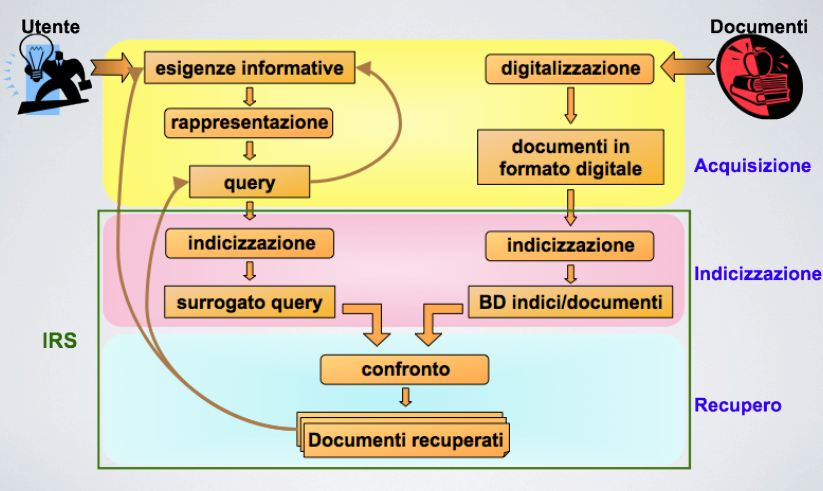
\includegraphics[width=.8\textwidth]{images/es-3-fig-1.png}
\end{figure}

Da una parte della ``U'' c'è il ramo relativo all'esigenza informativa dell'utente, la quale viene rappresentata da una query. Dall'altra parte c'è la collezione dei documenti, che contiene tutti i dati che devono essere indicizzati dal sistema in modo che possa fornire delle risposte all'utente.

Ad entrambi i rami viene poi applicato lo stesso processo di indicizzazione. Viene così ottenuta un'indice dei documenti che rappresenta in modo più semplice le informazioni contenute nei vari documenti. La stessa trasformazione subita dai documenti viene applicata in parallelo anche alla query effettuata dall'utente. 

In questo modo quando i due rami della ``U'' si congiungono nel modello di reperimento, questi possono essere facilmente confrontati tra loro. Ad esempio sia la query che i documenti della collezione possono essere rappresentati da un vettore binario che specifica se determinati termini compaiono all'interno della query/documento.

Una volta confrontata la query il sistema di reperimento produce come risultato o il documento più simile alla query, oppure una lista di documenti ordinata per similarità.

\subsection{Domanda 2}

Si effettui l'indicizzazione automatica dei documenti...

\subsection{Domanda 3}

Nel BIM la probabilità che un documento sia rilevante $P(\rel |D)$ è proporzionale al logaritmo del rapporto delle probabilità $P(\rel | D)$ e $P(\notrel | D)$. In cui $D$ è un vettore di variabili binarie.

A partire dal rapporto ottenere la formula del relevance weight:

$$
RW_i = \log \bigg( \frac{N_{t_iR} + 0.5}{N_R - N_{t_iR} +0.5} \frac{N_{NR} - N_{t_iNR} + 0.5}{N_{t_iNR} +0.5} \bigg)
$$

Utilizzando $p_i = \frac{N_{t_iR} +0.5}{N_R + 1}$.

\noindent Supponendo poi di avere la matrice 

\begin{table}[htbp]
	\centering
	\begin{tabular}{c|c|c|}
		\cline{2-3}
		& $t_1$ & $t_2$ \\ \hline
		\multicolumn{1}{|c|}{$d_1$} & 1  & 0  \\ \hline
		\multicolumn{1}{|c|}{$d_2$} & 0  & 5  \\ \hline
		\multicolumn{1}{|c|}{$d_3$} & 4  & 0  \\ \hline
		\multicolumn{1}{|c|}{$d_4$} & 0  & 3  \\ \hline
	\end{tabular}
\end{table}

\noindent calcolare i pesi per i due termini in assenza di informazioni sulla rilevanza dei documenti e senza usare la calcolatrice.

\subsubsection{Soluzione}

\begin{align}
P(\rel |D) &\propto \log \bigg( \frac{P(\rel | D)}{P(\notrel | D)} \bigg) \\
&= \log \bigg(  \frac{P(D | \rel)P(\rel)}{P(D)}  \frac{P(D)}{P(D | \notrel)P(\notrel)} \bigg) \quad \text{per Bayes}\\
&= \log \bigg(  \frac{P(D | \rel)}{P(D | \notrel)}  \underbrace{\frac{P(\rel)}{P(\notrel)}}_{\text{costante per tutta la collezione collezione}}\bigg)\\
&= \log \bigg(  \frac{P(D | \rel)}{P(D | \notrel)} \bigg)\\
&= \log \bigg(  \frac{\prod\limits_{i=1}^{|V|} P(t_i | \rel)}{\prod\limits_{i=1}^{|V|} P(t_i | \notrel)} \bigg) \quad \text{Naive bayes assumption} \\
&= \log \bigg(  \frac{\prod\limits_{i=1}^{|V|} p_i^{t_i}(1-p_i)^{1-t_i}}{\prod\limits_{i=1}^{|V|}q_i^{t_i}(1-q_i)^{1-q_i}} \bigg) \quad \text{variabili aleatori bernoulliane}\\
&= \log \bigg( \prod\limits_{i=1}^{|V|} \frac{ p_i^{t_i}(1-p_i)^{1-t_i}}{q_i^{t_i}(1-q_i)^{1-t_i}} \bigg)  \\
&= \sum\limits_{i=1}^{|V|} \log \bigg(  \frac{ p_i^{t_i}(1-p_i)^{1-t_i}}{q_i^{t_i}(1-q_i)^{1-t_i}} \bigg)\\
&= \sum\limits_{i=1}^{|V|} \log \bigg(  \frac{ \frac{p_i^{t_i}}{(1-p_i)^{t_i}}(1-p_i)  }{ \frac{q_i^{t_i}}{(1-q_i)^{t_i}}(1-q_i)  } \bigg)\\
&= \sum\limits_{i=1}^{|V|} \log \bigg(  \frac{ \bigg(\frac{p_i}{1-p_i} \bigg)^{t_i}  (1-p_i) }{ \bigg(\frac{q_i}{1-q_i}\bigg)^{t_i} (1-q_i)  } \bigg)\\
&= \sum\limits_{i=1}^{|V|} \log \bigg(   \bigg(\frac{p_i(1-q_i)}{(1-p_i)q_i} \bigg)^{t_i}  \underbrace{\frac{(1-p_i)}{(1-q_i) }}_{\text{costante per tutta la collezione}} \bigg)\\
&\propto \sum\limits_{i=1}^{|V|} t_i \log \bigg( \frac{p_i(1-q_i)}{(1-p_i)q_i} \bigg)
\end{align}

Per ottenere $RW_i$ è sufficiente espandere $p_i$ e $q_i$.

Per il secondo punto, non avendo a disposizione informazioni sui documenti rilevanti si ha che:

\begin{itemize}
\item $RW_1 = \log \bigg( \cfrac{0 + 0.5}{0 - 0 +0.5} \cfrac{4 - 2 + 0.5}{2 +0.5} \bigg) = \log\bigg(\cfrac{2.5}{2.5}\bigg) = \log(1) = 0$
\item $RW_2 = \log \bigg( \cfrac{0 + 0.5}{0 - 0 +0.5} \cfrac{4 - 2 + 0.5}{2 +0.5} \bigg) = \log\bigg(\cfrac{2.5}{2.5}\bigg) = \log(1) = 0$
\end{itemize}

\subsection{Domanda 4}

Dato un pool e una run, determinare:

\begin{enumerate}
	\item Il valore di precisione e richiamo con cut-off a 10, considerando come rilevanti tutti i documenti con grado superiore a \texttt{NR}.
	\item Il DCG della run con cut-off a 5, 10, 20 calcolato con base 10 e schema di pesatura \texttt{NR = 0, PR=5, FR=10, HR=15}
	\item Il DCG della run ideale a cut-off 15 e base 10.
\end{enumerate}

\subsubsection{Soluzione}

\begin{enumerate}
	\item $prec@10 = \cfrac{1 + 1 + 1 + 0 + 0 + 1 + 0 + 0 + 1 + 1}{10} = \cfrac{6}{10}$ e $recall@k = \cfrac{6}{12}$
	
	\item
	$$
	DCG@j = \sum\limits_{k = 1}^{j} dg_{r_t}^b[k]
	$$
	
	$$
	dg_{r_t}^b[k] = \begin{cases}
	r_t[k] & k < b \\
	\cfrac{r_t[k]}{\log_b k}
	\end{cases}
	$$
	\begin{itemize}
		\item $DCG@5 = 15 + 15 + 5 + 0 + 0 = 35$
		\item $DCG@10 = 15 + 15 + 5 + 0 + 0 + 10 + 0+ 0 + 15 + 10 = 70$
		\item $DCG@20 = DGC@10 + \cfrac{10}{\log_{10}11} + \cfrac{5}{\log_{10}12} + \ldots $
	\end{itemize}

	\item $IDCG@15 = 15 \times 4 + 10 \times 3 + 5 \times 3 + \cfrac{5}{\log_{10}11} + \cfrac{5}{\log_{10}12} + \cfrac{5}{\log_{10}13} +\cfrac{0}{\log_{10}14} +\cfrac{0}{\log_{10}15} $
\end{enumerate}

\subsection{Domanda 5}

Si presentino quali sono le differenze architetturali più significative fra un sistema di biblioteca digitale e un sistema di reperimento dell'informazione

\subsubsection{Soluzione}

Un sistema per una biblioteca digitale può essere implementato sia con un DBMS che come sistema IR.
Nel caso di un implementazione con un DBMS le interrogazioni che possono fare gli utenti sono più strutturate, ad esempio "tutti i libri scritti da" o "tutti i libri che hanno la categoria X" e i risultati forniti corrispondo ad un match deterministico della query dell'utente.

Lo stesso sistema può essere implementato anche come un IRS, in questo caso la query può anche essere più complessa, in formato narrativo e più ampia, ad esempio può essere la descrizione testuale dell'argomento trattato del libro.
Sarà poi l'IRS sottostante che si occuperà di indicizzare la query allo stesso modo dei documenti della collezione per calcolare la similarità con i documenti.

Da notare che con la versione DBMS questo tipo di interrogazione non può essere fatto, perché tipicamente nel database non viene memorizzato tutto il testo dei libri, mentre in un IRS viene utilizzato l'indice trasposto, che contiene maggiori informazioni riguardo il contenuto dei libri.

Un IRS inoltre può supportare lo stesso tipo di query di un DBMS, andando o a integrarlo, oppure ad estendere l'indice trasposto, aggiungendo dei termini extra, che non compaiono dei documenti, e che contengono l'informazione relativa agli autori e/o alla categoria del libro. Ovvero si può aggiungere all'indice un termine ``Mario Rossi'' e aggiungere alla posting-list del termini i pointer e tutti i documenti scritti da Mario Rossi.














	% !TEX encoding = UTF-8
% !TEX program = pdflatex
% !TEX root = InformationRetrieval.tex
% !TEX spellcheck = it-IT

\section{Esame 2015-06-18}

\subsection{Domanda 4}

L'approccio o il paradigma Cranfield è spesso citato come uno standard per la valutazione dei sistemi di IR: si dica che cos'è e come è stato originato.

Si dica che cos'è una collezione sperimentale di IR, quando deve essere costruita, da che elementi è composta e quali solo le metriche di base quella quale si basa.

\subsubsection{Soluzione}

Il paradigma Cranfield è un modus operandi per la valutazione dei sistemi di IR. Consiste nella modellazione di un task di ricerca di un utente, definendo a priori la collezione di documenti sulla quale si andrà a fare reperimento, le domande che verranno poste al sistema e quali sono le risposte corrette.
Così facendo è possibile replicare gli esperimenti in un secondo momento con un sistema diverso ottenendo dei risultati comparabili oppure riutilizzare le stesse collezioni per progettare nuovi esperimenti.

Questo sistema è nato per testare 4 metodi di indicizzazione per la biblioteca di Cranfield ad opera di Clevedron, il quale ha prima creato la collezione di documenti da indicizzare e definito (rivolgendosi agli autori dei documenti) le domande e le relative rispose corrette. Il primo esperimento ha richiesto 2 anni non ha fatto emergere nessun differenza tra i vari sistemi di indicizzazione a causa degli errori fatti dagli indicizzatori (era fatto tutto a mano). Tuttavia la documentazione degli esperimenti ha dato origine alla pratica della failure analisys. 

Qualche anno dopo è stato fatto un nuovo esperimento analogo, che ha tenuto conto degli errori commessi nell'impostazione del primo che ha portato alla luce delle differenze interessanti tra i vari sistemi di indicizzazione testati.

Una collezione sperimentale di IR è un'insieme di documenti per i quali sono stati definiti dei topic e dei giudizi di rilevanza (o ground truth).

$$
C = (D, T, GT)
$$

dove 

\begin{itemize}
	\item $D$ è l'insieme dei documenti della collezione
	\item $T$ è l'insieme dei topic, ovvero degli argomenti che sono trattati dai documenti della collezione.
	\item $GT$ è una funzione che associa ad un documento un giudizio di rilevanza. Sia $REL$ un insieme completamente ordinato di giudizi di rilevanza, $d \in D$ un documento e $t \in T$ un topic. $GT$ è definita come:
	\begin{align*}
		GT:  D\times T &\to REL \\
		    (d, t) &\to rel
	\end{align*}
\end{itemize}

Secondo il paradigma Cranfield la collezione di test deve essere definita prima di definire gli esperimenti, così facendo la stessa collezione può essere riutilizzata più volte, portando ad un notevole risparmio di tempo, dato che la costruzione di una collezione è molto onerosa.

Le metriche inizialmente utilizzate da Clevedron sono la precision e la recall, ma con il tempo ne sono state proposte di migliori, che prendono in considerazione anche l'andamento medio su più topic e i casi in cui i giudizi di rilevanza abbiamo più di due possibili valori.


	%\appendix
	
	%%\renewcommand{\glossaryname}{Glossario}

%\newglossaryentry{Cordova}
%{
%	name=\glslink{Cordova}{Cordova},
%	text=Cordova,
%	sort=Cordova,
%	description={Apache Cordova è un framework open source per la realizzazione di applicazioni ibride che offre delle API che permettono di accedere via JavaScript ad alcune funzionalità native del dispositivo, come l'accelerometro o la fotocamera}
%}
\subsection*{A}

\underline{\textbf{ARPA}}: %TODO

\underline{\textbf{ARPANET}}: %TODO

\underline{\textbf{Assembler}}: %TODO

\subsection*{B}

\underline{\textbf{Beowulf}}: %TODO

\subsection*{C}

\subsection*{D}

\underline{\textbf{Debian}}: %TODO

\underline{\textbf{DFSG}}: %TODO

\subsection*{E}

\subsection*{F}

\underline{\textbf{Free Software Foundation}}: %TODO

\underline{\textbf{Freeware}}: %TODO

\underline{\textbf{fsf}}: %TODO

\subsection*{G}

\underline{\textbf{GNU}}: %TODO

\underline{\textbf{GPL}}: %TODO

\subsection*{H}

\subsection*{I}

\subsection*{J}

\subsection*{K}

\underline{\textbf{Kernel}}: %TODO

\subsection*{L}

\underline{\textbf{Linux}}: %TODO

\subsection*{M}

\underline{\textbf{Mimix}}: %TODO

\underline{\textbf{MUTIX}}: %TODO

\subsection*{N}

\underline{\textbf{Netscape}}: %TODO

\underline{\textbf{nslu2}}: %TODO

\subsection*{O}

\underline{\textbf{OSI}}: %TODO

\subsection*{P}

\underline{\textbf{PDP}}: %TODO

\subsection*{Q}

\subsection*{R}

\underline{\textbf{RedHat Enterprise Linux}}: %TODO

\underline{\textbf{Routes}}: %TODO



\subsection*{S}

\underline{\textbf{StarOffice}}: %TODO

\underline{\textbf{Sun}}: 

\underline{\textbf{S\&P}}: %TODO

\underline{\textbf{Shareware}}: %TODO

\underline{\textbf{Symbolics}}: %TODO	

\subsection*{T}

\underline{\textbf{TECO}}: %TODO

\subsection*{U}

\underline{\textbf{Unix}}: %TODO

\subsection*{V}

\subsection*{W}

\subsection*{X}

\subsection*{Y}

\subsection*{Z}


	




	
	
\end{document}